% Options for packages loaded elsewhere
% Options for packages loaded elsewhere
\PassOptionsToPackage{unicode}{hyperref}
\PassOptionsToPackage{hyphens}{url}
%
\documentclass[
  spanish,
  11pt,
  a4paper,
]{scrbook}
\usepackage{xcolor}
\usepackage[left=3cm,right=3cm,top=3cm,bottom=4cm]{geometry}
\usepackage{amsmath,amssymb}
\setcounter{secnumdepth}{-\maxdimen} % remove section numbering
\usepackage{iftex}
\ifPDFTeX
  \usepackage[T1]{fontenc}
  \usepackage[utf8]{inputenc}
  \usepackage{textcomp} % provide euro and other symbols
\else % if luatex or xetex
  \usepackage{unicode-math} % this also loads fontspec
  \defaultfontfeatures{Scale=MatchLowercase}
  \defaultfontfeatures[\rmfamily]{Ligatures=TeX,Scale=1}
\fi
\usepackage{lmodern}
\ifPDFTeX\else
  % xetex/luatex font selection
  \setmainfont[]{Cormorant Garamond}
\fi
% Use upquote if available, for straight quotes in verbatim environments
\IfFileExists{upquote.sty}{\usepackage{upquote}}{}
\IfFileExists{microtype.sty}{% use microtype if available
  \usepackage[]{microtype}
  \UseMicrotypeSet[protrusion]{basicmath} % disable protrusion for tt fonts
}{}
\makeatletter
\@ifundefined{KOMAClassName}{% if non-KOMA class
  \IfFileExists{parskip.sty}{%
    \usepackage{parskip}
  }{% else
    \setlength{\parindent}{0pt}
    \setlength{\parskip}{6pt plus 2pt minus 1pt}}
}{% if KOMA class
  \KOMAoptions{parskip=half}}
\makeatother
% Make \paragraph and \subparagraph free-standing
\makeatletter
\ifx\paragraph\undefined\else
  \let\oldparagraph\paragraph
  \renewcommand{\paragraph}{
    \@ifstar
      \xxxParagraphStar
      \xxxParagraphNoStar
  }
  \newcommand{\xxxParagraphStar}[1]{\oldparagraph*{#1}\mbox{}}
  \newcommand{\xxxParagraphNoStar}[1]{\oldparagraph{#1}\mbox{}}
\fi
\ifx\subparagraph\undefined\else
  \let\oldsubparagraph\subparagraph
  \renewcommand{\subparagraph}{
    \@ifstar
      \xxxSubParagraphStar
      \xxxSubParagraphNoStar
  }
  \newcommand{\xxxSubParagraphStar}[1]{\oldsubparagraph*{#1}\mbox{}}
  \newcommand{\xxxSubParagraphNoStar}[1]{\oldsubparagraph{#1}\mbox{}}
\fi
\makeatother


\usepackage{longtable,booktabs,array}
\newcounter{none} % for unnumbered tables
\usepackage{calc} % for calculating minipage widths
% Correct order of tables after \paragraph or \subparagraph
\usepackage{etoolbox}
\makeatletter
\patchcmd\longtable{\par}{\if@noskipsec\mbox{}\fi\par}{}{}
\makeatother
% Allow footnotes in longtable head/foot
\IfFileExists{footnotehyper.sty}{\usepackage{footnotehyper}}{\usepackage{footnote}}
\makesavenoteenv{longtable}
\usepackage{graphicx}
\makeatletter
\newsavebox\pandoc@box
\newcommand*\pandocbounded[1]{% scales image to fit in text height/width
  \sbox\pandoc@box{#1}%
  \Gscale@div\@tempa{\textheight}{\dimexpr\ht\pandoc@box+\dp\pandoc@box\relax}%
  \Gscale@div\@tempb{\linewidth}{\wd\pandoc@box}%
  \ifdim\@tempb\p@<\@tempa\p@\let\@tempa\@tempb\fi% select the smaller of both
  \ifdim\@tempa\p@<\p@\scalebox{\@tempa}{\usebox\pandoc@box}%
  \else\usebox{\pandoc@box}%
  \fi%
}
% Set default figure placement to htbp
\def\fps@figure{htbp}
\makeatother

\ifLuaTeX
  \usepackage{luacolor}
  \usepackage[soul]{lua-ul}
\else
  \usepackage{soul}
\fi


\ifLuaTeX
\usepackage[bidi=basic,shorthands=off]{babel}
\else
\usepackage[bidi=default,shorthands=off]{babel}
\fi
\ifPDFTeX
\else
\babelfont{rm}[]{Cormorant Garamond}
\fi
\ifLuaTeX
  \usepackage{selnolig} % disable illegal ligatures
\fi


\setlength{\emergencystretch}{3em} % prevent overfull lines

\providecommand{\tightlist}{%
  \setlength{\itemsep}{0pt}\setlength{\parskip}{0pt}}



 
\usepackage[refsection=chapter,style=apa,isbn=false]{biblatex}
\addbibresource{Libro.bib}


% ==============================================================================
% CONFIGURACIÓN GLOBAL DEL LIBRO (Unificación Definitiva - Libro 1)
% ==============================================================================

% --- 1. Fuentes y Tipografía Replicables (Solución Física Mac) ---
\usepackage{fontspec}
\setmainfont{Cormorant Garamond}[
    UprightFont = *-Medium
]
\setsansfont{Montserrat-Regular.otf}[
    BoldFont = Montserrat-SemiBold.otf
]

% --- 2. Ajustes de Párrafo y Espaciado Vertical (Estilo Refinado) ---
\usepackage{widows-and-orphans}
\widowpenalty=10000
\clubpenalty=10000
\setlength{\parindent}{1.2em} % Sangría de primera línea ganadora
\setlength{\parskip}{0pt}     % Sin espacios vacíos entre párrafos ordinarios

\usepackage{setspace}
\setstretch{1.3}              % Interlineado sofisticado y compacto

% --- 3. Jerarquía y Alineación de Títulos (KOMA-Script) ---
\addtokomafont{disposition}{\sffamily\fontspec{Montserrat-SemiBold.otf}}
\addtokomafont{chapter}{\huge\raggedright}
\addtokomafont{section}{\Large\raggedright}
\addtokomafont{subsection}{\normalsize}

% --- 4. Encabezados y Pies de Página (Mantenido de tu estructura) ---
\usepackage{scrlayer-scrpage}
\automark{chapter}

% --- 5. Gestión de Gráficos e Imágenes ---
\usepackage{graphicx}
\graphicspath{{../assets/imagenes/}{../../institucionales/assets/logos/}}

% --- 6. Ajustes Finos de Disposición de Capítulos ---
\addtokomafont{disposition}{\linespread{1.2}\selectfont}
\RedeclareSectionCommand[
    beforeskip=-0.0cm,
    afterskip=1.5cm
]{chapter}

% ==============================================================================
% CONFIGURACIÓN DE IDIOMA Y CONECTORES PARA BIBLATEX (ESTILO APA)
% ==============================================================================

% 1. Definir las cadenas de traducción oficiales al español
\DefineBibliographyStrings{spanish}{%
  and = {y},
  andothers = {et~al.},
  volume = {vol.},
  volumes = {vols.},
  pages = {pp.},
  page = {p.}
}

% 2. Forzar al estilo APA a usar la "y" en lugar del ampersand (&) en los textos e índices
\DeclareDelimFormat*{finalnamedelim}{\addspace\bibstring{and}\addspace}
\DeclareDelimFormat*{finalnamedelim:apaenum}{\addspace\bibstring{and}\addspace}
% ==============================================================================
% ENSTORNOS Y COMANDOS PERSONALIZADOS (Especial para Etnografía y Entrevistas)
% ==============================================================================

% --- 1. Paquetes requeridos para control de listas y color ---
\usepackage{enumitem}
\usepackage{xcolor}

% --- 2. Entorno para transcripciones de entrevistas estructuradas ---
% Corrige espaciados para que los fragmentos no queden flotando o muy separados
\newenvironment{transcripcion}{
    \begin{list}{}{
        \setlength{\leftmargin}{1.5em}  % Un toque más de entrada para notar el bloque
        \setlength{\rightmargin}{0em}
        \setlength{\itemsep}{0.2em}     % Ajuste fino de separación entre réplicas
        \setlength{\parsep}{0.0em}
        \setlength{\listparindent}{0pt}
    }
}{
    \end{list}
}

% --- 3. Comandos auxiliares para dinamismo de diálogos etnográficos ---
% \personaje{Nombre}: Renderiza el actor social en negrita con un espacio elegante
\newcommand{\personaje}[1]{\textbf{#1}\quad}

% \escena{Texto}: Ideal para descripciones de diario de campo o gestos en cursiva y chica
\newcommand{\escena}[1]{\textit{\small #1}\par\vspace{0.4em}}
\makeatletter
\@ifpackageloaded{bookmark}{}{\usepackage{bookmark}}
\makeatother
\makeatletter
\@ifpackageloaded{caption}{}{\usepackage{caption}}
\AtBeginDocument{%
\ifdefined\contentsname
  \renewcommand*\contentsname{Tabla de contenidos}
\else
  \newcommand\contentsname{Tabla de contenidos}
\fi
\ifdefined\listfigurename
  \renewcommand*\listfigurename{Listado de Figuras}
\else
  \newcommand\listfigurename{Listado de Figuras}
\fi
\ifdefined\listtablename
  \renewcommand*\listtablename{Listado de Tablas}
\else
  \newcommand\listtablename{Listado de Tablas}
\fi
\ifdefined\figurename
  \renewcommand*\figurename{Figura}
\else
  \newcommand\figurename{Figura}
\fi
\ifdefined\tablename
  \renewcommand*\tablename{Tabla}
\else
  \newcommand\tablename{Tabla}
\fi
}
\@ifpackageloaded{float}{}{\usepackage{float}}
\floatstyle{ruled}
\@ifundefined{c@chapter}{\newfloat{codelisting}{h}{lop}}{\newfloat{codelisting}{h}{lop}[chapter]}
\floatname{codelisting}{Listado}
\newcommand*\listoflistings{\listof{codelisting}{Listado de Listados}}
\makeatother
\makeatletter
\makeatother
\makeatletter
\@ifpackageloaded{caption}{}{\usepackage{caption}}
\@ifpackageloaded{subcaption}{}{\usepackage{subcaption}}
\makeatother
\usepackage{bookmark}
\IfFileExists{xurl.sty}{\usepackage{xurl}}{} % add URL line breaks if available
\urlstyle{same}
% fallback for those not using the hyperref driver hyperxmp:
\makeatletter
\@ifundefined{xmpquote}{\newcommand{\xmpquote}[1]{#1}}{}
\makeatother
\hypersetup{
  pdftitle={Políticas Públicas y Etnografía},
  pdflang={es},
  hidelinks,
  pdfcreator={LaTeX via pandoc}}


\title{Políticas Públicas y Etnografía}
\usepackage{etoolbox}
\makeatletter
\providecommand{\subtitle}[1]{% add subtitle to \maketitle
  \apptocmd{\@title}{\par {\large #1 \par}}{}{}
}
\makeatother
\subtitle{Observando al Estado y como el Estado}
\author{}
\date{}
\begin{document}
\frontmatter
\maketitle

% ============================================
% DEFINICIÓN DE FUENTE PARA LA PORTADA
% ============================================
\newfontfamily\montserrat[
  Path=assets/fuentes/Montserrat/static/,
  Extension=.ttf,
  BoldFont=Montserrat-SemiBold,
  ItalicFont=Montserrat-Italic  % Si no existe, fontspec usará slant sintético
]{Montserrat-Regular}

%=============================================================================
% PÁGINA 2: PORTADA FULL-PAGE
%=============================================================================
{

\thispagestyle{empty}

\hoffset=-1in
\voffset=-1in
\oddsidemargin=0pt
\evensidemargin=0pt
\topmargin=0pt
\headheight=0pt
\headsep=0pt

\noindent
% El comando \lower agarra la caja de ancho cero y la desplaza hacia abajo de forma obligatoria.
% Empezamos con 1.8cm. Si notas que le falta bajar un poco, súbelo a 2.5cm.
\lower 1.8cm \hbox to \paperwidth{%
    \hss
    \includegraphics[width=\paperwidth,height=1.0\paperheight,keepaspectratio=false]{assets/imagenes/libro2portada2026.pdf}%
    \hss
}

\clearpage

}
% ============================================
% PÁGINA 2: EN BLANCO (verso de portada)
% ============================================
\clearpage
\thispagestyle{empty}
\null
\clearpage

% ============================================
% PÁGINA 3: PORTADILLA (MEDIA PORTADA)
% ============================================
\clearpage
  \thispagestyle{empty}
  \begingroup
    \raggedright
    \vspace*{1cm}
    \sffamily\small
    \montserrat\huge Políticas Públicas y Etnografía \\
    \vspace{0.3cm}
    {\Large Observando al Estado y como el Estado} \\
    \vspace{0.7cm}
    {\Large Abraham Zaíd Díaz Delgado} \\
    \vspace{0.3cm}
    \Large\rmfamily\textit{Coordinador}
    \vfill
  % Centrado exacto de la imagen
  \begin{center}
    
\includegraphics[width=0.4\textwidth]{../../assets/logos/logoUAML.png}
  \end{center}
  
  \vspace{1cm} % Espacio de respiro antes del corte de página
  \endgroup
\clearpage

% ==============================================================================
% PÁGINA 4: DIRECTORIO INSTITUCIONAL CENTRADO
% ==============================================================================
\clearpage
  \begingroup
    \thispagestyle{empty}
      \begin{center}
        \sffamily\small
        {\montserrat\Large\textbf{UNIVERSIDAD AUTÓNOMA METROPOLITANA}} \\
        {\montserrat\large\textbf{RECTORÍA GENERAL}} \\
        \vspace{0.2cm}
        \textit{Dr. Raúl Gustavo Pacheco López} \\
        Rector \\
        \vspace{0.1cm}
        {\itshape Dra. Esthela Irene Sotelo Núñez} \\
        Secretaria General\\
        
        \vspace{0.1cm}
        \rule{0.6\textwidth}{0.4pt}
        \vspace{0.1cm}
        
        {\montserrat\large\textbf{UNIDAD LERMA}} \\
        \vspace{0.2cm}
        \textit{Dra. Alma Patricia de León Calderón} \\
        Rectora \\
        \vspace{0.1cm}
        {\itshape Dra. Karla Pelz Serrano} \\
        Secretaria \\
        \vspace{0.1cm}
        {\montserrat\large\textbf{División de Ciencias Sociales y Humanidades}} \\
        \vspace{0.1cm}
        \textit{Dr. Raúl Hernández Mar} \\
        Director \\
        \vspace{0.1cm}
        \textit{Dra. Ana Carolina Robles Salvador} \\
        Secretaria Académica \\
  
        %\vspace{0.1cm}
        \rule{0.6\textwidth}{0.4pt}
        %\vspace{0.1cm}
  
        {\montserrat\large\textbf{Consejo Editorial - Publicaciones Periódicas}} \\
        %{\montserrat\normalfont{Publicaciones Periódicas}} \\
        \vspace{0.2cm}
        \textit{Abigail Martínez Mendoza} \\
        Coordinadora General \\
        \vspace{0.1cm}
        \textit{Omar Valencia Domínguez} \\
        \textit{Ryszard Edward Rozga Luter} \\
        Departamento de Procesos Sociales \\
        \vspace{0.1cm}
        \textit{José Omar Pérez Baños} \\
        Departamento de Estudios Culturales \\
        
        %\vspace{0.1cm}
        \rule{0.6\textwidth}{0.4pt}
        %\vspace{0.1cm}
        
        {\montserrat\large\textbf{Edición Técnica, Corrección de Estilo y Diseño}} \\
        \vspace{0.2cm}
        \textit{José Omar Pérez Baños} \\
        Director del Equipo Editorial \\
        \vspace{0.1cm}
        \textit{Jonathan Armando Chávez Solís} \\
        Editor Literario\\
        \textit{Yunuen Rosas Ortiz} \\
        Ilustradore \\
      \end{center}
  \endgroup
\clearpage

% ==============================================================================
% PÁGINA 5: PÁGINA LEGAL ESTÁNDAR (DCSH - UAM LERMA)
% ==============================================================================
\clearpage
\thispagestyle{empty}
\begin{center}
    % --- Ficha de Catalogación Superior ---
    \framebox[\textwidth]{\vbox{
        \vspace{0.3cm}
        \hbox to \textwidth{\hfill\montserrat\scriptsize\textbf DATOS DE CATALOGACIÓN\hfill}
        \vspace{0.2cm}
        \noindent\hspace{0.5cm}
        \parbox{0.9\textwidth}{
            \rmfamily\scriptsize
            \texttt{Díaz Delgado, Abraham Zaíd (coordinador)} \\
            Políticas Públicas y Etnografía : Observando al Estado y como el Estado / Abraham Zaíd Díaz Delgado, coordinador. -- México : Universidad Autónoma Metropolitana : Unidad Lerma : División de Ciencias Sociales y Humanidades, 2026. \\
            \quad p. : il. ; 14 x 21 cm. \\
            \quad ISBN: 978-xxx-xxx-xxx-x \\
            \quad 1. Políticas públicas -- Aspectos sociales. 2. Antropología política -- Etnografía política. 3. Etnografía del Estado -- Etnografía de las instituciones. 4. Etnografía -- Metodología -- México. 5. Reflexividad. I. Universidad Autónoma Metropolitana. Unidad Lerma. División de Ciencias Sociales y Humanidades.
        }
        \vspace{0.3cm}
    }}
\end{center}

\vspace*{\fill} % Empuja los datos legales al fondo de la página

% --- Créditos y Derechos de Autor ---

\begingroup
\begin{singlespace}
\fontspec{Montserrat-Regular.otf}\scriptsize
\noindent
Primera edición: 2026\\
Políticas Públicas y Etnografía : Observando al Estado y como el Estado\\
Abraham Zaíd Díaz Delgado, coordinador\\[0.5em]
Diseño de portada: Yunuen Rosas Ortíz\\[0.5em]
D.R. © 2026, Universidad Autónoma Metropolitana\\
Prolongación Canal de Miramontes 3855, Ex Hacienda San Juan de Dios,\\
Alcaldía de Tlalpan, C.P. 14387, Ciudad de México.\\[0.5em]
{\fontspec{Montserrat-SemiBold.otf}\scriptsize Universidad Autónoma Metropolitana, Unidad Lerma}\\
División de Ciencias Sociales y Humanidades\\
Consejo Editorial de la División de Ciencias Sociales y Humanidades\\
Avenida de las Garzas núm. 10, Col. El Panteón,\\
C.P. 52005, Lerma de Villada, Estado de México.\\
Contacto: \href{mailto:cedcsh@correo.ler.uam.mx}{cedcsh@correo.ler.uam.mx}\\[0.8em]
ISBN: 978-xxx-xxx-xxx-x\\[0.8em]
Esta publicación no puede ser reproducida, ni en todo ni en parte, ni registrada o transmitida por un sistema de recuperación de información, en ninguna forma ni por ningún medio, sea mecánico, fotoquímico, electrónico, magnético, electroóptico, por fotocopia o cualquier otro, sin el permiso previo y por escrito de los editores.\\[0.5em]
La presente publicación pasó por un proceso de dos dictámenes (doble ciego) de pares académicos avalados por el Consejo Editorial de la División de Ciencias Sociales y Humanidades de la UAM-Lerma, que garantizan su calidad y pertinencia académica y científica.\\[0.5em]
Publicación digital hecha en México / Digital publication made in Mexico
\end{singlespace}
\endgroup
\clearpage

% ============================================
% PÁGINA EN BLANCO
% ============================================
\clearpage
\thispagestyle{empty}
\null
\clearpage

\renewcommand*\contentsname{Índice}
{
\setcounter{tocdepth}{1}
\tableofcontents
}

\mainmatter
\bookmarksetup{startatroot}

\chapter*{Observando al Estado y como el
Estado.}\label{observando-al-estado-y-como-el-estado.}
\addcontentsline{toc}{chapter}{Observando al Estado y como el Estado.}

\markboth{Observando al Estado y como el Estado.}{Observando al Estado y
como el Estado.}

\vspace{-\baselineskip}

\section*{Presentación}\label{presentaciuxf3n}

\markright{Presentación}

\addtocontents{toc}{\protect\hspace{1.5em}Abraham Zaíd Díaz Delgado\par}

Las políticas públicas (PP) repercuten en nuestras vidas, pues suponen
el funcionamiento de los engranajes políticos que los Estados nacionales
ponen en marcha para dar solución a circunstancias identificadas como
problemáticas dentro del orden social vigente. No es casualidad que su
estudio se centre en comprender qué hacen los gobiernos para que la
maquinaria opere tal como lo hace, con sus fallas ineludibles y sus
puntos perfectibles. Asimismo, permiten reflexionar en profundidad sobre
las razones que dan origen al orden dispuesto de los engranajes de la
maquinaria gubernamental, cuestionándose ¿por qué las piezas se
encuentran en esa posición y no en otra?, ¿cómo debe resolverse
determinado problema?, ¿qué tuvo que suceder para que una realidad fuera
reconocida como un problema que solo el Estado puede resolver? Y, sobre
todo, ¿por qué en muchas ocasiones no logra darle solución? De este
modo, continúan surgiendo interrogantes sobre los efectos que las
potenciales soluciones tienen en realidad, dado que las políticas
públicas son, en esencia, una compleja matriz de toma de decisiones
humanas guiadas por el imperativo ideológico que reivindica la
legitimidad del Estado y de sus instituciones. Bajo este enfoque,
resulta necesario indagar, en un nivel empírico, en la experiencia de
los diversos agentes que participan en el complejo entramado de fuerzas
políticas que conforman las políticas públicas.

Cuando James C. \textcite{Scott1998} se preguntó por las razones que han
llevado a los proyectos estatales al fracaso, reconoció la existencia de
una razón de Estado, esto es, de una forma particular de interpretar y
proceder hacia su otredad más evidente: la sociedad civil. Para este
antropólogo político norteamericano, esa forma de pensamiento
corresponde a una posición específica del ejercicio del poder, desde la
cual se vuelve ineludible adoptar la visión proestatal, especialmente
desde las burocracias \autocite{Graeber2019} y con base en la
hiperespecialización técnica \autocite{Mitchell2002}.

Este libro colectivo, ``Políticas Públicas y Etnografía. Observando al
Estado y como el Estado'', representa un esfuerzo por impulsar el
pensamiento crítico de esa razón de Estado, reconociendo que esta se
expresa simultáneamente en niveles materiales y simbólicos; es decir,
tanto en ideas y discursos como en hechos cotidianos concretos
\autocite{Abrams1977}, que merecen introducirse al debate académico
interdisciplinario desde una aproximación empírica.

He de advertir a los lectores que este no es un compilado de desarrollo
riguroso de los marcos teóricos hegemónicos en el estudio de las
políticas públicas (PP). Este libro también está lejos de lo que pudiera
pensarse como antropología aplicada \autocite{Garrison1895}, disciplina
que posee una longeva tradición de coadyuvar esfuerzos fuera de la
academia para atender problemas sociales, culturales, políticos y
económicos. Más bien, aquí se busca realizar un recorrido distinto en el
cual se devuelva el producto de esos esfuerzos al debate dentro de las
ciencias sociales y humanidades, porque, comúnmente, los investigadores
conservan preocupaciones e intereses marginados del locus de enunciación
científico que pueden contribuir a construir nuevas y mejores propuestas
investigativas, redefinir procedimientos técnicos o burocráticos y,
esencialmente, a pensar de forma distinta las acciones del Estado, ya
sea cuando este constituye una otredad o cuando se está inmerso en sus
instituciones formales.

Una de las principales motivaciones para emprender esta obra es la
necesidad de reconocer las distintas formas de conocimiento que
comparten los espacios académicos y administrativos o ejecutivos
estatales, siendo las políticas públicas un punto de encuentro común.

En estas páginas se recogen una serie de reflexiones profundas derivadas
de las experiencias específicas de investigadores que participaron en
alguna fase del ciclo de las políticas públicas y que, aplicando sus
conocimientos en distintos escenarios, se han enfrentado al peso de la
razón estatal y han logrado conservar una postura crítica frente a esta.
En este sentido, las experiencias etnográficas que aquí se presentan
constituyen fuentes valiosas para dar continuidad a un aprendizaje
colectivo, siendo capaces de atenuar la atomización de los esfuerzos
investigativos y de replantear la visión común que considera los
resultados del estudio de las PP como procesos distantes, fríos,
impersonales y estériles. De esta forma se permite a quien lea cada una
de las contribuación adentrarse en los mundos de significados
autocontenidos en el universo de las políticas públicas valorando la
diversidad de voces, posiciones y experiencias en la atención de
problemáticas sociales particulares.

A partir de lo anterior cabe preguntarse cuáles son los alcances reales
de la diferencia hermenéutica entre ver y observar: ver como lo hace el
Estado de acuerdo con la crítica referida de James C. Scott (1998), y
observar como elemento central de la etnografía en su triple dimensión:
como método, herramienta y descripción (Guber, 2001). De ese modo, la
etnografía llega a ofrecer la posibilidad de unir campos prácticos y
analíticos típicamente distintos en condiciones específicas y en
múltiples niveles. Otra pregunta que vale la pena formularse es `¿quién
observa al Estado?, entendiendo que la observación no es una acción
pasiva, sino dinámica y reflexiva a la vez; por tanto, sumamente
complicada de realizar. Además, ¿desde dónde es posible observar al
Estado?

Este libro trata de ofrecer una amplia gama de respuestas ante estas
preguntas para inaugurar un debate, más que llegar a una generalización
concluyente. La propuesta que convoca a los autores de este libro es
reconocer al Estado como objeto de estudio desde la experiencia dentro y
fuera de él. Cabe advertir al lector que esto no es lo habitual y que,
precisamente en ello, radica el valor de este trabajo conjunto.

\vspace*{.5cm}

Los trabajos de investigación reunidos en este libro constituyen una
selección de material idóneo para abordar las preguntas planteadas,
además de permitir la identificación de casos de referencia y la
realización de estudios de política comparada. En cada uno de ellos
también se ofrecen las descripciones densas elaboradas por los autores
que, en la mayoría de los casos, ocuparon posiciones privilegiadas desde
las cuales lograron reconocer tanto las virtudes como las áreas de
oportunidad en el abordaje de los problemas sociales contemporáneos a
través de políticas públicas específicas.

En el primer capítulo, Abraham Zaíd Díaz Delgado revisita
etnográficamente su experiencia profesional en la dependencia operadora
de la política de telecomunicaciones en México durante los años 2024 y
2025, mostrando que, en el seno de las políticas públicas, se debaten y
definen distintas perspectivas de la idea hegemónica del Estado, así
como del discurso gubernamental de la llamada ``Cuarta Transformación''
(4T), en este caso particular. Destaca que la política de
telecomunicaciones funge como punto de encuentro entre el desarrollo
tecnológico y la consolidación de un régimen político.

En lo que toca a los retos de la PP del sector, se reconoce la necesidad
de superar la contradicción entre el discurso de justicia social de la
4T y la complejidad real que esta implica, así como el hecho de que la
política de telecomunicaciones es reflejo de dicha inconsistencia.
Además, señala que la superación de la brecha digital está atravesada
por sesgos de carácter técnico que no son necesariamente vinculantes con
la dignificación de los medios de vida de las poblaciones incomunicadas.
Otro aspecto que remarca este trabajo es que la brecha digital reproduce
brechas sociales de clase, lo que la convierte en un fenómeno
predominantemente político.

Asimismo, el texto ilustra la coyuntura política del cambio
institucional en México con la llegada al poder del partido MORENA,
proceso que ha generado contradicciones y desaciertos en la operación de
las PP. Pero, principalmente, abre un panorama novedoso sobre el
potencial explicativo de la etnografía para el ciclo de las políticas
públicas, no solo como un método de extracción de información para su
diagnóstico, implementación y evaluación, sino también como una
herramienta aplicada a los mecanismos internos y a los andares
cotidianos que involucran a funcionarios públicos, operadores de las PP
y población beneficiaria, desde una lectura crítica de la antropología y
etnografía política, del Estado, la ley y las instituciones,
introduciendo una vía analítica no exenta de originalidad para las
ciencias sociales y la función pública.

\vspace*{.75cm}

En el segundo capítulo Marco Rodríguez y Nancy Jiménez analizan el
impacto de la política social del régimen de gobierno actual en México,
autodenominado de ``la cuarta transformación'' (4T), en los trabajadores
formales e informales del sector de residuos, específicamente en
Acapulco (Guerrero), Oaxaca de Juárez (Oaxaca), Tlaxcala (Tlaxcala) y
Cuetzalan (Puebla) con aquellos que cumplen las tareas de procesamiento,
recolección, traslado y tratamiento de desechos sólidos.

El estudio emplea un enfoque mixto que abona al diálogo entre la
profundidad descriptiva con visión panorámica de los datos estadísticos
e indicadores de evaluación a fin de proponer una alineación entre
políticas públicas a diversas escalas y niveles de gobierno. La
pertinencia de esta investigación radica en tomar como punto de partida
el perfil socioeconómico de los trabajadores resultando que, debido a la
condición marginal en la que suelen vivir, son objeto de múltiples
programas de asistencia social, en un principio, porque la cobertura de
manutención que otorga su remuneración como trabajadores del sector de
residuos es insuficiente.

Aunado a ello, la aplicación a formar parte de otros programas sociales
acarrea una serie de obstáculos que deben sortear y que recrudecen la
condición de vulnerabilidad en la que están sumergidas sus familias.
Otra virtud del trabajo de los autores es reconocer la desigualdad como
una condición sine qua non para determinadas políticas sociales y la
recolección de datos en diversos contextos dentro del territorio
mexicano demuestra que fungen también como mecanismos de diferenciación
revitalizando diversas violencias, sobre todo la económica, de manera
estructural. Con todo, la corrección que promueve el capítulo insta a
alineamiento de multiescalar de la política social para dignificar la
vida de los sectores marginados y puntualmente del sector laboral de la
gestión de residuos sólidos.

\vspace*{.75cm}

El tercer capítulo autoría de Enver Vargas y David Alzate profundiza en
el análisis crítico de categorías dominantes que fundan las bases sobre
las cuales se diseña, implementa y evalúan las políticas públicas desde
la valoración de la subjetividad y reflexividad en la investigación,
dichas categorías se reflejan en la noción del Estado como ente unitario
o monolítico, la legitimidad en el actuar gubernamental y la
impersonalidad con que la burocracia asume a las personas,
objetivándolas y despojándolas en la práctica de su calidad de sujetos
de derecho cuando han de entrar en acción los fundamentos estatales para
su protección como lo son las políticas públicas.

Los autores ---de origen colombiano--- comparten las etnografías de dos
casos concretos en su país para ello; el primero de ellos aborda la
operación del Programa de Defensoría del Pueblo en un momento de
emergencia humanitaria frente a las violaciones de derechos humanos
perpetradas en el contexto de los años del conflicto armado por las
guerrillas en aquel país y el segundo expone una red criminal en el
Departamento Administrativo de Seguridad luego de encontrarse culpables
a diversos funcionarios públicos que colaboraron en el despliegue
criminal en ese mismo contexto. Es importante reconocer que ambos casos
de estudio oscilan entre la ``técnica y la política'' a decir que los
autores, dejando de manifiesto una posición parcial y pragmática
necesaria para poder desarrollar una exploración etnográfica de mayor
alcance y multivocal, esto es algo que constantemente ha de hacerse en
casos de corrupción y violencia como los aquí atendidos.

Por si fuera poco, hace presencia otro tipo de abordaje etnográfico
conocido como ``etnografía documental'' que somete a cuestionamiento las
estructuras que consolidan los archivos y documentos que soportan los
relatos comúnmente hegemónicos de un momento histórico, por lo común, en
entornos de riesgo y conflicto esta clase de etnografía es de gran
utilidad; siendo este capítulo un claro ejemplo. En suma, Vargas y
Alzate demuestran el borramiento y superación de las nociones de
típicamente evocan la idea de Estado, sus procesos y políticas
securitarias que, específicamente en Colombia se ven excedidos en la
atención del trauma emanado del conflicto armado y porque ese daño se
produjo, en parte, por el entrelazamiento entre estatalidad y
criminalidad.

\vspace*{.75cm}

El capítulo cuatro coescrito por Omar Becerra, Tzitzi Becerra y
Francisco Ayala se ocupa de analizar el estado vigente de las políticas
públicas orientadas a la preservación y promoción de los patrimonios
culturales del estado de Michoacán, México, alertando sobre la
parcialidad de éstas y la necesidad de estrechar la vinculación con las
comunidades por el desconocimiento de las necesidades culturales reales
de la población incluyendo factores de orden económico, social y
ambiental a las políticas públicas locales en torno al patrimonio
cultural michoacano, afinando así el proceso de éstas y evitando su
operación de manera aislada como mecanismo de gobierno.

Además, se expone desde una perspectiva histórica el proceso
institucional y legal que rige hasta el día de hoy el entorno político
del patrimonio material e inmaterial con el que cuenta Michoacán, lejos
de centrarse en un programa o bien cultural específico, los autores
demuestran elementos contextuales sobre los cuales la etnografía se
presenta como una alternativa viable para la mejora de las políticas
públicas culturales, de las instituciones que las construyen y ejecutan,
así como de la construcción discursiva de la riqueza cultural y
patrimonial local.

Finalmente, este capítulo colectivo sugiere que el aumento del
financiamiento estatal para fortalecer las cadenas de valor existentes
en materia cultural y, sobre todo, destaca la necesidad de involucrar a
las comunidades objetivo en el establecimiento de una agenda cultural
para un correcto diagnóstico e implementación de las políticas públicas
culturales en Michoacán.

\vspace*{.75cm}

En el capítulo quinto Alejandro Agudo ilustra las complejidades que
alberga la construcción de conocimiento y toma de decisiones en las
posiciones de ``antropólogo activista'' y ``antropólogo consultor''
empleando dos ejemplos prácticos que contrastan las condiciones,
directrices y demandas de cada escenario, si bien ambos contextos son
distintos, en ellos coincide la etnografía como parte central de las
funciones desarrolladas por el antropólogo y dan pie a cuestionamientos
profundos sobre la posibilidad de conciliar entre el activismo y la
consultoría orientados a la atención de poblaciones vulnerables.

En este trabajo el autor advierte desde su experiencia acumulada que
existen algunos riesgos y condicionamientos interpretativos involucrados
en estos distintos entornos de aplicación y construcción del
conocimiento, siendo quizá el más claro, la tendencia a caer en polos
opuestos de la práctica etnográfica.

Por un lado, señala que la adopción de una postura moral denunciante
útil para evidenciar los legítimos reclamos por justicia de sectores
marginados sistemáticamente puede llevar al punto de imposibilitar la
visualización de soluciones de los problemas que les aquejan e incluso
reforzando una visión parcial del origen de dichos problemas, así como
obstaculizar el entendimiento de las formas en cómo funciona la realidad
social más amplia, lo que derivaría un diagnóstico sesgado y limitante
de la vulnerabilidad referida.

Por otra parte, aborda empíricamente la incidencia de agendas políticas
externas a las instituciones, dependencias, organismos y demás
instancias encargadas de llevar a cabo proyectos de consultoría que
tienen a como prioridad idear, articular, promover y emprender
soluciones a problemas puntuales para determinados sectores, mismas que
derivan en procedimientos y tratamientos de información que tiende a
homogenizar los resultados en informes, recomendaciones o archivos que
desdibujan la profundidad reflexiva de la etnografía y que pocas veces
se basan realmente en las reflexiones derivadas de ésta, uno de los
factores transversales a estas agendas es el tiempo, puesto que la
etnografía deviene necesariamente en una honda reflexión que lleva
tiempo procesar y expresar en los términos adecuados para su aplicación
en contextos donde potencialmente podría incidir.

Finalmente, este capítulo cumple con uno de los fines esenciales de este
libro al poner en debate las contradicciones y tensiones éticas que se
han definido típicamente unos espacios como académicos y otros como
aplicados casi exclusivamente.

\vspace*{.75cm}

Virginia Ramírez presenta en el sexto capítulo los efectos que ha tenido
el levantamiento del muro fronterizo de los Estados Unidos para marcar
la división con el territorio mexicano en una colonia marginal de
Tijuana (Baja California) generando la reconfiguración del paisaje
urbano a través del desalojo y despojo de viviendas para construir
vialidades que agilicen la movilidad en esa ciudad.

El capítulo de la antropóloga va más allá de las políticas públicas como
medio de acción de un estado nacional, ya que el contexto de la frontera
norte de México se ve influido por la actual crisis de movilidad humana
a escala global, siendo la ciudad referida en esta etnografía donde se
da el flujo de migrantes más numeroso de todo el mundo.

La investigación se inscribe en el contexto del programa federal
``Viaducto Elevado Tijuana'', un megaproyecto de infraestructura
emprendido por el Estado mexicano para dar abasto a la movilidad de la
zona y que no solo ha generado cambios en la concepción del espacio
público, sino que ha devenido en un punto de quiebre de las historias de
vida de los habitantes de la colonia Libertad. El capítulo muestra la
yuxtaposición de políticas públicas que no se encuentran alineadas dada
la preeminencia de agendas que obedecen a intereses políticos, factores
económicos y a la gestión de crisis que desplazan y criminalizan
familias además de precarizar las condiciones de vida locales.

Este caso particular hace gala de la influencia que el gobierno
estadounidense ejerce directa o indirectamente en la política pública
nacional en temas migratorios, profundizando la identidad de Tijuana
como una ciudad de paso e indigno para la residencia. Adicionalmente,
refleja que la vida de los afectados por la construcción del viaducto ya
se encontraba atravesada por distintas violencias, lo que posibilitó
designarlos como objetos descartables para el desarrollo del
megaproyecto, la falta de oportunidades es un problema de larga data en
donde el trabajo de los ``polleros'' se hizo popular hasta el día de hoy
en el que ha sido cooptado por grupos delincuenciales por los que impera
la violencia en la zona y hace (en algunos casos) que el desalojo
promovido desde el gobierno resulte en una opción razonable para
conservar la vida.

Metodológicamente este capítulo tiene la virtud de emplear la etnografía
como hoja de ruta para conciliar y resolver problemas operativos sobre
la marcha del proyecto del viaducto, buscando colocar en primer plano a
las personas desalojadas e interesándose por los dilemas inherentes al
cambio que el proyecto generó en sus vidas.

\vspace*{.75cm}

Por su parte, el séptimo capítulo escrito por Edgar Flores expone como
la relación entre las prácticas sociales que permiten a las personas
apropiarse e identificarse con el paisaje urbano pueden dar sentido al
emprendimiento de políticas públicas destinadas al mejoramiento de las
condiciones de vida de zonas periféricas de la Zona Metropolitana del
Valle de México, a partir de la observación de la cotidianidad en áreas
públicas de recreación y esparcimiento como parques, plazas públicas y
complejos deportivos en el municipio de Ixtapaluca, Estado de México.

Pese a que las reflexiones no van orientadas a un programa o política
pública locas concreta, el autor busca que con la apertura y
flexibilidad que permite la etnografía se pueda trazar un puente que
vincule la experiencia habitual del espacio urbano con la toma de
decisiones a distintos niveles y órdenes gubernamentales.

Cabe destacar que el esfuerzo investigativo del etnógrafo ha decantado
por apelar a la objetividad y neutralidad para hacer esto posible, y con
ello paliar la tensión entre la complejidad y reflexión profunda para
atender al pragmatismo que muchas veces se le atribuye a los ciclos de
la política pública, a bien de dialogar entre ambas perspectivas y
aminorar el caos que la descripción densa de las situaciones cotidianas
en los espacios recreativos y los procesos micropolíticos de la toma de
decisiones pueden atraer. El autor también destaca la capacidad de la
antropología urbana para contribuir en el diseño de espacios públicos
que coadyuven al bienestar de las poblaciones circundantes dado que los
espacios pueden ser comprendidos como procesos socioculturales y
políticos en sí mismos en los cuales están insertados múltiples actores
rompiendo con la dicotomía tradicional entre sociedad y Estado.

Finalmente, a partir de la observación flotante se relatan las
necesidades y utilidad que las personas hacen de estos entornos comunes
valorando el trabajo etnográfico (y en general académico) como un
elemento necesario y vinculante dentro de las políticas públicas del
espacio público.

\vspace*{.75cm}

En el capítulo ocho Julio Rodríguez da cuenta de múltiples áreas de
oportunidad en la atención pública que se brinda a adultos mayores en
situación de calle, pese a contar con funcionarios que manifiestan
vocación de servicio, las condicionantes estructurales de los programas
de asistencia a este sector se ven entorpecidos por limitantes
burocráticas y por la falta de disposición de recursos adecuados y
suficientes para cubrir con suficiencia las necesidades de este sector.

El texto se enfoca en presentar un análisis del trabajo desarrollado en
dos instancias públicas: DIF e INAPAM dentro del municipio de Naucalpan
de Juárez (Estado de México). Recientemente, en el contexto mexicano se
han promovido diversos programas de política social dirigidos a
beneficiar a la población de la tercera edad a través de inventivos
económicos y provisión de servicios básicos, sin embargo, estos
esfuerzos han sido estériles para contrarrestar la vulnerabilidad de
este grupo de edad como advierte el autor, su lectura crítica de estas
políticas develan que hacen parte de las bases de fundan la desigualdad
y exclusión de manera estructural, por lo que insistir en la formulación
de ambientes propicios para vivir una vejez digna es una tarea
impostergable para el Estado mexicano y en ella habrán de considerarse
variables más allá de la materialidad, dado que el bienestar es una
noción volátil que está en función del contexto histórico.

La situación de calle en adultos mayores es una realidad comúnmente
ignorada u omitida en la prescripción de políticas públicas de
asistencia social, excluyendo aún más a esas personas de alternativas de
vida digna; además los programas sociales emblemáticos del régimen
actual en el país demandan la superación de filtros burocráticos que no
contemplan esas realidades menesterosas y que la poca flexibilidad en
sus procesos de incorporación imposibilitan la debida atención a los más
desfavorecidos perpetuando la exclusión extrema.

\vspace*{.75cm}

El capítulo nueve, escrito por Laura Matamala se distingue por ir a las
bases morales del bienestar entendido desde el ejercicio de la caridad y
el humanitarismo en un albergue para enfermos y una casa hogar para
niños, ambos ejemplos someten a debate el carácter político de las redes
interinstitucionales de beneficencia que se proponen paliar los
problemas que emergen en poblaciones vulnerables ante la imposibilidad
estatal de proveer la cobertura de sus necesidades básicas.

La autora echa mano de un prolongado recorrido por instituciones de
cuidado con fundamentos religiosos para articular una autoetnografía que
desencadena profundas reflexiones sobre el entrelazamiento real entre el
Estado y la Iglesia hasta nuestros días, así como las funciones que
cubren y, además, expone el desbordamiento de las categorías
predominantes en el estudio los activismos y las labores de asistencia
humanitaria desde las ciencias sociales y humanidades.

El valor la autoetnografía que compone este trabajo exhibe también una
serie de dilemas éticos, morales y prácticos en la dicotomía entre
investigación y activismo, develando que la toma de decisiones a niveles
operativos y gubernamentales demanda adherirse a una postura siempre
perfectible, por ejemplo, con la participación de las organizaciones que
proveen servicios humanitarios en redes o como depositario de donaciones
que permiten su funcionamiento, pero que sin embargo, no son sometidas a
mecanismos rigurosos de transparencia como lo harían agencias del sector
público.

Con todo y que el trabajo no aborda de manera directa la relación de la
autora con un programa o plan de política pública el análisis de su
propia experiencia en los espacios de atención humanitaria evidencian
que, al igual que la política pública, las motivaciones e ideales suelen
establecerse en alusión a una población objetivo mucho más imaginada que
real que homogeniza y esencializa a los sujetos beneficiarios como
receptáculos de las acciones institucionales lo que reduce la visión y
descarta su potencial de agenciamiento que, sin embargo, existe y que
les hace emprender diversas estrategias en pro de maximizar los recursos
obtenidos bajo su condición de vulnerabilidad.

\vspace*{1cm}

Finalmente, el Comité Editorial de la División de Ciencias Sociales y
Humanidades de la Universidad Autónoma Metropolitana, Unidad Lerma, y la
coordinación del libro ``Políticas Públicas y Etnografía. Observado al
Estado y como el Estado'' expresamos nuestro más profundo agradecimiento
a los autores que han nutrido este espacio con trabajos de investigación
de alta calidad y relevancia para nuestra actualidad.

Asimismo, reconocemos a los dictaminadores anónimos de cada
contribución, quienes participaron en el proceso de revisión por pares
ciegos, procurando la calidad académica de este número y compartiendo
generosamente parte de su tiempo y conocimiento de manera voluntaria.
Finalmente, se invita a los lectores a fomentar el debate alrededor de
este nicho de investigación emergente pero fecundo donde confluyen las
tensiones, paradojas y contradicciones propias de las políticas públicas
y la etnografía, las cuales merecen ser objeto de estudio y reflexión.

\begin{flushright}
\Large Abraham Zaíd Díaz Delgado\\

\Large \textit{Coordinador}
\end{flushright}

\printbibliography[heading=subbibliography, title={Referencias Bibliográficas}]

\bookmarksetup{startatroot}

\chapter{Los retos de la brecha digital en México. Reflexiones
etnográficas de la política de telecomunicaciones
2024-2025}\label{los-retos-de-la-brecha-digital-en-muxe9xico.-reflexiones-etnogruxe1ficas-de-la-poluxedtica-de-telecomunicaciones-2024-2025}

\addtocontents{toc}{\protect\hspace{1.5em}Abraham Zaíd Díaz Delgado\par}
\markboth{Brecha Digital en México}{}

\begin{flushright} 
\Large Abraham Zaíd Díaz Delgado\footnote{Doctor en Antropología Social por la Universidad Iberoamericana Ciudad de México. Director de Antropología Política y Jurídica en la “Revista ARIES” de la Asociación Iberoamericana de Antropólogos en Red (AIBR). Coordinador del libro “Estudios sobre los Pluralismos Económicos en américa Latina y el Caribe en el Siglo XXI” de la Asociación Latinoamericana de Antropología en 2024. Contacto: \href{zaiddiaz@live.com.mx}{zaiddiaz@live.com.mx}}
\end{flushright}

\section*{Introducción}\label{introducciuxf3n}

\markright{Introducción}

Cerrar la brecha digital requiere el análisis crítico de las condiciones
de vida de las poblaciones más marginadas del país, así como de la razón
gubernamental que determina las políticas públicas en materia de
telecomunicaciones. Este capítulo invita a descentrar las soluciones de
los aspectos técnicos y de infraestructura y a idear estrategias
integrales de orden sociocultural y político como lo pueden ser la
alfabetización tecnológica, el desarrollo institucional tanto a nivel
operativo como en la percepción dentro de la esfera pública y; que
fomenten la confianza en las TIC´s y en las telecomunicaciones como nodo
articulador de la gobernanza democrática.

En estas páginas comparto algunas reflexiones en torno a la operación de
la política de telecomunicaciones en México en el contexto de
continuidad y consolidación del régimen político autodenominado de la
Cuarta Transformación (4T) en el periodo 2024-2025.

Se articula una visión crítica multiescalar que comprende una etnografía
de algunos retos nacionales en torno al cierre de la brecha digital a
través de una experiencia profesional en el operador estatal de los
programas sociales destinados a brindar servicios de telecomunicaciones
e internet. Los principales retos identificados son:

\begin{itemize}
\item
  Superar la contradicción entre el discurso gubernamental del
  desarrollo tecnológico y las condiciones sociales reales de las
  poblaciones incomunicadas;
\item
  Evitar los sesgos técnicos en la procuración del derecho a las
  telecomunicaciones;
\item
  Visibilizar las brechas sociales y culturales de larga data en las que
  se ancla la brecha digital;
\item
  Identificar que México se encuentra en un momento de cambio político e
  institucional y;
\item
  Adoptar análisis empíricos sobre el desarrollo de los ciclos de las
  políticas públicas desde dentro de su operación.
\end{itemize}

Parte de las reflexiones derivadas de esa experiencia en el campo de las
telecomunicaciones son las que componen estas páginas, cuidando el
tratamiento ético de identidades personales e institucionales, mismas
que se mantienen en anonimato, así como datos puntuales derivados de
archivos y comunicaciones de las cuales se haya convenido
confidencialidad o información clasificada.

\section*{Políticas Públicas y Etnografía: Observar al Estado y como el
Estado}\label{poluxedticas-puxfablicas-y-etnografuxeda-observar-al-estado-y-como-el-estado}

\markright{Políticas Públicas y Etnografía: Observar al Estado y como el
Estado}

A partir del segundo periodo de gobierno de la 4T, tuve la posibilidad
de colaborar en la institución de gobierno encargada de proveer los
servicios de telefonía móvil e internet en las zonas menos desarrolladas
del país teniendo una posición privilegiada para la observación de los
procesos de toma de decisiones orientadas al cierre de la brecha
digital. Mi participación se enmarca en el contexto de la transición
institucional que incluyó como punto de quiebre la publicación de una
nueva Ley en Materia de Telecomunicaciones y Radiodifusión entre los
años 2024 y 2025\footnote{Ver Ley en Materia de Telecomunicaciones y
  Radiodifusión (LMTR):
  \url{https://www.diputados.gob.mx/LeyesBiblio/pdf/LMTR.pdf}}.

Como antropólogo crítico del Estado en sus acciones concretas y en su
dimensión simbólica (Abrams, 1988) encontré en este espacio una
posibilidad ideal para emplear la observación participante desde la
actividad profesional y extenderla al análisis etnográfico más
explicativo de las formas de \emph{observar al Estado y como el Estado}
\autocite{Scott1998}.

Además, dada mi experiencia acumulada en proyectos de investigación y
consultoría en los sectores públicos y privados siempre noté que el
imperativo burocrático y la secrecía estatal obstaculizaban la reflexión
profunda sobre la cotidianidad vivida de las políticas públicas en los
sujetos que contribuyen al avance de su ciclo, de tal manera que este
espacio me pareció el adecuado para experimentar dos ritmos de trabajo
contrapuestos, por un lado la celeridad caótica del sentido de urgencia
en la función pública y por otro la pausa para mirar con detalle
etnográfico la cotidianidad de ese espacio.

Comúnmente, los análisis de políticas públicas aspiran al mejoramiento
paulatino de un problema socialmente relevante, por lo que se esperan
resultados construidos mediante el rigor metodológico, técnico y
científico traducido en formas comparables e idealmente medibles, es
decir, que hay una marcada tradición en políticas públicas por los
enfoques cuantitativos, pro institucionales y normativos. También cabe
destacar que este tipo de enfoques se vuelven a mediano y largo plazo
más viables en el balance costo-beneficio porque permiten aportar
información concreta a los procesos de toma de decisiones.

No obstante, en ciencias sociales ha venido repuntando en las últimas
décadas la autodeterminación de los especialistas como agentes no
neutrales, reflexivos y con una visión del mundo particular frente a los
asuntos públicos que requieren de atención urgente
\autocite{Lin2015,Soedirgo2020,Guber2001}.

Ambas perspectivas existen y tienen que ver en el proceso de la toma de
decisiones, pero no necesariamente se reflejan en documentos oficiales,
informes y resultados. En ese proceso se pierden las experiencias
situadas de los operadores de distinto nivel, pero vale reconocer su
importancia para percibir si la acción administrativa del Estado es o no
efectiva desde adentro. Adicionalmente, la inviabilidad de algunos
enfoques cualitativos tiende a invisibilizar las dinámicas de la
política cotidiana, las negociaciones de intereses, significados o
recursos, así como la reinterpretación del poder que realmente ejercen
las instituciones estatales.

Es precisamente la etnografía, como método y técnica fundamental de la
investigación cualitativa la que permite ver la naturaleza
contradictoria e incompleta del Estado, no como una entidad social
unitaria, sino como un conjunto de prácticas, relaciones sociales y
realidades situadas. Visto así, un enfoque etnográfico sería de utilidad
para las políticas públicas a nivel operativo e interpretativo; además
de contribuir al abordaje interdisciplinario de problemas complejos que
ameritan una explicación desde la sensibilidad y el empirismo.

Con todo, esta propuesta no implica algo nuevo para ambos núcleos de
conocimiento. Existe una amplia producción académica desde la
Antropología del Estado, de la Ley y de las instituciones que respaldan
el argumento de que el Estado se experimenta menos como un proceso
estructurado y estructurante, y más como una hoja de ruta para responder
ante las contingencias sociales diarias a partir de las burocracias, los
procesos administrativos, los documentos, el discurso político, los
uniformes, las credenciales y muchos otros patrones culturales anclados
al ejercicio del poder
\autocite{Lipsky2010,Gupta2012,Weber1978,Das2004}.

Autores como Mary \textcite{Douglas1986} o Douglass \textcite{North1995}
han teorizado exitosamente las formas en las que las instituciones dan
certezas a la población y como estas regulan la conducta humana para
poder reproducir la vida social. No obstante, esta puede ser una premisa
cuestionable empíricamente porque si bien hay marcos regulatorios que
las constituyen, vistas desde un nivel empírico, las instituciones dejan
de entenderse como formas inamovibles que robustecen únicamente la
operación del Estado, sino que también lo contradicen en la práctica
porque las ejercen seres humanos, estos reproducen formas específicas de
la interpretación e implementación de la acción estatal desde los roles
como funcionarios, operadores o beneficiarios, por mencionar algunos.
Pero esto ocurre especialmente en momentos de transición,
indeterminación o desestabilización institucional evidente, a diferencia
de las rutinas burocráticas claramente establecidas en burocracias e
instituciones más estables \autocite{Graeber2018}.

Desempeñarme profesionalmente en una empresa estatal responsable de la
implementación de políticas de conectividad para las poblaciones
incomunicadas, me permitió enlazar algunas de las líneas más elementales
del complejo objetivo de cerrar la brecha digital en México.

Desde esta posición, pero también como antropólogo, pude identificar la
intención comunicativa del discurso oficial, navegar por sus tensiones
político-ideológicas y mantener congruencia con la operación diaria de
las burocracias en un momento clave para el país como lo es la
consolidación de la 4T como una forma de gobierno las paradojas fueron
incontables porque los operadores y funcionarios no contaban en muchas
ocasiones con un panorama más amplio de para qué y cómo debía cumplir
con sus tareas diarias, abriendo una brecha también en la comunicación
interna de los procesos y objetivos de las nuevas instituciones, así
como de los marcos legales y las políticas que las rigen.

A diferencia de las típicas investigaciones cuantitativas realizadas
\emph{ad hoc} por especialistas externos a las instituciones o al
análisis interno institucional, en este espacio abordo algunas
reflexiones derivadas del método etnográfico a partir de una posición
particular: la experiencia laboral dentro de la empresa estatal
encargada de implementar la política social orientada a la superación de
la brecha digital, es decir de posibilitar el cumplimiento del derecho a
la conectividad y a las telecomunicaciones en México, precisamente en la
etapa de consolidación de la política de telecomunicaciones de la 4T.

Este papel profesional me permitió contar con una perspectiva
privilegiada de las dinámicas internas en los asuntos burocráticos,
fricciones operativas entre áreas e instituciones y de los procesos
cotidianos mediante los cuales el Estado mexicano pretende
operacionalizar el derecho a las telecomunicaciones que reconoció en
2013.

La relevancia de este enfoque crítico y etnográfico consiste en
desnaturalizar la tradición fragmentaria de algunos campos del
conocimiento comúnmente apartados como lo son el científico, el
práctico/operativo y la gestión o toma de decisiones, del cual se puede
ver beneficiado el estudio de las políticas públicas porque en su
naturaleza radica la complejidad de los escenarios proyectados según las
condiciones materiales y simbólicas a las que responden.

En concreto, las políticas públicas no pueden explicarse únicamente
desde el orden normativo de las narrativas oficiales, basadas en datos
estadísticos o indicadores de cumplimiento de metas y objetivos, sino
que también desde un nivel experiencial tanto de las poblaciones
objetivo como de los operadores de distinto nivel; porque el Estado se
manifiesta en la vida cotidiana de las personas a través de prácticas
burocráticas, procedimientos administrativos y relaciones sociales
concretas, esto involucra tanto a ciudadanos comunes como a funcionarios
públicos \autocite{Gupta2012}.

El marco de las telecomunicaciones no es la excepción. La provisión de
servicios es un reto tan demandante a nivel tecnológico como social y
político porque en ella se identifican una serie de prácticas,
decisiones y disputas que determinan la relación entre el gobierno y la
ciudadanía.

En este orden de ideas, la antropología política que propongo aquí abona
al debate tradicional y aún vigente que potenció Jame C.
\textcite{Scott1998} el cual refiere a la comprensión sobre cómo el
Estado \emph{ve} a las personas y en qué medida gestiona el
condicionamiento de las formas de vida de una sociedad a través de
proyectos situados que hacen legible y manipulable ciertos territorios
mediante la clasificación, medición y simplificación social. Podría
agregar que, dentro de esos criterios que permiten \emph{ver} al Estado,
se aloja una autodeterminación institucional, que para el caso mexicano
refiere al régimen promovido por la 4T actualmente. De este modo, la
visión compleja y desde adentro de las políticas públicas permiten
ampliar el debate uniendo perspectivas y voces normalmente disociadas.

Las políticas públicas y el sector tecnológico, aquí abordado desde las
telecomunicaciones en México, son un punto de encuentro evidente para
construir un panorama integral y multidimensional tomando en cuenta la
observación participante y la etnografía como método vinculante de las
actividades cotidianas que permiten el cumplimiento de su ciclo.

Resulta evidente que el orden burocrático siempre ve superadas sus
capacidades por la realidad social que busca atender. Por lo tanto, la
etnografía permite capturar dimensiones que suelen escapar al análisis
tradicional de las instituciones o de los grupos minoritarios que
comúnmente alimentan los modelos y sistemas de diagnóstico, agenda,
implementación y evaluación de políticas públicas.

Desde esta perspectiva, el objetivo de este trabajo es reflexionar
críticamente el momento coyuntural de la política de telecomunicaciones
en México durante el período 2024-2025, remarcando su relevancia a nivel
social, político y tecnológico a partir de la aplicación del método
etnográfico durante el ejercicio profesional desde la cuál es posible
reconocer que la brecha digital es un tipo de desigualdad estructural.

Cerrar la brecha digital significa mucho más que instalar
infraestructura de última generación, disponer de dispositivos, contar
con radiofrecuencias de mejor calidad o ampliar las zonas de cobertura;
sino que implica procurar el cambio profundo de las condiciones
sociales, económicas y políticas en las que se encuentran los sectores
sin posibilidad de conectividad, ya que esta se agrega a formas de
marginación y precarización de la vida de largo cuño en México y para
ello se vuelve necesaria una visión panorámica y reflexiva como la que
aportan los estudios etnográficos.

\section*{La brecha digital en
México}\label{la-brecha-digital-en-muxe9xico}

\markright{La brecha digital en México}

Las telecomunicaciones son muestra de la evolución tecnológica sostenida
desde inicios del siglo pasado, a tal grado que en los primeros años del
siglo XXI gradualmente se han convertido en uno de los principales
espacios de expresión política, económica y social a nivel global.
Especialmente el Internet y la telefonía móvil han impulsado cambios
fundamentales en las formas como se articulan las relaciones sociales a
nivel individual, colectivo e incluso político-nacional porque no solo
reconfiguraron los flujos de información, sino que también remodelaron
los mecanismos de producción económica, la percepción del poder político
y la presencia estatal.

En este sentido, para los estados-nacionales la conectividad por medio
de las telecomunicaciones es una de las responsabilidades adquiridas por
efecto del desarrollo tecnológico global y que impactan a nivel
económico con el comercio de dispositivos, mercancías e infraestructura,
al tiempo que permiten la participación política mediante la libertad de
expresión, así como la integración social a partir del acceso a la
información y al entretenimiento \autocite{Castells2009,Scolari2013}.

\subsection*{El acceso a las telecomunicaciones como derecho humano. Un
problema
estructural}\label{el-acceso-a-las-telecomunicaciones-como-derecho-humano.-un-problema-estructural}

En México, la incorporación de esta visión del cambio tecnológico fue
particularmente relevante ya que durante el año 2013 se respaldó la
iniciativa de reconocer el acceso a los servicios de telecomunicaciones
como un derecho humano y para ello se emitió una reforma constitucional
sentando un precedente internacional en este campo. Además de servicios
como la telefonía móvil y el internet, se incluyeron servicios de
radiodifusión\footnote{Ver el decreto de reforma constitucional en:
  \url{https://dof.gob.mx/nota_detalle_popup.php?codigo=5503960}}.

Sin embargo, esta histórica reforma también fue reflejo del contexto
político internacional, ya que en años anteriores los espacios digitales
se habían comenzado a destacar como herramienta de movilización política
y organización ciudadana en lo que se conoció como la \emph{Primavera
Árabe}, que en países como Túnez y Egipto significó la demanda popular
(especialmente de los sectores juveniles) por el cambio político hacia
regímenes democráticos \autocite{Kamalova2020,Morozov2012}.

Por su parte, en 2012 en México, el movimiento de jóvenes estudiantes
rubricado con la etiqueta \emph{\#YoSoy132} también convocó masivamente
a la protesta digital y presencial teniendo como principal demanda la
trasparencia en las elecciones federales de ese año y cuestionando el
manejo de la información de los medios de comunicación electrónicos
tradicionales como la televisión, la radio y la prensa
\autocite{Candon2013,Torres2015,Rivera2014,Welp2015}.

Ambas referencias confluyeron en la coyuntura que llevó a reconocer el
papel estratégico de Internet, y las telecomunicaciones en general, en
la instauración y consolidación de nuevos regímenes de gobierno, pasando
buena parte del debate público de la arena mediática a la digital, en
donde los usuarios hacían parte activa de la conversación y dinamizaron
el espacio público virtual \autocite{Howard2013}.

Por otra parte, el reconocimiento de las telecomunicaciones como un
derecho humano no significó necesariamente que la conectividad se
garantizara a todos los ciudadanos, al menos no inmediatamente, por el
contrario, la reforma trajo consigo nuevos retos a nivel
interinstitucional que demandaron la creación de políticas públicas
coadyuvantes destinadas a cubrir las necesidades subyacentes al acceso a
servicios como internet o la señal televisiva digital. Esta situación
expuso las disparidades socioculturales ancladas a condiciones
territoriales y económicas de larga data siendo a su vez reflejo de un
Estado incapaz de proveer servicios de primera necesidad.

Las condiciones materiales en donde se desarrolla la vida de las
personas son las que fundan y profundizan la brecha digital. A pesar de
ser elevado al nivel de derecho humano, este no puede atenderse por
igual en los contextos rurales que en los urbanos, de tal suerte que la
brecha no se ciñe a un problema técnico o de disposición de
infraestructura, más bien hace parte de brechas preexistentes de
carácter estructural como la pobreza, la desnutrición, la insuficiencia
de los servicios de salud, el rezago educativo y la falta de
oportunidades entre muchos otros.

De ahí que la intención de cerrar la brecha digital implique asumir
problemas complejos y atender cada una de las aristas de forma paralela,
suponiendo también un desafió analítico desde el estudio de las
políticas públicas \autocite{Pimienta2007,Olarte2017}.

En principio, la brecha digital fue entendida como aquel conjunto de
diferencias entre las personas y sus contextos que permitían u
obstaculizaban su acceso a las tecnologías emergentes de la era digital,
es decir, la capacidad de contar con soluciones digitales en sus
diversos espacios de vida cotidianos
\autocite{Warschauer2010,Rodriguez2006,Katz2019}.

No obstante, actualmente la lectura de la brecha digital es más compleja
e integradora, porque desde una perspectiva crítica se reconoce que esta
es producto de una serie de desigualdades acumuladas al paso del tiempo
que diferencia los estratos sociales entre personas y que inciden
directamente en la imposibilidad del acceso a dispositivos tecnológicos,
el conocimiento sobre sus usos, la apropiación tecnológica y la
construcción de un capital social digital
\autocite{Rogers2001,VanDijk2020}. Esto da cuenta de que la brecha
digital opera en múltiples niveles de la vida social y por ello es
necesario atender diversas condiciones estructurales interrelacionadas
para superarla \autocite{Ragnedda2017}.

Las distancias sociales reflejadas en la brecha digital están
atravesadas por disparidades de orden global y local. Puntualmente en
los países en desarrollo, la brecha digital tiene raíces más profundas
que pueden rastrearse históricamente en conflictos por la tenencia de la
tierra, prejuicios y violencias vinculadas a sectores marginados por
motivos de racialización, pertenencia étnica, pobreza y por ser parte de
un medio de vida rural \autocite{Hilbert2011}.

En México la brecha digital sigue concentrada en las localidades con
mayores índices de marginación y rezago social lo que demuestra que esta
hace parte de formas estructurales de segregación. Mientras que en los
principales centros urbanos se cuenta con saturación de redes de
telecomunicaciones que demandan constantemente la instalación de
infraestructura de última generación y su mantenimiento (como las torres
para redes 5G, dispositivos inteligentes, centrales de IOT\footnote{Internet
  of Things o Internet de las cosas.} y una fuerte provisión de
servicios digitales).

Por otro lado, de acuerdo con datos de la Encuesta Nacional sobre
Disponibilidad y Uso de Tecnologías de la Información en los Hogares
(ENDUTIH), para 2024, 68.5\% de la población de contextos rurales aún no
contaban con acceso a servicios de telefonía, radiodifusión, televisión,
internet o telefonía móvil y, de acuerdo con las observaciones de campo,
en ocasiones deben hacer traslados fuera de sus comunidades para
utilizar una conexión a internet privada \autocite{INEGI2024}.

Por ello resalta que en la actualidad la política de telecomunicaciones
tiene una trascendencia vital para la investigación social, porque
ilustra la principal tensión existente del capitalismo contemporáneo,
esto es, la disputa entre la maximización del beneficio económico y la
responsabilidad del Estado por cubrir las necesidades de subsistencia
para la población como garantía de sus derechos universales
\autocite{Han2014}.

Cabe destacar que, si bien el derecho de acceso a las telecomunicaciones
es una responsabilidad estatal, son las empresas privadas quienes
cuentan con la capacidad de desarrollo tecnológico y material, así como
quienes cuentan con la experticia para hacer posible el cierre de la
brecha digital en términos estrictamente técnicos. De este modo, la
política de telecomunicaciones hace parte de la naturaleza híbrida de
una industria en constante ascenso que involucra el encuentro de los
intereses de los sectores público y privado.

De acuerdo con \textcite{Castells2009}, \textcite{Couldry2019}, las
nuevas tecnologías de la información e infraestructuras digitales no
solo permiten la comunicación horizontal entre sujetos, sino que fungen
también como instrumentos primarios que articulan y organizan el poder
político de un Estado. El sesgo técnico comúnmente alude una mirada
inocente sobre el poder potencial que posibilita el control de los
flujos de información, la apropiación de contenidos y canales de
comunicación, así como de usos focalizados para la vigilancia social.

\subsection*{La política de telecomunicaciones en
México}\label{la-poluxedtica-de-telecomunicaciones-en-muxe9xico}

Las telecomunicaciones en México han pasado por un proceso de transición
entre la administración de un Estado centralizador de los servicios
públicos a un sistema regulatorio de su comercialización, es decir que
nos encontramos en una fase de reconfiguración en donde el Estado
promueve la competencia económica para dar abasto a las necesidades
sociales. Con base en dicho cambio, se ha promovido la consolidación de
un mercado tecnológico que corresponda a las crecientes necesidades de
comunicación remota. Este proceso significa también la existencia de
cambios políticos en el ámbito nacional y a una demanda global por más y
mejor infraestructura de telecomunicaciones.

Históricamente, las telecomunicaciones en México también estuvieron
estrechamente entrelazadas con el proyecto nacionalista después del
movimiento revolucionario en el siglo XX. La expansión de la
infraestructura telefónica y de radio, como se hizo en otros países de
América Latina, fue un resultado lógico de la integración territorial y
la construcción de la nación \autocite{Alvarez2007,Alvarez2018}. La
comunicación de larga distancia permitió que las zonas alejadas de las
ciudades se conectaran con los centros administrativos de gobierno y de
servicios, además hizo posible que se conociera de la autoridad política
establecida sobre territorios en disputa.

A partir de la década de 1980, la economía nacional colapsó y siguiendo
el ejemplo de otros países alrededor del mundo, se emprendió una forma
de gobierno mucho más neoliberal que corresponsabilizaba a la ciudadanía
y al Estado de la preservación de las condiciones materiales de la vida
social, por ende, también dio paso a la privatización y desregulación de
sectores productivos importantes en el país, entre estos, el de las
telecomunicaciones.

Por ejemplo, la privatización de empresas como Teléfonos de México
(TELMEX) en 1990 fue uno de los eventos clave de esta transformación
\autocite{Castaneda2013}. La gestión estatal de los nuevos sistemas
industriales administrados por el sector privado tuvo un impacto toral
en el establecimiento de las políticas públicas que entrelazaron la
necesidad de modernización como imagen pública del gobierno y la
viabilidad económica a escala microsocial, lo que gradualmente potenció
la capacidad política y el poder del sector privado.

Esta razón gubernamental arrojó resultados contradictorios. Por un lado,
facilitó el crecimiento tecnológico en los centros urbanos y para
sectores económicos medios y altos; y por el otro, determinó
desigualdades de acuerdo con las condiciones geográficas del territorio
que tuvo también correspondencia social pues la falta de cobertura se
focaliza hasta la fecha en regiones rurales o de baja densidad
poblacional, dado que su inclusión no es comercialmente viable
\autocite{Mariscal2007}.

De esta lógica mercantilista se produjo una lectura territorial sesgada
en donde los servicios de comunicación y conectividad llegaron a
reproducir los desequilibrios de clase que, en países como México, se
expresan en una disposición real y simbólica del poder en posiciones
centro-periferia o, como refieren \textcite{Elias2015}, de establecidos
y marginados. Con la reforma constitucional de 2013 resultó evidente la
priorización de las grandes ciudades en la administración pública
agudizando las limitaciones estructurales de los sectores rurales.

Al definir el acceso a internet y a las telecomunicaciones como derechos
humanos en 2013, el Estado mexicano oficializó su obligación a la
cobertura universal y a la justa competencia económica. El
establecimiento del Instituto Federal de Telecomunicaciones (IFT) tuvo
como objetivo institucionalizar las condiciones regulatorias del nicho
de las telecomunicaciones para mejorar los servicios y evitar la
concentración monopólica del mercado emergente.

El IFT fue creado como un organismo constitucional descentralizado y
autónomo con la potestad de ejercer marcos legales regulatorios,
determinar condiciones a nivel técnico y fomentar la participación
económica de empresas privadas alineándose a las generalidades de
instituciones similares en el ámbito internacionales, es decir evitando
la interferencia política-partidista aunque no siempre se cumplía
cabalmente con ello porque como he dicho antes, la autonomía política no
corresponde a la técnica y tecnológica pese a que en estas últimas es
necesaria la aplicación de criterios especializados, dejando los asuntos
políticos a la retórica sobre los usos de la tecnología
\autocite{Majone1997}.

Los vicios Estatales de la intromisión en los organismos
descentralizados opera en México como en muchos otros países porque la
autonomía regulatoria ha sido históricamente atravesada por tensiones
coyunturales en donde se privilegia la legitimidad democrática del
régimen en turno, por ejemplo, el de la 4T desde 2012.

Empero, los campos burocráticos especializados producen formas técnicas
de poder que despolitizan decisiones altamente políticas
\autocite{Bourdieu1998}. En lo tocante a las telecomunicaciones, hay una
distinción clara entre problemas aparentemente técnicos (como los usos
del espectro radioeléctrico o control de tarifas comerciales) y otros
que tiene que ver con las dinámicas del control de los medios y los
mensajes como ejercicio masivo del poder (como el control de la
información y el acceso público a los recursos materiales para ser parte
del ciclo comunicativo).

La justicia social se coloca entonces como el nodo donde convergen ambos
campos de las telecomunicaciones ya que comúnmente las poblaciones se
suelen adaptar a las condiciones y servicios tecnológicos con los que
cuentan, invisibilizando su componente político porque son también estas
infraestructuras las que coadyuvan a moldear el acceso diferencial a
recursos, información y al ejercicio del poder
\autocite{Star1999,Larkin2013}.

México, al ser un país megadiverso por sus condiciones geoespaciales se
enfrenta a desafíos técnicos para el despliegue justo y redituable de
infraestructura. Las zonas montañosas, selváticas o de desierto implican
altos costos de instalación y mantenimiento que no son priorizadas por
el sector privado.

De esto deriva la participación del Estado como operador de servicios de
telecomunicaciones en pro del cierre de la brecha digital, porque si
bien, no es un nicho económicamente redituable, sí supone la garantía
del derecho de acceso a las telecomunicaciones, y por añadidura a la
expansión del discurso de estado bajo el régimen de la 4T. A su vez,
confirma la lectura Estatal del sector poblacional desprovisto de estos
servicios, burocratizando su inclusión \autocite{Scott1998}.

Esta visión se manifestó en las telecomunicaciones como una necesidad
social creciente que requirió intervención estatal urgente para
suministrar servicios digitales, particularmente en áreas marginadas
donde el mercado privado había mostrado inoperancia y resistencia al
desarrollo de la infraestructura.

Así, el problema de la brecha digital se ha destacado como producto y
origen significativo de la desigualdad social y con ello la conectividad
ha comenzado a ser vista como un indicador central del desarrollo
económico y un instrumento de bienestar social más que como un servicio
restringido a estratos sociales medios y altos \autocite{Sassen2002a}.

\section*{Las telecomunicaciones en la Cuarta Transformación
(4T)}\label{las-telecomunicaciones-en-la-cuarta-transformaciuxf3n-4t}

\markright{Las telecomunicaciones en la Cuarta Transformación (4T)}

Dicho lo anterior, la responsabilidad estatal de garantizar el acceso a
las telecomunicaciones de todos los mexicanos deba fundarse en ejes de
análisis sociotécnicos y con ello reconocer también sus funciones
políticas orientadas a la consolidación de una forma de gobierno como la
autodenominada Cuarta Transformación (4T). Dicho proceso comenzó
sólidamente con el ascenso de Andrés Manuel López Obrador (AMLO) a la
presidencia de México en 2018, si bien, el activismo digital
proselitista ya tenía como antecedente el ejercicio electoral de 2012,
el paso definitivo del partido en el poder (antes PRI\footnote{Partido
  Revolucionario Institucional} y ahora MORENA\footnote{Movimiento de
  Regeneración Nacional}) significó un cambio trascendental en el campo
de las telecomunicaciones.

En este punto convergen los elementos tecnológicos, sociales y
políticos, pues desde el mandato de AMLO se establecieron conferencias
matutinas, llamadas oficialmente como las \emph{Mañaneras del Pueblo} o
conocidas coloquialmente solo como \emph{la mañanera}, en donde el
presidente celebraba a diario una conferencia frente a medios de
comunicación a las 7:00am, lo que marcaba la agenda política y mediática
del país \autocite{Andrade2021,Corral2024}. Los temas abordados en las
conferencias tenían el carácter de \emph{interés público} y por ello se
pretendió hacer llegar los mensajes presidenciales a todas las
localidades del país, y consecuentemente, ha sido necesario proveer de
los servicios de telecomunicaciones a toda la población.

Desde la narrativa estatal de la 4T, el gobierno federal presentó la
conectividad como un vehículo para la justicia social y la reducción de
desigualdades históricas. Sin embargo, el cierre de la brecha digital
está aún lejos de lograrse en esos términos cualitativos, pues el acceso
a los servicios no implica que las condiciones de vida de las personas
les permita hacer uso de estos.

Bajo este régimen se crearon instituciones públicas para operar la
política de telecomunicaciones (como el IFT antes COFETEL\footnote{Comisión
  Federal de Telecomunicaciones}) y también se fortalecieron empresas
privadas para convenir estrategias para la superación de la brecha
digital bajo el argumento de que ni el mercado privado ni el Estado
podían garantizar una cobertura universal en sus condiciones vigentes
\autocite{Reynoso2014}. En la práctica, las buenas intenciones referidas
trajeron consigo contradicciones en el momento de la implementación, que
como he anticipado, pueden devenir de la naturaleza contrastante de
ambas esferas \autocite{Castaneda2024}.

En la medida que ha avanzado la cobertura de servicios de
telecomunicaciones en México, el Estado se ha encontrado con dos
principales problemas indisociables en terreno para cerrar la brecha
digital, la desigualdad social que ya he referido y la inseguridad,
haciendo aún más complicada la garantía del derecho a las
telecomunicaciones. Por un lado, cuando se combinan factores
tecnológicos y sociales en la intervención estatal, especialmente en una
etapa de reconfiguración institucional como la 4T, las posiciones de
poder, autoridad y legitimidad son negociadas a escala local, porque
hacen parte necesaria del desarrollo social que operan las políticas
públicas.

El cambio en el discurso público del Estado se corresponde con factores
externos y fenómenos globales como los ocurridos a raíz de la pandemia
de COVID-19 en el año 2020, en donde la demanda por el acceso digital
creció exponencialmente y se posicionó como una necesidad de primer
orden para cubrir otros derechos fundamentales como la educación, el
trabajo y la salud \autocite{Lloyd2020}.

En particular, el contexto pandémico por COVID-19 evidenció la profunda
brecha digital en México y las múltiples dimensiones de la desigualdad
que la integran. Solo por mencionar un ejemplo, por la falta de
conectividad, de dispositivos o de alfabetización digital, millones de
estudiantes quedaron privados del derecho a la educación en la modalidad
remota que se implementó de manera emergente. Al mismo tiempo, para
evitar aglomeraciones, muchos trámites y procedimientos gubernamentales
o de servicios comenzaron a necesitar cada vez más de plataformas
digitales eficientes, lo que implicó reconocer las brechas
sociodigitales y centrar la mirada en esos sectores poblacionales
excluidos y desconectados \autocite{UNESCO2021,Garcia2021}.

En el régimen de la 4T, AMLO reorientó discursivamente la relación entre
el Estado y el mercado justificando las decisiones de las políticas
públicas en materia de telecomunicaciones a un carácter social y
cultural más que técnico y científico con una narrativa alusiva a la
justicia social como símil de la cobertura y conectividad en México.
Tanto fue así que en 2019 decretó el rescate económico de una empresa
privada del sector, misma que fue oficialmente adquirida por el Estado
en el año 2024, en el periodo de consolidación gubernamental encabezado
por Claudia Sheinbaum.

Para 2024, con la elección de Claudia Sheinbaum para ocupar la
presidencia de México por el mismo partido político (MORENA), el
proyecto de telecomunicaciones, como algunos otros, se orientaron a una
etapa de consolidación y suficiencia de recursos para cerrar la brecha
digital definitivamente en el país.

En este contexto, el Estado mexicano se vio orillado a emprender
estrategias para demostrar suficiencia de infraestructura tecnológica en
las dependencias y empresas públicas a través de la obtención de medios
y servicios de conectividad subsidiados para atender las demandas
ciudadanas significando un antecedente para la institucionalización de
la gobernanza digital con la creación de la Agencia de Transformación
Digital y Telecomunicaciones (ATDT) en 2024 ya en la fase de
consolidación en el segundo sexenio de la 4T\footnote{Ver decreto de
  creación de la Agencia de Transformación Digital y Telecomunicaciones
  (ATDT):
  \url{https://www.gob.mx/cms/uploads/attachment/file/978222/DOF_-_Reglamento_Interior_de_la_ATDT.pdf}}.
La nueva dependencia llegó a tratar de resolver las tensiones inherentes
a la integración de la racionalidad técnica, la rentabilidad comercial y
los objetivos políticos ligados a las telecomunicaciones. Es en este
momento político en el que se ubica la presente investigación.

\section*{Conclusiones. Los retos de la brecha digital en
México}\label{conclusiones.-los-retos-de-la-brecha-digital-en-muxe9xico}

\markright{Conclusiones. Los retos de la brecha digital en México}

La superación de la brecha digital significa uno de los principales
retos del Estado mexicano en el régimen de la 4T porque en ella se
reflejan las necesidades emergentes de los sectores poblacionales
históricamente marginados.

En este capítulo expongo que el problema de la brecha digital es un
dilema social y político y no solo tecnológico sobre el cual esta puesta
la atención prioritaria para difundir el discurso oficial mientras se
garantiza el derecho humano a las telecomunicaciones.

La procuración de este derecho, decretado en 2013, se articula con el
plan gubernamental de justicia social porque desde los últimos años, la
conectividad digital contiene el agravamiento de las desigualdades
sociales. Por ejemplo, en condiciones contingentes como la pandemia por
COVID-19, las telecomunicaciones fueron una herramienta que permitió el
ejercicio de otros derechos elementales como la educación, los servicios
de salud y el desarrollo económico.

Consecuentemente, hoy en día las telecomunicaciones son un elemento
central para la gobernanza. A nivel meso y macro, se puede ubicar la
convergencia entre intereses políticos y económicos que fueron regulados
con la Ley en Materia de Telecomunicaciones de 2025. Esta ley vigente
pretende dar el paso definitivo en cumplimiento del derecho a las
telecomunicaciones y cumplir con la responsabilidad del Estado mexicano
a cerrar la brecha digital, no obstante, dependerá de la evolución
interinstitucional en el combate al rezago social y marginación. Así, en
este momento de consolidación de la 4T, la política de
telecomunicaciones es central como instrumento de justicia social y de
difusión del discurso oficial.

El caso de la política de telecomunicaciones es útil para demostrar que
la política pública no puede ser analizada exclusivamente a través de
indicadores técnicos o datos de orden cuantitativo, sino que la mirada
etnográfica permite identificar matices en el ciclo completo de las
políticas públicas para evitar sesgos o relatos normativos de
articulaciones interinstitucionales que están en constante cambio.

Con este breve repaso reflexivo por mi experiencia laboral y
etnográfica, intento mostrar que las políticas públicas no operan de
manera lineal ni homogénea, más bien que son alimentadas días a día por
las personas que las haces funcionar, desde altos mandos públicos,
pasando por operadores y hasta los beneficiarios. Si bien, las
instituciones sirven para reducir la incertidumbre de la población, en
un momento de cambio institucional evidente la acción encarnada del
Estado es sumamente contingente.

Normalmente, los objetivos de las políticas públicas y de la etnografía
se entienden como formas de conocimiento disociadas, o con puntos de
encuentro principalmente utilitarios. No obstante, aquí sugiero una
vinculación distinta en donde la etnografía no sea una herramienta
descriptiva y complementaria, sino una vía analítica para potenciar la
comprensión de las políticas públicas desde la cotidianidad de su
operación sometiendo a debate la aparente neutralidad técnica sobre su
eficiencia.

Sobre la brecha digital en México, el análisis empírico desde el
ejercicio profesional me permitió confirmar que esta se encuentra
arraigada en profundas desigualdades sociales, culturales, económicas y
políticas sostenidas a lo largo del tiempo por lo que su superación
desborda los rasgos técnicos y tecnológicos de la conectividad y
requiere una intervención estatal mayor que permita la justicia social
en términos reales.

El momento de consolidación de un régimen política e institucional en
México alberga una paradoja en materia de telecomunicaciones, por un
lado se presenta como una oportunidad para la atención de las
necesidades de las poblaciones menos favorecidas y el establecimiento de
un real Estado de derecho, y por otro, la ralentización del mejoramiento
de las condiciones de vida de las poblaciones más vulnerables por la
indeterminación operativa de las nuevas instituciones creadas para la
provisión de servicios básicos y la procuración de sus derechos
universales.

\printbibliography[heading=subbibliography, title={Referencias Bibliográficas}]

\bookmarksetup{startatroot}

\chapter{Condiciones de trabajo y acceso a programas sociales en el
sector de residuos: insumos para una política social en municipios de
México}\label{condiciones-de-trabajo-y-acceso-a-programas-sociales-en-el-sector-de-residuos-insumos-para-una-poluxedtica-social-en-municipios-de-muxe9xico}

\addtocontents{toc}{\protect\hspace{1.5em}Marco Antonio Rodríguez Gómez y Nancy Merary Jiménez Martínez\par}
\markboth{Trabajo y Programas Sociales en el Sector Residuos}{}
\begin{flushright}
\Large Marco Antonio Rodríguez Gómez\footnote{Maestro en Políticas Públicas por la Universidad Autónoma Metropolitana Unidad Xochimilco y asistente de investigación en el Centro de Investigaciones y Estudios Superiores en Antropología Social Unidad Golfo. Su trabajo se ha enfocado en la implementación de sistemas de gestión integral de residuos sólidos urbanos bajo el enfoque del programa Basura Cero Estratégico, en colaboración con organizaciones públicas y organizaciones de base comunitaria. Contacto: \href{marco.rodriguez.acad@gmail.com}{marco.rodriguez.acad@gmail.com}} \\ Nancy Merary Jiménez Martínez\footnote{Doctora en Estudios Urbanos y Ambientales por El Colegio de México e investigadora del Centro Regional de Investigaciones Multidisciplinarias de la UNAM. Se ha enfocado al estudio de la gestión integral de residuos, la sustentabilidad universitaria y la gobernanza ambiental. Ha contribuido con investigaciones sobre residuos sólidos urbanos y políticas públicas, además de impulsar estudios y proyectos orientados al desarrollo sostenible en México. Contacto: \href{njimenez@crim.unam.mx}{njimenez@crim.unam.mx}}
\end{flushright}

\section*{Introducción}\label{introducciuxf3n-1}

\markright{Introducción}

El objetivo de este artículo fue desarrollar un análisis y propuesta de
alineación de los programas sociales federales hacia la población que
trabaja de manera formal e informal en los sistemas de gestión de
residuos sólidos urbanos en las ciudades de Acapulco, Oaxaca y Tlaxcala,
todas capitales de sus estados, así como el municipio de Cuetzalan, que
tiene un carácter rural e indígena\footnote{Esta investigación formó
  parte del proyecto nacional de investigación e incidencia ``Estrategia
  transdisciplinaria de investigación y resolución en la problemática de
  los residuos sólidos urbanos, aplicada en 6 ciudades mexicanas'' del
  CIESAS unidad Golfo; apoyado por el Consejo Nacional de Humanidades,
  Ciencias y Tecnologías (Conahcyt) en el marco de las actividades del
  Programa Nacional Estratégico (PRONACES) Agentes Tóxicos y Procesos
  Contaminantes. Número de proyecto 321379.}.

Aunque Acapulco (Guerrero), Oaxaca de Juárez (Oaxaca), Tlaxcala
(Tlaxcala) y Cuetzalan del Progreso (Puebla) no conforman una región
geográfica o administrativa unificada, su inclusión en este estudio se
sustenta en un enfoque comparativo que busca capturar la diversidad
territorial y sociolaboral del personal empleado en el sector de los
residuos en México. Estos municipios representan distintos tipos de
contexto ---urbano turístico, ciudad patrimonial, intermedio-industrial
y rural-indígena--- que permiten analizar si la precariedad laboral se
configura en función del tipo de territorio y su estructura
socioeconómica.

Este análisis abarcó dos aspectos importantes: un diagnóstico detallado
de las condiciones sociodemográficas y laborales de la población
trabajadora formal e informal y de la cobertura de los programas
sociales federales que recibe este grupo laboral y sus familias. Para
lograrlo, se levantó información de primera mano y se hizo un análisis
documental de los principales programas sociales federales que los
benefician. A partir de lo anterior, se propone una alineación de estos
instrumentos de política social hacia esta población, fin de garantizar
su cobertura y atención de sus necesidades más urgentes, lo cual sienta
las bases para el diseño de estructuras que abonen a la construcción de
una Economía Circular Solidaria y Social en nuestro país.

El artículo se organiza de la siguiente manera: se presenta el
diagnóstico del problema y se propone un encuadre conceptual para
abordarlo, posteriormente se expone el marco metodológico del trabajo y
la parte final se dedica a la presentación de resultados, su discusión y
las conclusiones de esta investigación.

\section*{Diagnóstico del Problema}\label{diagnuxf3stico-del-problema}

\markright{Diagnóstico del Problema}

México, al igual que otros países, ha adoptado políticas neoliberales
que han reconfigurado la estructura institucional del país. Estas
políticas, caracterizadas por la acumulación de capital mediante la
flexibilidad laboral y la reducción de beneficios para la fuerza de
trabajo \autocite{Harvey2007}, han generado un panorama marcado por el
incremento de la población con bajos ingresos y escasa cobertura de
seguridad social \autocite{Martinez2019}. En este contexto, una
proporción significativa de la fuerza laboral ha sido empujada hacia la
informalidad laboral, entendida como cualquier actividad laboral que no
está regulada ni tiene la protección del Estado \autocite{Hart1971}. En
esta línea, \textcite{Sassen1991} exploró cómo la globalización y la
reestructuración económica influyen en el crecimiento del sector
informal, especialmente en las grandes ciudades del mundo, y encontró
que la economía informal es una respuesta a las nuevas formas de
organización del trabajo impuestas por la globalización. Esta dinámica
es particularmente evidente en el sector de los residuos sólidos
urbanos, donde las personas trabajadoras formales como informales se
encuentran expuestas a estas transformaciones estructurales que impactan
negativamente su calidad de vida.

En el ámbito formal, las personas trabajadoras suelen estar vinculadas a
sistemas municipales o empresas concesionarias que operan bajo un marco
legal. Sin embargo, \textcite{Espinosa2013} advierte que estas
regulaciones no garantizan condiciones laborales dignas. A pesar de
contar con un empleo público, enfrentan contratos inestables, ingresos
insuficientes y carencia de equipos de protección personal. Sin embargo,
esta situación no es exclusiva de México, en América Latina,
\textcite{Acurio1997} encontraron que la población trabajadora formal
del sector rara vez acceden a prestaciones laborales plenas, lo que la
sitúa en desventaja económica y social; pero al comparar las condiciones
de esta población laboral mexicana con aquella de ciudades como Sao
Paulo o Buenos Aires, \textcite{Villanova2012} señala que los ingresos
de los connacionales son más bajos, lo que exacerba su vulnerabilidad.

Por otro lado, el sector informal de residuos, conformado por personas
recolectoras independientes y recuperadoras de base, opera al margen de
una relación contractual y corresponde a una estrategia de sobrevivencia
en respuesta a la pobreza urbana \textcite{Tevera1993}. El Programa de
las Naciones Unidas para el Medio Ambiente
\autocite{ONUMedioAmbiente2018} apunta que una característica común en
los países de América Latina es la presencia de estas personas
trabajadoras, a quienes considera consecuencia de las crisis económicas
y políticas habituales en la región que arrojan a un sinnúmero de
personas a la pobreza. Por ejemplo, en Argentina,
\textcite{Perelman2010} identificaron cómo las crisis económicas de
principios de los años 2000 llevaron un número significativo de personas
a dedicarse a la recuperación de residuos en las calles como alternativa
para su supervivencia. Y aunque desempeñan un papel crucial en la
recuperación de residuos valorizables, el trabajo de estas personas
carece de reconocimiento formal, lo que se traduce en la ausencia de
derechos laborales, acceso a servicios de salud o vivienda y protección
social \autocite{Espinosa2013}. \textcite{Valente2019} incluso destacan
que los gobiernos municipales aprovechan frecuentemente la labor de
estas personas sin reconocer su contribución, perpetuando su
precarización. Quienes, además enfrentan condiciones insalubres,
estigmatización social y la amenaza de desplazamiento por iniciativas de
formalización que no consideran sus necesidades específicas
\autocite{Favela2013} \footnote{En este trabajo se consideraron
  trabajadoras informales a las personas que por cuenta propia recorren
  las calles a pie, previo al paso del camión recolector y se dedican a
  la pepena o recuperación de materiales depositados en las bolsas de
  basura para venderlos y obtener un ingreso; así como a las personas
  que, con el mismo fin, extraen residuos valorizables en estaciones de
  transferencia o sitios de disposición final.}. En suma, el personal
laboral formal e informal del sector de los residuos comparte problemas
estructurales que limitan su desarrollo vital. Entre estas problemáticas
se encuentran la inestabilidad en el empleo, bajos salarios, falta de
protección social y jornadas laborales prolongadas. Pero también, se le
puede señalar como parte de grupos sociales o minorías marginadas y sin
escolaridad \autocite{Besiou2011}. Estas condiciones reflejan una
precarización generalizada en el sector de los residuos, lo que les
impide ejercer plenamente su ciudadanía económica, política y social.

Este escenario cobra relevancia en un contexto donde la política social
de la Cuarta Transformación, diseñada bajo principios de universalidad,
busca garantizar el acceso a programas sociales sin condicionamientos
previos \autocite{GobiernoDeMexico2019}. A pesar de los principios de
universalidad, la cobertura de los programas sociales federales no ha
sido analizada en su capacidad para incluir al personal laboral formal e
informal del sector residuos; es decir, para dilucidar qué tanto esa
universalidad les acerca los beneficios de la política social y en todo
caso, avizorar de qué forma podría orientarse a su favor.

\section*{Encuadre conceptual}\label{encuadre-conceptual}

\markright{Encuadre conceptual}

Las reformas de corte neoliberal implementadas en México han
transformado la estructura institucional del Estado, afectando múltiples
ámbitos sociales, económicos y laborales. Estas transformaciones
incluyen procesos como la descentralización administrativa, la
privatización de empresas paraestatales, la apertura de mercados
internacionales y la flexibilización laboral. \textcite{Harvey2007}
identifica a la flexibilización como un eje central en este modelo,
subrayando su impacto en la precarización del empleo: reducción de
salarios, pérdida de beneficios laborales y aumento de la inseguridad
laboral.

La flexibilización del empleo ha implicado una reducción de los derechos
laborales, como la contratación colectiva, la estabilidad contractual y
las prestaciones. Esta transformación ha dado lugar a distintas
expresiones de la precarización laboral, entendidas como condiciones que
profundizan la vulnerabilidad socioeconómica del personal asalariado.
\textcite{Rubio2017} señala que la precariedad se expresa en la
degradación de las condiciones y relaciones de trabajo, repercutiendo en
la temporalidad, la insuficiencia salarial, la exposición a ambientes
laborales inseguros y la ausencia de protección social. Por su parte,
\textcite{Lorey2016} sostiene que la precariedad no se limita al ámbito
contractual, sino que opera como una forma de vulnerabilidad de lo
viviente, gestionada como dispositivo social de distribución del riesgo
mediante el control político de la vulnerabilidad vital (en el
neoliberalismo). En este marco, la precarización se expresa en el
deterioro de las condiciones laborales como en los procesos de
segmentación y subordinación de la vitalidad social de este personal
ocupado.

Por otro lado, la informalidad laboral ha emergido como vía de inserción
para sectores de la población ante una progresiva degradación del
trabajo asalariado. La consolidación del sector informal responde a
condiciones institucionales que involucran marcos legales y
racionalidades empresariales \autocite{Loayza2009}. Aunque admite
múltiples interpretaciones, este encuadre se centra en sus implicaciones
sobre la provisión de prestaciones y remuneraciones legales, y en su
impacto directo sobre la calidad de vida.

En este sentido, \textcite{Tokman2001} interpreta la informalidad como
una estrategia de subsistencia frente a la escasez de empleos de
calidad. No obstante, \textcite{Marinescu2020} proponen que la
vinculación al trabajo informal puede responder a una decisión
individual, especialmente cuando las diferencias entre empleo formal e
informal se perciben como mínimas. Diversos estudios señalan que la
inserción informal se distribuye de manera desigual entre grupos
sociales: afecta con mayor intensidad a mujeres \autocite{Sanchez2022},
personas casadas \autocite{Huesca2012}, jóvenes no cualificados o
personas adultas mayores \autocite{Marinescu2020}, migrantes con bajos
niveles de escolaridad \autocite{Lara2020b}. Asimismo,
\textcite{Lopez2017} advierte que esta condición laboral limita el
acceso a la protección social, servicios fundamentales como vivienda,
salud, pensión. En consecuencia, la informalidad no solo emerge como
respuesta ante la precarización del empleo asalariado, sino como régimen
de inserción que restringe el ejercicio efectivo de la ciudadanía
económica y condiciona las trayectorias vitales de quienes dependen de
ingresos irregulares y desprotegidos.

En este escenario, la precarización y la informalidad pueden entenderse
como dos dimensiones complementarias de un mismo proceso de
transformación del mercado de trabajo. Ambas configuran un patrón
laboral marcado por la desregulación, la discontinuidad del trabajo y el
debilitamiento de los derechos socioeconómicos, lo que configura a la
fuerza de trabajo como población potencialmente vulnerable y expuesta a
la exclusión social. Tal como plantea \textcite{Rizo2006}, la exclusión
se manifiesta como una acumulación de rupturas sucesivas en los ámbitos
económicos, político y social, donde el trabajo deja de ser un vehículo
de integración y pasa a representar un eje de desigualdad estructural.
En este sentido, la exclusión afecta la reproducción material del
individuo y su familia y erosiona la calidad de ciudadanía, minando su
acceso efectivo a derechos sociales básicos.

Es aquí donde la política social adquiere relevancia como instrumento
compensatorio \autocite{Cohen2005}, orientado no sólo a la transferencia
de recursos, sino a la reconstitución de los vínculos de integración que
la exclusión social fractura. El Estado enfrenta el reto de garantizar
condiciones mínimas de inclusión que habiliten el ejercicio pleno de
ciudadanía. Siendo lo anterior una manera de mirar, se despliega un
campo de intervenciones sociales estatales centradas en las condiciones
de vida y de reproducción de la vida de la población
\autocite{Danani2017}. Así, la política social se distingue por tener
como objeto la vida social y la vida de los sujetos, en tanto
reproducción o modelado de procesos y relaciones de vida de distintos
grupos y clases sociales.

Sin embargo, las intervenciones sociales del Estado no operan en un
vacío institucional. Su despliegue se inserta en una estructura social
que organiza de manera desigual el acceso a derechos, recursos y
condiciones de vida. Para comprender esta configuración, resulta
pertinente el enfoque estructural de \textcite{Adelantado1998}, que
permite analizar cómo la política social no solo responde a las
desigualdades existentes, sino que también puede contribuir a su
reproducción o transformación, según los principios y dispositivos que
la orienten.

La estructura social se concibe como ``la configuración de
instituciones, reglas y recursos que asignan condiciones de vida
desiguales a las personas en un tiempo y lugar determinados''
\autocite{Adelantado1998}. Esta concepción reconoce cuatro esferas
analíticas que constituyen la estructura social: mercantil, estatal,
doméstico-familiar y relacional. En el contexto de este análisis, las
esferas estatal y doméstico-familiar adquieren especial relevancia. En
la primera se concentran las capacidades regulatorias del Estado y su
aparato administrativo en la distribución de bienes materiales o
simbólicos; en la segunda las relaciones de parentesco y cuidado que
sostienen la reproducción de la fuerza de trabajo. Ambas esferas
constituyen terrenos clave de transformación para la política social, ya
sea mediante la provisión de servicios o mediante la reproducción
social.

Las posiciones que ocupan las personas en la estructura social están
atravesadas por tres ejes propuestos por los autores: la condición
ciudadanía (acceso a los derechos jurídicos-políticos), la relación
frente al aparato estatal (usuarios, empleados o beneficiarios de
servicios sociales) y las capacidades asociativas (posibilidad de
organización y demanda colectiva). Estos ejes permiten analizar cómo
ciertas poblaciones, como el personal ocupado del sector de los
residuos, enfrenta obstáculos estructurales para ejercer plenamente sus
derechos sociales. También permite identificar los beneficios a los
cuales acceden ---o no--- mediante la política social.

Aunque el enfoque de \textcite{Adelantado1998} permite comprender cómo
la política social se inserta en una estructura social diferenciada por
esferas y ejes de desigualdad, resulta necesario articular esta lectura
con los debates sobre el diseño institucional de los programas sociales
en América Latina. En contextos donde persisten modelos de universalismo
o focalización \autocite{Cohen2005}, aproximaciones que integren ambas
perspectivas no debilitan la universalidad de derechos, sino que aspiran
a fortalecerla desde la heterogeneidad. En este marco, indagar si los
programas de política social universal impulsados durante la Cuarta
Transformación benefician a quienes trabajan en el sector de residuos
resulta clave para examinar su inclusión en función de las condiciones
particulares de vulnerabilidad que enfrenta.

\section*{Metodología}\label{metodologuxeda}

\markright{Metodología}

Se adoptó un diseño metodológico mixto que combinó métodos cuantitativos
y cualitativos, permitiendo una comprensión integral de las
problemáticas que enfrentan las personas trabajadoras de los sistemas de
gestión de los residuos sólidos urbanos en su acceso a los programas
sociales federales. Este enfoque facilita la integración de datos
numéricos con información contextual, enriqueciendo el análisis al
combinar perspectivas complementarias \autocite{Creswell2014}.

Para el acercamiento cuantitativo se diseñaron dos encuestas, una
dirigida al personal formal y otra para el personal informal. La primera
comprendió 62 reactivos y se dividió en siete secciones: datos
generales, estado de salud, aspectos laborales, aspectos económicos,
organización gremial, vivienda y acceso a programas sociales. La segunda
encuesta para el personal informal se conformó por 49 reactivos
divididos en siete secciones: datos generales, estado de salud, aspectos
laborales, material y venta, organización gremial, vivienda y acceso a
programas sociales.

El estudio tuvo un muestreo no probabilístico por conveniencia
\autocite{Hernandez2021}. Esto significa que la elección de las personas
trabajadoras no dependió de la probabilidad, sino de causas relacionadas
con las características de la investigación o los propósitos del
investigador \autocite{Hernandez2014}, en este caso su condición de
formalidad e informalidad y la ubicación en los municipios de Acapulco,
Oaxaca, Tlaxcala y Cuetzalan. Sin embargo, se tuvo una expectativa de
participación mínima deseada en cada municipio, que buscó obtener 20
encuestas del personal formal y 20 del informal, este número obedeció a
los recursos limitados de tiempo y financiamiento para esta
investigación y representaba el máximo operativo posible que el equipo
de trabajo podía abordar en campo, considerando las dificultades
logísticas, la dispersión territorial, la informalidad del sector y las
restricciones institucionales para acceder a ciertos espacios laborales.
No obstante, esto no se cumplió completamente. En el caso del personal
formal se alcanzó la cuota en las ciudades de Oaxaca (22 encuestas) y
Tlaxcala (22 encuestas); en Cuetzalan, se levantaron 18 encuestas, lo
que correspondió al 100\% de trabajadores del sector de los residuos; en
Acapulco se levantaron 9 encuestas debido a que el periodo del
levantamiento de datos coincidió con la celebración de varios eventos
políticos que mantenían ocupado al personal, la particularidad de la
organización de sus cuadrillas de trabajo en esa ciudad hizo que
únicamente se pudiera encuestar a una cuadrilla de personas.

El cumplimiento de las cuotas de participación del personal informal se
obstaculizó debido a temas de seguridad, pues muchos se encuentran en
situación de calle, migración y delincuencia organizada en las ciudades
de Acapulco, Oaxaca y Tlaxcala, donde se levantaron tres, seis y dos
encuestas respectivamente. En Cuetzalan, antes del cierre del sitio de
transferencia (en 2022 y 2023), se identificó la presencia de personas
trabajadoras informales; sin embargo, después del cierre se prohibió
esta actividad y estas personas se desplazaron a otras localidades, por
lo que no se levantaron datos en esa ciudad. En cambio, se consiguió
encuestar al personal informal que labora en el sitio de disposición
final ``Las Matas'' en Minatitlán, donde se levantaron 10 encuestas.

El levantamiento de datos se llevó a cabo entre abril y agosto de 2024.
Un equipo de tres personas realizó las encuestas de manera presencial e
\emph{in situ}. En el caso del personal formal, se solicitó autorización
a las direcciones de servicios públicos municipales de los municipios
mencionados. Para el personal informal, se acudió a informantes clave
para su ubicación y establecer confianza, quienes suelen ser de difícil
acceso debido a la naturaleza móvil de su ocupación y a que en muchas
ciudades esta actividad está prohibida. Durante el trabajo de campo se
atendieron las consideraciones éticas necesarias: las personas
participantes fueron informadas sobre los objetivos de la investigación
antes de participar y se garantizó su confidencialidad y anonimato.

Para la captura de datos se diseñaron dos formularios en Google Forms
donde se sistematizaron los datos, que después se exportaron a una hoja
de cálculo para su limpieza y organización. Posteriormente, se
procesaron los datos en Excel y se analizaron los estadísticos
descriptivos básicos.

Además, para la componente cualitativa del estudio se analizaron los
programas sociales federales mediante un trabajo de gabinete basado en
la revisión de documentos oficiales y evaluaciones de política pública.
Este método fue seleccionado porque proporciona una base normativa y
administrativa desde la cual contrastar la experiencia reportada por el
personal laboral con los objetivos declarados de los programas.

En primer lugar, se seleccionaron los programas relevantes a partir del
Plan Nacional de Desarrollo 2019-2024 \autocite{GobiernoDeMexico2019},
los programas sectoriales y las reglas de operación priorizando aquellos
dirigidos a personas adultas mayores, personas con discapacidad
permanente y madres trabajadoras sin acceso a seguridad social.
Posteriormente, se analizaron los Diagnósticos para los Programas de
Nueva Creación para identificar los objetivos, la definición de
problemas, las causas estructurales y los efectos asociados que cada
programa busca atender. Esta información fue organizada en categorías
clave: programa, problemática atendida, causas, efectos y población
potencial y objetivo, asegurando una sistematización coherente y clara
para analizarlos a la luz de las encuestas aplicadas.

\section*{Resultados}\label{resultados}

\markright{Resultados}

En esta sección se presentan en primer lugar, los aspectos
sociodemográficos, escolaridad, distribución laboral y antigüedad, así
como jornadas laborales y contratación de las personas formales e
informales participantes. Posteriormente, se muestra cuáles son los
programas sociales federales que los benefician directamente y la
cobertura de estos en sus familias. Por último, se describen las
problemáticas que atienden los programas sociales federales, sus causas
y efectos, así como su cobertura y cómo se relacionan con los aspectos
sociodemográficos de los trabajadores del sector residuos cuando señalan
que son beneficiarios directos o indirectos.

De acuerdo con el Censo Nacional de Gobiernos Municipales y
Demarcaciones Territoriales de la Ciudad de México 2023, de los 2539
municipios que prestan el servicio de gestión de residuos sólidos
urbanos en México, en 89.7\% de los municipios el servicio es ofrecido
directamente por el ayuntamiento; en 7.6\% es privado; y en 2.6\% es
social. El personal laboral del sector se integra por 98,410 personas:
2.4\% en puestos de gerenciales y directivos, 4.4\% en posiciones
administrativas y contables y 93.2\% adscritas como personal técnico y
operativo; 86\% son hombres y 14\% son mujeres. Según su régimen de
contratación 49\% es de base o sindicalizada, 25\% de confianza, 16\%
eventual, 2\% por honorarios y 8\% tiene otro régimen de contratación
\autocite{INEGI2023}. Estos datos apuntan que incluso entre el personal
formal hay una precarización laboral, ya que, aunque la mayoría labora
para los ayuntamientos, prácticamente la mitad del personal ocupado
formal experimenta degradación en sus condiciones y relaciones
laborales, caracterizadas por formas de contratación poco estables,
temporales y con ausencia de protección social.

En ese orden, los resultados de esta investigación dan cuenta que, en
cuanto a la distribución por género, el personal ocupado formal está
compuesto principalmente por varones (72\%), mientras que en el informal
la proporción masculina aumenta a 76\%. Las edades promedio son
similares en ambos grupos: 41.8 años para el formal y 41.7 años para el
informal; es decir, se trata de personas trabajadoras con trayectorias
laborales maduras, quizá con experiencia organizativa, además, se
esperaría que tuvieran cierta estabilidad laboral y una acumulación y
reconocimiento de sus derechos.

Por su situación familiar, se destaca que 68\% del personal formal y
58\% del informal se encuentran unidos (casados o en unión libre).
Además, el promedio de dependientes económicos es mayor entre las
personas trabajadoras formales (2.1) frente a las informales (0.9). Cabe
destacar que el número de dependientes es mayor en los trabajadores
formales varones (2.9) y en las trabajadoras informales (1.75)
respectivamente.

Las personas ocupadas del sector de los residuos, formales e informales,
comparten un porcentaje similar de analfabetismo (10\%). No obstante, el
rezago educativo es más evidente entre el personal informal: 43\% sólo
cuenta con estudios de primaria, en comparación con 14\% del personal
formal. La diferencia también se acentúa en los niveles superiores, ya
que 9\% del personal formal tiene licenciatura o posgrado, frente a sólo
5\% del informal (Tabla~\ref{tbl-1}).

\begingroup
\scriptsize

\begin{longtable}[]{@{}
  >{\raggedright\arraybackslash}p{(\linewidth - 8\tabcolsep) * \real{0.2000}}
  >{\raggedright\arraybackslash}p{(\linewidth - 8\tabcolsep) * \real{0.2000}}
  >{\raggedright\arraybackslash}p{(\linewidth - 8\tabcolsep) * \real{0.2000}}
  >{\raggedright\arraybackslash}p{(\linewidth - 8\tabcolsep) * \real{0.2000}}
  >{\raggedright\arraybackslash}p{(\linewidth - 8\tabcolsep) * \real{0.2000}}@{}}
\caption{Escolaridad por nivel educativo y género. Elaboración
propia.}\label{tbl-1}\tabularnewline
\toprule\noalign{}
\begin{minipage}[b]{\linewidth}\raggedright
Escolaridad
\end{minipage} & \begin{minipage}[b]{\linewidth}\raggedright
Formales hombres (\%)
\end{minipage} & \begin{minipage}[b]{\linewidth}\raggedright
Formales mujeres (\%)
\end{minipage} & \begin{minipage}[b]{\linewidth}\raggedright
Informales hombres (\%)
\end{minipage} & \begin{minipage}[b]{\linewidth}\raggedright
Informales mujeres (\%)
\end{minipage} \\
\midrule\noalign{}
\endfirsthead
\toprule\noalign{}
\begin{minipage}[b]{\linewidth}\raggedright
Escolaridad
\end{minipage} & \begin{minipage}[b]{\linewidth}\raggedright
Formales hombres (\%)
\end{minipage} & \begin{minipage}[b]{\linewidth}\raggedright
Formales mujeres (\%)
\end{minipage} & \begin{minipage}[b]{\linewidth}\raggedright
Informales hombres (\%)
\end{minipage} & \begin{minipage}[b]{\linewidth}\raggedright
Informales mujeres (\%)
\end{minipage} \\
\midrule\noalign{}
\endhead
\bottomrule\noalign{}
\endlastfoot
Analfabetismo & 6 & 15 & 6 & 20 \\
Primaria & 14 & 15 & 44 & 40 \\
Secundaria & 32 & 60 & 31 & 20 \\
Preparatoria & 43 & 15 & 13 & 20 \\
Licenciatura o superior & 9 & 10 & 5 & 0 \\
\end{longtable}

\endgroup

Entre las personas trabajadoras formales, la antigüedad promedio en el
empleo es de 7.5 años, con un rango de entre tres meses y 35 años. En
este grupo, todas las personas encuestadas declararon trabajar para el
ayuntamiento (49\% en el área de barrido, 8\% como choferes de camión,
8\% en recolección, 8\% supervisión, 8\% como suplentes, 10\% en otro
tipo de trabajo). Por su parte, las personas trabajadoras informales
tienen una antigüedad promedio de 11 años, con un rango de seis meses a
42 años. Esto significa que tienen más tiempo en el oficio que quienes
trabajan en los sistemas formales y que una vez que ``entran'', hacen de
esta actividad su empleo para toda la vida. Esto coincide con lo
encontrado en otro estudio sobre recuperadores y recuperadoras de
residuos \autocite{Jimenez2019,Tevera1993}.

Además, se identificaron diferencias en la duración de la jornada
laboral. Por ejemplo, se identificó que 61\% del personal formal trabaja
en promedio entre 7 y 8 horas al día y 26\% trabaja más de 40 horas
semanales. En contraste, los horarios de trabajo de la población
informal son más extendidos: 33\% trabaja 11 horas diarias y 62\% labora
más de 40 horas por semana (Figura~\ref{fig-1}).

\begin{figure}

\centering{

\pandocbounded{\includegraphics[keepaspectratio]{cap2_files/figure-pdf/fig-1-1.pdf}}

}

\caption{\label{fig-1}Comparación de jornadas laborales (horas
semanales). Elaboración propia}

\end{figure}%

Finalmente, las condiciones de contratación destacan que hay
inestabilidad laboral incluso entre el personal formal\footnote{El
  corporativismo sindical presente en el sector puede explicar
  parcialmente la precarización laboral de la población trabajadora
  formal. Por una parte, algunos sindicatos estuvieron ligados al Estado
  en un plano de subordinación, de tal suerte que sirvieron más para
  priorizar el control político o la estabilidad del régimen que para
  representar o defender los derechos de la base trabajadora; sin
  embargo, el neoliberalismo también erosionó estas estructuras, y ha
  dado paso a que estos sean más una figura de choque frente al Estado y
  de simulación de representación, que toleran o se benefician de las
  subcontrataciones o el outsourcing. De acuerdo con nuestros
  resultados, del personal formal únicamente 18\% tiene un empleo de
  base (todos varones mayores de 38 años), en 9 de cada 10 trabajadores,
  este empleo fue posible gracias al sindicato, aunque se indicaron como
  principales formas de obtención de esa plaza a: recomendaciones
  (49\%), herencia (18\%) y solicitud (11\%). Para el 82\% de
  trabajadores sin una plaza fija, el mecanismo para obtener su empleo
  fue a partir de negociaciones directas con el ayuntamiento.}, ya que
únicamente 28\% tiene contrato fijo o base, el resto tiene contratos
temporales que renuevan cada tres meses (24\%), semestralmente (4\%),
anualmente (7\%) y 37\% no tiene una duración definida. Esta situación
reafirma los datos oficiales del INEGI y da cuenta que la precariedad
laboral que padece la fuerza laboral formal en el sector de los residuos
es más acentuada en los municipios de estudio.

De acuerdo con los resultados de la investigación empírica no fhay
manera de establecer comparaciones y determinar diferencias entre los
municipios; en la jornada laboral un municipio puede tener mejores
condiciones que otro; sin embargo tiene mayores restricciones en las
prestaciones laborales o la estabilidad contractual que otro; es decir,
no encontramos evidencia de que la estructura económica del municipio o
la vocación del territorio apunte a configurar mayores o menores
dimensiones de la precariedad laboral que padece el personal ocupado del
sector de los residuos.

En relación con los programas sociales federales que benefician a la
población trabajadora del sector residuos y sus familias, la
investigación dio cuenta que únicamente 8\% de las personas trabajadoras
formales son beneficiarias de algún programa social federal y solamente
10\% de las informales. Esto significa que hay una baja cobertura de la
política social entre la población trabajadora del sector de los
residuos.

La población trabajadora formal señaló que recibe apoyo de los
siguientes programas: Pensión para el bienestar de las personas adultas
mayores (67\%) y Programa Nacional de Vivienda (33\%); mientras que la
población informal indicó beneficiarse del Programa de Pensión para el
bienestar de las personas adultas mayores (50\%) y Pensión para el
Bienestar de las Personas con Discapacidad Permanente (50\%). Lo que se
muestra en la gráfica 2.

Sin embargo, las poblaciones encuestadas señalan que hay programas
sociales que benefician a sus familias de la siguiente manera: 41\% de
los familiares del personal formal son beneficiarios de los programas,
de los cuales, 41\% son hijos o hijas, 34\% padres y 14\% cónyuges.
Mientras que los programas sociales tienen menor impacto en las familias
del personal informal, pues únicamente 24\% manifestó tener algún
familiar inscrito en alguno de los programas, de los cuales 40\% son
hijos o hijas, 20\% padres, 20\% cónyuges y 20\% hermanos o hermanas.

Los programas sociales federales que benefician a las familias del
personal formal son: Pensión para el bienestar de las personas adultas
mayores (41\%), Becas para el bienestar Benito Juárez (41\%), Jóvenes
construyendo el futuro (10\%), Pensión para el Bienestar de las Personas
con discapacidad permanente (3\%) y Sembrando vida (3\%). En el caso de
las familias del personal informal, se benefician del Programa Pensión
para el bienestar de las personas adultas mayores (60\%), Becas para el
bienestar Benito Juárez (20\%), Pensión para el bienestar de las
personas con discapacidad permanente (20\%). Como se muestra en la
Figura~\ref{fig-2}.

\begin{figure}

\centering{

\pandocbounded{\includegraphics[keepaspectratio]{cap2_files/figure-pdf/fig-2-1.pdf}}

}

\caption{\label{fig-2}Programas sociales que benefician a las familias
del personal laboral del sector residuos. Elaboración propia}

\end{figure}%

Finalmente, se destaca que 18\% de las personas trabajadoras formales o
sus familiares han buscado beneficiarse de los distintos programas
sociales, principalmente de las Becas para el bienestar Benito Juárez y
el Programa de apoyo para el bienestar de las niñas y niños, hijos de
madres trabajadoras, pero han enfrentado obstáculos para hacerlo; además
se señaló la recurrencia a ser beneficiarios del Programa de apoyos
directos al campo, actualmente denominado PROCAMPO Productivo; sin
embargo, no haberlo conseguido. Por otro lado, llama la atención que un
menor porcentaje de personas trabajadoras informales o sus familiares
han buscado ser beneficiarios de la política social (14\%) en
comparación con los familiares o personal formal, siendo las Becas para
el bienestar Benito Juárez el principal instrumento al que buscan
adherirse. De acuerdo con los datos recabados, la falta de documentos es
el principal obstáculo que los limita a acceder a ese apoyo.

Una vez señalados cuáles son los principales programas sociales
federales, se muestra en la Tabla~\ref{tbl-2}, la estructura causal
cuantitativa y cualitativas que originan la definición del problema
central que atienden estos programas. La finalidad es relacionar estas
definiciones, las causas que las originan, los efectos en la población
afectada, con las condiciones sociodemográficas del personal laboral del
sector residuos y, de esta manera, conocer los beneficios directos o
indirectos recibidos cuando las personas trabajadores señalan que son
beneficiarias de estas intervenciones gubernamentales.

\begingroup
\scriptsize

\begin{longtable}[]{@{}
  >{\raggedright\arraybackslash}p{(\linewidth - 8\tabcolsep) * \real{0.2000}}
  >{\raggedright\arraybackslash}p{(\linewidth - 8\tabcolsep) * \real{0.2000}}
  >{\raggedright\arraybackslash}p{(\linewidth - 8\tabcolsep) * \real{0.2000}}
  >{\raggedright\arraybackslash}p{(\linewidth - 8\tabcolsep) * \real{0.2000}}
  >{\raggedright\arraybackslash}p{(\linewidth - 8\tabcolsep) * \real{0.2000}}@{}}
\caption{Principales elementos de los programas sociales federales.
Elaboración propia.}\label{tbl-2}\tabularnewline
\toprule\noalign{}
\begin{minipage}[b]{\linewidth}\raggedright
Programa
\end{minipage} & \begin{minipage}[b]{\linewidth}\raggedright
Problema identificado
\end{minipage} & \begin{minipage}[b]{\linewidth}\raggedright
Causas del problema
\end{minipage} & \begin{minipage}[b]{\linewidth}\raggedright
Efectos del problema
\end{minipage} & \begin{minipage}[b]{\linewidth}\raggedright
Población objetivo
\end{minipage} \\
\midrule\noalign{}
\endfirsthead
\toprule\noalign{}
\begin{minipage}[b]{\linewidth}\raggedright
Programa
\end{minipage} & \begin{minipage}[b]{\linewidth}\raggedright
Problema identificado
\end{minipage} & \begin{minipage}[b]{\linewidth}\raggedright
Causas del problema
\end{minipage} & \begin{minipage}[b]{\linewidth}\raggedright
Efectos del problema
\end{minipage} & \begin{minipage}[b]{\linewidth}\raggedright
Población objetivo
\end{minipage} \\
\midrule\noalign{}
\endhead
\bottomrule\noalign{}
\endlastfoot
Pensión para las personas adultas mayores & Las personas adultas mayores
enfrentan acceso limitado y deficiente a la protección social. &
Precarización del mercado laboral. Empleo informal. Cobertura
insuficiente de la seguridad laboral. Acelerado envejecimiento de la
población. Deficiente cobertura de la previsión social. & Altos niveles
de pobreza y dependencia económica. Deterioro físico y mental acelerado.
Mayor vulnerabilidad a discapacidades y enfermedades crónicas. &
Potencial: 10,411,866 adultos mayores. Objetivo: 8,533,061 adultos
mayores. \\
Programa para el Bienestar de Personas con Discapacidad permanente &
Personas con discapacidad enfrentan baja calidad de vida y limitaciones
para alcanzar una vida digna. & Ingresos insuficientes en el núcleo
familiar. Acceso limitado a servicios de salud y educación. Acceso
limitado al mercado laboral. & Desarrollo humano limitado. Dependencia
económica hacia las familias. Mayor incidencia de enfermedades
secundarias y deterioro social. & Potencial: 7,877,805 personas.
Objetivo: 2,236,429 personas con discapacidad permanente. \\
Programa de Apoyo para el Bienestar de las Niñas y Niños, Hijos de
Madres trabajadoras. & Madres y padres solos sin seguridad social
enfrentan dificultades para cuidar a sus hijas (os) pequeñas (os)
mientras trabajan o estudian. & Altos costos de oportunidad en términos
de tiempo y dinero. Incapacidad para pagar la oferta de cuidado infantil
existente. & Dificultad para acceder o permanecer en el mercado laboral.
Mayores tasas de abandono educativo para madres jóvenes. & Objetivo:
860,228 personas. \\
Becas para el Bienestar Benito Juárez & Niñas, niños y adolescentes
enfrentan dificultades para continuar sus estudios, especialmente en
contextos de pobreza. & Insuficientes recursos económicos en hogares
pobres. Bajo nivel educativo en hogares pobres. Oferta educativa
inequitativa y deficiente. & Altos índices de abandono escolar y rezago
educativo. Disminución en las tasas de eficiencia terminal. Trayectorias
escolares desiguales y excluyentes. & Potencial: 15,394,641 familias.
Objetivo: 4,919,979 familias. \\
\end{longtable}

\endgroup

A continuación, se hace una explicación más detallada de cómo los
programas sociales analizados se entrelazan con las vulnerabilidad de la
población de estudio y sus familias; dando cuenta de las limitaciones de
estos para subsanar las diferentes desventajas que enfrenta esta
población laboral y sus dependientes económicos.

\subsection*{Pensión para las Personas Adultas Mayores e impacto
indirecto en el núcleo
familiar}\label{pensiuxf3n-para-las-personas-adultas-mayores-e-impacto-indirecto-en-el-nuxfacleo-familiar}

La edad promedio de las personas trabajadoras formales e informales es
41.8 y 41.7 años, respectivamente, lo cual justifica en parte su
exclusión como beneficiarias directas del programa. Aquellas personas
que sí califican y reciben apoyo de este programa son atendidas en su
\emph{acceso limitado y deficiente a la protección social}.

Este problema se origina en causas estructurales como la precarización
laboral, la escasa seguridad en el empleo y la limitada cobertura de
previsión social. Estas condiciones aparecen en los datos obtenidos:
70\% de la población trabajadora formal no tiene contrato laboral, y la
situación es aún más precaria entre la población informal, quienes
permanecen durante toda su vida en esa condición, lo que consolida su
acceso limitado y deficiente a protección social.

Ahora bien, el acelerado envejecimiento de la población mexicana,
establecida por el diagnóstico de este programa como una causa que
favorece la problemática en este sector etario de la población, también
revela que este grupo laboral pronto ingresará a la población potencial
del programa, pues de acuerdo con los hallazgos de la investigación se
encuentra en riesgo de envejecimiento sin protección social.

Aunque el programa no ofrece cobertura directa a la población
trabajadora, tiene una cobertura indirecta en su núcleo familiar. Este
impacto se entiende al considerar que 68\% del personal formal y el 58\%
del informal están unidos, lo cual implica responsabilidades familiares
compartidas y, por ende, una carga económica añadida y mayor urgencia de
contar con ingresos constantes y servicios de salud, prestaciones
laborales. La dependencia económica promedio es de 2.1 personas para el
personal formal y de 0.9 para el informal, siendo esta dependencia aún
mayor en el caso de mujeres trabajadoras informales, quienes registraron
un promedio de 1.7 dependientes frente a 1.1 de los varones.

Estos datos muestran que, aunque el personal laboral del sector no
recibe cobertura directamente, 41\% del formal y 24\% del informal
informan que algún miembro de su familia ya sea padres o hijos, recibe
apoyo de los programas sociales, principalmente, Adultos mayores y Becas
Benito Juárez. Así, los familiares de este grupo laboral enfrentan una
doble dependencia: por un lado, dependen del ingreso irregular o
insuficiente de la persona trabajadora y por otro, el acceso a los
programas, que sostienen sus necesidades básicas como dependientes. En
consecuencia, estos hogares viven un ciclo continuo de vulnerabilidad,
donde la ausencia de protección laboral para el trabajador o trabajadora
repercute en la estructura familiar.

\subsection*{Becas para el Bienestar Benito
Juárez}\label{becas-para-el-bienestar-benito-juuxe1rez}

Independientemente de si las personas trabajadoras son formales o
informales, el programa de Becas para el Bienestar Benito Juárez no les
ofrece cobertura directa. Sin embargo, estas becas tienen un impacto en
sus dependientes económicos, particularmente en sus hijos e hijas,
quienes se benefician ante la \emph{dificultad para permanecer y
continuar sus estudios de educación básica,} la problemática que el
programa busca resolver.

Este problema central tiene causas estructurales, entre ellas \emph{los
insuficientes ingresos en el hogar,} causados en gran medida por la
precariedad laboral, especialmente en hogares encabezados por mujeres
\autocite{CONEVAL2024}. Además, los ingresos familiares limitados están
relacionados con la \emph{baja escolaridad de los tutores}, lo que
restringe el gasto en educación.

Es relevante subrayar la baja escolaridad de las y los tutores, pues
explica en parte la inclusión de sus hijos como beneficiarios de las
becas. Los datos muestran que 10\% del personal laboral formal e
informal son analfabetas; entre ellos, 14\% formales y 43\% informales
solo tienen estudios de primaria; 41\% y 29\% respectivamente cursaron
hasta secundaria; 34\% y 14\% hasta preparatoria; y el 9\% y 5\% tienen
estudios superiores. Esto revela un rezago educativo más notable en el
sector informal, especialmente, en el nivel de secundaria y
preparatoria, siendo este rezago más grave entre mujeres en trabajos
informales. Estos datos subrayan que la baja escolaridad en los hogares
de esta población trabajadora es una causa estructural para que los
hijos sean seleccionados como beneficiarios de las becas. Este apoyo
resulta fundamental, pues en estos hogares existe una mayor posibilidad
de inasistencia escolar, rezago educativo, abandono y trayectoria
escolares desiguales y excluyentes \autocite{CONEVAL2024}.

\subsection*{Programa para el Bienestar de Personas con Discapacidad
Permanente}\label{programa-para-el-bienestar-de-personas-con-discapacidad-permanente}

Se encontró que algunas personas trabajadoras informales son
beneficiarias directas del Programa para el Bienestar de personas con
discapacidad permanente. Este programa atiende el \emph{bajo acceso a
una calidad de vida} de personas con discapacidad, que tiene como
efectos la discriminación familiar y laboral, la dependencia económica
debido a la falta de ingresos propios y el riesgo de enfermades
secundarias por limitada movilidad a actividades de educación y salud.
La recepción del apoyo indica que estas personas cumplen con los
criterios de discapacidad, lo cual sugiere que quienes no lo reciben no
podrían cumplir con dichos criterios de elegibilidad.

La condición de informalidad parece influir en la vulnerabilidad de
estas personas trabajadoras con discapacidad, particularmente por su
limitado acceso a servicios de seguridad social. Además, el hecho de que
la mayoría laboren más de cuarenta horas a la semana refleja la
exclusión del mercado formal, siendo el sector informal la alternativa
laboral ante su condición de discapacidad. Asimismo, que algunos
familiares de estas personas trabajadoras informales reciban la
cobertura de este programa, resalta la cuestión de la dependencia
familiar en hogares con condiciones de precarización, lo que supone un
entorno vulnerable.

\section*{Discusión}\label{discusiuxf3n}

\markright{Discusión}

Desde la perspectiva estructural de \textcite{Adelantado1998}, la
política social desempeña una doble función: primero, responde a las
desigualdades mediante la asignación de recursos; segundo, moldea la
estructura social al reproducir o transformar relaciones de acceso,
exclusión y reconocimiento. Bajo este marco, los programas sociales
federales interactúan con el personal formal e informal del sector
residuos en Acapulco, Oaxaca, Tlaxcala y Cuetzalan, quienes enfrentan
barreras simbólicas y materiales en las esferas estatal y
doméstico-familiar.

Los hallazgos empíricos muestran que la cobertura directa alcanza el 8
\% en los formales y al 10 \% de los informales. Sin embargo, existe un
acceso indirecto a través de becas educativas, pensiones para adultos
mayores y apoyos a personas con discapacidad que alcanzan a sus hogares,
compensando la seguridad material de sus dependientes. Aunque estos
beneficios no transforman directamente las condiciones laborales del
grupo ni garantizan el ejercicio de una ciudadanía económica plena, sí
contribuyen al rezago educativo y amortiguan la reproducción
intergeneracional de la pobreza. Esta cobertura indirecta es relevante
si se considera, como advierte \textcite{Huerta2012}, que en México el
bienestar se vincula fuertemente al hogar de origen. Así, este impacto
debe reconocerse como parte del componente compensatorio que puede
desplegar la política social, incluso cuando sus diseños no contemplan
explícitamente a este grupo laboral.

Ahora bien, la efectividad de estos beneficios se encuentra mediada por
atributos sociodemográficos del grupo estudiado. La alta carga familiar,
particularmente entre varones formales (2.9 dependientes) y las mujeres
informales (1.75), ambas superiores a la media nacional (1.4)
\autocite{CONEVAL2021}, permite explicar la incidencia indirecta de los
programas en los hogares, y permite mostrar una relación entre la
precariedad laboral como forma de dependencia económica en la esfera
doméstico-familiar. A su vez, el rezago educativo, marcado especialmente
en el personal informal ---43 \% con escolaridad máxima de primaria y 10
\% en condición de analfabetismo---, limita sus capacidades asociativas
y la posibilidad de interactuar con procedimientos administrativos. Esta
baja escolaridad también restringe sus oportunidades de acceder a
empleos formales, especialmente en sectores donde se requiere como
mínimo el nivel medio superior. En el ámbito público, las estructuras
sindicales no siempre fomentan la formación continua, mientras que en el
sector laboral informal no se exigen credenciales educativas
\autocite{Ibarrola2009}. Como resultado, el personal del sector residuos
queda anclado a circuitos laborales de alta rotación, bajos ingresos y
escasas oportunidades de promoción dentro de su propio oficio.

Estas formas de inclusión directa e indirecta, aunque existentes,
resultan frágiles y no resuelven los obstáculos estructurales que
enfrenta el grupo. La presencia de barreras administrativas ---como
requisitos documentales, criterios de elegibilidad restrictivos y
procesos de empadronamiento discontinuos--- permite observar la vigencia
de los tres ejes de desigualdad conceptualizados por
\textcite{Adelantado1998}: en primer lugar, la condición de sujeto de
derechos se ve limitada por la inscripción efectiva en los programas, la
cual depende no sólo de la normatividad, sino de la forma en que el
Estado define y categoriza a sus destinatarios. En este caso, dicha
condición se encuentra erosionada por criterios de elegibilidad
restrictivos (edad, discapacidad), y por las deficiencias estructurales
del aparato estatal responsable de censar, acompañar e incluir a los
beneficiarios. Aunque los instrumentos de la cuarta transformación han
mejorado aspectos logísticos, como la bancarización masiva y la entrega
directa de apoyos, persisten importantes deficiencias en diagnóstico,
empadronamiento e interlocución territorial
\autocite{Cejudo2025,CONEVAL2021}.

En segundo lugar, la posición de este personal laboral frente a la
estructura estatal evidencia una falta de reconocimiento como sujetos
legítimos de la política social. A pesar de su vínculo administrativo
con los gobiernos municipales, en el caso de los formales, su papel es
concebido como fuerza de trabajo operativa, sin visibilidad
institucional ni reconocimiento de derechos. Esta exclusión reafirma lo
señalado por \textcite{Valente2019} y \textcite{Espinosa2013} respecto a
la histórica omisión de los derechos laborales -y al ejercicio de los
derechos humanos- en este sector. A esto se suma que, en la etapa de
madurez laboral - con una edad promedio de 41 años-, las trayectorias
acumuladas no se traducen en capital laboral, sino en desgaste físico y
exclusión normativa. Tal condición refleja el abandono del Estado frente
a las trayectorias reales de trabajo, profundizando la exclusión
estructural señalada por autores como \textcite{Standing2013} y
\textcite{Antunes2005}.

El tercer eje alude a la desigualdad en capacidades asociativas. Esta se
expresa en la dificultad para articular demandas colectivas y en la
ausencia de mecanismos efectivos de representación sindical. En el caso
del personal formal, la pertenencia al municipio no garantiza
interlocución efectiva ni procesos de mejora laboral. Las estructuras
corporativas y la dependencia político-administrativa configuran un
entorno que desalienta la organización autónoma. En paralelo, la
población informal, al no contar con reconocimiento legal ni redes
laborales consolidadas, enfrenta aún mayores obstáculos para constituir
organizaciones ---como cooperativas--- que funcionen como puente entre
sus demandas y el sistema institucional. Esta precariedad asociativa
refuerza su exclusión como sujetos políticos, al carecer de canales para
ejercer presión, negociar con autoridades o disputar su inclusión en el
sistema de derechos.

En conjunto, estas condiciones configuran una exclusión multidimensional
que no puede ser revertida por la lógica universal de la política
social. Por el contrario, dicha lógica tiende a reproducir el no
ejercicio persistente de derechos sociales entre las personas
trabajadoras del sector de residuos. Ante esta limitación, se propone
una estrategia de intervención orientada a complementar el modelo
universal con mecanismos focalizados que aborden las dimensiones
laborales específicas del grupo, reconociendo su heterogeneidad y
vulnerabilidad estructural. Esta propuesta no implica una ruptura
conceptual, sino una extensión analítica fundada en los límites
observados. En esta línea, se plantea el diseño de una política de
empleo específica para el sector residuos, sustentada en pilares como la
formalización del trabajo, la acreditación de competencias, la
estabilidad económica y la regulación de las jornadas laborales. La
Tabla~\ref{tbl-3} sintetiza los ejes estratégicos identificados a partir
del análisis empírico y teórico desarrollado. Su construcción responde a
un ejercicio de vinculación entre los hallazgos sociodemográficos, las
dimensiones de desigualdad estructural y las líneas de intervención
normativas que emergen del estudio.

\begingroup
\scriptsize

\begin{longtable}[]{@{}
  >{\raggedright\arraybackslash}p{(\linewidth - 4\tabcolsep) * \real{0.3333}}
  >{\raggedright\arraybackslash}p{(\linewidth - 4\tabcolsep) * \real{0.3333}}
  >{\raggedright\arraybackslash}p{(\linewidth - 4\tabcolsep) * \real{0.3333}}@{}}
\caption{Elementos que considerar para una política de empleo en el
sector de trabajadores de residuos sólidos urbanos. Elaboración
propia.}\label{tbl-3}\tabularnewline
\toprule\noalign{}
\begin{minipage}[b]{\linewidth}\raggedright
Problema observado
\end{minipage} & \begin{minipage}[b]{\linewidth}\raggedright
Contexto
\end{minipage} & \begin{minipage}[b]{\linewidth}\raggedright
Objetivo
\end{minipage} \\
\midrule\noalign{}
\endfirsthead
\toprule\noalign{}
\begin{minipage}[b]{\linewidth}\raggedright
Problema observado
\end{minipage} & \begin{minipage}[b]{\linewidth}\raggedright
Contexto
\end{minipage} & \begin{minipage}[b]{\linewidth}\raggedright
Objetivo
\end{minipage} \\
\midrule\noalign{}
\endhead
\bottomrule\noalign{}
\endlastfoot
Alta Precariedad laboral y falta de protección social & Gran parte del
personal formal e informal tiene contratos temporales o sin duración
definida. La población trabajadora carece de prestaciones laborales y
seguridad social. Alta dependencia económica, especialmente en varones,
con un promedio de 2.1 dependientes económicos en trabajadores formales.
& Formalización del empleo, especialmente en el sector informal.
Contratación fija para el sector formal. Estabilidad económica para el
personal. \\
Alta carga económica y responsabilidades familiares & Los hogares están
expuestos a una doble vulnerabilidad: dependencia de ingresos inestables
y escaso acceso a programas de bienestar. & \\
Baja empleabilidad & Alto porcentaje de personas trabajadoras con escasa
formación educativa (especialmente en informales). & Capacitación
profesional. Acreditación de competencias. \\
Jornadas laborales extendidas & El personal informal tiene jornadas de
trabajo largas (hasta 13 horas al día), o sin horario fijo. & Fomentar
la formalización del empleo, especialmente en sectores informales. \\
\end{longtable}

\endgroup

\section*{Conclusiones}\label{conclusiones}

\markright{Conclusiones}

Este estudio, centrado en el personal formal e informal del sector de
residuos sólidos en Acapulco, Oaxaca, Tlaxcala y Cuetzalan, examinó cómo
la política social impulsada por la Cuarta Transformación alcanza ---de
manera directa o indirecta--- a este grupo históricamente precarizado. A
través de un diseño mixto que combinó encuestas y análisis documental,
se cuantificó la cobertura real de programas sociales y se
reconstruyeron trayectorias de exclusión, lo que permitió situar
empíricamente el debate sobre la capacidad de la política social para
modular o, por el contrario, reproducir la desigualdad estructural.

Los hallazgos muestran que, si bien solo entre el 8\% y el 10\% del
personal dedicado a los residuos accede directamente a programas
sociales, una proporción significativa se beneficia de manera indirecta
---a través de becas educativas, pensiones para adultos mayores o apoyos
por discapacidad. Esta cobertura indirecta contribuye al sostenimiento
familiar y amortigua la reproducción intergeneracional de la pobreza,
pero no transforma las condiciones de precariedad laboral ni garantiza
el ejercicio efectivo de la ciudadanía económica ---indicando los
límites de la oferta universal de programas sociales cuando no se
acompaña de políticas laborales específicas que reconozcan y protejan a
estos trabajadores.

Aunque el marco teórico partió de una lectura estructural de la política
social como un mecanismo de distribución y reproducción desigual
(Adelantado et al., 1998), los resultados empíricos permiten ampliar
esta perspectiva hacia el análisis del diseño institucional. En este
sentido, se plantea la necesidad de avanzar hacia esquemas de
focalización proactiva, que no contradigan el principio de universalidad
de derechos, sino que lo complementen mediante mecanismos específicos de
inclusión para sectores laboralmente invisibilizados como el de los
residuos. Esta propuesta, que emerge del análisis situado más que del
marco teórico inicial, abre nuevas líneas de investigación para explorar
tanto su viabilidad institucional como su fundamentación normativa.

Las diferencias territoriales resultan reveladoras. En Oaxaca predominan
trabajadores formalizados al amparo de un sindicato poco democrático
donde obtener un empleo de base depende de herencias y recomendaciones;
en Tlaxcala, Acapulco y Cuetzalan se observa una coexistencia de
esquemas híbridos: trabajadores formales que enfrentan condiciones
laborales precarias: sin servicios de salud, con contratos inestables,
pocas prestaciones laborales. Estas diferencias subrayan la importancia
de diseñar políticas sensibles al contexto local y a los arreglos
sociolaborales que configuran la exclusión en cada territorio.

No obstante, el diseño del programa social debe ser cuidadoso a fin de
evitar la estigmatización de este grupo social y promover su exclusión,
en lugar de facilitar la cohesión social que tanto se necesita. Un
instrumento de política social para quienes laboran en el sector de los
residuos debe asentarse en el principio de que todos tenemos derecho a
los mismos beneficios, sobre todo a un trabajo que ofrezca la
remuneración adecuada, proporcione seguridad y protección social, todo
lo cual, por sus efectos a largo plazo, sería la vía para reducir la
desigualdad y favorecer la cohesión social.

\printbibliography[heading=subbibliography, title={Referencias Bibliográficas}]

\bookmarksetup{startatroot}

\chapter{Subjetividad y Reflexividad: dos estudios etnográficos para el
estudio de la estatalidad en
Colombia}\label{subjetividad-y-reflexividad-dos-estudios-etnogruxe1ficos-para-el-estudio-de-la-estatalidad-en-colombia}

\addtocontents{toc}{\protect\hspace{1.5em}Enver Vargas Murcia y David Alzate Pérez\par}
\markboth{Subjetividad, Reflexividad y Estatalidad en Colombia}{}

\begin{flushright}
\Large Enver Vargas Murcia\footnote{Doctor en estudios sociales y magíster en Investigación Social Interdisciplinaria por la Universidad Distrital Francisco José de Caldas.  Investigador social independiente interesado en la subjetividad y reflexividad resistente. Contacto: \href{enverduvan@gmail.com}{enverduvan@gmail.com}} \\ David Alzate Pérez\footnote{Administrador público de la Escuela Superior de Administración Pública. Consultor e investigador independiente. Contacto: \href{david.alzateperez@gmail.com}{david.alzateperez@gmail.com}}
\end{flushright}

\section*{Introducción. Los problemas epistemológicos de la concepción
tradicional del Estado para las ciencias administrativas, las ciencias
políticas y la
investigación}\label{introducciuxf3n.-los-problemas-epistemoluxf3gicos-de-la-concepciuxf3n-tradicional-del-estado-para-las-ciencias-administrativas-las-ciencias-poluxedticas-y-la-investigaciuxf3n}

\markright{Introducción. Los problemas epistemológicos de la concepción
tradicional del Estado para las ciencias administrativas, las ciencias
políticas y la investigación}

¿Qué sucede cuando un político, sus redes técnicopolíticas, o una
``institución/organización'' violan la legitimidad misma del ``Estado''?
¿Cómo analizamos cuando los funcionarios contravienen la teoría política
y la moralidad estatal?

Este tipo de preguntas señalan una ruptura epistémica significativa, ya
que la teoría y las ciencias convencionales de Estado se ven
desprovistas de herramientas adecuadas para analizar estas situaciones.
Dicho de otro modo, en este artículo se presenta una serie de problemas
epistemológicos en las perspectivas hegemónicas al interior de las
ciencias políticas y administrativas, que hacen uso de nociones
predefinidas como ``Estado'' y ``administración pública'', las cuales se
asumen de manera irreflexiva, lo cual es del todo inadecuado para
describir, explicar y analizar la complejidad de lo campo estatal, como
veremos a continuación.

Tales preguntas establecen un fuerte cuestionamiento a las disciplinas
contemporáneas de Estado y su compromiso con el sostenimiento de entes
como la legitimidad de Estado, la moralidad pública, etc. Iniciemos por
problematizar algunos supuestos epistemológicos inherentes a estas
disciplinas que son inadecuados para explicar un amplio espectro de la
realidad política, social y administrativa en sociedades como las
latinoamericanas. No se pretende agotar todas las problemáticas
epistemológicas, sino señalar, con el auxilio de dos investigaciones,
los límites de un modo convencional de pensar estos asuntos.

Las ciencias de Estado (ciencia política, administración pública,
derecho público, etc.) han asumido un conjunto de supuestos que
difícilmente interrogan la conveniencia de categorías irreflexivas como
Estado, razón de Estado, moralidad pública y legalidad. Tampoco se
disponen a realizar una reflexión seria sobre las principales categorías
de su acervo epistémico/metodológico. La ciencia política y la
administración pública, por ejemplo, difícilmente cuestionan la
existencia de un Estado, sus bondades y la necesidad de su existencia.
Es pertinente, en cambio, suspender la aceptación automática de axiomas
tradicionales de las ciencias de Estado y desarrollar, mediante la
investigación y estudios de caso centrados en la ``realidad
latinoamericana'', un proyecto de indagación reflexiva sobre los
principales fundamentos de estas ciencias. Esta empresa reflexiva nos
exige situar histórica y contextualmente las ciencias en cuestión y sus
principales fundamentos.

Entendemos por reflexividad la capacidad, o disposición
teórica/investigativa de los investigadores sociales ---y en asuntos
estatales--- de suspender de manera crítica las nociones centrales de la
ciencia, e interrogar sus implicaciones políticas, sus justificaciones,
su historia, etc. La reflexividad, por lo tanto, implica la función de
plantear preguntas inusuales, capaces de problematizar los cimientos
mismos de las ciencias de acuerdo a los efectos que el hecho
social/estatal presenta, con el fin de comprender aspectos puntuales que
escapan a la ortodoxia académica.

En el contexto académico predominante son usuales formulaciones como las
siguientes: ¿Cómo se identifica y corrige la anormalidad de la acción
administrativa? ¿Cómo se comprende la acción de las personas dentro y
fuera del Estado? Pero ¿qué sucede cuando hay un ``objeto'' o ``sujeto''
de análisis que se abstrae de los convencionalismos del Estado y sus
ciencias subsidiarias? ¿Qué ocurre cuando ese supuesto Estado, no es
capaz de atender a sus finalidades manifiestas y que justifican su
existencia? ¿Qué sucede cuando su unidad/legitimidad no concuerdan con
su propia legalidad? Es en estos casos cuando se evidencian algunos
límites en la ortodoxia teórica.

Así las ciencias hegemónicas reducen la realidad para adecuarla al
análisis convencional, siendo así una mera inadecuación: solo es la
desviación de una norma o de un ``tipo ideal'', con los cuales se
sacraliza una determinada forma de relacionamiento entre política y
técnica \autocite{GilVillegas2000}. Es tal el nivel de irreflexividad en
el campo de las ciencias de Estado que estas ``inadecuaciones'' solo
deben ser ``corregidas'', tratando de garantizar la mística del Estado,
retornando a la legitimidad.

Cuestionamos esta visión circular de los asuntos de ``Estado'', ya que
no toda acción deslindada de la axiología disciplinaria tiene por qué
significar desviaciones. Del mismo modo, problematizamos el abanico de
soluciones a la desviación que siempre tienden a remitir al marco
ideológico, encubierto por supuesto, del Estado como fundamento de
paz/orden. Entendemos que esta es una marca evidente de la inadecuación
de un hecho, pero no una inadecuación respecto de la realidad frente a
la teoría, sino de esta con la realidad, ya que parece incapaz de
entender la validez empírica de los hechos, sus consecuencias y sus
efectos. Si los hechos son tozudos, la teoría debería reducir su
estándar y cuestionar sus fundamentos.

En estos contextos parece más importante tener la capacidad de formular
preguntas que tensionen la unidad/legitimidad del Estado, y sus marcos
de reflexión: ¿es conveniente asumir los conceptos de
normalidad/anormalidad para pensar toda acción estatal? ¿Existe en
realidad aquello llamado Estado? Este tipo de conceptos suelen
naturalizar monumentos ideológicos, propios de formas históricas de
poder.

A nuestro juicio, se requiere suspender críticamente categorías
inherentes a las ciencias de ``Estado'' sobre las que poco se
reflexiona: la normalidad, la legitimidad de Estado, entre otras, ya que
son construcciones políticas que dentro de la ciencia vehiculizan la
imposición de proyectos políticos particulares que deben ser puestos en
cuestión para la reivindicación de una politización fructífera del
campo. Desde esta perspectiva, trabajos como el de Giorgio Agamben
\autocite{Agamben2000,Agamben2003} contribuyen a romper la supuesta
legitimidad estatal al demostrar su carácter violento, que naturaliza y
generaliza la \emph{excepcionalidad} de su violencia.

Nicos Puolantzas en los sesenta, había señalado la imposibilidad de
concebir al Estado como una unidad que opera racionalmente
\autocite{Poulantzas1978,Poulantzas1997}. Así, las estructuras
estatal/capitalistas esconden en sus pronunciamientos únicos/racionales
una característica fragmentación que impone un orden fragmentado
afectando la lucha de clases \autocite{Holloway1982}.

En consecuencia, conviene radicalizar este tipo de análisis y
desmitificar categorías como ``Estado'', situándolas en el marco de la
práctica política moderna del poder (liberal o emparentado con otras
filosofías de poder). De hecho, el concepto mismo de Estado posee una
carga que naturaliza la acción política y mistifica la acción estatal
fundando así su legitimidad. Cuestionar la existencia del Estado permite
así cuestionar su legitimidad y su necesidad, y libera la concepción de
lo político hacia nuevas potencialidades de comprensión: la acción
política no estatalizada también merece ser analizada.

No entender la relación de identificación discursiva
``Estado/liberalismo'' imposibilita comprender problemáticas históricas
como la realidad latinoamericana, que no se adecúa necesariamente a la
construcción histórico/ideológica de los Estados modernos europeos. Así,
situaciones como la comisión de actividades ilegales y criminales en el
seno del mismo ``Estado'' suelen concebirse como simples desviaciones o
patologías de la actividad legítima del Estado, pero de esta manera se
renuncia al estudio la criminalización de unidades del Estado y el
verdadero papel que juegan estas actividades en nuestras sociedades. La
propuesta consiste en criticar estas categorías, pero también prescindir
de su uso cuando sea necesario.

Para lo anterior, nos serviremos provisionalmente de la palabra
``estatalidad'', intentando así asumir una postura crítica que lleva
implícitos al menos los siguientes supuestos: I) entenderemos la
estatalidad como un conjunto de relaciones que no necesariamente se
pueden identificar con lo oficial, lo legal y legítimo (entre otras
voces moralizantes e ideológicas del Estado); II) estas relaciones son
siempre provisionales y dependen de cada caso concreto/particular, es
decir, no asumimos ninguna preexistencia que se justifique en el derecho
o cualquier metadiscurso; III) lo estatal no se remite, entonces, a una
organización o una trama institucional sino a acciones y procesos
sociales que son constatables en la práctica investigativa. Este último
punto busca vindicar el carácter político/autónomo y reflexivo de la
investigación y su aporte a la disertación teórica.

Derivado de lo anterior, se hace necesario exponer las repercusiones de
la teoría liberal del Estado sobre los servidores públicos y
funcionarios. Esta apuesta reflexiva, por su parte, exige promover una
crítica frente a la idea de la separación radical de la política y la
administración wilsoniana, que ha formulado la tesis --ahondada por la
nueva gerencia pública-- de que el administrador es un agente técnico
que prescinde de lo político en su labor. Según esta concepción la
práctica profesional de los trabajadores estatales debe prescindir de lo
político y asumir una pretendida ``neutralidad'' de la técnica. Es
necesario, entonces, discutir la artificial separación de lo técnico y
lo político, pues es inviable concebir lo neutral en una actividad de
suyo política como la administración de los asuntos públicos. A
diferencia de lo que piensa la ortodoxia administrativista, los
funcionarios o servidores públicos no necesariamente actúan de acuerdo
con esta idea de ``asepsia'' política. En casos particulares, derivado
del ejercicio de su profesión, actúan en consonancia con el desarrollo
de una ética personal y profesional, que tiende a superar toda noción
\emph{apolítica.}

La versión tradicional de los funcionarios y servidores públicos ha sido
criticada con anterioridad, especialmente por la radicalización de sus
efectos más perversos: la impersonalidad y la despersonalización
\autocite{Merton1999} que se imponen a la acción administrativa del
Estado. De esta manera, identificar la desconexión de los modelos
teóricos sobre el Estado y el trabajo de los trabajadores estatales, así
como sus estrechas relaciones con lo político, invita a ahondar en
estudios más detallados. Con esta finalidad presentamos una
problematización epistemológica, comentada a partir del estudio de dos
casos.

En el primero, se realizó un acercamiento a la ``atención humanitaria o
de emergencia'' en trabajadores de la Defensoría del Pueblo en Colombia:
un tipo de acción pública de naturaleza prioritaria frente a la
sistemática violación de derechos humanos y la ``incapacidad del Estado
colombiano'' para resolver esta situación. La Defensoría del Pueblo es
una institución decimonónica de origen noreuropeo que se creó para
mediar entre los ciudadanos y las autoridades estatales con el fin de
garantizar los derechos ciudadanos. Esta institución fue adoptada por el
marco jurídico colombiano, actualmente elevada a rango constitucional, y
perteneciente al Ministerio Público, cuya finalidad ha consistido en la
salvaguarda de los derechos humanos en el marco del conflicto armado
colombiano.

Este estudio requirió prescindir de la separación clásica entre técnica
y política, en la medida que el constructo social y administrativo que
soportaba su objeto social, denominado como acción defensorial, era una
concepción particular, política y ética, construida y negociada por los
mismos trabajadores en terreno.

El segundo caso de estudio es una aproximación a un ``caso de
corrupción'' en Colombia que, dadas sus características, transgredió
cualquier concepción doctrinaria de legitimidad estatal. Fue un caso en
el que el límite entre Estado y criminalidad es difícil de trazar, lo
que lo hace particularmente difícil de comprender para los análisis
tradicionales de Estado. En este estudio, nociones como institución,
organización, ley, normatividad, impersonalidad de los funcionarios,
unidad de Estado, oficialidad, resultan no solo inadecuados sino
insuficientes.

A continuación, expondremos de forma sucinta las metodologías que
acompañaron ambos estudios de caso.

\section*{Metodología}\label{metodologuxeda-1}

\markright{Metodología}

En este artículo se presenta un análisis reflexivo, de orden
cualitativo, centrado en dos casos de estudio etnográficos,
implementados en contextos públicoadministrativos en los que, a primera
vista, se evidenciaba una ruptura significativa de categorías
fundamentales de las ciencias políticas y administrativas, como por
ejemplo, los fines normativos del Estado.~

El primer caso, \emph{Defensoría del Pueblo}, se llevó a cabo en rondas
de corta duración o ``short-term ethnography'' entre 2011 y 2012, y
consistió en visitas, entrevistas, participación en talleres con
comunidades víctimas de conflicto, en cuatro zonas de conflicto social y
armado en el país: Buenaventura, Pasto, Soacha-Bogotá y Valledupar. En
cada uno de estos lugares se priorizaron los relatos de los sujetos
víctimas/desplazados, y de los funcionarios y contratistas de la
Defensoría.~

La etnografía de corta duración, por su parte, a juicio de
\textcite{Wall2015} incorpora nuevos métodos con respecto a las
investigaciones etnográficas clásicas, lo que incluye una modificación
en la concepción de la duración en el campo. En esta perspectiva, se
puede justificar la implementación de investigaciones de corta duración,
que no se extiendan por años o incluso décadas, puesto que este tipo de
investigación ya no se ocupa del estudio de sociedades por completo
ajenas. En cambio, la existencia de cierta cercanía con el campo, lo que
incluye conocimientos mínimos del estudio como el idioma, o ejercicios
de documentación previa, lo que valida la reducción de los tiempos de
inmersión y extienden el valor de los datos cualitativos recopilados.

El segundo estudio de caso, por su parte, se alimentó parcialmente de la
investigación anterior, siendo implementado en el año 2018. Este
consistió en una etnografía documental y de archivo que se centró en el
análisis de videos, confesiones de criminales, investigaciones
periodísticas y documentos jurídicos (cerca de 10.000 folios) en reserva
de la Corte Suprema de Justicia en Bogotá, correspondientes a los casos
de Jorge Noguera Cotes, hallado culpable por asesinato y concierto para
delinquir cuando se desempeñó como director de la agencia nacional de
inteligencia conocida como el Departamento Administrativo de
Seguridad-DAS y el caso de José Miguel Narváez, también condenado como
instigador de asesinatos al servicio del paramilitarismo.

Dada la naturaleza del caso, en el que no era factible una inmersión en
el campo, se adoptó el enfoque de etnografía documental o de archivo que
consiste en una aproximación inicial a un campo de estudio crítico, como
la definen \textcite{LoperaEspinosa2024} mediante el estudio de
documentos escritos y el abordaje del archivo. En un sentido similar
\textcite{Muzzopappa2022}, haciendo una semblanza de la etnografía
documental, analizan su uso en contextos de estudio de burocracias y
violencias estatales, también consideran que el archivo no es solo una
fuente de acceso a datos, sino un nuevo campo de producción,
clasificación y conservación que puede ser interrogado desde una mirada
crítica.~

Con el acervo analítico de ambos casos, se procedió a un estudio de
contraposición/complementación de relatos, soportados en los documentos
de trabajo elaborados, con los cuales se recopiló un conjunto de
lineamientos que presentamos a continuación como una serie de elementos
crítico-epistemológicos.

\section*{Una crítica contra el estudio convencional de las entidades
públicas y la
despersonalización}\label{una-cruxedtica-contra-el-estudio-convencional-de-las-entidades-puxfablicas-y-la-despersonalizaciuxf3n}

\markright{Una crítica contra el estudio convencional de las entidades
públicas y la despersonalización}

A continuación, presentamos de manera desagregada cada uno de los casos
estudiados.

\subsection*{Caso de la Defensoría del
Pueblo}\label{caso-de-la-defensoruxeda-del-pueblo}

En el año 2012 desarrollamos un estudio con la Defensoría del Pueblo
colombiana que tenía como propósito estudiar un programa de política
pública conocido como Programa Regionalizado para la Atención
Defensorial con el que se financiaba una forma de incidir en regiones
afectadas por el conflicto para la restitución de derechos de las
víctimas. El programa contaba con recursos de la agencia de cooperación
sueca, y se implementó entre los años 2009 a 2012.

El análisis se desarrolló bajo los supuestos básicos de la etnografía
crítica
\autocite{PeraltaMartinez2009,Fine2012,Tedlock2013,Valenzuela2012}, en
organizaciones públicas y pretendía explorar en una ronda de visitas,
los impactos de este programa, dando validez a los relatos de los
trabajadores y las comunidades beneficiarias. Se realizó en cuatro
regiones relevantes para la institución y el grupo investigador:
Bogotá-Soacha; Valledupar, César; Buenaventura, Valle del Cauca; Pasto,
Nariño, en contextos de intensificación del conflicto armado.

En aquel entonces el papel de los profesionales en terreno llamó la
atención del equipo pues su trabajo era central para la atención
humanitaria del Programa como veremos, esto se evidenció al escuchar a
las poblaciones y los propios trabajadores de la Entidad. Así que nos
propusimos estudiar sus relatos y evidenciar el impacto de la labor del
personal para la acción defensorial.

El componente etnográfico tenía como sustento teórico la capacidad
diagnóstica y descriptiva de los relatos de los actores sociales, una
apuesta teórica que demandaba situar saberes y relatos como diagnósticos
igualmente válidos en comparación a los estudios matemáticos,
estadísticos, técnicos e institucionales.

En contraste con los análisis clásicos, en los que la carga
diagnóstica/evaluativa recae en la técnica, la formación profesional y
la oficialidad institucional, nuestra apuesta exigía redistribuir parte
del peso probatorio en los sujetos que constituyen la acción
defensorial: el personal en terrero y los beneficiarios. Así, aunque no
representaba una ruptura radical con los análisis típicos, puesto que el
estudio compensó el análisis etnográfico con las evaluaciones más
convencionales (estadísticas e institucionales); sí fue un diseño
investigativo disruptivo, ya que logró posicionar la apuesta
metodológica del grupo y validar relatos no ``acreditados'' y
``profanos''.

Además, esta apuesta tuvo implicaciones teórico/epistemológicas al
señalar los límites de los estudios administrativistas/politológicos
convencionales. Por ejemplo, el estudio identificó la importancia de los
procesos de confianza y fraternidad desarrolladas por el personal en
terreno con las poblaciones. En realidad, la Defensoría depende
sensiblemente de este tipo de relacionamientos, no así de elementos
abstractos que remiten solo a legitimidad de Estado. En nuestro estudio
demostramos que Estado/institucionalidad no anteceden la acción de los
profesionales, sino que es vital la interpretación en terreno.

La comprensión de este fenómeno social marcó una diferencia radical
respecto de la visión tradicional, soportada en la idea de
impersonalidad burocrática. Bajo este criterio normativo, cualquier
forma de confianza con las comunidades resulta indeseable. En nuestra
investigación, en cambio, encontramos que la creencia en la
\emph{impersonalidad} de lo administrativo es problemática,
especialmente en un tipo de intervención estatal caracterizada por
criterios de \emph{emergencia humanitaria y desconfianza}.

De hecho, mientras la administración convencional se contenta con
justificar ideológicamente la acción administrativa de Estado para
disciplinar tanto a ciudadanos como a sus funcionarios, la
\emph{atención defensorial} se desarrolla en una realidad
precaria/fragmentaria, que no puede circunscribe a los tiempos
estandarizados de los trámites administrativos. Por tanto, el trámite
administrativo, elemento importante de la tradición administrativa,
encuentra numerosas dificultades dentro de la acción defensorial porque
en ella prima un contexto de emergencia para la salvaguarda de la vida y
los derechos humanos que no se restringe a la letra muerta del estándar
contencioso.

Ahora bien, en las zonas estudiadas, encontramos tres tipos de
servidores vinculados al \emph{Programa}: los defensores comunitarios,
los asesores de participación y los asesores de formación. Todos ellos,
actores clave en la consolidación del programa y en la encarnación de la
acción defensorial. Por ejemplo, fueron determinantes para la
consolidación de los pronunciamientos de la Entidad con los cuales se
denuncian los graves efectos de los operativos estatales (fumigaciones y
programas de erradicación de cultivos) sobre la población civil; esto
sin descontar los pronunciamientos ante las acciones de los grupos
armados irregulares.

La actividad defensorial, entonces, atiende \emph{in situ} los efectos
del desplazamiento forzado y la violencia en Colombia, que crean una
violación sistemática de derechos humanos, la cual sobrepasa la
perspectiva normativa/ideológica del Estado y su capacidad técnica. Por
ende, los tiempos, procesos y trámites convencionales (la normalidad
administrativa) resultan del todo inadecuados ante una realidad que
demanda un tratamiento especial.

En términos estrictos, la rutina administrativa soportada en estándares
y tiempos prestablecidos, \emph{la administración de lunes a viernes de
8 a 5}, se desfasa ante una realidad que la desborda. La presencia y el
accionar constante de los grupos armados, así como la actividad violenta
del Estado por medio de la Fuerza Pública, generan graves problemas a la
Población Civil en todo el territorio nacional que no se pueden atender
con los recursos y la temporalidad propias del trámite administrativo.
De hecho, en el momento en el que adelantamos nuestro estudio, la
violencia estatal se manifestó con especial dureza en el altiplano
nariñense, la cordillera y las zonas más próximas a la costa pacífica,
por cuenta de los bombardeos del ejército creando una alta presión a la
Entidad.

En este complejo marco, la acción defensorial es una actividad
pública/estatal/multilateral que busca paliar los efectos perversos del
conflicto con resultados positivos, en la medida que plantea una ruptura
sustancial frente a la demanda normativa de \emph{impersonalidad.} Así,
el \emph{Programa} operó gracias a un tipo de organización política
fundada en la motivación divergente de parte de sus trabajadores
respecto de las demandas tradicionales de asepsia administrativa.

Por ejemplo, la comprensión técnica/profesional de los equipos sobre el
\emph{desplazamiento} forzado, es un resultado importante de este
trabajo político/personal, con el cual dieron materialidad a la
estatalidad entendida como acción defensorial. En realidad, los vocablos
\emph{población en situación de desplazamiento y víctima} son
constructos que condensaron la experiencia del personal en terreno de
manera transversal, elaborados por muchos años en asocio con las
poblaciones mismas. Fueron una apuesta política que lograron posicionar
ante las entidades públicas. Cabe también aclarar que estos
profesionales acompañaron en distintas instancias, las discusiones que
rodearon la promulgación de la Ley 1448 de 2011 o Ley de Víctimas. Así,
la concepción del desplazamiento, construida por
funcionarios/trabajadores y poblaciones, es una enunciación política de
su actividad profesional, que se desprende de su involucramiento
personal con la Defensoría. Es la concreción de un marco
ético/ideológico con el que priorizaron la atención que requieren las
poblaciones dada su vulnerabilidad.

Otro factor para comprender la práctica de confianza y acercamiento con
las comunidades es la capacidad de ``escucha'' y acompañamiento del
personal con el contexto cultural de las poblaciones con las que
trabajan. Esta capacidad de escucha entre comunidades y trabajadores es
altamente valorada por las víctimas y es también una fortaleza que da
sustento a la acción. Para las poblaciones indígenas y las comunidades
afrocolombianas, el diálogo es un proceso vital que exige de una escucha
permanente por parte del personal de la Defensoría en terreno, por lo
que se debe prescindir de todo criterio frío e impersonal, lo que
excluye de tajo la neutralidad y la imparcialidad, celebradas por la
impersonalidad burocrática.

En cambio, para la consistencia del programa se requiere de una escucha
atenta con las comunidades. Es tal la diversidad cultural de los
territorios que se precisa de una mirada integral y especialmente
sensible por parte de los equipos. Podemos decir que, a diferencia del
mandato de impersonalidad, la atención defensorial se llena de contenido
\emph{personal} en cada una de sus actividades.

Además de lo anterior, quisimos reseñar el papel analítico/descriptivo
de los relatos. Para ello asumimos tres supuestos: primero, los relatos
tienen un peso valorativo que no es inferior a otras formas de
recolección de información; segundo, consideramos al relato como una
materialización de un proceso cognitivo colectivo, que explicita
representaciones sociales y da cuenta de formas complejas de hacer y
pensar. Tercero, prestar atención al carácter significativo de lo
metafórico imbricado en los relatos, esto es, la capacidad de
condensación de significados en las metáforas enunciadas en la actividad
cotidiana de la Defensoría.

En aquel momento, valoramos el análisis de metáforas y relatos, por su
capacidad para explicitar los aprendizajes y prácticas cotidianas de las
personas vinculadas al \emph{Programa.} Como consecuencia de estos tres
supuestos, nos concentramos en la identificación de relatos y metáforas
que fuesen capaces de concentrar los procesos de construcción cognitiva
y su materialización en la actividad desplegada por los trabajadores de
la Defensoría del Pueblo. A modo de síntesis, fueron identificadas
cuatro metáforas frecuentes en los relatos de víctimas, desplazados y
del personal de la Defensoría en terreno.

\emph{Los apaga incendios}, es una metáfora frecuente en los relatos que
describe, para el personal y la población, líneas de acción e
intervención urgentes. Los impactos del desplazamiento forzado y las
acciones militares desbordadas, propias del conflicto armado colombiano,
demandan el acompañamiento y apoyo constante de la Defensoría del
Pueblo. Este desborde de requerimientos sociales por una atención
humanitaria de emergencia ha resultado en un rebosamiento de la
capacidad de respuesta en todas las ``líneas de atención del Estado''.

En el periodo que se desarrolló la indagación se acababa de expedir la
Ley 1448 ---conocida como ley de víctimas---, por lo que la Defensoría y
su personal se vieron impelidos a atender procesos humanitarios cada día
más urgentes con unas capacidades limitadas. Esta atención lejos de ser
marginal se había convertido en una de las demandas más exigentes que
enfrentaba la Defensoría en terreno. En consecuencia, en la dinámica de
la emergencia humanitaria lo momentáneo sobrepasa los preceptos
tradicionales de la programación administrativa/institucional.

De esta manera, la metáfora no sólo describía el papel de la
organización o las acciones derivadas de esta Entidad, también
explicitaba la actuación de los trabajadores: en tal contexto, la acción
no solo es administrativa, es sobre todo una acción desplegada por los
trabajadores y sus relaciones con las comunidades. Estos trabajadores se
transforman, por tanto, en los relatos en \emph{apaga incendios}.

Los defensores comunitarios, asesores de formación y asesores de
desplazamiento, soportan en su labor cotidiana enormes cargas
emocionales y también profesionales. Así, la acción pública fue posible
a partir del involucramiento, la superación de la impersonalidad
burocrática por parte del personal en terreno, lo que a la postre
constituyó un factor determinante para el éxito del \emph{Programa.}

Comprender así el trabajo, como factor central en la consolidación de
los programas y elemento nuclear de acción estatal, complejiza el
análisis de las políticas públicas, pues supera el reduccionismo
normativo y de la planeación y permite entender el impacto de la acción
pública, en tanto que una actividad compleja que supone la
transformación de las diversas instancias de atención de la estatalidad
y de sus efectos a partir del compromiso profesional.

Así, lo estatal se redefine constantemente en la formación/profesional y
con el trato diario ciudadano/comunidad/institucionalidad, con
importantes resultados en la paliación de las graves afectaciones
cotidianas de las poblaciones: quienes trabajan resignifican la supuesta
``acción de Estado'' por medio de una presencia cuasipermanente con
estas poblaciones, mediante un trato emocional altamente diferenciado y
especializado que contrasta con las frías estructuras estatales.

Esta metáfora también establece conexiones significativas/cognitivas en
los relatos del Programa. Una segunda metáfora recurrente en los relatos
de los trabajadores y comunidades se formula como: Salir de las cuatro
paredes. Esta condensa un movimiento, un tipo de acción que en estrictos
términos se aleja de la imagen burocrática convencional del completo
encerramiento institucional. Es un movimiento de la acción que implica
una ruptura radical con la concepción ``oficinista'' de lo público,
valorada como negativa por las poblaciones.

\emph{Salir de las cuatro paredes} aglutina un requerimiento de parte de
las comunidades para superar un tipo de trabajo desconectado de su
realidad y territorios; exige una actividad desde una concepción más
abierta, fundada en el trato cotidiano en su propio contexto. La
articulación de las dos primeras estrategias metafóricas describe
perfectamente la situación de emergencia y las dificultades del
personal.

Una tercera metáfora sería, \emph{uno más de la comunidad o de la
familia}. Metáfora utilizada por víctimas y desplazados, vehiculiza
conceptos político/afectivos construidos por el personal en terreno. En
los relatos, \emph{familiaridad}, \emph{cordialidad}, \emph{confianza},
\emph{fraternidad} no son solo calificativos pues definen un tipo de
relación pública que soporta al Programa y permite focalizar la acción
defensorial.

La descripción desprendida de este uso metafórico supone una
profundización del involucramiento íntimo, en donde las comunidades
abren las puertas al personal de la Defensoría, estableciendo un
reposicionamiento de la actividad estatal lejos de la estandarización y
la institucionalidad. Las implicaciones de este relato son más radicales
si se puede, ya que en estos lugares no existe Estado sino en la medida
que estos trabajadores hacen presencia, dando cuerpo a lo estatal.

Justamente la confrontación con la despersonalización burocrática
permite situar un nuevo plano de la estatalidad en la estrategia de
acción del personal y sus relaciones con las comunidades. Como
identificamos en terreno, la imagen de la Defensoría se recibe con
prestigio y legitimidad, no gracias al papel superior del Estado, sino
derivados del papel de las personas que intervienen directamente en
terreno. Debido a esto, se hizo necesario entablar una perspectiva
radical de personalización de la acción pública, para analizar la
importancia de los efectos positivos derivados del Programa. Dicha
personalización, lejos de ser problemática fue una garantía de
continuidad de la acción.

Dada la naturaleza de los problemas que tiene que enfrentar el personal
en terreno, su permanencia/presencia se hace imprescindible para
sostener la legitimidad institucional y la acción defensorial. Nuestro
estudio, por tanto, fue una propuesta que rechazó la falsa previsión de
neutralidad encerrada en la técnica, y se concibió como un estudio
político de parte del equipo investigador, que reconoció el papel activo
del personal y nos permitió concluir que: un cambio de personal
afectaría sensiblemente las relaciones que durante años se han esforzado
en fortalecer.

La cuarta metáfora enunciada es \emph{La Defensoría no tiene dientes ni
tiene armas}. Esta valora el sistema de acción de la entidad dentro de
la institucionalidad pública colombiana. Expresada por comunidades y
profesionales, configura una perspectiva crítica frente a las
deficiencias estatales. También, es una producción auténtica de un
trabajo reflexivo, resultado de la relación personal con las comunidades
en la que sobresalen las preocupaciones de los trabajadores respecto de
la acción defensorial y del futuro del Programa. Manifiesta, además, la
exigencia de una mayor implicación con las comunidades afro, indígenas y
las organizaciones de desplazados y víctimas, quienes demandan un papel
más activo del Defensor del Pueblo. Así mismo, exterioriza una debilidad
estructural: las carencias jurídicas e institucionales de la Defensoría,
una enorme debilidad organizacional para resolver la situación
humanitaria.

Así, aunque las comunidades valoran sus lazos con los trabajadores,
también demandan una acción más decidida. \emph{Tener armas} implica
también la consolidación de prácticas existentes (la personalización del
programa, con la confianza y fraternidad), supone ahondar en \emph{la
salida de las cuatro paredes} y la profundización de las relaciones con
el personal. En conclusión, \emph{las armas} son una demanda concreta
para atender las necesidades de seguridad de las personas que trabajan
para la Defensoría, protegerlas de las armas de los violentos que
amenazan su vida y sus lazos con las poblaciones.

Para cerrar este apartado nos detendremos en resumir la propuesta
política del equipo investigador como un componente central del trabajo
analítico. El estudio constituyó una apuesta política/investigativa
derivada de la necesidad de asumir los postulados éticos, técnicos y
etnográficos encontrados en el campo de estudio.

Al evidenciar las condiciones afectivas entre las comunidades y los
equipos de trabajo de la Defensoría se hizo evidente un tipo de trabajo
integral que incorpora la comprensión de un sentido humano y vincular
del trabajo: el saber profesional, en este contexto, no solo supuso la
aplicación de unas técnicas profesionales, sino que implicó la
construcción de convicción ética, humana y profesional.

A nuestro juicio, esto implicaba resituar el importante papel del
trabajo profesional, un tipo de trabajo humano, que hace posible el
relacionamiento entre lo estatal con las comunidades necesitadas de
protección especial. Para el personal en terreno, era imprescindible dar
continuidad a este tipo de acción de manera continuada, en tanto que
constituía una solución viable a las enormes problemáticas del conflicto
colombiano. En nuestro análisis ello implicaba que la acción continuada
se consolidara en las zonas intervenidas, pero asociada a la
consolidación de protocolos de seguridad para los defensores
comunitarios y asesores de formación.

Según nuestro criterio analítico, en el campo abordado existen dos
realidades sociales plausibles en la contradicción entre lo planeado y
la experiencia caótica en terreno (ruptura significativa de la tradición
administrativa de lo programado desde Bogotá frente a lo que se
enfrentan los trabajadores). Un ejemplo significativo de esta
desconexión es la exigencia de una presentación periódica de informes
administrativos con los cuales justificar la acción defensorial.

Estos informes dificultan la labor del trabajo defensorial ya que esta
labor se enfrenta a profundas restricciones. El problema administrativo
y político que debemos responder a futuro ¿cómo conciliar o superar la
desconexión de ambas realidades que colapsan y se enfrentan
permanentemente?

\subsection*{Caso DAS}\label{caso-das}

En el periodo presidencial de Álvaro Uribe Vélez (2002-2010) el
escándalo de corrupción en el ``Estado'' más sonado fue el del
Departamento Administrativo de Seguridad---DAS, que, fue la principal
agencia de inteligencia con funciones de seguridad civil, dependiente
del presidente, en cuyo seno se gestó un entramado de persecuciones,
asesinatos, interceptaciones ilegales a opositores, activistas, jueces,
etc. El escándalo sorprendió por los altos niveles de criminalidad y
corrupción, lo que concluyó con el desmonte gradual de la institución a
partir del 2011.

En el 2018 decidimos establecer una lectura crítica del caso-DAS,
preguntándonos inicialmente cómo podríamos aportar a una comprensión
compleja de lo sucedido, particularmente interesados por el carácter
paradójico del caso: una organización estatal con atribuciones contra la
criminalidad y la corrupción, que resultaba ser una organización que
ejecutaba actos criminales.

Para su estudio, se optó por implementar una lectura etnográfica
documental \autocite{Wall2015} asumiendo criterios de reflexividad
radical, haciendo evidente el posicionamiento de los investigadores ante
el caso, reconociendo limitaciones como la relacionada con la
información disponible (archivos penales, material bibliográfico y
audiovisual) y con el interés de poner en cuestión categorías
preconcebidas.

La reflexividad radical, además, implicó un distanciamiento de
preconcepciones fundamentadas por el \emph{sentido común} y la formación
profesional. De esta manera, nociones ideológicamente cargadas como
\emph{orden} y \emph{jerarquía}, unidad de Estado, o unidad
administrativa de las organizaciones e instituciones, abundantes en los
estudios administrativistas y politológicos clásicos, parecían enrarecer
el estudio.

Por la naturaleza del caso, nos enfrentamos a un conjunto de relaciones
que desbordaron los límites prestablecidos de lo que se cree es una
organización o una institución, rompiendo también los límites de lo
legal/institucional. Esto nos llevó a criticar consideraciones
organizacionales clásicas que identifican irreflexivamente todo tipo
estudio con los límites legales de la organización.

En este caso, la Entidad se reveló como una compleja trama de acciones
que inmiscuyen a múltiples actores formales y no-formales, legales e
ilegales; relaciones con jefes paramilitares y parapolíticos, que
funcionaban a partir de la repartición de cuotas burocráticas; con
recursos públicos, equipos/dispositivos de instituciones, etc.

Determinar, por tanto, una categorización de \emph{orden/jerarquía} en
esta red resultaba absurda puesto que la acción criminal se presentó
como una multiplicidad de actividades que se bifurcanron para dificultar
el rastreo. La idea de desorden era desacertada, porque lo que ocurrió
fue un tipo de multiorganización criminal con varios programas
simultáneos. Estas ideas de \emph{orden/jerarquía} eran externas al
caso, no coincidían con el material empírico: se requería desjerarquizar
la investigación renunciando a las jerarquías funcionales e intentar
superar falsos dilemas de lo organizacional/institucional:
\emph{legal/ilegal}, etc.

Al abandonar dichos supuestos, cobró fuerza la caracterización
estratégica del estudio: los relatos analizados revelaban estrategias
que tenían relación con lo que en Colombia se denominó la parapolítica,
un programa de acción en el que las élites políticas se ensamblaron con
fuerzas paramilitares para la toma del Estado. Así, se hizo visible una
alianza que consistió en repartir, ocupar y hacerse de instancias en
instituciones clave para el paramilitarismo/uribismo en el poder. Se
requería, entonces, desarrollar una etnografía capaz de leer lo
estratégico.

Para atender al campo estratégico del DAS, fue necesario comprender la
Guerra Política que la sustentó, concepto acuñado por el Presidente y la
dirigencia del DAS, que funcionó legitimando acciones de inteligencia en
contra de opositores y supuestos peligros para el Gobierno. A esta le
siguió un conjunto de iniciativas estratégicas: (1) la política oficial
de inteligencia alineada con la Guerra política; (2) modificación de
funciones oficiales de la Agencia para convertirla en una Fuerza de
Choque; (3) Seguimiento a opositores políticos; (4) Seguimiento a ONG y
líderes sociales; (5) seguimiento a magistrados; (6) Sabotaje a órdenes
de extradición de paramilitares/parapolíticos; (7) Asesinatos
selectivos; (8) Intervención en Venezuela para atentar contra el
chavismo.

Este conjunto de prácticas y objetivos no excluyó articulaciones entre
sí. Es decir, lo estratégico tenía una característica multinivel: una
estrategia podía articularse con otras y echar a andar nuevas
estrategias. En ese sentido el caso fue un marco de estrategias que
debían ser estudiadas en su complejidad.

Estas estrategias fueron el soporte de la política criminal del DAS que
funcionó con múltiples actantes: la práctica de asesinatos selectivos,
por ejemplo, inicia con listas confeccionadas a partir de estudios de
inteligencia del DAS, alimentadas por sistemas de interceptación
``Plataforma esperanza'' y el SISAC ---bases de datos---, usando las
relaciones de la Entidad con el Ministerio del Interior y el Programa de
Protección ---que cumplía la función de protección de personas
amenazadas---, y aprovechando el papel logístico del DAS.

Las estrategias también se caracterizaron por su flexibilidad. Esto se
hizo más evidente en la estrategia de intervención en Venezuela. Allí,
el DAS y el paramilitarismo articularon un ``ataque mediático'', para
inducir a los medios de comunicación en contra del Gobierno venezolano,
lo que no excluyó otras apuestas estratégicas como incursiones
paramilitares.

Ahora bien, las características estratégicas del caso, sugieren una
ruptura con la forma tradicional de concebir la acción de Estado, en la
que lo estratégico se reduce a un modelo puro de racionalidad legal o
instrumental. En contraste, la mirada estratégica/corrupta/criminal
parte de las articulaciones no necesariamente programadas, de
elaboraciones muchas veces provisionales.

En torno a la lucha contra Venezuela, retomando el ejemplo, las
estrategias de sabotaje pensadas para incidir en la sociedad venezolana
buscaban generar un territorio estratégico a partir del ingreso de las
autodefensas, ante la imposibilidad del Gobierno Uribe de establecer una
zona de protección en el oriente colombiano (Arauca y Norte de
Santander), pieza fallida pero fundamental en la política de
desestabilización al chavismo. Lo estratégico entonces tuvo la capacidad
de articularse para conectar otras tácticas/estratégicas, logrando
sopesar múltiples propósitos o programas de acción.

Ahora bien, en el periodo que se llevó a cabo nuestra investigación, el
DAS se había liquidado, por lo que su inexistencia problematizaba la
perspectiva de estudio. Para ese punto, la Entidad no podía pensarse
como una espacialidad concreta/existente, pero seguía siendo una
problemática actual. Para los estudios politológicos y lo análisis de
prensa, el tema se había zanjado con la liquidación de la Entidad ---
reduccionismo que impide la comprensión del caso --- y sin embargo
estaba vivo en la prensa, los estrados, y con la emergencia de nuevas
organizaciones de escuchas ilegales que seguían ocurriendo.

Así las cosas, el campo no dependía de una espacialidad/temporalidad
concreta. Para nuestros propósitos, los artículos e investigaciones
periodísticas, fueron insumos indispensables en la configuración
etnográfica de una red analítica (viva en el archivo) susceptible de
estudio.

Un artículo, una entrevista de periodista y un medio de comunicación
construyeron puntos de entrada para lo que a la postre sería un programa
de lectura, para el estudio de relatos con los cuales visibilizar una
descripción de la red. Con la actitud crítico/reflexiva/etnográfica fue
necesario suspender la concepción del campo como lugar
específico/concreto, de una institución en particular: ya que la red
criminal articuló elementos del DAS, otros ministerios, la UIAF ---
\emph{Unidad de Información y Análisis Financiero} y hasta la
\emph{Registraduría.}

Teniendo en cuenta lo anterior, la etnografía analizó una red de relatos
y discursos, lo que supuso la construcción ficcional de una antropología
en red del DAS, con la que cuestionar la concepción de lo administrativo
público al interior del caso.

La antropología en red condujo a una descripción de un entramado
analítico entre el ``paramilitarismo'', la ``parapolítica'', la
``política del gobierno Uribe'', ``el lavado de activos'' y ``el
narcotráfico'' visible en estrategias y hasta biografías particulares
(Noguera y Narváez, por ejemplo).

La naturaleza en red invitaba, también, a repensar la vieja dicotomía
institucional y jurídica convencional frente a la criminalidad, ya que
los resultados pusieron en tensión dicotomías irreflexivas para el
estudio de los procesos complejos de la estatalidad: legal/ilegal,
técnico/antitécnico, pues lo que había ocurrido en el DAS había sido la
torsión radical de los límites entre las dicotomías.

Los ejercicios analíticos de la investigación supusieron la
consolidación de una apuesta crítica con incidencias políticas. Por
política y su relación con la crítica entendemos la capacidad de poner
en suspenso un orden de cosas con pretensiones hegemónicas,
naturalizadas en disciplinas como la administración pública, la ciencia
política y la disciplina de las políticas públicas.

La crítica funcionó como un llamado a dar un vuelco a los mecanismos
automatizados del pensamiento, como es el caso de categorías que hemos
comentado, el rechazo a la teoría del yerro de la acción estatal, puesto
que lo que ocurrió en realidad fue programa extenso de intervención
sobre la sociedad colombiana con visos de criminalidad pero que se
ajustaba a los principios de la razón de Estado consistente en el
exterminio de la insurgencia.

En definitiva, al tensionar lo temporal, lo espacial, lo institucional y
lo legal de la acción criminal del Estado para analizar diversas
articulaciones, nos encontramos no con un abandono de los fines del
Estado y el Gobierno, sino con la profundización de su modelo
gubernamental de operación \autocite{CastroGomez2010,Foucault1999}. En
consecuencia, futuras investigaciones sobre la relación entre
criminalidad y Estado, deberían intentar entender las múltiples
articulaciones de estatalidad que se dan con ocasión de las estrategias
corrupto/criminales que las posibilitan.

La materialidad empírica que analizamos con el caso-DAS, por ejemplo,
operaba a partir de discursos específicos de poder (doctrina de
seguridad democrática y guerra política), con programas claros y
actuaciones concretas sobre la vida y muerte de personas, con la
capacidad de consolidar una situación social/administrativa en la que la
criminalidad no es una excepción sino un elemento consustancial del
funcionamiento estatal.

Al problematizar la realidad y hacer preguntas que cuestionan marcos
mentales como los conceptos de ``Estado'', las instituciones, las
clausuras de las entidades, la temporalidad y la oficialidad, etc., se
abre la posibilidad de leer con otros ojos este tipo de fenómenos que no
pueden ser explicados por la ciencia convencional. Es también una
invitación a los pensadores sociales, administrativos y políticos a
cuestionar su papel como investigadores en una realidad compleja.

En el programa de investigación crítica de la red criminal, se logró
describir una red constituida por agentes y entidades estatales, que no
operaban fuera de lo institucional sino haciendo uso de toda la potencia
del Estado, por así decirlo. Tanto la UIAF, el Banco de la República y
la Banca Privada fueron instrumentalizados por la red criminal del DAS,
en articulaciones oficiales para la operación de seguimiento e
inteligencia financiera de los objetivos sociales y políticos
identificados en la guerra política.

¿Cómo fue posible este asocio de la red criminal con entidades públicas,
la empresa y la banca privadas? La red constituyó un híbrido funcional
--agente de Estado, organización de inteligencia y el prestigio del
DAS-- en lo que la justicia catalogó en su momento como una actuación de
``buena fe'' de parte de la banca \autocite[63]{Martinez2016}, pero sin
la cual el funcionamiento de la red criminal habría sido imposible. La
red no operó fuera de la ley, a cambio, supo instrumentalizar los
diseños institucionales cosa que un grupo criminal no podría hacer.

Adicionalmente, el estudio concienzudo de la red fue posible a partir
del rastreo de diversos programas político/estratégicos que operaron en
el caso. Sin embargo, es tal la amplitud del marco estratégico en el
caso, que dar cuenta de manera fidedigna de su orden y jerarquía es una
labor inconmensurable y hasta infructuosa. Es decir, analítica y
metodológicamente, las estrategias se desprendieron de interpretaciones
locales y de tácticas específicas que sirvieron a la guerra política
(locales porque se articularon en unidad paramilitar o en una oficina
del DAS) y que luego dieron paso a un conjunto de acciones y planes
mucho más concretos: atentar contra tal persona, ordenar su asesinato,
sabotear a una organización de derechos humanos, etc.

Sin embargo, a nuestro juicio, no es tan importante establecer el orden
o la jerarquía de programas/estrategias como dar cuenta de su capacidad
de asocio y modificación de conexiones mutuas (acciones simultáneas:
hacer seguimiento a alguien para asesinarlo, etc.). En nuestra
perspectiva, cada estrategia fue importante pues dio consistencia a la
red en un momento determinado: la red fue relevante porque funcionó.

A diferencia de esto, la prensa y la justicia impusieron una jerarquía
que ha sido determinante para la desatención de numerosas actividades
del DAS. Por ejemplo, en tribunales y medios, los asesinatos y la
persecución de la prensa fueron las estrategias que más llamaron la
atención, y esto contribuyó a olvidar que el DAS intervino en la
persecución de intelectuales, sindicalistas, que dirigió a la prensa
contra gobiernos extranjeros y hasta en la promoción de un pensamiento
único contra el gaitanismo en Colombia, como recogió marginalmente la
prensa al inicio del caso (lo que nunca se investigó en detalle)
\autocite{Coronell2010}.

Otro aspecto al que prestar atención para estudiar una red criminal al
interior de las instituciones estatales es la cantidad y naturaleza de
los ensamblajes que posibilitan unir disposiciones legales y funcionales
en las organizaciones, con biografías específicas (de criminales o
agentes vinculados con el crimen) para concretar este tipo de programas.
Esto incluye, por supuesto, los recursos políticos de estos individuos y
los sectores políticos aliados, la naturaleza del régimen político, etc.
Así, la red criminal/DAS contó con la intermediación de estructuras
propiamente criminales que dotaban a la estructura política de un brazo
efectivo para realizar sus operativos, además de cuadros políticos
ideologizados y cuadros técnicos capacitados en las instituciones
estatales.

Finalmente, no podemos olvidar que la red se constituye de artefactos
que, en asocio con las disposiciones legales/funcionales, constituyen
actantes no-humanos vitales para su funcionamiento.

A continuación, se describe la operación de una oficina del DAS que
protagonizó las estrategias de seguimiento, sabotaje y asesinato,
contando con un espacio reconocido en la entidad, con equipos y
atribuciones funcionales: ``el Grupo Especial de Inteligencia G-3, pero
que funcionaría en una oficina del piso 10 \ldots{} con equipos de
cómputo; extensiones telefónicas y logística en general y después
pasaría a un cuarto más amplio en el piso 8 del departamento''
\autocite[33-34]{Martinez2016}.

Todo esto potenciado con un elemento importante para el funcionamiento
criminal de la red: el secreto, viejo paradigma publiadministrativo
presente en el pensamiento weberiano, el cual logra enormes cotas de
perversión con la práctica criminal del DAS. Acorde con esto, las
órdenes criminales en el G-3 se impartieron de manera verbal como
estratagema para no dejar registros de las operaciones, con la idea de
ocultar el mando de la acción criminal. El procedimiento, según
\autocite{Martinez2016} incluía:

\begin{quote}
autorizar el apoyo de las subdirecciones de Inteligencia (Operaciones,
Análisis, Contrainteligencia) para la recopilación de la información y
``los cursos de acción'' sobre los ``blancos'' a través de {[}\ldots{]}
detectives y vehículos para el espionaje y los seguimientos; y la
interceptación de abonados telefónicos y correos electrónicos de las
personas que consideraron como ``enemigos de la seguridad democrática''
(43-44).
\end{quote}

Por lo tanto, el secreto y la escasa documentación interna constituyeron
la cotidianidad y materialidad de la red criminal lo que le permitió
permanecer en la sombra y el tiempo. El problema investigativo, evidente
fue encontrar rastros del propio hecho criminal, de las instrucciones
verbales o de la escasa materialidad documental que dejaban tras de sí.
De esta manera, los informes periciales, los testigos directos y las
indagaciones judiciales o periodísticas, fueron el medio para la
reconstitución material/documental para trazar una imagen más o menos
fidedigna de la red, cuya materialidad/documental, consistente en cajas,
folios y archivos, fue recuperada en la investigación judicial: ``La
Fiscalía encontró 103 AZ en la Oficina de Archivo de la Subdirección de
Análisis del DAS, cuyas carpetas contienen cerca de 51.500 hojas carta,
que documentan el accionar de funcionarios del DAS''
\autocite[35]{Martinez2016}.

Sí se encontraron informes de los agentes en terreno, a los que se
sumaron acervos documentales en los que se consignó parte de la acción
de inteligencia y los procedimientos técnicos que recopilaron la
información para la red. Gracias a este material, la Fiscalía General de
la Nación y la Rama Judicial, pudieron conocer el alcance de las
políticas de persecución y sabotaje del DAS. Estas recayeron
principalmente en actores políticos, opositores, activistas, líderes
sociales y organizaciones de la sociedad civil como REDEPAZ, CODHES,
CAJAR, SINTRATELÉFONOS y CARITAS.

En suma, el análisis estratégico nos condujo a superar las distinciones
típicas del pensamiento hegemónico de las ciencias sociales y políticas:
formal/institucional, Estado/Sociedad Civil, legal/ilegal,
humano/no-humano; conceptos y dicotomías con un peso enorme en torno al
problema del ``diseño institucional de Estado'' y las políticas públicas
que demuestran su insuficiencia en la investigación.

En este caso particular de estudio, quisimos resaltar la capacidad de
distintos actantes de actuar de manera compleja y fuera de las
dicotomías clásicas, por medio de alianzas políticas de repartición,
ocupación y cooptación de instancias organizacionales. Usaron
instituciones estatales y sus dispositivos funcionales, operando en el
marco de guerra política que hacía del crimen el arma de una estatalidad
al servicio de un gobierno/ensamblaje político/criminal.

En cuanto al papel del investigador, el estudio nos condujo a pensar que
el análisis no tiene que reducirse a una función de fidelidad con los
viejos paradigmas de pensamiento, sino al objetivo de dar cuenta de la
materialidad empírica de los objetos de estudio y las relaciones que los
constituyen. Es decir, los investigadores deben tener la capacidad de
analizar y describir el funcionamiento y desarrollo de la red, cómo se
extiende y concreta más allá de ciertas categorías, a las cuales la
investigación misma puede poner en cuestión.

\section*{Conclusiones}\label{conclusiones-1}

\markright{Conclusiones}

Hemos afirmado que las conceptualizaciones convencionales de la
administración pública, la ciencia política y las políticas públicas
parecen no comprender la complejidad de la vida política, administrativa
y social contemporánea. Y que producto de esta incomprensión se hace
imprescindible avanzar en la teorización, conceptualización y diseño de
herramientas metodológicas que posibiliten una perspectiva crítica, de
tal naturaleza que permita a los investigadores el análisis de aquellas
realidades que escapan a la ortodoxia académica.

La perspectiva teórica dominante tiende a naturalizar aspectos como la
legitimidad del Estado, tiende a fundarse en dicotomías que, asumidas de
manera irreflexiva por los académicos e investigadores, no permiten una
cabal comprensión de objetos de estudio reales y concretos.

La apertura a una crítica de los cimientos clásicos de las disciplinas,
por ende, se hace necesaria ante contextos específicos como la atención
humanitaria de emergencia, ante la cual demandas como la
despersonalización y la férrea disciplina de los trámites pierden
vigencia. Nociones como la vieja idea de neutralidad de los
funcionarios, la separación radical de lo político y lo técnico o, la
demanda de racionalidad burocrática por encima de la empatía y la
emocionalidad con los beneficiarios, no coinciden con la realidad, con
experiencias concretas en las que el modelo académico de Estado y de
administración pública pierden toda vigencia. La atención humanitaria de
emergencia, como acción compleja de intervención social, puede servir
para entender los alcances del servicio público y de la actividad
pública, de seres complejos como los servidores públicos que se
involucran con los beneficiarios y que teorizan y actúan en
consecuencia.

Adicionalmente, en contextos como el de las redes criminales hibridadas
en instituciones y organizaciones públicas, que operan mediante alianzas
con agentes delincuenciales, las categorías académicas instauradas
también demuestran una alta inoperancia.

Las valoraciones tradicionales en las que estos comportamientos se
tratan como una desviación, un error o una falencia del Estado, terminan
pretendiendo restaurar la legitimidad estatal. Este ``reflejo''
académico, en el que se naturaliza lo ideológico del Estado y se
desconocen los efectos de tales comportamientos, redundan en la
incapacidad de explicar la realidad, por un lado, y no permiten
establecer descripciones empíricas más plausibles con las cuales, en un
futuro, tratar de intervenir de manera más asertiva sobre las redes de
criminalidad analizadas.

La legitimidad de Estado, la buena fe de la institucionalidad y las
dicotomías estatal e ilegal, por señalar solo unos ejemplos, no pueden
seguirse manteniendo en detrimento de la necesidad de descripción
empírica de fenómenos concretos. En Colombia, por ejemplo, debemos
avanzar en este tipo de análisis con la finalidad de comprender no solo
la desviación jurídica, sino desentrañar el enmarañamiento de redes, con
funciones estatales, mandatos jurídicos, redes de criminales y
profesionales a su servicio, equipos de inteligencia y cómputo, que
hacen posible la comisión de delitos en función de guerras aupadas por
la estatalidad misma.

\printbibliography[heading=subbibliography, title={Referencias Bibliográficas}]

\bookmarksetup{startatroot}

\chapter{El impacto de las políticas públicas transversales en la
preservación y promoción de los patrimonios culturales de
Michoacán}\label{el-impacto-de-las-poluxedticas-puxfablicas-transversales-en-la-preservaciuxf3n-y-promociuxf3n-de-los-patrimonios-culturales-de-michoacuxe1n}

\addtocontents{toc}{\protect\hspace{1.5em}Omar Becerra Moreno, Tzitzi Erandi Becerra Moreno y Francisco Miguel Ayala Arias\par}
\markboth{Políticas Públicas y Patrimonio Cultural de Michoacán}{}

\begin{flushright}
\Large Omar Becerra Moreno\footnote{Doctor en Derecho por la Universidad Autonoma de Nayarit (UAN). Profesor de tiempo completo en  Universidad Michoacana de San Nicolás de Hidalgo (UMSNH). Es miembro activo de comités institucionales de igualdad, inclusión y cultura de paz en la UMSNH, así como Investigador Estatal Honorífico, periodo 2024-2027. Pertenece al sistema nacional de investigadoras e investigadores. Contacto: \href{omar.becerra@umich.mx}{omar.becerra@umich.mx}} \\ Tzitzi Erandi Becerra Moreno\footnote{Doctora en Ciencias por la Universidad Contemporanea de las Américas. Profesora-Investigadora Titular adscrita a la Facultad de Contaduría y Ciencias Administrativas (FCCA) de la UMSNH.} \\ Francisco Miguel Ayala Arias\footnote{Doctor en Humanidades por El Colegio de Michoacán (COLMICH). Sus líneas de investigación se centran en la historia jurídica e institucional de Michoacán, el liberalismo decimonónico, la tenencia de la tierra en comunidades indígenas, y el constitucionalismo gaditano en el contexto michoacano. Pertenece al sistema nacional de investigadoras e investigadores.}
\end{flushright}

\section*{Introducción}\label{introducciuxf3n-2}

\markright{Introducción}

Las políticas públicas juegan un papel fundamental en la preservación y
promoción del patrimonio cultural, particularmente en regiones con una
rica herencia histórica como Michoacán, México. Este estado, reconocido
por sus siete reconocimientos de patrimonio mundial y uno de ciudad
creativa, demanda la implementación de estrategias gubernamentales
integrales y eficaces. La transversalidad en las políticas públicas
emerge como un enfoque crucial, ya que propicia la colaboración
sinérgica entre diversos sectores y niveles de gobierno.

La transversalidad en las políticas públicas no solo implica la
coordinación entre diferentes niveles de gobierno, sino también la
inclusión de la comunidad en la toma de decisiones. La participación
ciudadana es esencial para garantizar que las políticas reflejen las
necesidades y aspiraciones de las comunidades locales, lo que a su vez
puede aumentar la efectividad de las iniciativas de conservación
\autocite{TorresMuseo2024}.

Sin embargo, a pesar de estos esfuerzos, la efectividad de las políticas
implementadas en Michoacán aún no ha sido evaluada exhaustivamente, lo
que plantea la necesidad de estudios que analicen su impacto real en la
preservación del patrimonio cultural, tanto tangible como inmaterial
\autocite{CabreraMartinez2023}. Un aspecto crítico en la implementación
de políticas públicas para la conservación del patrimonio cultural es el
reconocimiento de la política cultural como un componente esencial
dentro del espectro de políticas públicas.

En Michoacán, la falta de este reconocimiento limita la capacidad de las
instituciones para desarrollar estrategias efectivas que aborden las
necesidades específicas del patrimonio cultural \autocite{Fracasso2019}.
La literatura sugiere que un enfoque más robusto hacia la política
cultural podría facilitar la creación de un marco normativo que apoye la
conservación y promoción del patrimonio, integrando aspectos económicos,
sociales y ambientales \autocite{CollSerrano2013}.

El estudio propuesto busca evaluar el impacto de las políticas públicas
transversales en la preservación y promoción de los patrimonios
culturales de Michoacán, analizando sus ventajas y desventajas. Este
análisis permitirá identificar áreas de mejora y proponer nuevas
acciones que optimicen la implementación de estas políticas. La
investigación se fundamenta en la premisa de que un enfoque
participativo y colaborativo, que incluya a las comunidades locales y a
diversos actores sociales, es clave para el éxito de las iniciativas de
conservación del patrimonio cultural en la región
\autocite{Cantar2021,LlurdesCoit2021}.

\section*{Contexto y Justificación del
Estudio}\label{contexto-y-justificaciuxf3n-del-estudio}

\markright{Contexto y Justificación del Estudio}

La función pública se fundamenta en una serie de mecanismos diseñados
para optimizar la eficacia, la transparencia y la eficiencia en la
gestión gubernamental. Estos mecanismos son esenciales para promover el
desarrollo social, económico y político, con el objetivo de fortalecer
la confianza ciudadana y, en última instancia, asegurar el apoyo
electoral \autocite{Sartori2003}. Cada nuevo gobierno, al asumir el
poder, se encuentra comprometido con una serie de promesas de campaña
que busca materializar a través de programas que satisfagan las
expectativas de la población \autocite{Kingdon2003}.

Las políticas públicas, por su parte, están orientadas a alcanzar
objetivos específicos y se estructuran mediante metodologías que
incluyen el análisis de problemas, la definición de metas, la
identificación de alternativas de acción, la evaluación de impactos
potenciales y la posterior valoración de los resultados obtenidos. En
este contexto, las políticas transversales emergen como una estrategia
clave para abordar la complejidad de temas que requieren una
coordinación efectiva tanto intersectorial como intra-gubernamental.
Esta coordinación es fundamental para garantizar que los impactos de las
políticas sean controlados y evaluados de manera adecuada
\autocite{Cantar2021}.

La reforma del Estado no debe ser entendida como un proceso unilateral,
sino como un esfuerzo continuo por mejorar el impacto de las políticas
públicas, que a menudo carecen de efectividad. Esto se debe a que los
programas específicos tienden a operar de manera aislada, sin considerar
su interrelación con otras políticas \autocite{MendezBahena2016}. En
este sentido, los patrimonios culturales se presentan como un claro
vehículo para la potenciación local, estimulando el desarrollo turístico
y la creación de actividades económicas a través de la revitalización de
centros históricos. Este proceso no solo embellece el entorno urbano,
sino que también genera espacios propicios para el establecimiento de
empresas, el fomento del turismo, el comercio y la mejora de los
servicios para los residentes \autocite{Fracasso2019}.

Los gobiernos locales, conscientes de esta dinámica, realizan esfuerzos
significativos para resaltar y potenciar acciones que generen un impacto
positivo en su entorno. De este modo, buscan demostrar ante la
ciudadanía la correcta utilización de los recursos y beneficios
derivados de las actividades de desarrollo. Esta justificación no solo
es un imperativo ético, sino también una estrategia para fortalecer la
legitimidad y el apoyo social hacia las políticas implementadas
\autocite{TorresMuseo2024}.

\section*{Objetivos de la
investigación}\label{objetivos-de-la-investigaciuxf3n}

\markright{Objetivos de la investigación}

La pertinencia de este análisis radica en que los patrimonios culturales
son objeto de atención de diversas áreas gubernamentales, las cuales han
estado interrelacionadas con el estudio clásico de la Ciencia Política.
Este enfoque se centra en la interacción entre los campos de análisis
relacionados con la política pública y la subdisciplina que emergió a
finales de la década de los sesenta, reconociendo la política pública
como un ente que construye procesos que intervienen en la creación de
bienes públicos, sus opciones de financiamiento, y las relaciones entre
los sectores público y privado, así como entre individuos y burocracia
\autocite{Fracasso2019,Hernandis2016}.

Este estudio se enfoca particularmente en cómo se plantean y resuelven
los problemas relacionados con la conservación y explotación de los
patrimonios culturales. Dentro de estas características, la capacidad de
las políticas públicas para propiciar efectos coyunturales es notable,
incluyendo el mejoramiento de la moral administrativa y el aumento de
las posibilidades burocráticas, así como la protección ante factores
externos que podrían desestabilizar el sistema \autocite{Hernandis2016}.
Es fundamental mencionar que el presente estudio se alinea con los
objetivos de una tesis de grado, que busca un análisis detallado del
desarrollo de procesos gubernamentales en el estado.

Desde el inicio de sus actividades, la actual administración ha
manifestado en sus mensajes y estrategias la importancia de los
patrimonios culturales en la agenda pública y gubernamental, incluso se
han gestado esfuerzos para hacer una 8va declaratoria al impulsar la
candidatura de Pátzcuaro como Patrimonio Mundial ante la Organización de
las Naciones Unidas para la Educación, la Ciencia y la Cultura ( UNESCO)
siendo la primera propuesta mexicana en la categoría ~Sitio de Memoria
Humanística y Confluencia Cultural.

\section*{Metodología}\label{metodologuxeda-2}

\markright{Metodología}

Para este estudio se realizará un análisis histórico que permita
entender el marco teórico, institucional y legal en el que han operado
las políticas públicas destinadas a promover, proteger y preservar el
patrimonio cultural de Michoacán. Este enfoque facilitará la
identificación de los impactos de estas políticas y permitirá analizar
la relación entre los enfoques transversales y la dependencia cultural
en el estado, lo que es crucial para comprender la efectividad de las
iniciativas implementadas \autocite{Cantar2021}.

A partir de esta primera etapa de investigación, se espera contribuir a
la explicación de la débil institucionalidad en la gestión del
patrimonio cultural y a identificar limitantes en los enfoques
transversales de la política cultural a nivel gubernamental. En el
contexto de un federalismo que, aunque permite cierta autonomía, tiende
a institucionalizar las dependencias como piezas clave en la
administración del presupuesto federal, estas operan más como reductores
de incertidumbre que como agentes proactivos en la promoción de la
cultura \autocite{Harguindeguy2023}. Esto resalta la necesidad de un
análisis crítico que considere cómo estas dependencias pueden influir en
la efectividad de las políticas culturales y su implementación en un
entorno pluriétnico y pluricultural.

El estudio de la operación institucional y la implementación de
políticas culturales en Michoacán permitirá, al menos, dos aportaciones
significativas. Primero, se ofrecerá una descripción detallada del
comportamiento de las dependencias encargadas de la cultura, que a
menudo actúan como meros canales burocráticos en lugar de actores
capaces de realizar intervenciones políticas significativas
\autocite{MendezMartinez2020}. Segundo, se explorará la permeabilidad
del discurso de estas dependencias frente a los problemas y retos que
enfrenta la sociedad, lo que es esencial para entender cómo se pueden
mejorar las políticas culturales y su impacto en la comunidad
\autocite{Cantar2021}.

\section*{Marco Teórico}\label{marco-teuxf3rico}

\markright{Marco Teórico}

De forma sucinta, entendemos por cadenas de valor el conjunto de
actividades que se llevan a cabo entre los eslabones de la producción,
transformación, comercialización y prestación del servicio, de manera
ordenada y que agregan valor a un producto o servicio
\autocite{Porter1985}. En el caso del turismo, podemos distinguir
algunos eslabones productivos, desde que un destino es considerado hasta
que se consumen los servicios turísticos.

En este sentido, resulta fundamental comprender cómo se articulan entre
ellas las actividades que se suceden en cada eslabón de la cadena, con
el propósito de obtener una imagen más global de las cadenas agrupadas,
y así apreciar mejor de dónde vienen los recursos, productos y servicios
que convergen en el turismo de nuestro destino y a dónde se dirigen
\autocite{Roige2019}. En el específico sentido del desarrollo turístico
que emergen de los patrimonios culturales de Michoacán, vale la pena
comprender las principales características de las cadenas productivas
estratégicas que impulsan los segmentos turísticos de sol y playa, de
lagos y lagunas, y de turismo cultural \autocite{MendezBahena2016}.

Existen en el mundo desarrollos turísticos que, por sus impactos
ambientales, materiales, energéticos, impactos sobre el empleo, cohesión
social, dependencia económica o gestión social, se han impulsado como
turismos insustentables, reservándole este término no tanto en el
sentido de depleción de recursos y daño ecológico --que también lo hay
en algunos casos-- sino al más generalizado sentido de insostenible, por
agotamiento, desgaste u obsolescencia \autocite{FernandezLaso2022}. Con
este conocimiento estratégico y desde las dimensiones regionales para el
desarrollo, se desplegará la evolución de las cadenas productivas
turísticas en Michoacán y su articulación en una escala de nivel uno y
dos \autocite{Jimenez2019a}.

\subsection*{Definición de políticas públicas
transversales}\label{definiciuxf3n-de-poluxedticas-puxfablicas-transversales}

En relación con las definiciones previamente mencionadas, se consideran
políticas públicas transversales a los lineamientos coordinados, con una
o varias de las facultades conferidas a instituciones de gobierno,
buscando su aplicación, armonización y concertación para un objetivo
múltiple, y no se encuentran vinculados directa e íntegramente a ninguna
de las dependencias del gobierno encargadas de instrumentarlo en sus
acciones o estrategias particulares. Corresponde a una modalidad de
política pública que apunta a \textquotesingle afectar\textquotesingle{}
(cuando no \textquotesingle transformar\textquotesingle) un entorno
social a lo largo del tiempo sin necesariamente intervenir la vida de
las personas directamente, ni siquiera querer influir en (toda) la
sociedad. El gobierno tratará entonces de provocar y estabilizar la
evolución de una zona del mundo social, movilizando solo una parte de
los recursos disponibles. Si la intervención es tal que desea
reconciliar en una dirección definida y durante un cierto tiempo
tensiones o contradicciones existentes en la sociedad con el fin de
fomentar el desarrollo del sistema social, hablaremos de política de
adaptación y/o de ajuste social.

Las políticas públicas transversales son las que se extienden a varias
áreas de actuación y a varios departamentos o instituciones y que
pretenden coordinar los esfuerzos y actividades pertinentes a los
intereses globales de un tema, potenciando (o minimizando) los recursos
empleados. Y, en tercer lugar, son aquellas que comprometen a varias
entidades de un mismo gobierno para el logro de objetivos que no son
genuinos en las áreas en que las entidades están involucradas. El
estudio de estas políticas debe ser multidisciplinario.

\subsection*{Importancia de los patrimonios
culturales}\label{importancia-de-los-patrimonios-culturales}

El patrimonio cultural juega un papel crucial en la configuración de las
políticas públicas y en la promoción de los derechos culturales,
especialmente en contextos como el de México. Este patrimonio no solo
representa un conjunto de bienes materiales e inmateriales, sino que
también actúa como un recurso dinámico que fomenta la identidad y la
cohesión social en un mundo en constante cambio
\autocite{CantuMartinez2018,BecerraMoreno2023}. En México, la inclusión
de los derechos culturales en la Constitución desde 2009 y la posterior
aprobación de la Ley General de Cultura y Derechos Culturales en 2017
reflejan un reconocimiento formal de la importancia del acceso a la
cultura y a los bienes culturales para todos los ciudadanos
\autocite{Arteaga2016}.

Estas leyes subrayan el derecho de las personas a disfrutar de su
patrimonio cultural, lo que es fundamental para el desarrollo de una
sociedad inclusiva y participativa. El contexto histórico de la
conservación del patrimonio cultural en México se remonta a críticas
surgidas durante la Revolución Industrial, donde se empezó a cuestionar
la relación entre el patrimonio y las políticas públicas
\autocite{Cantar2021}. Sin embargo, a menudo estas políticas han sido
diseñadas sin considerar adecuadamente a las comunidades que son sus
verdaderos destinatarios, lo que ha llevado a una percepción de
exclusión \autocite{Garcia2021a}. En el caso de Michoacán, se han
implementado políticas que buscan alinear las iniciativas locales con
las directrices federales, reconociendo la diversidad cultural y la
importancia del patrimonio indígena, como el de los
P\textquotesingle urhépecha \autocite{Azevedo2020}. Sin embargo, la
efectividad de estas políticas se ve amenazada por la reducción del
presupuesto federal para cultura y la necesidad de una mayor
descentralización en la gestión cultural \autocite{Arteaga2016}.

La importancia del patrimonio cultural se manifiesta en su capacidad
para ser un motor de desarrollo social y económico. El turismo cultural,
por ejemplo, ha emergido como una herramienta clave para la preservación
del patrimonio y la mejora de la calidad de vida en comunidades como las
de Michoacán \autocite{Moreno2023}. Este tipo de turismo no solo
promueve la conservación de tradiciones y costumbres, sino que también
genera empleo y oportunidades económicas, lo que a su vez refuerza la
identidad cultural \autocite{CantuMartinez2018,BecerraMoreno2023}. Sin
embargo, es esencial que las políticas culturales no se enfoquen
únicamente en la conservación física del patrimonio, sino que también
aborden el contexto social y comunitario en el que se encuentra
\autocite{Arteaga2016}.

\section*{El caso de Michoacán como estudio de
caso}\label{el-caso-de-michoacuxe1n-como-estudio-de-caso}

\markright{El caso de Michoacán como estudio de caso}

La gestión del patrimonio cultural en Michoacán ha evolucionado a lo
largo de los siglos, reflejando la rica herencia colonial y los desafíos
contemporáneos. Desde la época colonial novohispana, la región ha
desarrollado un enfoque que busca preservar y promover su diversidad
cultural, en gran parte impulsado por la Diócesis de Michoacán, que ha
jugado un papel crucial en la movilización de la población hacia la
conservación del patrimonio \autocite{Moreno2023}. Este esfuerzo se
enmarca en un contexto donde la participación de los 5.72 millones de
habitantes de Michoacán es fundamental para el éxito de las políticas de
preservación y promoción del patrimonio cultural \autocite{Moreno2023}.

Un hito significativo en esta evolución fue la promulgación de la Ley de
Restauración de Monumentos y Establecimiento del Régimen de Patronato
por la Asamblea Legislativa del Estado de Michoacán. Esta legislación no
solo otorgó personalidad jurídica a las instituciones encargadas de la
conservación del patrimonio, sino que también estableció un marco legal
que permite la participación activa de la comunidad en la gestión del
patrimonio cultural \autocite{Moreno2023}. Sin embargo, la historia de
la preservación del patrimonio en Michoacán ha estado marcada por
desafíos financieros, como se evidenció en 1849, cuando la venta de
bienes culturales fue una solución a la falta de recursos para
infraestructura \autocite{Serrano2021}.

Este tipo de decisiones refleja la precariedad económica que ha
enfrentado la región a lo largo de su historia. A pesar de estos
desafíos, las autoridades han implementado diversas estrategias para
cumplir con los mandatos legales de conservación. La creación de
patronatos y la implementación de impuestos específicos, como aquellos
aplicados a la producción de bebidas alcohólicas y a la venta de
billetes de lotería, han proporcionado recursos modestos pero necesarios
para la conservación del patrimonio cultural \autocite{Moreno2023}. Sin
embargo, la dependencia de estas fuentes de financiamiento plantea
interrogantes sobre la sostenibilidad a largo plazo de las políticas de
preservación. La tensión entre la riqueza cultural de Michoacán y los
desafíos económicos para su mantenimiento es un tema recurrente en la
gestión del patrimonio.

A pesar de los esfuerzos institucionales y legales, la falta de recursos
adecuados y la necesidad de una mayor descentralización en la gestión
cultural siguen siendo obstáculos significativos \autocite{Moreno2023}.
La evolución de las políticas de preservación debe adaptarse a las
realidades económicas y sociales cambiantes, lo que implica un enfoque
más holístico que contemple no solo la conservación física, sino también
el contexto social en el que se encuentra el patrimonio
\autocite{Moreno2023}.

\section*{Políticas Públicas Transversales y Patrimonio
Cultural}\label{poluxedticas-puxfablicas-transversales-y-patrimonio-cultural}

\markright{Políticas Públicas Transversales y Patrimonio Cultural}

\subsection*{Antecedentes y evolución de las políticas públicas
transversales en
México}\label{antecedentes-y-evoluciuxf3n-de-las-poluxedticas-puxfablicas-transversales-en-muxe9xico}

La evolución de las políticas públicas transversales en México ha sido
un proceso complejo que refleja tanto los cambios sociales como las
demandas de la ciudadanía. Desde la década de 1980, se ha observado un
creciente interés en la formulación de políticas que integren diversas
dimensiones sociales, económicas y culturales, buscando un enfoque más
holístico en la gestión pública
\autocite{PortelaDussan2021,Martinez2023}. Este enfoque ha sido
impulsado por la necesidad de abordar problemas interrelacionados, como
la pobreza, la desigualdad y el acceso a servicios básicos, que
requieren una coordinación efectiva entre diferentes sectores
gubernamentales \autocite{TorresTurismo2022}.

Uno de los hitos en esta evolución fue la implementación de políticas
públicas que promovieron la inclusión social y la equidad. En este
contexto, se han desarrollado iniciativas que buscan integrar a grupos
históricamente marginados, como las comunidades indígenas y las
poblaciones rurales, en los procesos de toma de decisiones
\autocite{Verduzco2022}. Estas políticas han sido respaldadas por un
marco legal que reconoce los derechos de estos grupos, lo que ha
permitido una mayor participación ciudadana en la formulación y
ejecución de políticas \autocite{TorresSalud2018}. Sin embargo, a pesar
de estos avances, la implementación de políticas públicas transversales
enfrenta desafíos significativos. La falta de recursos financieros
adecuados ha sido un obstáculo recurrente, limitando la capacidad del
gobierno para llevar a cabo programas efectivos \autocite{Cadena2012}.
Además, la fragmentación institucional y la falta de coordinación entre
diferentes niveles de gobierno han dificultado la ejecución de políticas
integrales que aborden de manera efectiva las necesidades de la
población \autocite{Silvan2019}.

La reciente crisis económica, exacerbada por la pandemia de COVID-19, ha
puesto de relieve la vulnerabilidad de muchas de estas políticas y ha
generado un llamado a la reestructuración y fortalecimiento de las
mismas \autocite{LanderosOlvera2020}. La evaluación de políticas
públicas ha cobrado relevancia en este contexto, permitiendo identificar
las áreas de mejora y los impactos de las iniciativas implementadas. La
incorporación de mecanismos de evaluación y rendición de cuentas es
esencial para garantizar la efectividad de las políticas públicas y para
fomentar la confianza de la ciudadanía en las instituciones
\autocite{RomeroCardenas2017}. Además, la participación activa de la
sociedad civil en estos procesos puede contribuir a una mayor
transparencia y a la identificación de soluciones innovadoras a los
problemas sociales \autocite{Martinez2019a}.

\subsection*{Legislación nacional e internacional sobre patrimonio
cultural}\label{legislaciuxf3n-nacional-e-internacional-sobre-patrimonio-cultural}

La legislación nacional e internacional sobre patrimonio cultural ha
evolucionado significativamente, reflejando la creciente conciencia
sobre la importancia de proteger y preservar la herencia cultural en un
mundo globalizado. A nivel internacional, la UNESCO ha sido fundamental
en la creación de marcos legales que buscan salvaguardar tanto el
patrimonio tangible como el intangible. Entre las convenciones más
relevantes se encuentran la Convención de 1970 sobre los medios de
prohibir y prevenir la importación, exportación y transferencia de
propiedad de bienes culturales, y la Convención de 2003 para la
salvaguarda del patrimonio cultural inmaterial
\autocite{Dundler2019,Zombory2022}. Estas convenciones establecen
principios que guían a los estados en la protección de su patrimonio
cultural y fomentan la cooperación internacional para combatir el
tráfico ilícito de bienes culturales \autocite{Dundler2019,Zombory2022}.
En el ámbito nacional, muchos países han adoptado leyes específicas que
complementan estos tratados internacionales. Por ejemplo, en México, la
Ley Federal sobre Monumentos y Zonas Arqueológicas, Artísticas e
Históricas establece un marco legal para la protección del patrimonio
cultural, alineándose con los compromisos internacionales adquiridos a
través de la UNESCO \autocite{Bassani2017}. Esta legislación no solo
protege los bienes culturales, sino que también promueve la
participación de las comunidades locales en la gestión y conservación de
su patrimonio \autocite{Bassani2017}.

Sin embargo, la implementación efectiva de estas leyes enfrenta
desafíos, como la falta de recursos y la necesidad de una mayor
sensibilización sobre la importancia del patrimonio cultural entre la
población. A nivel internacional, la interacción entre la legislación
sobre patrimonio cultural y otros campos del derecho, como el derecho
internacional económico, ha cobrado relevancia. Se ha argumentado que
las políticas de inversión y comercio deben considerar la protección del
patrimonio cultural, especialmente en contextos donde la explotación de
recursos naturales puede amenazar sitios de importancia cultural
\autocite{Vadi2015}. Esto resalta la necesidad de un enfoque
multidisciplinario que integre la protección del patrimonio cultural en
las decisiones económicas y políticas \autocite{Vadi2015}.

Además, el reconocimiento de los derechos de los pueblos indígenas en
relación con su patrimonio cultural ha sido un tema central en la
legislación internacional. La Declaración de las Naciones Unidas sobre
los Derechos de los Pueblos Indígenas establece que los pueblos
indígenas tienen el derecho a proteger y desarrollar su patrimonio
cultural, lo que incluye tanto elementos tangibles como intangibles
\autocite{Sikora2021}. Este enfoque ha llevado a un mayor reconocimiento
de la importancia de la participación comunitaria en la gestión del
patrimonio cultural, promoviendo un modelo más inclusivo y equitativo
\autocite{Sikora2021}.

\subsection*{Políticas públicas transversales específicas para el
patrimonio cultural de
Michoacán}\label{poluxedticas-puxfablicas-transversales-especuxedficas-para-el-patrimonio-cultural-de-michoacuxe1n}

Las políticas públicas transversales específicas para el patrimonio
cultural de Michoacán han evolucionado en respuesta a la rica herencia
cultural de la región y a los desafíos contemporáneos que enfrenta.
Estas políticas buscan integrar diferentes dimensiones de la gestión
cultural, promoviendo la participación de las comunidades locales y
garantizando la sostenibilidad de los recursos culturales. A
continuación, se presentan algunos aspectos clave de estas políticas,
junto con ejemplos de su implementación y los retos que enfrentan. En
primer lugar, es fundamental reconocer que la legislación nacional, como
la Ley Federal sobre Monumentos y Zonas Arqueológicas, Artísticas e
Históricas, proporciona un marco legal que respalda las políticas
culturales en Michoacán. Esta ley no solo protege el patrimonio
tangible, sino que también promueve la participación activa de las
comunidades en la gestión de su patrimonio cultural. En este sentido,
las políticas públicas en Michoacán han comenzado a adoptar un enfoque
más inclusivo, fomentando la colaboración entre el gobierno y las
comunidades locales para la preservación y promoción de su patrimonio.
Un ejemplo de esta colaboración se puede observar en los esfuerzos
realizados por la Secretaría de Cultura de Michoacán, que ha
implementado programas de capacitación sobre derechos culturales y
patrimonio para funcionarios públicos. Estas iniciativas buscan
sensibilizar a los responsables de la gestión cultural sobre la
importancia de la diversidad cultural y la necesidad de involucrar a las
comunidades en la toma de decisiones. La creación de espacios de diálogo
y participación es esencial para garantizar que las políticas públicas
reflejen las necesidades y aspiraciones de las comunidades locales. Sin
embargo, a pesar de estos avances, las políticas públicas transversales
en Michoacán enfrentan desafíos significativos. La falta de recursos
financieros adecuados ha sido un obstáculo recurrente, limitando la
capacidad del gobierno para llevar a cabo programas efectivos de
conservación y promoción del patrimonio cultural.

Además, la fragmentación institucional y la falta de coordinación entre
diferentes niveles de gobierno han dificultado la implementación de
políticas integrales que aborden de manera efectiva las necesidades de
la población. La participación comunitaria es un elemento clave en la
gestión del patrimonio cultural, y su promoción es esencial para la
sostenibilidad de las políticas públicas en este ámbito. La experiencia
de otros países, como Brasil, donde se han implementado políticas de
patrimonio cultural que fomentan la participación activa de las
comunidades, puede servir como modelo para Michoacán. Estas políticas no
solo buscan preservar el patrimonio, sino también empoderar a las
comunidades al involucrarlas en la gestión y toma de decisiones sobre su
patrimonio cultural.

\section*{Análisis de Impacto}\label{anuxe1lisis-de-impacto}

\markright{Análisis de Impacto}

Sentado como está el problema de vigilar el desarrollo de las políticas
públicas, El análisis de impacto de las políticas públicas transversales
aplicadas al patrimonio cultural en Michoacán es esencial para
comprender cómo estas políticas afectan la preservación y activación de
los patrimonios culturales en la región. Este análisis debe considerar
diversas dimensiones, incluyendo las condiciones socioculturales,
institucionales, económicas y político-administrativas que influyen en
la efectividad de estas políticas. Una de las ventajas de realizar un
análisis de impacto es que permite identificar las áreas donde las
políticas han tenido éxito y aquellas donde han fallado. Por ejemplo,
estudios han demostrado que la participación activa de las comunidades
locales en la gestión del patrimonio cultural puede mejorar
significativamente los resultados de las políticas implementadas
\autocite{Xiao2022,Shirvani2019}. La inclusión de los actores
interesados en el proceso de formulación y evaluación de políticas es
crucial para garantizar que estas respondan a las necesidades y
expectativas de la población \autocite{Shirvani2019}. Además, es
fundamental reconocer que las políticas culturales deben adaptarse a las
realidades locales y a los cambios en el contexto socioeconómico. La
investigación ha mostrado que la falta de recursos financieros y la
fragmentación institucional son obstáculos significativos para la
implementación efectiva de políticas culturales
\autocite{Simbirtseva2020,Fatoric2017}. Por lo tanto, es necesario
desarrollar procesos e instrumentos que faciliten la colaboración entre
diferentes niveles de gobierno y entre el sector público y privado, así
como entre las comunidades locales y las instituciones culturales
\autocite{Sulaj2023}.

El enfoque en la sostenibilidad es otro aspecto clave que debe ser
considerado en el análisis de impacto. Las políticas deben no solo
centrarse en la preservación del patrimonio cultural, sino también en su
potencial para contribuir al desarrollo económico y social de la región.
La promoción del turismo cultural, por ejemplo, puede ser una estrategia
efectiva para generar ingresos y empleo, siempre y cuando se realice de
manera sostenible y respetuosa con las comunidades locales
\autocite{Gravagnuolo2021}. La investigación ha demostrado que el
desarrollo de políticas que integren la cultura y el turismo puede
resultar en beneficios económicos significativos para las comunidades,
al tiempo que se preserva el patrimonio cultural \autocite{Fatoric2023}.

\subsection*{Evaluación de la efectividad de las políticas públicas
transversales en la preservación del patrimonio
cultural}\label{evaluaciuxf3n-de-la-efectividad-de-las-poluxedticas-puxfablicas-transversales-en-la-preservaciuxf3n-del-patrimonio-cultural}

La gestión del patrimonio cultural en Michoacán enfrenta complejidades
significativas que surgen de la necesidad de equilibrar la preservación
de la herencia cultural con la evolución de las comunidades que la
sostienen. La Ley del Patrimonio de Michoacán establece un marco legal
que abarca 32 pueblos y alrededor de 70 monumentos, pero su
implementación ha mostrado variaciones que van desde la efectividad
hasta el abandono en algunos casos \autocite{Mayordomo2020}. Este
contexto revela la dualidad del patrimonio cultural, que no solo es un
testimonio del pasado, sino que también es un elemento dinámico que
evoluciona con sus comunidades. La importancia de preservar estos
pueblos patrimoniales es innegable, ya que muchos de ellos son
comunidades con una rica herencia cultural que ha sido moldeada a lo
largo de siglos \autocite{Fracasso2019}. Sin embargo, la percepción de
que cualquier cambio en estas comunidades puede ser visto como un
deterioro del valor patrimonial plantea un desafío significativo. Esta
tensión entre la preservación y la evolución se convierte en un dilema
para los gestores del patrimonio, quienes deben encontrar un equilibrio
entre mantener la autenticidad de los sitios patrimoniales y permitir
que estos se integren en la vida contemporánea de las comunidades

Desde una perspectiva tradicional, la gestión del patrimonio se ha
centrado en la protección física de los bienes culturales, utilizando
herramientas como catálogos monumentales. Sin embargo, el enfoque
contemporáneo ha evolucionado hacia una gestión más participativa y
dialógica, que busca involucrar a las comunidades en la conservación y
activación de su patrimonio \autocite{Cantar2021,Hernandez2022a}. Este
cambio de paradigma es esencial para legitimar la participación de las
nuevas generaciones, quienes deben convertirse en depositarios activos
del patrimonio, trascendiendo los límites de los espacios museísticos. A
pesar de estos avances, la gestión del patrimonio cultural en Michoacán
enfrenta desafíos significativos. La falta de recursos y la
fragmentación institucional dificultan la implementación efectiva de
políticas que integren la conservación del patrimonio con el desarrollo
sostenible de las comunidades existentes. Además, la presión de la
globalización y el turismo puede llevar a la comercialización del
patrimonio, lo que a menudo resulta en una pérdida de autenticidad y
significado cultural \autocite{Cantar2021}.

\subsection*{Beneficios y desafíos identificados en la implementación de
estas
políticas}\label{beneficios-y-desafuxedos-identificados-en-la-implementaciuxf3n-de-estas-poluxedticas}

La evaluación de las políticas públicas transversales en la gestión del
patrimonio cultural de Michoacán ha revelado tanto logros significativos
como desafíos persistentes que requieren atención continua. Este
análisis se centra en los avances alcanzados y los obstáculos que aún
deben superarse para mejorar la efectividad de estas políticas.

\textbf{Logros Alcanzados.} Uno de los principales avances en la
implementación de políticas públicas transversales es la mejora en la
coordinación entre instituciones gubernamentales y privadas. Esta
sinergia ha permitido optimizar recursos, generando ahorros tanto
monetarios como en capital humano. La colaboración interinstitucional ha
facilitado un mejor aprovechamiento de recursos materiales, como
presupuestos y bienes físicos, y ha promovido un intercambio valioso de
conocimientos especializados.

Esto ha tenido un impacto positivo en el diseño y ejecución de acciones
gubernamentales relacionadas con el patrimonio cultural, contribuyendo a
la preservación y promoción de los diversos tipos de patrimonio en
Michoacán \autocite{Cantar2021}. Además, se han concretado proyectos que
demuestran la efectividad de estas políticas en la preservación y
promoción del patrimonio cultural, lo que responde a la necesidad de
proteger y revitalizar las comunidades con herencia cultural rica y
milenaria \autocite{Cantar2021}. Estos logros son indicativos de un
enfoque más integrado y colaborativo en la gestión del patrimonio
cultural, que busca no solo conservar, sino también activar y dinamizar
el patrimonio en la vida cotidiana de las comunidades
\autocite{Fracasso2019}.

\textbf{Desafíos Persistentes.} A pesar de los logros, persisten
importantes desafíos en la implementación de estas políticas. Uno de los
principales problemas es la necesidad de diseñar acciones conjuntas que
integren eficazmente diversas políticas sectoriales y que definan marcos
normativos más coherentes \autocite{Subirats2008}. La armonización
administrativa y financiera es crucial para mejorar la coordinación en
el financiamiento de proyectos alineados con las Líneas Estratégicas
establecidas. Un vacío legislativo significativo se habia identificado
como un rezago importante en la gestión del patrimonio cultural en
Michoacán. La ausencia de legislación específica tanto a nivel federal
como estatal resulta en una base jurídica insuficiente para el manejo,
protección y promoción efectiva del patrimonio cultural. Esta falta de
un marco legal sólido limita la capacidad de las instituciones para
actuar de manera efectiva y coordinada. Además, se observa una falta de
unificación en las políticas nacionales, lo que se traduce en la
ausencia de un documento federal único que contenga un conjunto de
políticas generalmente aceptadas y aplicadas en todo el país. Esta falta
de uniformidad dificulta la comprensión y aplicación de las políticas
por parte de la sociedad y de los gestores del patrimonio cultural
\autocite{TorresTurismo2022}.

\section*{Estudio de Caso: Patrimonios Culturales de
Michoacán}\label{estudio-de-caso-patrimonios-culturales-de-michoacuxe1n}

\markright{Estudio de Caso: Patrimonios Culturales de Michoacán}

El patrimonio cultural material o inmaterial de Michoacán representa una
riqueza histórica invaluable, profundamente enraizada en la resistencia
de su población y en su proceso histórico, especialmente durante la
época colonial. Este patrimonio se manifiesta en diversas formas,
incluyendo vestigios de la lucha indígena, conventos, manifestaciones
artísticas, y una arquitectura que refleja el esmero en sus detalles
exteriores. Sin embargo, la gestión de este patrimonio enfrenta desafíos
significativos que requieren atención y acción coordinada.

\subsection*{Riqueza Histórica del Patrimonio Cultural de
Michoacán}\label{riqueza-histuxf3rica-del-patrimonio-cultural-de-michoacuxe1n}

Michoacán es un estado que alberga un patrimonio cultural material de
excepcional valor. Este patrimonio incluye:

\begin{enumerate}
\def\labelenumi{\arabic{enumi}.}
\tightlist
\item
  \textbf{Vestigios de la lucha indígena}: Estos elementos son testigos
  de la resistencia de las comunidades indígenas para preservar sus
  formas de vida tradicionales, lo que les otorga un valor histórico y
  cultural significativo.
\item
  \textbf{Evidencias de ideales libertarios}: La participación de los
  michoacanos en la difusión de ideales libertarios, especialmente en el
  ámbito educativo y en la mejora de las condiciones de vida de los
  pueblos indígenas, es un aspecto fundamental de su legado cultural.
\item
  \textbf{Conventos y manifestaciones artísticas}: Muchas de estas
  expresiones culturales han sobrevivido ocultas de la autoridad
  colonial, lo que las convierte en valiosos testimonios de la historia
  local.
\item
  \textbf{Arquitectura distintiva}: La arquitectura de Michoacán,
  caracterizada por su atención al detalle en los exteriores, refleja la
  riqueza cultural y la historia de la región.
\item
  \textbf{Elementos de justicia social}: Aspectos como la rotulación de
  la renta por obrajes y un interés histórico en atender a las personas
  más desfavorecidas son evidencias de un patrimonio que no solo es
  material, sino también social y ético.
\end{enumerate}

\subsection*{Desafíos en la Gestión del Patrimonio
Cultural}\label{desafuxedos-en-la-gestiuxf3n-del-patrimonio-cultural}

A pesar de esta riqueza, la gestión del patrimonio cultural en Michoacán
enfrenta varios desafíos:

\begin{enumerate}
\def\labelenumi{\arabic{enumi}.}
\tightlist
\item
  \textbf{Políticas fragmentarias y dispersas}: La actual aproximación
  al patrimonio cultural se caracteriza por políticas que son a menudo
  fragmentarias, centrándose en elementos aislados en lugar de adoptar
  un enfoque holístico que considere el patrimonio en su totalidad. Esto
  limita la efectividad de las iniciativas de conservación y promoción.
\item
  \textbf{Carencia de un programa integral}: Existe una necesidad
  urgente de crear un programa específico de patrimonio dentro del
  Instituto Michoacano de Cultura. Esta falta de un marco integral
  dificulta una gestión coherente y sistemática del patrimonio cultural
  del estado.
\item
  \textbf{Limitaciones en México}: la situación del patrimonio cultural
  en México, particularmente en relación con la falta de programas
  específicos y la dependencia del trabajo gubernamental, presenta un
  panorama complejo que merece un análisis profundo. A continuación, se
  detallan algunas limitaciones y desafíos que enfrenta el país en este
  ámbito, así como referencias que pueden servir para profundizar en el
  tema.
\end{enumerate}

\subsection*{Limitaciones en la Gestión del Patrimonio Cultural en
México}\label{limitaciones-en-la-gestiuxf3n-del-patrimonio-cultural-en-muxe9xico}

\begin{enumerate}
\def\labelenumi{\arabic{enumi}.}
\tightlist
\item
  \textbf{Ausencia de Programas Especiales}: A pesar de la riqueza
  cultural que posee México, la falta de un programa integral y
  específico para la gestión del patrimonio cultural es evidente. Esto
  se traduce en una fragmentación de esfuerzos y en la falta de una
  visión coherente que abarque todas las dimensiones del patrimonio
  cultural.
\item
  \textbf{Dependencia del Trabajo Gubernamental}: La gestión del
  patrimonio cultural en México ha estado históricamente marcada por una
  dependencia excesiva de las iniciativas gubernamentales. Esto limita
  la capacidad de las comunidades y otros actores sociales para
  participar activamente en la conservación y promoción de su
  patrimonio.
\item
  \textbf{Escasa Investigación de Alternativas de Financiamiento}: La
  falta de investigación y desarrollo de alternativas de financiamiento
  para proyectos de patrimonio cultural es un obstáculo significativo.
  Esto se traduce en una escasez de recursos que impide la
  implementación efectiva de programas y proyectos que podrían
  beneficiar a las comunidades y al patrimonio cultural en general.
\item
  \textbf{Desconexión entre Políticas y Realidades Locales}: A menudo,
  las políticas públicas relacionadas con el patrimonio cultural no se
  alinean con las realidades y necesidades locales. Esto puede resultar
  en iniciativas que no son efectivas o que no cuentan con el apoyo de
  las comunidades afectadas\ldots{}
\item
  \textbf{Enfoque limitado en la planificación}: La organización
  revelada en el plan elaborado mediante foros microparticipativos se
  circunscribe principalmente a acciones gubernamentales. Este enfoque
  no logra sugerir lineamientos que podrían impulsar procesos más
  inclusivos y dinámicos involucrando a un conjunto más amplio de
  actores e instrumentos.
\end{enumerate}

\section*{Conclusiones y
recomendaciones}\label{conclusiones-y-recomendaciones}

\markright{Conclusiones y recomendaciones}

El análisis de las políticas públicas transversales en la gestión del
patrimonio cultural de Michoacán revela un panorama complejo que combina
logros significativos con desafíos persistentes. A lo largo de la
investigación, se ha evidenciado que, aunque el estado cuenta con un
patrimonio cultural material y fungible de excepcional valor, la gestión
actual enfrenta limitaciones que afectan su preservación y promoción.

La falta de un enfoque integral y la dependencia excesiva del trabajo
gubernamental han resultado en políticas fragmentarias que no logran
reflejar adecuadamente las necesidades y aspiraciones de las comunidades
locales. Los hallazgos indican que, a pesar de los esfuerzos por mejorar
la coordinación interinstitucional y optimizar recursos, las políticas
implementadas no cumplen con los principios de participación,
concurrencia e integralidad que la normativa federal establece. Esto se
traduce en una desconexión entre las políticas públicas y la realidad
cultural de los michoacanos, lo que limita la efectividad de las
iniciativas de conservación y promoción del patrimonio. Para abordar
estas limitaciones, se han propuesto recomendaciones que buscan
fortalecer la gestión del patrimonio cultural en Michoacán.

Estas incluyen la creación de un plano rector que consolide un modelo
proactivo para el desarrollo de la Carta Cultural de Michoacán, la
institucionalización de comisiones técnicas para la elaboración de
catálogos culturales, y la promoción de la participación activa de las
comunidades en la formulación y evaluación de políticas públicas.
Además, se destaca la importancia de incrementar el presupuesto público
destinado a actividades culturales y fomentar la colaboración entre el
sector público, privado y las organizaciones no gubernamentales.

En conclusión, la gestión del patrimonio cultural en Michoacán requiere
un enfoque más integral y participativo que no solo se centre en la
conservación de monumentos y yacimientos arqueológicos, sino que también
promueva la preservación de costumbres, tradiciones y el lenguaje
arquitectónico de la región. Al involucrar a las comunidades en la
gestión de su patrimonio, se fomenta un sentido de pertenencia y se
asegura la sostenibilidad de estas iniciativas en el tiempo. La
implementación de políticas públicas más certeras y coherentes es
esencial para garantizar que el rico patrimonio cultural de Michoacán no
solo se conserve, sino que también se viva y se celebre en la vida
cotidiana de sus habitantes.

\printbibliography[heading=subbibliography, title={Referencias Bibliográficas}]

\bookmarksetup{startatroot}

\chapter{Etnografía y ``antropología comprometida''. Reflexiones a
partir de experiencias en activismo y
consultoría}\label{etnografuxeda-y-antropologuxeda-comprometida.-reflexiones-a-partir-de-experiencias-en-activismo-y-consultoruxeda}

\addtocontents{toc}{\protect\hspace{1.5em} Alejandro Agudo Sanchíz\par}
\markboth{Etnografía y Antropología Comprometida}{}

\begin{flushright}
\Large Alejandro Agudo Sanchíz \footnote{Profesor-investigador en el Departamento de Ciencias Sociales y Políticas de la Universidad Iberoamericana, Ciudad de México, miembro del Sistema Nacional de Investigadoras e Investigadores de México y coordinador, para este país, del Grupo de Trabajo “Antropología del Estado y de las instituciones”, de la Asociación Latinoamericana de Antropología. Contacto: \href{alejandro.agudo@ibero.mx}{alejandro.agudo@ibero.mx}}
\end{flushright}

\section*{Introducción}\label{introducciuxf3n-3}

\markright{Introducción}

La etnografía para --y de-- las políticas públicas encuentra difícil
evitar consideraciones éticas y metodológicas vinculadas, a menudo, con
el ``compromiso'' y la ``responsabilidad'' de la antropología hacia
problemas y ámbitos externos al mundo académico, incluyendo la
cooperación con organizaciones de la sociedad civil y programas sociales
de organismos públicos orientados al bienestar, desarrollo y seguridad
de determinadas poblaciones. Basado en dos experiencias personales de
investigación y colaboración-acción, este trabajo expone algunas
reflexiones sobre los dilemas que el compromiso antropológico entraña no
sólo para las intervenciones de la disciplina fuera del ámbito
académico, sino además para su propia producción de conocimiento.

Mi primera experiencia de antropología comprometida corresponde a una
forma de activismo en la disciplina. Orientada a fines académicos, mi
investigación doctoral también buscó cumplir un compromiso contraído con
una organización de derechos humanos en el estado de Chiapas, en el sur
de México, en los años posteriores a la intensa agitación social que
acompañó al levantamiento del Ejército Zapatista de Liberación Nacional
(EZLN) en 1994. La segunda experiencia obedece a la consultoría en
políticas públicas, considerada otro modo de realizar el compromiso de
la antropología mediante la puesta de su conocimiento al servicio de
problemas sociales prácticos; consistió en mi participación en un
proyecto destinado a desarrollar programas de seguridad ciudadana y
``proximidad policial'', dirigidos a instituciones públicas y gobiernos
locales en algunas ciudades mexicanas.

Tanto en el caso chiapaneco como en la consultoría posterior, los
dilemas experimentados obedecen a contextos de conflicto y violencia que
hacen difícil tomar partido por alguno de los grupos enfrentados o
contribuir a la resolución de disputas entre ellos. Sin embargo, los
casos discutidos también ilustran las consecuencias de las distintas
posiciones que puede adoptar el antropólogo comprometido. En mi primera
experiencia, el distanciamiento etnográfico-crítico respecto del
activismo permite sostener un argumento sobre la necesidad de
conocimiento y comprensión difícilmente alcanzables sin la investigación
prolongada. La mirada retrospectiva a mi segunda experiencia, en cambio,
permite reflexionar sobre la pérdida del posicionamiento múltiple del
antropólogo comprometido, quien queda absorbido por la lógica de la
consultoría y sustituye la reflexión etnográfica por la urgencia
---incluso irritación--- de aquellos con fines intervencionistas más
inmediatos.

Al señalar los riesgos que entrañan estas situaciones no pretendo abogar
por una imposible pureza teórica o ideológica, ni prescribir la adopción
de una postura autónoma centrada en la supuesta búsqueda de conocimiento
imparcial. Mi propósito es llegar a consideraciones más amplias sobre
las dificultades que entrañan dos formas de antropología comprometida
--la activista y la consultora--, en especial cuando la adopción de
posturas éticas y las intervenciones realizadas fuera de la academia no
están informadas por una amplia reflexión sobre la naturaleza del
conocimiento antropológico y la política de su producción.

\section*{Responsabilidad y testimonio etnográficos: algunos límites y
dilemas de la antropología
activista}\label{responsabilidad-y-testimonio-etnogruxe1ficos-algunos-luxedmites-y-dilemas-de-la-antropologuxeda-activista}

\markright{Responsabilidad y testimonio etnográficos: algunos límites y
dilemas de la antropología activista}

Diversos imperativos institucionales y políticos, internos y externos a
los ámbitos académicos, se retroalimentan para, de manera creciente y en
diversos países, exigir proyectos de investigación orientados por temas
y objetivos que demuestren algún tipo de ``pertinencia'' (social,
económica, educativa) e, incluso, ``compromiso'' con las personas y los
grupos más vulnerables y desfavorecidos en las sociedades a las que
pertenecen o sobre las que trabajan los y las investigadoras. En no
pocos centros de investigación y universidades, estos impulsos resultan
consecuentes con idearios y decálogos internos de misión y visión,
expresados en términos de ``incidencia'' o ``vinculación'' con sectores
públicos y privados orientados a la elaboración de políticas sociales y
económicas (reforma educativa, desarrollo social, combate a la pobreza,
prevención de la violencia y la delincuencia, etc.). Estos propósitos
pueden sin embargo enfrentarse o responder a las presiones de programas
orientados a la resolución de ``grandes problemas nacionales'', también
ambiguos cuando no políticamente sesgados, proclamados por los gobiernos
o regímenes políticos de turno\footnote{Tras décadas de lucha por la
  democratización del acceso a la universidad, nos encontramos ante un
  escenario de ataques y críticas a la acción universitaria que
  justifican recortes de recursos y otros constreñimientos. Tanto si las
  críticas gubernamentales se dirigen al ``neoliberalismo'' y al régimen
  de ``privilegios'' del ámbito académico (caso de México) como a sus
  ``ideologías izquierdistas'' (como en el Brasil de Jair Bolsonaro),
  las denuncias de la ``inutilidad'' del conocimiento científico van
  acompañadas de presiones para su contribución a la resolución de
  ``problemas nacionales''.}.

Como ilustra el caso de México, una de las disciplinas académicas más
sensibles a estas presiones es la antropología, cuya incesante
incomodidad con sus raíces europeas encuentra renovados términos de
(auto)crítica en los actuales discursos de ``descolonización del
conocimiento'' y ``epistemologías alternativas''. Al respecto, los
propósitos de enmienda de los y las practicantes de la disciplina se
expresan mediante el rechazo al análisis ``no comprometido'' y al
``extractivismo académico'' de colegas que, como se afirma en ocasiones,
``no dan nada a cambio'' del conocimiento obtenido de los grupos y
comunidades de estudio, preconcebidos como vulnerables, desempoderados o
de estatus inferior al del ``privilegiado'' investigador.

Los alcances y límites de las investigaciones antropológicas inscritas
en esta línea del compromiso recuerdan a trabajos como el de Nancy
Scheper-Hughes, quien, como base de sus ``propuestas para una
antropología militante'', sostiene que los antropólogos ``deberían
hacerse responsables de lo que ven y de lo que dejan de ver, de cómo
actúan y dejan de actuar en situaciones críticas''
\autocite[437]{ScheperHughes1995} \footnote{Todas las traducciones al
  español son propias.}. Scheper-Hughes elabora su argumento sobre la
``primacía de lo ético'' en términos personales, basándose en sus
propias experiencias en Sudáfrica y Brasil, lo cual constituye un
impulso adicional al avance de la reflexividad como generadora de una
nueva forma de discurso etnográfico. A partir de la década de 1970, se
volvió aceptable e incluso imperativo que el antropólogo se incluyera a
sí mismo en el relato, hablando de sus ansiedades en el trabajo de campo
y de sus (des)encuentros con los ahora llamados ``participantes en la
investigación''. Otrora ``informantes'' y objetos de investigación,
estos últimos han pasado a ser sujetos activos que participan en un
discurso ``intercultural'' con el antropólogo, quien ha de ser explícito
sobre las experiencias en las que se basa para interpretar un
acontecimiento, y sobre cómo su presencia ha podido ser interpretada
subjetivamente por aquellos con quienes trabaja.

No obstante, no todos los trabajos que se inscriben en la línea de la
``primacía de lo ético'' dan cuenta de lo anterior, en especial porque
carecen de una autocrítica basada en los alcances y límites del papel
del antropólogo qua activista. ¿En qué situaciones el
antropólogo-activista, quizás libre para marcharse y proseguir con su
carrera académica, puede poner en riesgo a aquellos por los que aboga?
¿Cuán factible es ``decirle la verdad al poder'', como recomienda
Scheper-Hughes, para antropólogos nativos que, además, pueden no gozar
de la protección de una seguridad laboral o una exitosa carrera
profesional? En su crítica a la propuesta de esta autora, John Gledhill
pregunta además cuál sería ``nuestro pretexto moral para subrayar el
sufrimiento'' de un ``otro'' --con frecuencia homogéneo--, más allá de
nuestro sentimiento de culpa ante el hecho de que dicho sufrimiento sea
la materia con la que construimos nuestras carreras. Asimismo, tomar
partido --en absoluto la única forma de acción antropológica-- resulta
difícil allá donde ``pueda haber exigencias contradictorias de justicia
entre los diferentes grupos de personas víctimas del sufrimiento''
\autocite[363]{Gledhill2000}.

Existe asimismo una contradicción central en muchos de los textos que
abogan por la militancia. Con pocas excepciones, sus autoras y autores
reproducen el mantra del rechazo al ``ideal científico de la
objetividad'' --asumiendo, al parecer, el concepto de objetividad-objeto
del positivismo clásico, como si no se aceptara ya que el conocimiento
es necesariamente una relación entre la investigadora y la realidad
estudiada. No obstante, al tiempo que fustigan a la investigación
objetiva, parecen saber con certidumbre dónde reside la justicia y qué
postura adoptar. Las opciones políticas son sin embargo complicadas en
numerosos contextos, a menudo plagados de ambigüedades morales --los
oprimidos están lejos de constituir una clase nítidamente definida con
intereses y aspiraciones comunes. Incluso en situaciones donde parece
fácil saber cuál es la opción adecuada, es preciso cuestionarnos la
facilidad con la que podemos definir una postura ética que constituya
una guía para la acción o la intervención positivas. Lo que echo en
falta en muchos trabajos que transitan entre la investigación
etnográfica y el activismo político es, precisamente, un ``análisis de
las sutilezas y complejidades de las relaciones de poder y la
micropolítica de la diferencia'' y la desigualdad
\autocite[371]{Gledhill2000}.

Expondré mi razonamiento sobre estas complejidades a partir de mi propio
trabajo de campo en Chiapas durante el periodo 2001-2004, justo después
de los intensos faccionalismo y violencia que siguieron al levantamiento
del EZLN en enero de 1994 \autocite{AgudoSanchiz2010}. La investigación
estuvo orientada a la consecución de mi doctorado en antropología, pero
también cumplió el propósito de proporcionar retroalimentación al Centro
de Derechos Humanos Fray Bartolomé de las Casas (Frayba), una
organización civil fundada en 1989 por iniciativa de la Diócesis
Católica de San Cristóbal de las Casas (Chiapas). Mi papel en este caso
transitó entre dos formas de compromiso antropológico caracterizadas
como ``colaboración'' y ``abogacía'' (\emph{advocacy}), esta última más
próxima al activismo \emph{per se} \autocite[209-211]{Low2010} : el
trabajo colaborativo con una organización local (sin pertenecer a ella)
incluyó dar testimonio y actuar como amanuense en la documentación de
abusos, además de como asesor informal.

El informe que rendí al Frayba fue consecuente con la observación y
documentación en campo de violaciones a derechos humanos a causa de
conflictos armados, una de las principales actividades de esta
organización, aunque en dicho informe enfaticé las ambigüedades y
complejidades que, a mi juicio, habían de tenerse en cuenta para sus
objetivos adicionales de promover el diálogo y la reconciliación entre
los grupos enfrentados. Compartir información con los integrantes de
esta organización civil fue un compromiso adquirido por habérseme
permitido el acceso a algunos de sus archivos.

Un mes después del levantamiento, declarándose zapatistas, un grupo de
familias de El Coloquil ---un sector del extremo norte del centro
poblacional del ejido El Limar, en el municipio de Tila--- había
invadido la última propiedad privada que quedaba en las inmediaciones.
Durante todo el año de 1994, una tensa calma imperó en la localidad y en
otras poblaciones de esta región situada en el corazón de la zona Chol
en el norte de Chiapas, donde el zapatismo no tenía una presencia
orgánica \footnote{Las comunidades de base del EZLN se encontraban en la
  Selva Lacandona, región de origen de la rebelión zapatista, situada al
  oriente de Chiapas.}. El descontento y el agravio de los ejidatarios
de El Limar crecían ante la circunstancia de haber sido privados de las
propiedades cuya anexión al ejido ellos mismos habían estado solicitando
al gobierno, al menos desde 1988, bajo las banderas de la Unión General
Obrera Campesina Popular (una organización popular desgajada del Partido
Revolucionario de los Trabajadores en 1987) y el --entonces--
izquierdista Partido de la Revolución Democrática (PRD). Fue contra los
simpatizantes de este partido --además de contra los coloquileros, por
precipitar a su favor un proceso previo de movilización cuyos frutos les
estaban vedados-- que los ejidatarios de El Limar dirigieron su encono
en 1995: llevaron a cabo una revuelta local que terminó con la
deposición del comisario ejidal, quien se había mantenido fiel a la
etiqueta del PRD después de 1994. La mayoría de los 260 ejidatarios de
El Limar regresó, así, a sus antiguas lealtades al histórico Partido
Revolucionario Institucional (PRI), aunque de forma particularmente
radical: mediante su adhesión a Desarrollo, Paz y Justicia, una
organización creada a inicios de 1995 bajo el auspicio de políticos
chiapanecos priistas y ganaderos que temían por sus propiedades ante
invasiones como la de los coloquileros. Menos temerosos por la ``llegada
de los zapatistas'' que esperanzados por obtener tierra y otros recursos
a través de la nueva organización, la mayoría de los limareños no
ejidatarios también simpatizó con el liderazgo local de Paz y Justicia,
la cual, con el apoyo de las autoridades priistas del gobierno municipal
de la cabecera de Tila, controlaría el comité ejecutivo del ejido y la
agencia municipal local hasta el año 2001.

Es probable que los coloquileros quedaran en su mayoría excluidos de la
donación gubernamental de tierras mediante la que, en 1933, se había
creado el ejido de El Limar, o que se establecieran en el área con
posterioridad a la misma. Como en muchas otras localidades y regiones de
Chiapas, la particularidad histórica de El Coloquil está estrechamente
vinculada con la reforma agraria del régimen posrevolucionario mexicano,
y con aquellos campesinos que, por diversas razones, no fueron
favorecidos por la misma. Durante buena parte del siglo XX, la ``falta
de tierra'' seguiría siendo central en la constitución de la identidad
separada de los coloquileros, quienes, en su calidad de ``avecindados'',
continuaron dependiendo de los derechohabientes limareños para su acceso
a terrenos ejidales.

Ello alimentó una historia de diferenciación local y constitución mutua
intergrupal complicada por el papel de Alfonso Mena. Hijo de uno de
aquellos comerciantes establecidos en los recién creados ejidos
indígenas en busca de ganancias, Mena dominaría la vida política y
económica de El Limar durante las décadas de 1950 y 1960. Su habilidad
para incorporar a un gran número de habitantes locales a su circuito
personal de riqueza y poder se habría visto disminuida sin el apoyo
directo de seguidores incondicionales, reclutados principalmente entre
aquellos pobladores indígenas que habían resultado excluidos del acceso
directo a tierra. Los ejidatarios disponían de una mínima base de
recursos sobre la que endeudarse con el abusivo ``cacique'', más no así
la mayoría de los coloquileros, quienes actuaron como ``fiscales'' para
evitar que los ejidatarios produjeran su propio aguardiente y, más
generalmente, como guardias blancas o patrullas privadas al servicio de
Mena. Estas circunstancias alimentaron la adscripción de los
coloquileros a un grupo separado del resto de los limareños. El
cacicazgo de Alfonso Mena consolidó su estigmatización como gente ``sin
estudios ni educación'', ``atrasada'', ``mala'' y ``violenta''. Durante
mi trabajo de campo, mientras los limareños aún reproducían tales
estereotipos en sus caracterizaciones de los coloquileros, estos últimos
acusaban de abandono y discriminación históricos a los pobladores y
autoridades de El Limar.

Las razones que los propios líderes coloquileros me expusieron sobre su
decisión de tomar tierras por la fuerza guardaban poca relación con las
demandas expresadas en sus comunicados por el subcomandante Marcos (una
de las cabezas más visibles y mediáticas del EZLN), sustentándose más
bien en críticas dirigidas a la actitud de los ejidatarios de El Limar.
Los coloquileros sencillamente demostraron ``el valor que les faltaba a
los limareños'', quienes no tenían voluntad de emplear medios más
drásticos y efectivos para ganar el rancho invadido ---a pesar de que
éste debería haber sido incluido en la dotación ejidal de 1933. Desde
esta perspectiva, los ejidatarios ya no estaban tan interesados en
remediar este agravio fundacional, ya que ello habría supuesto ---o
debería haber supuesto--- saldar la histórica deuda que aquellos tenían
con los desfavorecidos coloquileros mediante la expansión del ejido a
favor de los últimos. Sin embargo, las amenazas de los limareños y sus
intentos por expulsar de los predios invadidos a los coloquileros se
intensificaron a partir de 1995, cuando los ejidatarios canalizaron a
través de la recién creada Paz y Justicia su frustración ante la pérdida
de tierras que habían estado demandando como legítimamente suyas.

Paradójicamente, los ejidatarios limareños pasaron ahora a ser
identificados como las ``guardias blancas'' de los terratenientes y sus
aliados en el gobierno regional del PRI, mientras que los coloquileros
transitaron de guardias blancas del cacique Mena (hecho que aún pesaba
en el agravio de los ejidatarios) a ``zapatistas'', identificación que
abandonarían más tarde para lograr regularizar a su favor la propiedad
del rancho invadido mediante un nuevo programa gubernamental. Ello
representó un ejemplo de cómo las historias personales, así como las
memorias reelaboradas de agravios pasados, hicieron resurgir y dieron
sustento a una identidad histórica que confluyó con una clara idea de lo
que podía lograrse en una coyuntura favorable.

La crisis institucional propiciada por el estallido de enero de 1994
había puesto al gobierno en una situación de debilidad que fue
aprovechada por diversas fuerzas políticas y sociales. Los coloquileros
fueron sólo uno entre los cientos de grupos que, tras el levantamiento
zapatista y aglutinados en diversas organizaciones campesinas, se
embarcaron en la toma de tierras agrícolas de propiedad privada. Tal fue
la oleada de invasiones en Chiapas que, desde el segundo trimestre de
1994, el gobierno federal no tuvo más remedio que acceder a una
sustanciosa redistribución agraria mediante compra de las tierras en
disputa y regularización de las mismas a favor de los invasores, entre
ellos los coloquileros. Los limareños de Paz y Justicia habrían
terminado cediendo ante esta evidencia. En otras zonas del norte de
Chiapas, los simpatizantes de esa organización habían esperado que el
gobierno regularizase a su favor tierras invadidas por simpatizantes
zapatistas, cosa que no sucedió --era imposible evacuar todas las
propiedades ocupadas sin recurrir a la represión generalizada, medida
que el entonces presidente de México, Carlos Salinas de Gortari, quería
evitar a toda costa para proteger su imagen internacional en el contexto
del recién firmado Tratado de Libre Comercio con Canadá y Estados
Unidos. Esto contribuyó a la desilusión de las bases de apoyo de Paz y
Justicia, las cuales quedaron muy mermadas para 1997. La organización se
debilitó aun más al año siguiente entre acusaciones generalizadas de
fraude contra sus líderes, quienes serían finalmente desbancados tras
las elecciones generales y estatales de julio y agosto de 2000,
respectivamente --las cuales resultaron en una histórica derrota del PRI
nacional y chiapaneco. El máximo líder de Paz y Justicia fue arrestado y
encarcelado, mientras que el líder de la organización en El Limar
correría la misma suerte tras la firma de un ``acuerdo de paz y
reconciliación'' entre los distintos grupos en pugna en El Limar en
2002.

A un investigador dotado de cierto conocimiento de la compleja historia
de la reforma agraria en México, así como de las pugnas y
microdiferencias socioeconómicas vinculadas con ella, puede resultarle
difícil emitir juicios acerca de qué actores ocupan el más alto nivel
moral y cuál es el mejor modo de reconciliar las diferencias. La
situación descrita arriba es mucho más compleja que el esquema
consistente en el enfrentamiento entre grandes terratenientes y un
campesinado indígena oprimido y empobrecido. Lejos de pertenecer a la
clase de los ``muy ricos'', y enfrentado a las dificultades económicas
de los modelos de desarrollo agrario promovidos por elites nacionales y
regionales desde la Revolución mexicana, el ranchero cuya tierra fue
ocupada en 1994 por los coloquileros (una propiedad de no más de 124
hectáreas) se sintió tan ultrajado como lo habían hecho estos últimos.

En muchas otras partes de Chiapas, las tierras ocupadas o
``recuperadas'' por aquellos identificados con la bandera del zapatismo
eran, en su mayoría, pequeñas propiedades privadas, y los conflictos
resultantes tendieron a suceder entre campesinos pobres con formas de
vida relativamente semejantes, pero con orígenes étnicos e identidades
diferentes. A menudo, el criterio para definir un terreno como
expropiable no fue su extensión en sí, sino una compleja y cambiante
historia de relaciones étnicas de poder. La gradual proximidad económica
entre ``indígenas'' y ``mestizos'' o ``caxlanes'' a lo largo del siglo
XX había resultado de la gradual redistribución de la tierra en el área
(por medios que incluían la ocupación campesina a la par que la
expropiación legal) y su concomitante proceso de fragmentación y
minifundización agrarias. Conforme las grandes fincas se dividieron en
ranchos, los antiguos propietarios de origen extranjero (principalmente
alemán) pasaron a ser agrupados junto con individuos como Mena bajo la
categoría de caxlanes. Para la década de 1980, algunos de estos últimos
no distaban tanto de los ejidatarios indígenas en cuanto a la cantidad
de tierra poseída. De hecho, la diferencia entre un ``rancho'' y una
``parcela'' en el sistema clasificatorio local dependía de si el dueño
de la propiedad en cuestión era caxlan o indígena, respectivamente. No
obstante, desde la perspectiva de los coloquileros y de muchos limareños
sin derechos ejidales, algunos ejidatarios podían perfectamente ser
considerados ``riquillos'' junto con los propietarios caxlanes. Estas
complejidades reflejan los cambiantes significados de distintas
posiciones socioeconómicas en concordancia con cambios en las
construcciones culturales de relaciones interétnicas, especialmente en
lo concerniente a ideas sobre el poder político y la acumulación de
riqueza.

En ciertos medios nacionales y en los informes de organizaciones civiles
como el propio Frayba se denunció la ``guerra sucia'' del gobierno del
PRI contra los simpatizantes del zapatismo, calificando a Paz y Justicia
como una organización paramilitar y a El Limar como su base de
operaciones en las tierras bajas de Tila \autocite[107]{CDHFBC1996}. Uno
de los líderes de Paz y Justicia, diputado del PRI en el congreso
estatal de Chiapas, fue acusado de obtener armas y otros abastos para
los cabecillas de la organización en esa región. Durante los años de
1995 y 1996, se dieron violentos enfrentamientos, muertes y casos de
tortura cuando los integrantes de Paz y Justicia expulsaron de sus
comunidades en Tila y en el vecino municipio de Tumbalá a simpatizantes
del zapatismo. En El Limar, aquellos que se mantuvieron leales a las
siglas del PRD ---encabezados por catequistas católicos y maestros de
escuela-- sufrieron diversas agresiones, encarcelamientos arbitrarios y
vigilancia constante.

La situación en El Limar y en sus comunidades aledañas, sin embargo, no
podía leerse sólo en términos de un modelo general formado sobre la base
de una comprensión de la política regional o nacional. Era necesario
desentrañar los significados locales de un conflicto enraízado en
desigualdades históricas en el acceso a tierra, puestas de relieve por
la invasión protagonizada por los coloquileros en 1994. Sin medios ni
intención de recurrir a la violencia, muchos simpatizantes de Paz y
Justicia decidieron identificarse con la etiqueta política no local
después de que las facciones rivales se hubiesen apropiado de las otras
opciones disponibles en el espectro político (PRD-zapatismo), estuvieran
éstas o no vinculadas de manera orgánica con actores externos. Los
líderes locales de Paz y Justicia capitalizaron las esperanzas de muchos
limareños sin tierra mediante la promesa de regularizar a su favor las
propiedades invadidas por los coloquileros.

En El Limar y otras localidades de la región, la reconciliación buscada
por organizaciones como el Frayba se dificultaba, además, por las
denuncias de amenazas y agresiones atribuidas a la previa radicalización
de los simpatizantes del PRD. Los líderes de Paz y Justicia rechazaron
la etiqueta de ``paramilitares'', asegurando organizarse para proteger a
su gente de la violencia ejercida por grupos pro-zapatistas en diversas
partes de la región Chol \autocite[585-586]{AgudoSanchiz2006}. Asimismo,
algunas intervenciones de los activistas foráneos amenazaban con causar
fracturas en el propio grupo de víctimas por el que abogaban. Un
catequista de El Limar me expresó su molestia ante la excesiva atención
recibida por una compañera suya de los integrantes de Servicio
Internacional para la Paz, una ONG próxima al Frayba: ``¡Ella no es la
única mártir aquí, yo también he sufrido la represión de Paz y Justicia,
pero ellos nunca me visitan, y yo soy el catequista más antiguo de El
Limar!'' \autocite[582]{AgudoSanchiz2006}.

Uno de los principales retos del activismo es cómo incorporar estas
complejidades a fines más inmediatos de intervención positiva. Incluso
si el compromiso antropológico se restringe a la ``crítica social''
mediante la escritura \autocite[208-209]{Low2010}, antes de adoptar una
``postura ética'' ---la cual ha de ser inevitablemente situacional---,
es preciso descifrar dichas complejidades y descubrir quiénes son los
actores en pugna, qué representan, ``a quiénes se hallan vinculados
fuera de la comunidad objeto de estudio, qué propósitos ocultos pueden
manifestar según evolucionen los acontecimientos, etc. Si la vida social
y política fuera transparente, no se necesitaría etnografía en
absoluto'' \autocite[372]{Gledhill2000}.

Al exponer estos argumentos, no pretendo reproducir una dicotomía entre
el compromiso personal y el empeño científico. En principio, sería
difícil estar en desacuerdo con la decisión de abogar y tomar partido
por grupos vulnerados y violentados por las personas e instituciones
dominantes, haciendo lo que podamos para socavar el poder de estas
últimas y apoyar la resistencia de los primeros. Por supuesto, es
perfectamente legítimo privilegiar el rol del activista sobre el del
investigador --a toda costa, cerremos nuestros diarios de campo para
salvar vidas. No obstante, en contextos como el descrito para el caso de
Chiapas, moldeados por los laberintos de la política de facciones y de
las biografías individuales, necesitamos una descripción densa de los
órdenes locales, incluyendo factores y legados históricos que nos
permitan comprender también las identidades y posiciones de esos otros
por los que parece difícil tomar partido (rancheros, priistas,
paramilitares, enemigos que a menudo pertenecen a las mismas familias o
comunidades) \footnote{Mientras que se remite al conocido trabajo de
  Clifford \textcite{Geertz1973}, la expresión ``descripción densa'' se
  emplea aquí como metáfora de la profundidad deseable en una etnografía
  al servicio de (y no contraria a) la antropología comprometida. Este
  uso incluye un conjunto de relaciones históricas, políticas y
  económicas que añaden complejidad a las ``tramas de significación'' de
  Geertz \autocite[18-29]{Roseberry1989}. Agradezco a uno de los
  dictaminadores anónimos el haberme hecho notar la conveniencia de
  aclarar este punto. Sus otras recomendaciones resultaron, en general,
  sumamente beneficiosas para este artículo.}. Se necesita saber qué es
lo que ha estado en juego en una localidad o región durante largo
tiempo, y cuáles han sido exactamente los espacios y objetos de disputa
entre actores diferencialmente situados, los cuales adoptan unas u otras
banderas u opciones políticas (influidas por factores más amplios) en
contiendas que a menudo tienen profundas raíces históricas.

No se trata de que invariablemente nos adhiramos a la máxima de que,
como investigadores sociales, ``no hemos de ofrecer soluciones, sino
indicar problemas'' \autocite[40]{Weber1973}.Sin embargo, antes de
exponer sugerencias útiles para modificar una situación injusta, hemos
de entender de la manera más completa o profunda dicha situación. El
problema de algunos/as proponentes de la antropología comprometida no es
que adopten una postura o tomen partido de manera apasionada o
indignada, sino que a menudo no presentan evidencia suficiente para que
otros decidan qué o quiénes son responsables por las atrocidades
denunciadas. Con frecuencia, como en el caso de Scheper-Hughes, nos
urgen a ``compartir sus intuiciones morales'' como una ética
trascendental, ``sin proporcionarnos ningún fundamento auténticamente
sólido para hacerlo'' \autocite[363]{Gledhill2000}.

Así, tras una presentación típicamente breve, parcial y confusa de las
situaciones y personas por las que se aboga (pocas veces encontramos un
estudio de caso detallado), los y las adalides del compromiso y el
activismo llegan a adoptar un tono fuertemente aleccionador y normativo
sobre lo que el etnógrafo debe y no debe hacer. Incluso puede existir la
tentación de situarse a uno mismo en el lado correcto de la historia
mediante el contraste con colegas a los que se denuesta de manera un
tanto caricaturesca como ``extractivistas'' o acomodaticios ---en
respuesta a sus críticos, \autocite[438]{ScheperHughes1995} admitía que
habría sido más educado nombrar a otros colegas como ejemplo de
antropología comprometida en vez de a sí misma.

En este contexto, la asunción del papel del ``antropólogo como héroe''
constituye una más de las formas de auto-legitimación mediante las que
se preserva o restaura la autoridad etnográfica. En ocasiones, el
etnógrafo-activista se sitúa a sí mismo como actor central o, al menos,
como catalizador de procesos terapéuticos y concientizadores en los
sujetos a través de la recopilación y la documentación testimoniales; o,
mediante su texto, pretende dar ``sus propias voces'' a los sujetos del
estudio etnográfico, como si ello no estuviera determinado por el
etnógrafo que coordina el texto en su conjunto ---y a pesar de que las
extensas citas textuales de las notas del propio diario de campo, ahora
recurso frecuente para demostrar ``haber estado ahí'', contradigan el
propósito de la investigadora de ``desplazarse del centro de la
enunciación y el control de la investigación'' como parte de ``las
formas alternativas de auto-representación etnográfica'' que recomienda
\autocite[25]{Glockner2017}.

Ello ha llevado incluso a destacar la importancia de los sujetos
etnográficos no como mera fuente de datos, sino como co-intérpretes y
suministradores de teorías sobre la cultura y la sociedad
\autocite{Magazine2015}, aunque llevar esta postura al extremo suponga
no reconocer nuestro papel en el proceso de generación de conocimiento,
donde la posición del etnógrafo en ningún caso se reduce al de mero
transmisor de ``teorías nativas'' sin mediación alguna. Como afirma
Gledhill al exponer un argumento similar, ``Puede que los intentos de
captar la `polifonía' a través de la escritura no hagan sino fomentar el
artificio literario y una conceptualización menos transparente de las
subjetividades de los demás por parte del escritor, especialmente si se
trata de un escritor que se propone hacer hincapié en la `alteridad' de
los demás'' \autocite[377]{Gledhill2000}.

Este autor también sugiere que ``parte de la metateoría de la etnografía
desarrollada en los últimos años exagera el dominio de la situación de
campo por parte del antropólogo'' \autocite[373]{Gledhill2000}. Es
cierto que, por elección o accidente, la importancia política de los
antropólogos puede manifestarse en aquellos contextos donde son
concebidos como figuras revestidas de autoridad. No obstante, los
proponentes del compromiso antropológico escriben a menudo como si
nuestra posición en campo fuera siempre superior de un modo u otro, como
si invariablemente hiciéramos investigación entre sujetos
``desempoderados'' frente a los que debamos mostrar humildad,
reciprocidad o alguna otra forma de colaboración o compensación que
mitigue nuestra culpa, mala conciencia o nuestro temor a explotar y
manipular a dichos sujetos.

Sin embargo, éste dista de ser invariablemente el caso, como sugiere mi
propia experiencia más reciente en las relaciones y organizaciones en
las que he trabajado como observador-participante (organizaciones
gubernamentales nacionales y organismos internacionales de desarrollo
social, formados por comunidades de ``expertos'' de alto estatus capaces
de acallar los comentarios críticos del etnógrafo chasqueando los dedos
o, incluso, de condicionar e influir en lo que escribe). Hay que lidiar
también con el etnógrafo como sujeto marginal y desempoderado en las
relaciones y comunidades en las que se inserta, incluyendo las amenazas
y situaciones de riesgo --moral, físico, anímico-- en que puede estar
inmerso y que dificultan decirle la verdad al poder. El ``revertir las
asimetrías de poder en que estamos inmersos'' no siempre depende de
nosotros; sostener lo contrario puede develar un exagerado sentido de la
propia importancia que puede chocar con la realidad.

\section*{Políticas públicas y subversión del conocimiento
etnográfico}\label{poluxedticas-puxfablicas-y-subversiuxf3n-del-conocimiento-etnogruxe1fico}

\markright{Políticas públicas y subversión del conocimiento etnográfico}

En varios sentidos importantes, entonces, seguimos aferrados al papel
del antropólogo como intérprete privilegiado, como productor de un
conocimiento que se podría poner al servicio de los demás. En este punto
resulta importante revisar debates en torno a la llamada ``antropología
aplicada'', con la que he tenido particular cercanía de forma previa y
simultánea a mi desempeño académico y docente. Podríamos hablar aquí más
bien de ``antropología consultora'', otro tipo de antropología
comprometida con sus propios objetivos, tiempos y preconcepciones,
aunque expuesta a problemas de urgencia resolutiva ---e incluso de
ingenuidad--- similares a los de la antropología activista.

De entre todas mis experiencias como antropólogo-consultor en programas
de política pública en México, me gustaría destacar una en particular,
ilustrativa de las dificultades que entraña esta otra forma de
compromiso antropológico, cada vez más enfatizada en convocatorias
académico-institucionales para el financiamiento de proyectos de
investigación dirigidos a la ``incidencia'', la ``vinculación'' con
organismos públicos y privados de políticas públicas y la ``resolución''
de problemas sociales y nacionales.

En 2011 acepté una invitación a sumarme a un grupo de especialistas en
el Instituto para la Seguridad y la Democracia (Insyde), una asociación
civil orientada a la defensa de los derechos humanos y la reforma
democrática de las instituciones de seguridad pública en México. El
propósito de este grupo de trabajo era desarrollar un proyecto de
seguridad ciudadana en conjunto con las autoridades locales en ciudades
como Tijuana (Baja California), Nogales (Sonora), Ciudad Juárez
(Chihuahua) y San Luis Potosí, muchas de ellas duramente golpeadas por
la violencia durante la ``guerra contra el crimen organizado'' del
presidente Felipe Calderón (2006-2012). Imbuido del compromiso
entusiasta que envuelve a las ONG, mi ímpetu inicial procedía de la idea
de diseñar y llevar a cabo intervenciones para cambiar la realidad. La
invitación me había sido extendida por una antropóloga conocida que
ocupaba un puesto de responsabilidad en la asociación civil, lo cual
garantizaba la interlocución con una colega a la que respeto
académicamente y a quien entonces veía en una (doble) posición similar a
la mía. Así, podría desarrollar al mismo tiempo investigación sobre
temas de mi interés como la antropología de la seguridad y las
comunidades profesionales de la política pública, arropado por una
institución que me permitiría trabajar con sujetos ---policías y
funcionarios públicos de distintos niveles--- a los que difícilmente
podría acceder de otro modo.

Para preservar mi lugar de observador crítico, resolví mantener un pie
fuera de las comunidades profesionales en que trabajaría, realizando
investigación como parte de y sobre los acontecimientos y relaciones de
las intervenciones de Insyde. Asumí que podría practicar una etnografía
que fuese no sólo multilocalizada sino, además, multiposicionada
\autocite[11]{Mosse2005}. Este ímpetu provenía de mi anterior
experiencia como consultor antropológico en las evaluaciones
cualitativas de impacto del Programa Oportunidades, durante las que, a
lo largo de varios años (2005-2009), dispuse de calma y tiempo para
reflexionar de forma etnográfica acerca de los acontecimientos y
relaciones que habían marcado mi participación en las políticas públicas
de ``desarrollo'' y ``combate a la pobreza''
\autocite{AgudoSanchiz2015}. En esta ocasión, no obstante, no dispuse
del suficiente tiempo para realizar análisis y reflexiones con el
beneficio de la retrospectiva, por lo que mis esperanzas de lograr dicha
``multiposicionalidad'' se vieron seriamente truncadas.

En esta ocasión, no logré ir mucho más allá de la ``comprensión
participante'' \autocite[Mikkelsen,1995, como se cita en][55]{Wood1998},
basada en normas y categorías compartidas con otros profesionales, la
cual posibilitó mi inserción en las relaciones de poder que influían en
mi producción de conocimiento: en realidad, permanecí inmerso en Insyde.
Quedé en un limbo entre el compromiso político del consultor-activista y
la profundidad analítica del observador-etnógrafo, incapaz de llegar a
conocer realmente los contextos y relaciones del complejo proceso en que
estaba inmerso. Me convertí en un extraño en todos los ámbitos y
comunidades profesionales entre los que había procurado transitar. Fue
difícil percatarme de cómo me afectaban esas incomodidades y
contradicciones mientras trabajaba en programas de seguridad ciudadana,
y cómo incidían éstas en mi propia idea de etnografía. En realidad, la
etnografía quedó en gran parte cancelada.

Una de las primeras directrices que recibí al unirme a Insyde fue que,
en cada una de mis intervenciones, habría de contribuir al logro de una
meta a medio plazo, también recurso metodológico clave, conocida entre
mis colegas consultores como ``conversatorio''. Éste iba destinado a
proporcionar un espacio de diálogo donde los representantes de las
colonias urbanas y los de la institución policial municipal pudiesen
realizar un primer ejercicio de acercamiento. Se esperaba que los
portavoces ciudadanos expusieran los problemas de seguridad más
acuciantes en sus colonias, proponiendo soluciones que pudieran llevarse
a la práctica mediante la comunicación y el trabajo conjunto con los
mandos policiales. Éstos habrían de tomar nota de las sugerencias de los
vecinos, darles respuesta y establecer compromisos sobre ellas. Ésta
sería la base sobre la cual yo pudiese diseñar con mis colegas una
estrategia de intervención preventiva y proximidad policial a mediano
plazo, cuya instrumentación nos encargaríamos de coordinar y evaluar en
una segunda fase del proyecto.

Mi participación en Insyde debió mucho a la contribución que podría
hacer desde mi disciplina para vencer las desconfianzas y resistencias
iniciales de unos y otros, aunque ello me demandó más fe y obstinación
que oficio antropológico. Sin experiencia previa en el trabajo con
policías, en ningún momento llegué a cuestionarme lo ingenuo de
modificar sus hábitos, lógicas e imperativos institucionales para
implicarlos en una ``relación de colaboración más próxima con la
ciudadanía''. Más bien, presupuse la existencia de ciudadanos
participativos dispuestos a dialogar y policías inclinados a ``repensar
su función y misión social''.

No era extraño que llegara a ver los conversatorios como un éxito en sí
mismos, en vista de los esfuerzos previos que implicaba acercarme a los
habitantes de las marginadas colonias en las ciudades donde trabajé,
entre septiembre de 2011 y junio de 2013. En todos los casos, procuré
conocer el entorno de estas colonias y su perspectiva sobre los
problemas de seguridad, así como su percepción sobre la policía y su
función. A su vez, otros consultores de Insyde se aproximaron a las
policías municipales de esas ciudades para identificar sus formas de
organización y oportunidades de mejora. Todo ello implicó semanas de
trabajo consistente en entrevistas, talleres y grupos de discusión
destinados a preparar a las partes para el conversatorio.

Especialmente en las ciudades situadas en la frontera con Estados
Unidos, esta labor requería un diálogo cuidadoso mediante el que llegué
a un consenso implícito con los vecinos para tratar ciertas dimensiones
de violencia e inseguridad como un secreto público, evitando términos
como ``tráfico'' o ``crimen organizado'' y enfatizando ``delitos
comunes'' y ``problemas de seguridad en sentido amplio''. Si de algo me
sirvió la experiencia etnográfica fue para establecer una mínima base de
confianza sobre la que hablar de revelaciones íntimas, personales pero
al fin y al cabo compartidas, sobre las agresiones y el maltrato
sufridos a manos de familiares, el temor a caminar por las calles
oscuras en la noche o la preocupación por los jóvenes que carecían de
espacios educativos y recreativos básicos. La otra parte del desafío que
enfrenté junto con mis compañeros consultores fue trabajar de manera
simultánea con los policías, asegurándonos de que estuvieran preparados
para escuchar y reaccionar a la exposición de estos problemas durante
los conversatorios.

Aun así, reunir a los participantes en torno a una mesa de diálogo no
garantizaba necesariamente el éxito del encuentro. En ocasiones éste
adquiría dimensiones catárticas, especialmente cuando no faltaban
vecinos que describían sin tapujos los abusos, detenciones irregulares y
extorsiones de los que habían sido víctimas a manos de la policía. Esto
exigió que los mediadores hubiésemos de esforzarnos para que el
ejercicio no degenerara en una escenificación de la hostilidad existente
entre ambas partes. Ante la posible reacción defensiva de los oficiales
policiales, sostuvimos el derecho de los ciudadanos a externar sus
quejas; pero a éstos también les recordábamos la necesidad de proponer
soluciones conjuntas tras describir problemas de seguridad en un sentido
amplio, y no sólo casos particulares o acusaciones y agravios
personales.

Algunos afirman que la resolución de conflictos es el terreno natural de
los antropólogos, en vista de nuestro supuesto talento como traductores
``interculturales'', así como una salida práctica para nuestras carreras
en campos como las relaciones interétnicas y la ayuda internacional para
el desarrollo \autocite[1-2]{Benthall2012}. Sin embargo, otros
cuestionan estas suposiciones optimistas por perder de vista la variable
poder. En ausencia de un Estado de derecho, la mediación entre partes
desiguales no funciona: puede emplearse para establecer una ``armonía
coercitiva'' o transformarse en una mera ``escenificación contenida sin
recurso posible a la litigación''; no es pues extraño que los más
poderosos prefieran la mediación a la litigación, la ``resolución
alternativa de disputas'' a los tribunales \autocite[26]{Nader2012}.

El consenso no sirve en contextos de desigualdad como la existente entre
policías y habitantes de colonias urbanas marginadas. Sin embargo,
ignoré este análisis y evité así enfrentarme a las contradicciones
derivadas del mismo. Más bien, era precisamente en esos contextos donde
la intermediación para la resolución de conflictos adquiría algo de
misión civilizatoria, impulsada por aquellos que, no sin cierta
presunción, nos vemos a la vanguardia de la modernidad --como agentes de
liberación y empoderamiento. Así, detecté actitudes que consideré
urgente modificar como parte de mi tarea autoasignada de introducir
nuevas formas de pensar. Una de esas actitudes tenía que ver con lo que
percibí como un excesivo énfasis en la denuncia y la reacción policial
por parte de los ciudadanos. No sería posible esperar avances hacia un
modelo de proximidad por parte de la policía, aclaraba, si los propios
integrantes de la comunidad no mantenían un mínimo grado de colaboración
entre ellos para evitar conflictos y comportamientos antisociales.

Este tono normativo y aleccionador reforzaba el mensaje de que la
responsabilidad de la seguridad ``no podía recaer totalmente en la
autoridad''. Estas prescripciones de ``participación comunitaria''
podían deslizarse hacia una noción de vigilancia local como la adoptada
con frecuencia en los enfoques preventivos expresados por los propios
policías municipales, quienes en los conversatorios traducían sus
iniciativas de proximidad exhortando a los ciudadanos a ``ser los ojos y
oídos de la policía en sus colonias''. De haber detectado en su momento
estos problemas, habría podido hablar aquí de cómo afectaron a mis
propias ideas sobre etnografía y antropología aplicada. No pude dar un
paso que quizás me habría llevado a suspender mi participación en un
proceso en el que creía firmemente. Habría tenido que reflexionar, por
ejemplo, sobre los discursos e intervenciones que refuerzan la
transferencia de responsabilidades preventivas a las comunidades.

En suma, nunca he estado más comprometido con la consultoría; y nunca me
he alejado tanto del papel del etnógrafo, empeñado en prescripciones
irreflexivas al precio de ignorar situaciones que resultaban más que
visibles y audibles: extorsiones y secuestros a manos de la policía
municipal, narrados una y otra vez por los habitantes de asentamientos
urbanos segregados; jóvenes aterrorizados, huyendo ante la vista de una
patrulla frente a mis ojos; familias hacinadas en cuchitriles y
enfrentadas a condiciones laborales precarias, miseria, enfermedades y
desnutrición infantil. Me limité a conminar a mis interlocutores en las
colonias urbanas a ``hablar de acciones que procuren mejores
instituciones'' ante problemas como la violencia intrafamiliar, un caso
en el que ---para mayor contradicción--- la policía sólo podía realizar
tareas de contención y enlace: procurar que las violencias familiares
fueran atendidas por las instituciones sociales correspondientes
terminaba siendo, en gran medida, responsabilidad de los ciudadanos. La
urgencia de mis objetivos tampoco me dejaba tiempo para considerar cómo
la violencia intrafamiliar podía mostrar otras violencias estructurales
y cotidianas más allá de la seguridad \emph{per se}. Ello habría
cimbrado las bases de mi creencia en que, a mayor cohesión comunitaria,
mayor seguridad ciudadana. Al no establecer diferencias de fondo
respecto de la posición normativa y gerencial-instrumental de
planificadores y expertos en políticas, el ``estar ahí'' y el ``contacto
directo con la gente'' pierden su significado como medio de
justificación del quehacer etnográfico.

Aun sin haber estado tan incapacitado para percibir la ingenuidad de mis
principios y de lo que trataba de lograr, las condiciones de la
investigación-acción imponían importantes restricciones de por sí. La
dificultad consistía en pensar en salidas prácticas a los problemas
encontrados sobre el terreno y, al mismo tiempo, lograr una comprensión
coherente de cómo las divisiones comunitarias estaban influidas por un
campo político constituido por relaciones corporativas y clientelares
entre gobiernos locales y regionales, partidos nacionales y líderes de
organizaciones populares.

Inmerso en este continuo de redes de fuerza, la múltiple posicionalidad
del consultor antropólogo no es automática o espontánea. Resulta arduo
entrar y salir de distintos mundos sociales para percibir de forma
inmediata las implicaciones prácticas de los propios hallazgos. No es
tan fácil ser un ``agente doble'' y transitar de un registro a otro, lo
cual resulta en una suerte de bipolaridad donde terminan predominando
unas metas sobre otras. Tras mi experiencia en Insyde, lo primero que
acerté a escribir para el borrador de un trabajo académico fueron
pasajes criticados por mis pares como demasiado normativos, por ejemplo,
por diagnosticar ``los obstáculos a que se enfrentan los incipientes
esfuerzos por establecer agendas de seguridad democrática en México'', y
prescribir que la seguridad debía entenderse ``como una responsabilidad
compartida y no como una atribución exclusivamente gubernamental''.

Este no es el estilo de expresión del género etnográfico. La etnografía
no se viste con el ``traje de etiqueta oficial'' del informe del
consultor \autocite[942]{Mosse2006}. Su fin no es juzgar prácticas
respecto de normas, ni prescribir soluciones a problemas. Pese a la
posible similitud lógica entre la antropología y la política pública en
sus respectivos intentos por reconciliar situaciones específicas con
conocimiento generalizable, las diferencias epistemológicas y de
objetivos deberían ser innegociables. Tras las críticas a mi texto
anterior, pude producir un capítulo publicable
\autocite{AgudoSanchiz2014} que, a pesar de su mayor profundidad
analítica, no logró la suficiente distancia crítica respecto de la
asistencia técnica en seguridad.

\section*{Comparaciones y reflexiones
finales}\label{comparaciones-y-reflexiones-finales}

\markright{Comparaciones y reflexiones finales}

Diversas formas de compromiso e implicación activa en la política en
determinadas situaciones de campo nos dejan algunos dilemas y tensiones
importantes. En el caso del antropólogo-activista, el ``imperativo
ético'' en pro de los más débiles o vulnerados no deja mucho espacio
para explicarnos a nosotros mismos y a otros lo que ha ocurrido en el
contexto en que se interviene y se toma partido, incluyendo los motivos
e historias de grupos con los que el etnógrafo-militante no simpatiza.

No niego que el activismo puede perfectamente caer dentro de lo que
podría exigirse en nombre de la responsabilidad profesional, y que
siento verdadera simpatía por la indignación, la toma de posturas y la
abogacía, tanto en sus formas defensivas como reivindicativas. No
obstante, el problema es que, a menudo, ni la indignación ni la
observación resultan efectivas en sí mismas cuando se mezclan en los
relatos etnográficos y modelos teóricos de violencia y opresión. En
muchos casos, la postura moral y denunciatoria del antropólogo-activista
nos desvía de la búsqueda de soluciones realistas y nos acerca, más
bien, a ``un enfoque en el que `atestiguar' {[}witnessing{]}, con sus
connotaciones cuasi-religiosas, se vuelve un fin en sí mismo''
\autocite[435]{DAndrade1995}. El modelo ``moral'' puede ser bueno para
las denuncias, pero tiene limitado uso empírico para comprender cómo
funciona el mundo: este es, quizás, nuestro primer compromiso como
practicantes de una disciplina que, obstinadamente anti-académica, no
podría sin embargo existir como tal sin el soporte de organizaciones
académicas de conocimiento y sistemas de educación superior
\autocite[1-2]{Ingold1996}. Esta contradicción se manifiesta en suponer
que la enseñanza de la investigación académica es útil sólo para sí
misma y para la docencia \autocite[138]{VazquezMellado2012} y, a
continuación, invocar agendas prácticas como vía privilegiada para
``aplicar el conocimiento antropológico de manera concreta''. A menos
que sea posible recibir dicho conocimiento mediante ``ciencia infusa'',
esto nos deja con la duda de cómo podrían ponerse en práctica
investigaciones y enseñanzas que previamente se habían desdeñado por
``inútiles'', excesivamente abstractas o divorciadas del mundo real.

En el segundo caso descrito aquí, el del antropólogo-consultor, la
urgencia de objetivos, así como la estricta limitación de plazos para
intervenciones con ``impactos'' demostrables, tampoco ofrece muchas
oportunidades para basar nuestras intervenciones en el mejor esquema que
logremos elaborar de la situación global en la que intervenimos,
haciendo todo lo posible por pensar en las consecuencias de lo que
hacemos antes de hacerlo.

El problema es que la toma de posturas, la abogacía y la denuncia
propias del activismo ---extrañamente asumido como algo exclusivo del
progresismo político y las orientaciones izquierdistas---, así como las
agendas ``prácticas'' o ``aplicadas'' a la resolución de problemas
sociales, demandan un tipo de compromiso distinto al de las obras
académicas y puede entrar en contradicción con exigencias profesionales
debido a diversos factores. Hay muchas situaciones en las que las
agendas académico-activistas cierran diversas vías de información e
indagación y enturbian el juicio, dando lugar, en el mejor de los casos,
a una solución intermedia en la que la investigación etnográfica sale
perdiendo.

En realidad, en muchas de las situaciones descritas, la etnografía
termina resultando cancelada: sustituida, en el caso de los proponentes
de la primacía de lo ético, por el modelo moral de aquellos y aquellas
que prescriben el correcto comportamiento del etnógrafo, basado en la
pretensión de saber ``lo que es mejor'' en situaciones de violencia y
miseria; o subvertida, en el caso de la consultoría, por un modelo de
estudio que privilegia el producto y su evaluación ---juzgando si los
programas de política funcionan o no--- en lugar del análisis del
proceso que da lugar al mismo ---cómo funcionan de hecho los programas.
El género ---la mirada y el estilo de expresión--- de la etnografía no
es normativo ---no prescribe actitudes, ni posturas éticas capaces de
guiar la acción, ni soluciones a problemas---, sino descriptivo; no nos
dice lo que debería ocurrir, sino lo que ``realmente'' ocurre o ha
ocurrido. La reflexividad y el ``tomar partido'' no compensan la
ausencia de una descripción densa de situaciones y órdenes locales, sino
que se sustentan en ella. De hecho, nuestro posicionamiento ético y
moral, así como las recomendaciones que podamos hacer al respecto desde
nuestras respectivas experiencias, será tanto más fuerte cuanto más
sustanciosas sean nuestras investigaciones. Sin demostrar cómo o por
qué, a través de nuestras propias descripciones, el pontificar cuán
importantes pueden ser determinadas acciones puede, de hecho, debilitar
nuestra posición frente a aquellos predispuestos a tachar a la
antropología de inútil o irrelevante, exigiéndonos ``compromiso'',
``pertinencia'' o ``incidencia''.

De nuevo, no estoy diciendo que investigación y acción deban separarse o
sean mutuamente excluyentes ---sólo que no se confundan a riesgo de
anularse mutuamente. No pretendo establecer una dicotomía estricta entre
el ``esfuerzo científico'' y el ``compromiso personal'', aunque tiendo a
pensar que las instituciones académicas, así como los organismos
gubernamentales encargados de la investigación y la educación superior,
deberían evitar presionar a los especialistas en ciencias sociales para
que produzcamos resultados destinados a la resolución de problemas que,
a menudo, obedecen más a determinadas agendas políticas que a nuestra
propia elección. Aparte de sus amenazas de coacción e intrusión en la
libertad de cátedra e investigación, entre las consecuencias negativas
de estas presiones figura la producción de proyectos y resultados
guiados por el oportunismo y el olfato de financiamiento, perjudiciales
tanto para el avance del conocimiento como para el compromiso
ético-político \footnote{Las presiones para demostrar nuestra
  ``relevancia'' --de nuevo, en función de criterios no siempre elegidos
  por nosotros-- también obedecen a demandas de que los principios del
  mercado tengan un papel más relevante en la enseñanza y la
  investigación académicas.}.

En realidad, en lugar de reproducir el estéril debate sobre si la
abogacía, la toma de posturas o la intervención en políticas públicas
deben ser una opción individual o un imperativo institucional, existen
diversas formas de incorporar el compromiso antropológico en la
academia, por ejemplo, mediante programas de estudio, especialidades y
proyectos de investigación que incluyan la cooperación y coordinación
con otros profesionales, ciudadanos e instituciones. Como nos recuerdan
Low y Merry, la enseñanza y la educación constituyen también formas de
compromiso, las cuales incluyen el desarrollo de pasantías en agencias
gubernamentales y organizaciones de servicio comunitario, donde tanto el
profesorado como los estudiantes trabajan con personas de diversos
grupos y sobre problemas y en iniciativas locales
\autocite[208]{Low2010}. De manera más reciente, he tenido la
oportunidad de coordinar un proyecto de investigación con estudiantes
del Posgrado en Antropología de la Universidad Iberoamericana, enfocado
en la asistencia legal y humanitaria a personas refugiadas y
solicitantes de asilo en la frontera México-Estados Unidos. Las
actividades del proyecto incluyeron la redacción, presentación y
discusión de resultados con integrantes de organizaciones de derechos
humanos, asociaciones civiles y grupos de defensores de migrantes
\footnote{Codirigido con Yerko Castro Neira, el proyecto ``Geopolíticas
  de la exclusión, frontera y poder en Tijuana'' fue financiado por la
  Dirección de Investigación y Posgrado de la Universidad
  Iberoamericana--Ciudad de México. El proyecto permitió una vinculación
  con el Programa de Asuntos Migratorios (PRAMI) de la misma
  universidad, con el que colaboramos en un informe sobre los riesgos y
  desafíos enfrentados en la frontera norte de México por albergues y
  organizaciones de cuyas redes forma parte el PRAMI (véase:
  http://bit.ly/InformeTijuana2019).}. Dichos resultados provinieron de
estancias en campo extendidas en distintos períodos durante cuatro años
(2017--2021) en un marco de trabajo colaborativo con estas
organizaciones. Tanto los y las estudiantes de posgrado participantes
como los coordinadores del proyecto desempeñamos trabajo voluntario en
las cocinas y refectorios de algunos albergues para migrantes en la
ciudad de Tijuana, ayudando a las trabajadoras sociales encargadas de
proporcionar orientación laboral en uno de ellos, y organizando
actividades educativas para niños y niñas en otro. También seguimos a
funcionarios públicos, abogados y trabajadores de derechos humanos en
sus rutinas diarias, asistiendo a activistas legales en asesorías
jurídicas a solicitantes de asilo.

Parte del ímpetu inicial para esta investigación partió de mi
incomodidad con ciertos análisis académicos ``críticos'' del
humanitarismo, donde tanto los colectivos solidarios locales como las
ONG nacionales e internacionales aparecen invariablemente como
organizaciones susceptibles de cooptación por estrategias oficiales de
control fronterizo, convertidas en complemento, soporte e incluso
reproductores de la administración, vigilancia y disciplina de la
migración \autocites[véanse por
ejemplo][]{Bigo2002,Fassin2012,Walters2011}. Sospechaba que esta
caracterización es injusta y demasiado generalizada, y tiendo a pensar
que las actitudes de pureza teórica e ideológica --sustentadas a menudo
en buenos salarios y puestos académicos--, así como la negativa a
realizar contribuciones en el terreno de las políticas, el desarrollo
social o la ayuda a poblaciones vulnerables, no resultan éticamente
menos cuestionables que el peligro de participar en el reforzamiento de
modelos disciplinarios de dominación global.

Me habría resultado difícil no tomar partido, en especial porque hice
gran parte de mi investigación de campo trabajando como voluntario en
espacios concretos de provisión de ayuda y servicios a migrantes en
Tijuana (albergues y asesorías legales a solicitantes de asilo en
Estados Unidos). No obstante, antes de poder adoptar y expresar una
postura consistente, había de entender cómo perciben sus mundos las
personas involucradas en el activismo, cómo son vistas por los
destinatarios de sus acciones y cómo lidian cotidianamente con las
limitaciones de su trabajo. Buscaba reconocer la capacidad de agencia de
los actores en distintos niveles, llamando la atención sobre la
complejidad de las políticas migratorias como prácticas institucionales;
la vida social de las organizaciones; y la diversidad de actores e
intereses tras los modelos y procedimientos para lidiar con las
movilidades humanas en y a través de fronteras heterogéneas
\autocite{AgudoSanchiz2023}. En este punto, me arriesgo a cometer el
mismo error que los adalides del modelo moral y la primacía de lo ético
en la antropología, mostrando similar falta de prudencia y humildad al
presentarme como ejemplo de lo que ``debe hacerse''. Mi propósito, sin
embargo, ha sido exponer análisis críticos de mi propia experiencia
--deficiencias personales incluidas-- en diversos ámbitos, con el fin de
arribar a reflexiones metodológicas sobre la compaginación del
compromiso científico con otros tipos de compromiso.

Permítaseme, entonces, regresar una vez más a los dos casos descritos en
la parte central de este artículo. En el primer caso, tras casi tres
años de investigación sobre la violencia en comunidades choles del norte
de Chiapas, pude proporcionar retroalimentación a una organización local
de derechos humanos orientada a la resolución de conflictos y promoción
de la paz en esa región. Una de mis recomendaciones consistió en que el
espacio para la negociación entre distintas facciones podría ampliarse
al no asumir dicotomías estrictas o niveles morales diferenciales entre
distintos actores, y comprender que los ``agentes de la reacción
antizapatista'' podrían haber sido también víctimas del poder de otros.

En el segundo caso descrito, en cambio, destaco las consecuencias que
puede tener para el propio trabajo etnográfico el verse capturado por la
lógica de la consultoría. De forma un tanto paradójica, transité entre
dos polos o extremos a lo largo de un continuum de distintos grados de
compromiso antropológico: en la experiencia chiapaneca, la etnografía
puesta al servicio de fines prácticos obstaculiza en cierta forma el
compromiso (intervenciones para la promoción de la paz y la
reconciliación); en la experiencia de consultoría posterior, el
compromiso (resolución de conflictos y promoción de la ``seguridad
ciudadana'') termina obstaculizando la etnografía. Al transitar hacia un
mayor compromiso, abandoné mi doble posición para quedar firmemente
situado en la asociación civil para la que trabajé, olvidándome del tipo
de complejidad y densidad que había recomendado a los antropólogos
militantes y a los activistas de derechos humanos en Chiapas ---aún a
riesgo de ser acusado de no mantenerme firme del lado de las víctimas
adecuadas. Ambas experiencias entrañan, sin embargo, una contradicción
similar. Se declaran objetivos de resolución de conflictos,
reconciliación, paz y seguridad, pero la intermediación cede ante el
impulso de tomar partido por alguno de los grupos enfrentados. La
diferencia estriba en que, en la consultoría, el antropólogo que esto
escribe es quien también toma partido ---por los policías y otros
funcionarios públicos---, en flagrante contravención de mis anteriores
recomendaciones chiapanecas.

Aún después de una profunda investigación y reflexión, podemos seguir
equivocándonos de manera desastrosa, aunque también existen formas en
las que podemos extraer aprendizajes valiosos de nuestras propias fallas
y puntos ciegos. En el caso descrito aquí respecto de las intervenciones
de seguridad ciudadana y proximidad policial, este tipo de análisis
puede contribuir a una etnografía de la política que, además, sirva para
reflexionar sobre el reconfigurado orden inherente a los programas de
desarrollo y seguridad. De manera retrospectiva, se trata de lograr una
suerte de ``deconstrucción participante'' \autocite[17]{Shore1997} que
revele supuestos implícitos no visibilizados antes en la experiencia de
la consultoría, así como una forma de observación participante
manifiesta en el reconocimiento a distancia del papel del antropólogo en
el proceso de producción de las políticas públicas. Retomando las
conclusiones extraídas de diversas experiencias de consultoría en
seguridad ciudadana en Argentina, Brasil, Uruguay y Paraguay, me
atrevería a sugerir que el antropólogo-consultor tenga al menos un
``meta plan'' de investigación para saber qué estrategias ad hoc emplear
``para dar cuenta de información y conocimiento no generados de manera
sistemática'' mediante una lógica estatal de recopilación e
interpretación de datos \autocite[153]{Pita2015}, con el fin no de
llegar a recomendaciones o prescribir soluciones a problemas, sino
brindar reflexiones capaces de proporcionar antecedentes de
investigaciones más profundas. De paso, podríamos lograr terminar con la
estéril dicotomía entre antropología ``pura'' y ``aplicada'' --o, más
generalmente, entre teoría y práctica. El conocimiento no es un objeto
susceptible de uso, aplicación o comercialización, sino una serie de
actividades contextualizadas y constituidas mediante una historia
cambiante de prácticas y experiencias concretas.

\printbibliography[heading=subbibliography, title={Referencias Bibliográficas}]

\bookmarksetup{startatroot}

\chapter{El borde de la colonia Libertad: la conciliación del Viaducto
Elevado Tijuana en un entorno de violencia y
olvido}\label{el-borde-de-la-colonia-libertad-la-conciliaciuxf3n-del-viaducto-elevado-tijuana-en-un-entorno-de-violencia-y-olvido}

\addtocontents{toc}{\protect\hspace{1.5em} Virginia Ramírez Jiménez \par}
\markboth{El borde de la colonia Libertad}{}
\begin{flushright}
\Large Virginia Ramírez Jiménez \footnote{Doctora en Antropóloga Social. Se enfoca en el estudio del trabajo sexual, los estudios de género, la diversidad sexo-genérica y los procesos de exclusión social. Su trabajo combina herramientas etnográficas y análisis sociocultural para comprender las experiencias, estrategias de resistencia y formas de organización de grupos en contextos de vulnerabilidad social. Contact: \href{bickyrmz@gmail.com}{bickyrmz@gmail.com}}
\end{flushright}

\section*{Introducción}\label{introducciuxf3n-4}

\markright{Introducción}

Los hallazgos de este artículo son el resultado del trabajo de campo que
realicé durante la socialización del proyecto ``Viaducto Elevado
Tijuana'', una ambiciosa obra del Gobierno Federal, a cargo de la
Secretaría de la Defensa Nacional SEDENA\footnote{El 23 de septiembre de
  2022 se firmó convenio de colaboración para liberar el derecho de vía
  necesario para el ``Viaducto Elevado de Tijuana''. Los recursos por
  concepto de pago para los propietarios involucrados provienen de un
  fideicomiso de la Agencia Nacional de Aduanas de México (ANAM); sin
  embargo, el 23 de febrero del 2023 se llevó el proyecto al Comité
  Técnico del Fideicomiso número 1936, denominado FONADIN, quien
  mediante Acuerdo No.~CT-1ª/EXT/23-FEBRERO-2023/VII, autorizó el
  otorgamiento de un ``Apoyo No Recuperable'' en la modalidad de
  aportación, por la cantidad de 1,000 MDP a favor de la Secretaría de
  Infraestructura Comunicaciones y Transportes (SICT). La aprobación se
  otorgó el 06 de marzo de 2023, suscribiéndose en el Convenio de
  Aportación Financiera SICT/BANOBRAS. Con ello se pudo disponer del
  recurso para el pago por concepto de derecho de vía a los propietarios
  involucrados. INFORMACIÓN PÚBLICA}, que comenzó su construcción en
2023. Esta obra abarca la Avenida Internacional a la altura de la Zona
de Playas, atraviesa el Cañón del Matadero, sigue su camino por Avenida
Internacional, pasa a un costado de la Garita ``El Chaparral'', se
reincorpora en la calle 2ª de la Colonia Libertad, pasa por Cañón
Zapata, atraviesa el borde en la Avenida Vía de la Juventud y termina a
la altura de la glorieta que conduce al aeropuerto internacional
Abelardo L. Rodríguez.

El equipo encargado de la liberación de vía\footnote{Este término legal
  es un trámite que se requiere para adquirir/comprar un espacio físico
  para realizar una obra pública. El viaducto requería informar a los
  propietarios que el viaducto pasaría por sus propiedades, lo que
  implicaba un proceso de conciliación, es decir, la compra de la
  propiedad.}, conformado por tres abogados y una persona del área
social\footnote{La antropóloga Virginia Ramírez Jiménez.}, tenía la
responsabilidad de socializar el proyecto en un lapso de seis meses
(tiempo que se prolongó a 11 meses) y con ello, lograr la conciliación
de 176 propiedades en condiciones legales complejas; algunas sin
escrituras, con invasores, arrendadas o sin dueños. De estas se
identificaron a un total de 147 propietarios que debían conciliar
obligatoriamente con el Gobierno Federal. Aunque meses antes de comenzar
la socialización del viaducto, otro equipo de trabajo realizó un
análisis diagnóstico sobre la situación social y política de la colonia
Libertad, la premura de los resultados subestimó el miedo de una posible
expropiación y el valor simbólico que las y los propietarios afectados
habían construido en torno al ``borde'', (categoría que se desarrollará
más adelante) y el muro fronterizo. Estos fueron los indicadores que
impedían concluir la conciliación.

Las charlas con los afectados permitieron identificar que el viaducto o
``carretera'' (como ellos le llamaban) se venía anunciando a finales de
la década de 1960. Esto motivó a los propietarios a no invertir en
construcciones o remodelaciones, sobre todo las personas de escasos
recursos. En tanto que, quienes tuvieron el dinero y derechos jurídicos
sobre su propiedad, invirtieron en su patrimonio, con la certeza de que
el valor de su propiedad aumentaría debido a la cercanía con el
aeropuerto y con Estados Unidos de América (EUA), pero no se imaginaron
que un muro quebrantaría sus intereses y el valor económico de las
propiedades.

La promesa sobre la construcción de una ``carretera'' que atravesaría la
colonia Libertad se fue prolongando y con el paso del tiempo, hasta
perpetuarse en un rumor. Aunque personas como ``Rosita'' (una mujer de
80 años) quedaron advertidas sobre la posibilidad de un megaproyecto que
contemplaba abrir las calles\ldots{} ella lo esperó desde muy joven.

\begin{quote}
\emph{(\ldots) ¿Y usted sabe que por aquí va a pasar un viaducto?}

¡Sí! cuando éramos muy chamacos mi papá nos juntó a sus 15 hijos y nos
dijo: ``pues que van a abrir la calle''. Él dijo que ya no le tocaría
ver el puente. Nos dijo ``me voy a morir antes de que pase eso''. Se
murió y no lo vio. Yo sé que también me voy a morir y no veré ese
puente. Pero mi papá me dijo que lo que el gobierno dijera, se tiene que
obedecer (\ldots)''

\begin{quote}
Fragmento de diario de campo. Marzo 2023
\end{quote}
\end{quote}

La rapidez con la que el Gobierno Federal buscaba concluir la obra
(antes de que el entonces presidente Andrés Manuel López Obrador
terminara su mandato en el 2024) despertó descontento entre los
propietarios afectados y vecinos de la Libertad, sobre todo en las
familias con mayor poder adquisitivo. Amenazas vía telefónica, notas en
prensa, evasivas durante las visitas y protestas fueron las acciones que
los afectados emprendieron para evitar la construcción, algunas veces
apoyados por personajes de la política local de Tijuana. Al reconocer el
proyecto como un mandato presidencial, estos fueron cediendo poco a poco
con la venta de sus propiedades. El enojo y la desconfianza mermaron
cuando se percataron que el Gobierno Federal no los expropiaría y que
``les pagaría bien'', aunque la liberación de vía no contempló
reubicación.

El trabajo de campo para la socialización del viaducto en Tijuana se
desarrolló en un periodo de once meses: de febrero a noviembre del 2023.
Se priorizaron recorridos diarios (solo en el ``Tramo III'') en
diferentes horarios: entre las 8 de la mañana y hasta las 5 de la tarde.
Este horario se fijó considerando las advertencias de los habitantes del
lugar, después de esa hora la integridad del equipo corría bajo su
propio riesgo. La molestia de los 147 afectados quienes estaban
obligados a conciliar, implicó paciencia y escuchar con atención los
motivos por los que estos pedían cambiar la ubicación del viaducto,
petición que no podía concederse. Los registros en diario de campo y las
entrevistas dieron como resultado historias de vida; genuinamente estas
fueron las herramientas que llevaron al equipo a puntualizar en las
necesidades de cada propietario, permitiendo construir diversas
narrativas para lograr la conciliación y con ello concluir la liberación
de derecho de vía.

Para el registro de las historias se entrevistaron a 30\footnote{Las 30
  personas a las que se entrevistaron fueron quienes más confianza
  lograron entablar con el equipo de liberación de vía, y quienes
  accedieron a ser grabados en voz, siempre y cuando sus nombres reales
  fueran omitidos en los fines que convenga.} de 176 afectados. Aunque
se lograron construir lazos de confianza con más propietarios, la
mayoría prefirió no participar en entrevistas a profundidad, aunque eso
no les limitó a contar sus vivencias, las cuales fueron registradas en
el diario de campo. Por motivos de seguridad, los nombres de las
personas que participaron en las entrevistas fueron modificados. Dentro
del artículo se integra la interpretación del espacio a partir de la
categoría ``borde'', no solo como una localización geográfica, sino como
un cúmulo de experiencias que se desarrollan en contextos precarios
marcados por la pobreza, violencia y desigualdad.

Aunque existe un debate por el uso de la escritura en primera persona en
los textos de carácter antropológico, a lo largo del artículo se podrá
apreciar mi intervención en algunos fragmentos que corresponden al
diario de campo. Esto responde a que, a lo largo de 11 meses, fue
inevitable no incidir en las dinámicas de las y los propietarios;
inevitablemente fui una sujeta activa que escuchó y registró sus
vivencias personales, las cuales son el resultado de la confianza que
estas personas me brindaron. El omitir mi participación sería no
reconocer que, fui un instrumento del megaproyecto que también afectó su
cotidianidad.

Finalmente, este artículo no busca desprestigiar el proyecto ``Viaducto
Elevado Tijuana'', porque para algunas personas (sobre todo de escasos
recursos) el conciliar con el gobierno fue una posibilidad de acenso y
de mejora en sus vidas. Este escrito pretende registrar que los impactos
de megaproyectos de infraestructura como el viaducto, permiten observar
problemáticas sociales y políticas que no fueron atendidas décadas
atrás. Esto permitió a sus habitantes resignificar elementos violentos
como lo es el muro entre EUA y México; ya sea a través de buenas o malas
experiencias, el muro es parte de su identidad como personas
fronterizas.

\section*{El proceso de socialización y los Indicadores sociales en el
borde de la colonia
Libertad}\label{el-proceso-de-socializaciuxf3n-y-los-indicadores-sociales-en-el-borde-de-la-colonia-libertadcap6_5}

\markright{El proceso de socialización y los Indicadores sociales en el
borde de la colonia Libertad}

Para una mejor comprensión de la magnitud del Viaducto Elevado Tijuana,
es necesario mencionar datos técnicos\footnote{Léase en:
  \url{http://dof.gob.mx/nota_detalle_popup.php?codigo=5677404}}. Esta
construcción tiene una vialidad de 10 kilómetros y conectará el
Aeropuerto Internacional de Tijuana con la zona de Playas de Tijuana,
facilitando el flujo de vehículos que~ingresan y salen del país por los
cruces fronterizos adscritos a la Aduana de esta ciudad. El viaducto
también~complementa una red de carreteras y un enlace a la Garita de
``El Chaparral'' y ``Puerta México''. Favorecerá la circulación de los
vehículos que se dirijan a la Aduana de la ciudad de Tecate en el
lado~este, y Ensenada al oeste, a través de la autopista Tijuana -
Rosarito, agilizando la movilidad del~tránsito del comercio exterior.

Por cuestiones de estrategia operacional, el viaducto se dividió en tres
tramos: el ``Tramo I'' abarca de la zona de Playas de Tijuana hasta la
altura del Cañón del Matadero; el ``Tramo II'' atraviesa la Avenida
Internacional pasando a un costado del centro de Tijuana, hasta llegar a
la altura de ``El Chaparral''. Finalmente el ``Tramo III'', comenzó en
la ``Calle 2ª'' de la colonia Libertad, hasta la glorieta del Aeropuerto
Internacional de Tijuana; fue en este tramo donde se implementó la
socialización del viaducto, ya que había personas asentadas.

El proceso de socialización encaminado a la liberación del derecho de
vía se desarrolló en tres etapas. La primera fue la identificación de la
zona y el reconocimiento de autoridades y propietarios afectados.
Durante esta etapa se hicieron recorridos para familiarizarse con el
lugar. Se aplicaron cuestionarios para obtener los datos personales de
las y los propietarios y poseedores afectados, identificando la
situación legal de sus propiedades.

La segunda etapa incrementó los recorridos en campo y las visitas
diarias en atención a propietarios y poseedores. En cada visita el
equipo se apoyaba de un ``plano de afectación'', informando al
propietario que su propiedad era afectada por el viaducto. Se priorizó
la atención individual para informar sobre las opciones de conciliación.
Se entabló un acercamiento con los lideres de la colonia para
informarles el listado oficial de los afectados, con la finalidad de
legitimar al equipo de liberación de vía y buscar un acercamiento con
los vecinos de la colonia Libertad. Se atendieron las manifestaciones de
propietarios con postura negativa y se convocó a reuniones para escuchar
sus peticiones. Se construyó una agenda de medios para socializar el
proyecto en la prensa local y estatal; dicha agenda se configuró con las
percepciones, dudas y sugerencias de vecinos y afectados de la colonia
Libertad.

Finalmente la tercera etapa comprendió el cierre de las conciliaciones y
la toma de posesión de los predios involucrados. Este proceso incluyó la
indemnización de la tierra, el avalúo de la construcción y el avalúo de
los Bienes Distintos a la Tierra (BDTS). Durante la conciliación al
propietario/poseedor se le informó que el costo de su propiedad se
estableció conforme al tabulador del INDABIN\footnote{Instituto de
  Administración y Avalúos de Bienes Nacionales.}. Respecto a los
tiempos de desocupación y de mudanza, estos fueron establecidos el
equipo de liberación de vía. A las personas que no contaban con
documentación, se les acreditó la calidad de propietarios y se les
brindó una solución para conciliar. No hubo desalojo, pero tampoco
reubicación para ningún afectado.

Durante los recorridos diarios en el ``Tramo III'', se observaron los
cambios y las dinámicas sociales que se desprendían durante el proceso
de socialización. Esto permitió identificar los rezagos sociales y
económicos de las familias, sobre todo de aquellas que habitaban muy
cerca del muro fronterizo.

\begin{figure}

\centering{

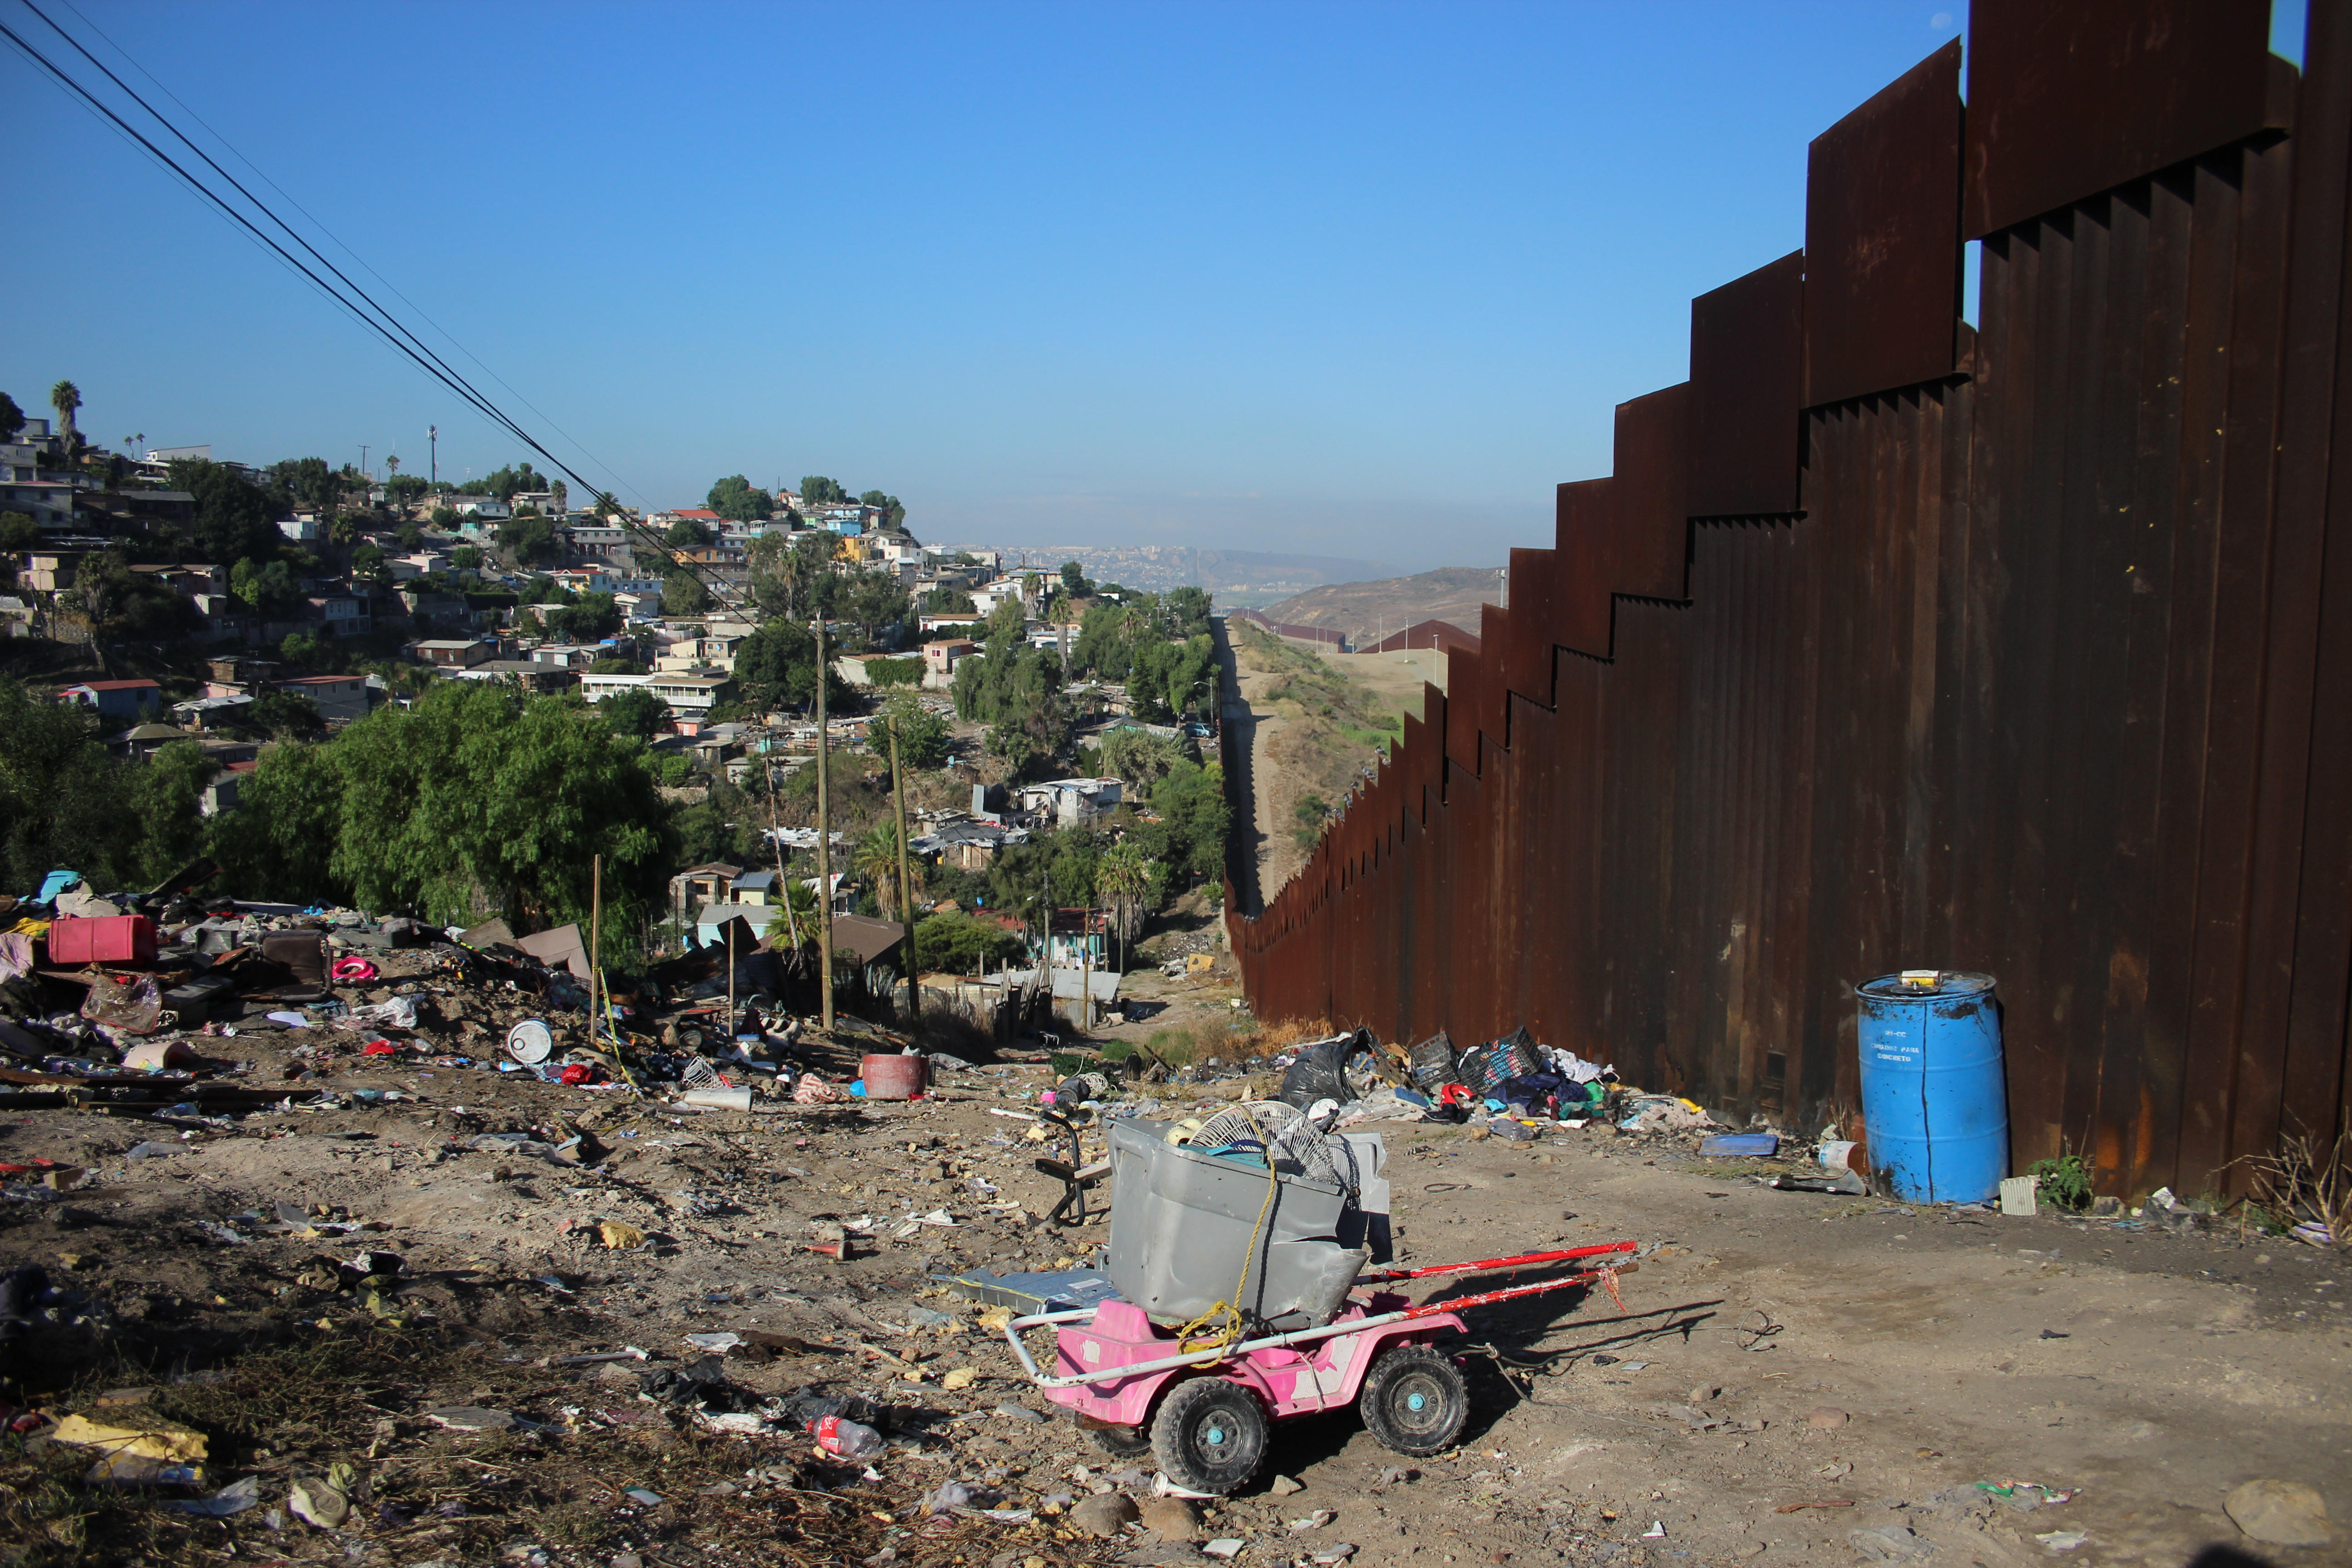
\includegraphics[width=0.85\linewidth,height=\textheight,keepaspectratio]{images/cap6libro2imagenA2026.JPG}

}

\caption{\label{fig-1}Condiciones de vida en el límite del muro
fronterizo de la colonia Libertad, Tijuana. Fotografía de la autora.}

\end{figure}%

La pobreza y desigualdad que les caracterizaba se contrastó con los
indicadores del \textcite{CONEVAL2012} a través de la ``Metodología para
la medición multidimensional de la pobreza en México''\footnote{Véase
  en:
  \ul{https://www.dof.gob.mx/nota\_detalle.php?codigo=5146940\&fecha=16/06/2010\#gsc.tab=0}}.
Este ejercicio tenía como finalidad, abonar a las estrategias de
conciliación a través de los avalúos de las propiedades. Los indicadores
que a continuación se presentan, permitieron identificar que, personas
del borde de la colonia Libertad vivían en condición de pobreza extrema:

\begin{enumerate}
\def\labelenumi{\alph{enumi})}
\item
  \textbf{Por ingresos}: el 40\% de las familias afectadas no contaban
  con recursos suficientes para adquirir los bienes y servicios que se
  requieren para satisfacer sus necesidades (alimentarias y no
  alimentarias).
\item
  \textbf{Por rezago educativo}. Los ``jefes de familia'' tenían como
  grado máximo de educación la secundaria.
\item
  \textbf{Calidad del espacio.} El 50\% de las propiedades en las que
  habitaban estas familias se construyeron de madera reciclada, con
  pisos de cemento y tierra.
\item
  \textbf{Acceso a servicios básicos.} Las familias que habitaban en
  Avenida Vía de la Juventud y Cañón Otay Parte Alta no tenían sistema
  de drenaje, agua potable y electrificación pública.
\item
  \textbf{Del contexto territorial}. El borde de la colonia libertad
  destacaba por ser un lugar no pavimentado; en el caso de los vecinos
  de la Avenida Vía de la Juventud, estos habitaban a un costado del
  canal de desagüe. Esa parte de la colonia Libertad se considerada
  ``zona de paso de polleros''. Durante el mes de mayo del 2023 se
  encontró un narco túnel en uno de los predios involucrados y semanas
  después el dueño fue asesinado a unas calles de su propiedad. Durante
  el mes de mayo y septiembre, dos posesionarios involucrados en el
  Proyecto fueron asesinados dentro de sus hogares por motivos
\end{enumerate}

\section*{Contexto histórico de la colonia
Libertad}\label{contexto-histuxf3rico-de-la-colonia-libertad}

\markright{Contexto histórico de la colonia Libertad}

Uno de los elementos que dio pie al nacimiento de la colonia Libertad
fue la ausencia de la intervención del gobierno. De acuerdo con los
datos obtenidos en el Acervo Histórico de Tijuana\footnote{Véase más en:
  \url{https://www.tijuana.gob.mx/ciudad/CiudadColonias.aspx}}, la
consolidación de esta colonia también responde a la intervención
militar. Las aportaciones del sociólogo Jorge A.
\textcite{Bustamante1990}, explican que la fundación de la colonia
Libertad nace del movimiento obrero de 1920, encabezado por los
trabajadores que participaron en la construcción y operación de los
servicios del viejo Hipódromo, espacio que albergó los primeros casinos
en esta ciudad fronteriza.

El crecimiento económico de Tijuana llamó la atención de personas
extranjeras, sin embargo la expansión económica de esta ciudad comenzó a
quedar en manos de empresarios y consumidores extranjeros. Bustamante
explica que el contraste era dramático: los clientes del lujoso casino
\emph{Agua Caliente} incluían estrellas de Hollywood, personajes de la
nobleza europea y exiliados de la primera guerra mundial. En cambio, los
mexicanos sólo habitaban los casinos para atender a esos extranjeros.

La gentrificación de la vieja Tijuana motivó a los trabajadores del
casino Foreign Club, Casino Agua Caliente, trabajadores del gremio de
choferes, trabajadores de la CROM y sindicalizados de la Liga
Nacionalista, a iniciar un movimiento bajo el lema: ``Quien vive en
Tijuana, en Tijuana debe trabajar''. En 1927 y 1928 comenzaron las
juntas sindicales, destacando la participación de Manuel Lerma, un
indígena Yaqui de Sonora.

Como parte de las iniciativas del movimiento, Manuel Lerma propuso que
los trabajadores se asentaran en las caballerizas del viejo hipódromo y
en los jacales de madera donde vivían los jinetes. Este lugar estaba
cercano a la antigua vía de ferrocarril, debajo de lo que ahora es la
colonia Libertad. Manuel Lerma ya había explorado la zona y sabía que
las caballerizas estaban abandonadas: ``los caballos vivían en mejores
condiciones de habitación que la mayoría de los trabajadores de Tijuana;
en construcciones techadas cerca del hipódromo''
\autocite[12]{Bustamante1990}.

Para ese entonces ya se había formado el Sindicato de Pequeños
Poseedores, teniendo como miembros a trabajadores que necesitaban de una
casa. En 1929 se registró la primera invasión: Manuel Lerma convenció a
veinte familias de tomar las caballerizas abandonadas, bajo la
justificación de que: ``los obreros tenían derecho a tomar estos
espacios porque ya los habían pagado con su trabajo y al estar en
abandono, tenían el derecho a ellas por haber contribuido con su
esfuerzo laboral'' \autocite[13]{Bustamante1990}. Al percatase de la
invasión, los dueños del hipódromo buscaron la forma de asegurar sus
propiedades, dando aviso al General Manuel Tapia, quien dio la orden de
desalojar a las familias que se habían apropiado de las caballerizas
abandonadas. Este evento provocó que el Sindicato de Pequeños Poseedores
fuera perseguido y buscado tanto en México como en EUA.

La persecución que sufría este grupo de trabajadores y sus familias
llamó la atención de otros obreros de Tijuana, quienes se sumaron a la
lucha. En esas condiciones se formó otra comisión para dirigirse con el
General Arturo Bernal, quien había sustituido al General Tapia. El
objetivo de esa comisión era lograr el apoyo del nuevo General para que
las familias del Sindicato de Pequeños Poseedores pudieran establecerse
en las viejas caballerizas. Arturo Bernal decidió apoyarlos poniendo fin
a la persecución.

Los Pequeños Poseedores organizaron expediciones a los basureros en
busca de material para construir sus viviendas. Domingo García, autor
del nombre ``Libertad'', sugirió contratar a un ingeniero para diseñar
el trazo de lo que sería la colonia. Bustamante puntualizó que, en ese
plano se dibujaron los lotes en figuras regulares de 16 x 45 metros, con
los nombres de las familias que los ocuparían.

\begin{figure}

\centering{

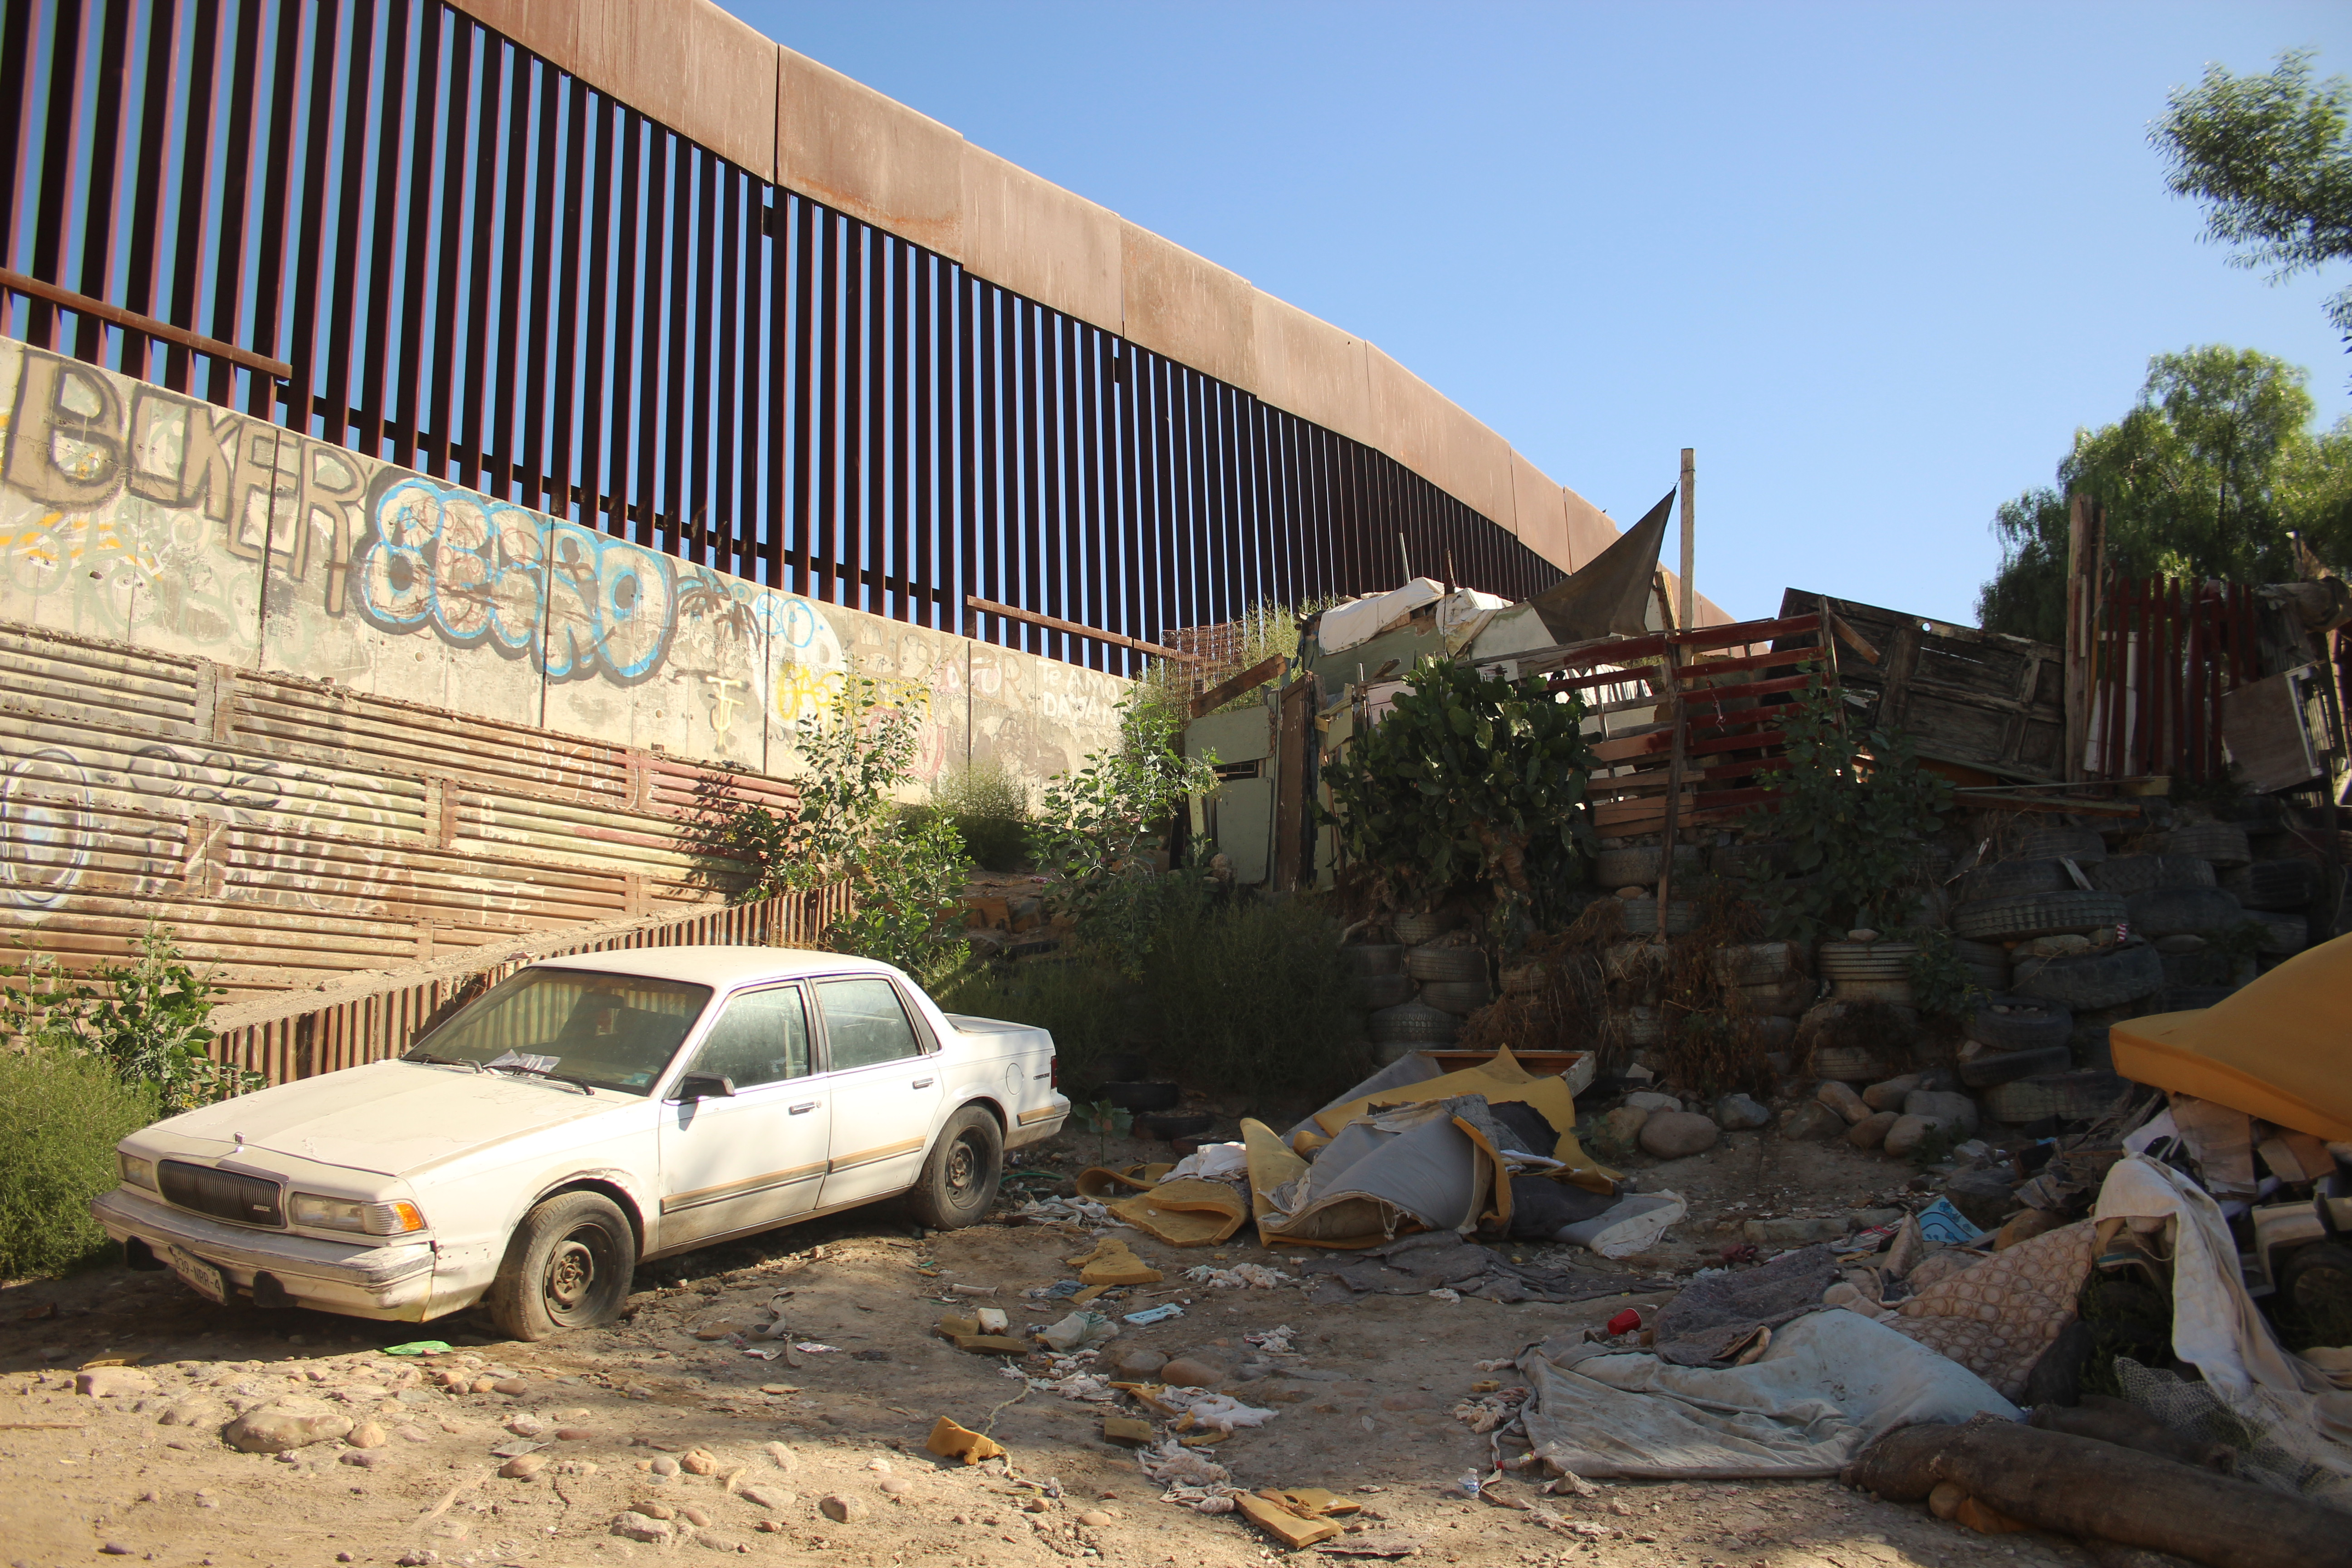
\includegraphics[width=0.85\linewidth,height=\textheight,keepaspectratio]{images/cap6libro2imagenB2026.JPG}

}

\caption{\label{fig-2}Vivienda autoconstruida y espacio habitacional
contiguo al muro de acero en el borde de la colonia Libertad. Fotografía
de la colección de la autora.}

\end{figure}%

La primera piedra se colocó en 1930. El dibujo del trazo, la alineación
de calles, la distribución de lotes, la construcción de viviendas y la
provisión de servicios fue iniciativa de particulares. La colonia
Libertad se expandió tras la llegada de mexicanos que fueron expulsados
de Estados Unidos durante la década de los treinta, familias que
decidieron asentarse en la colonia Libertad para mantenerse cerca de los
EUA.

Este pasaje histórico, autoría de Jorge \textcite{Bustamante1990}
continúa presente en la identidad de quienes viven en la colonia
Libertad, asumiéndose como personas que luchan. Sin embargo ese ímpetu
se disipa horizontalmente; el crecimiento de esta colonia fue desigual.
Esa desigualdad se alberga en un espacio segregado marcado por el muro
entre México y EUA, al que en este artículo se le denominará ``borde'',
espacio que continúa siendo el refugio de familias migrantes de escasos
recursos.

\section*{Apartado metodológico: la categoría borde y la importancia de
las historias de
vida}\label{apartado-metodoluxf3gico-la-categoruxeda-borde-y-la-importancia-de-las-historias-de-vida}

\markright{Apartado metodológico: la categoría borde y la importancia de
las historias de vida}

Las características espaciales y de interacción social que se
configuraron en el tramo de la colonia Libertad afectado por el
viaducto, deben entenderse desde la categoría \emph{borde}, un espacio
geográfico entre los límites de México y EUA. Lo particular de este
borde es que, este se impuso en la cotidianidad de sus habitantes, tras
la construcción del muro. Para comprender la propuesta central de este
artículo, dialogaré con las aportaciones de autores que brindan
interpretaciones de la categoría borde, entendido no solo como un
espacio geográfico que adquiere valor simbólico dependiendo del momento
histórico en el que se aborde, sino que va configurando un cúmulo de
experiencias que, en su mayoría, se desarrollan en contextos precarios.

Autores como Santiago Castro Gómez entienden la frontera/borde como:
``(\ldots) la zona intermedia, o el espacio entre dos mundos que surge
de un encuentro asimétrico (\ldots) forjando un sistema de jerarquías''
\autocite[12]{Castro2007}. Para Castro Gómez los bordes son el resultado
de los proyectos de modernidad, en los cuales las y los sujetos tienen a
reconfigurar sus dinámicas para resistir a los cambios y a la imposición
de nuevas jerarquías.

La socióloga Mariana Wagner explica que: ``(\ldots) la construcción de
bordes engendra un sentido en las personas de estar dentro o fuera de un
lugar (\ldots) los bordes concretizan el territorio y lo que estos
territorios significan. Los bordes señalan, y a la vez unen y contienen:
personas, ideas, prejuicios, formas de vida, bienes, sistemas,
etcétera'' \autocite[180]{Wagner2016}. Esta idea me lleva a retomar las
aportaciones de Walter Mignolo y el surgimiento de nuevas epistemologías
en los bordes, esto como resultado de los procesos de modernización que
construyen y albergan nuevas experiencias que se van interiorizando en
las personas, lenguajes, religiones y conocimientos. Mignolo resalta la
importancia ``(\ldots) no solamente de entender el borde como un espacio
geográfico, sino también como nuevas formas de política, subjetividades
y epistemes'' \autocite[315]{Mignolo2015}.

Esta idea dialoga con las experi encias de los habitantes que
permanecían/permanecen en el borde de la colonia Libertad. Personas que
configuraron sus subjetividades y cotidianidades conforme a los cambios
físicos del muro fronterizo, construyendo sus lógicas de pensamiento
desde un espacio lleno de desigualdad, pero que enaltecían por el hecho
de vivir a escasos metros del país vecino. Por ello la importancia de
registrar sus historias y sus vivencias, porque estas permitirán
comprender sus entramados sociales en diferentes momentos históricos.
Esto me lleva a retomar el trabajo del antropólogo Guillermo Alonso
Meneses, quien desarrolló los hechos que posibilitaron la construcción
del muro como se le conoce internacionalmente:

\begin{quote}
(\ldots) fue a finales de 1989 cuando los grupos de civiles, jubilados y
veteranos molestos por ``el caos'' que les causaba la migración en los
límites de San Diego, impulsaron la campaña \emph{``Lights up the
Border''.} La repercusión mediática que tuvo la acción de estos
vigilantes fronterizos y su odio hacia los mexicanos permitieron la
construcción del muro metálico con el fin de contener el flujo
migratorio. En 1991, la administración del entonces presidente de EUA,
George Herbert Walker Bush, comenzó a levantar una barda de acero entre
la playa de Tijuana y la Garita de San Ysidro; para su construcción se
utilizaron planchas metálicas de 2.4 metros de altura dispuestas en
vertical: plataformas viejas y oxidadas para helipuertos portátiles y
caminos que se ensamblaban, usadas en la guerra de Vietnam hasta 1975''
\autocite[265]{Meneses2023}.
\end{quote}

El muro que divide México de EUA no solo se trata de una barrera física
que impide el paso de migrantes, o que intenta ``proteger'' al país
vecino de agentes extraños\footnote{``(\ldots) el extraño desde el
  razonamiento de George Simmel es un modo de relación social o maneras
  de ser con otros (\ldots) la extrañeza no solo hace referencia a la
  exclusión que se construye desde la pobreza, sino que posibilita la
  construcción de figuras liminares, personas percibidas como intrusos,
  inferiores o marginales'' (\ldots) \autocite[PÁG]{Simmel2014a}.}
\autocite{Simmel2014a}. El muro como un dispositivo de control
\autocite{Foucault1976} construyó narrativas de distinción que reafirman
la supremacía blanca, su ideología de superioridad racial, social y
económica frente a los países del sur\footnote{Y aunque ``se acuse a los
  migrantes del medio rural de engrosar los cinturones de miseria en las
  ciudades, de quitarles empleo a los nativos, del deterioro de
  servicios públicos, etc. esta migración ha sido fundamental en el
  crecimiento y desarrollo de las ciudades mexicanas e incluso, del
  territorio americano'' \autocite{JesusArroyo2018}.}.

El análisis cualitativo de los datos contempló las historias de vida
como el recurso metodológico para abordar e identificar las
problemáticas y el sentir de las y los propietarios afectados. Sus
historias permitieron conocer e interpretar la realidad del borde de la
colonia Libertad, identificar el valor simbólico que construyó sus
subjetividades y cómo el muro fronterizo había influido en su
cotidianidad. Por esto se recurre a las aportaciones del sociólogo
Franco \textcite{Ferrarotti2012}, quien describe las historias de vida
como un método cualitativo que involucra la confianza y la construcción
de empatía entre interlocutores y el investigador:

\begin{quote}
es justo la comprensión profunda, y no sólo a la descripción de los
contornos externos, para lo que sirven las historias de vida (\ldots)
estas tienen un precio que obligan a ganarse la confianza de los
interlocutores (\ldots) ayudan a comprender que la persona que investiga
también es ``investigado'' \autocite[17]{Ferrarotti2012}.
\end{quote}

En tanto que, las historias de vida como método cualitativo brindan un
marco interpretativo que da sentido a las experiencias humanas. A través
de los relatos personales de las y los afectados por el Proyecto
Viaducto Elevando Tijuana, se logró entender sus acciones: su rechazo en
contra del proyecto o su interés por vender sus propiedades. Los datos
obtenidos en las historias de vida permitieron analizar cómo era su
relación con el borde de la colonia Libertad y el significado le daban a
su cotidianidad a partir de la transformación geográfica, física y
social de este espacio, todo en relación con el muro fronterizo.

Al identificar el valor histórico de los relatos, me permití continuar
con el registro de las historias, con el fin de preservar la memoria
colectiva de las personas que, involuntariamente, construyeron/habitaron
el borde de la colonia Libertad y que se vieron en la obligación de
vender sus hogares.

\begin{figure}

\centering{

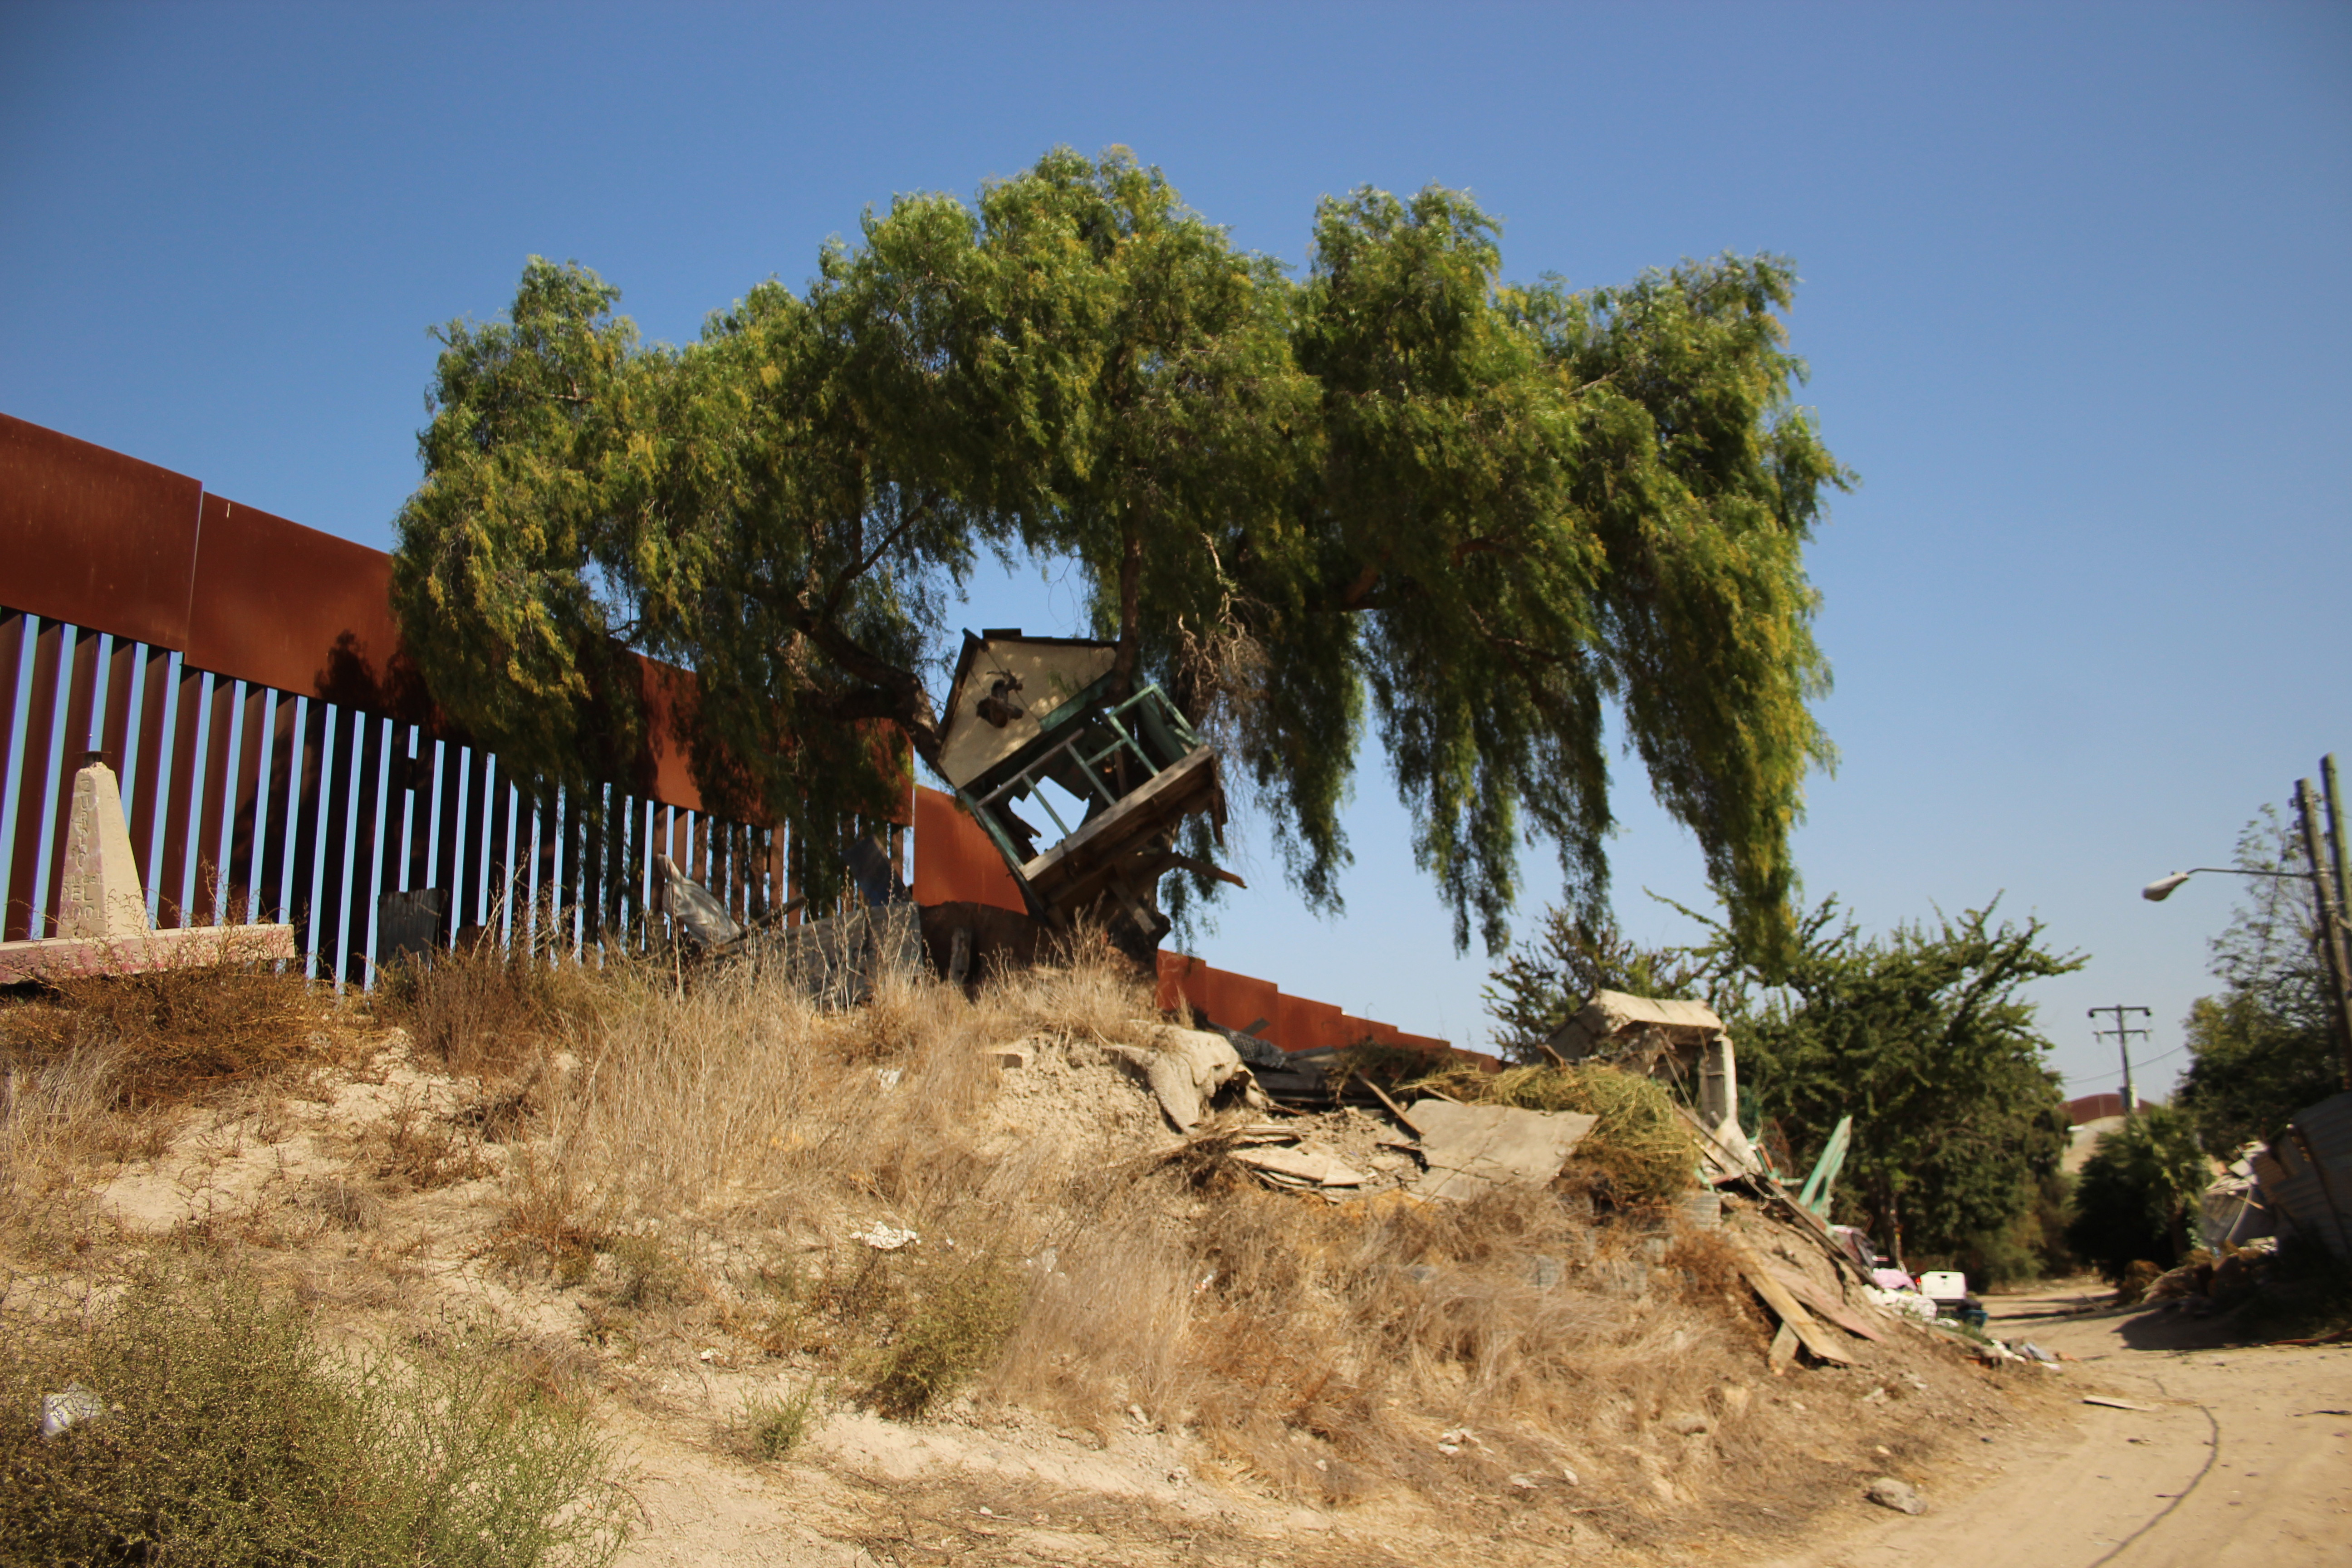
\includegraphics[width=0.85\linewidth,height=\textheight,keepaspectratio]{images/cap6libro2imagenC2026.JPG}

}

\caption{\label{fig-3}Transformación del paisaje y vestigios de la
memoria habitacional junto al cerco fronterizo. Fotografía de la
colección de la autora.}

\end{figure}%

\section*{La construcción del Borde de la colonia
Libertad}\label{la-construcciuxf3n-del-borde-de-la-colonia-libertad}

\markright{La construcción del Borde de la colonia Libertad}

Fueron los relatos de las y los propietarios los que permitieron
identificar que, antes del muro, el borde albergaba un sentimiento de
fraternidad entre los migrantes, los colonos de la Libertad y la policía
americana. También se identificó que los trabajos precarios\footnote{El
  debate en cuanto al concepto de trabajo precario se inició en Europa a
  principios de la década de 1970, mientras que en México el de
  precariedad laboral adquirió importancia en años recientes. Esta
  aparente falta de interés sobre el tema se debió a la heterogeneidad
  del mercado de trabajo en el país y a la asociación del empleo no
  asalariado con las naciones mencionadas, con el subempleo, la
  marginalidad, la informalidad y con el trabajo precario
  \autocite{Solis2014}.} como el del ``pollero'' surgió como una
alternativa de empleo, idea que se desarrollará más adelante. Para el
propietario ``Osvaldo'', vivir su infancia en el borde le permitió
habitar la frontera de forma lúdica, aunque también permitió identificar
la consolidación de las dinámicas comerciales de la colonia Libertad en
un espacio donde no había muro:

\begin{quote}
(\ldots) Allá donde vivimos nosotros ¿si te acuerdas?

\emph{Sí, antes de llegar a la glorieta del aeropuerto.}

Bueno pues cruzando del otro lado, cuando no había muro, antes allí
había un cerro, aunque los gringos ya lo rebajaron todo. Por allí se
estrelló una avioneta. Me acuerdo que, me tocó ver los cuerpos sin
cabeza ¡Se miraban bien feos!

\emph{Me imagino fue una sensación terrible\ldots{}}

Sí pues miré todos degollados. Esa avioneta (\ldots) como era de
aluminio la gente se llevó todo para venderlo. Haga de cuenta que en la
parte de abajo (Avenida vía de la Juventud) había un tianguis en donde
se vendían cosas para los polleros y para las personas que cruzaban,
pues allí se vendieron los restos de la avioneta. Eso fue en 1987, fue
noticia nacional.

\emph{¿La avioneta es el acontecimiento qué más recuerda?}

¡Hay bastantes historias!, sobre todo cuando antes se podía cruzar. Nos
pasábamos para jugar en el campo de fútbol que estaba del otro lado.
Todavía en 1989 pasamos el cerco para jugar y nos regresábamos cuando
nos cansábamos. A veces los migras nos miraban cruzar, pero sólo nos
saludaban y se acabó. No nos decían nada. Lo más que hacían los migras
eran tipos redadas: llegaban a ese tianguis que te digo y la gente se
salía corriendo, abandonando sus puestos. Aunque las redadas no eran
frecuentes.

\emph{¿Era peligroso vivir por este lado de la colonia?}

Fíjate que antes no había tanta violencia como ahorita. Lo que había
aquí era que asaltaban mucho a los polleros. Antes aquí vivía un tipo
que se llamaba ``Canelo'' ¡a ése cómo le gustaba asaltar a los
pollos\ldots hasta los golpeaba! Yo tenía como once años cuando vi que
los pollos se agarraban a balazos, hasta que mataron al Canelo. Aquí ser
pollero era un trabajo, pero ahora los polleros se sienten mucho. Si les
dices algo casi te matan. Mira, problemas de ese tipo siempre hubo. Pero
yo viví mi infancia muy feliz en este lugar (\ldots)

\begin{quote}
Fragmento de entrevista. Agosto 2023
\end{quote}
\end{quote}

Las historias de los vecinos afectados permitieron identificar que, el
borde fue adquiriendo vida por el fenómeno de la migración, esto llevó a
los habitantes de la colonia Libertad a emprender negocios enfocados en
facilitar el paso de las personas que cruzaban a los EUA a trabajar.
Este es el caso de ``Margarita'', quien formó su patrimonio vendiendo
comida a migrantes.

\begin{quote}
(\ldots) estaba yo acostada preguntándome qué haría porque cuando llegué
a Tijuana (\ldots) solo traía para que mis hijos no se murieran de
hambre. Cuando de repente pasó un señor diciendo: ¡pollo, pollo! Él
traía bolsitas con pollo del otro lado. En ese entonces la gente pasaba
por el cerro y pues traía cosas gringas para vender y ese señor traía
pollo. Le compré dos bolsitas que eran de seis libras cada una. Ese
mismo día saqué un bracero, puse el pollo en el carbón, compré verduras,
saqué mi mesita y así comencé. ¡En un ratito vendí todo el pollo!

\emph{¿Entonces había mucha gente por aquí?}

¡Huy sí! ¡Aquí hervía de gente? Al otro día traje más carne, más pollo.
Las mismas personas me ayudaban a sacar las cosas y a poner el puesto
porque tenían hambre. Era pura gente mexicana que quería ir del otro
lado y como no había muro pasaban rápido ¡montones que pasaban! No había
cerco, no había nada. Antes esto estaba lleno de gente. Ahora está solo.
En ese entonces había una arboleda en vez de muro ¡bonitos los árboles!
Venía la gente y se acostaba debajo de ellos. Pero después de que
pusieron el muro agarraron toda la calle y tumbaron los árboles. Ahora
nadie pasa, está solo.
\end{quote}

Las vivencias expresadas por las y los habitantes de la colonia Libertad
hacían referencia a las dinámicas que mantenían con EUA cuando ``no
había frontera'': se cruzaba para jugar béisbol en el campo, para lavar
ropa en el arroyo o para trabajar en San Diego. Todas y todos cruzaban;
la decisión de regresar a México dependía de la voluntad de cada persona
y no de un trámite legal. ``Juanita'', una mujer de 67 años narró la
forma en la que llegó a Tijuana y construyó su casa con la basura que
tiraban en el espacio donde ahora está el muro de acero.

\begin{quote}
\emph{``(\ldots) En la búsqueda de mejorar su calidad de vida, Juanita
migró con su marido de Nayarit a Tijuana en julio de 1969. Ella tenía 13
años cuando contrajo matrimonio con Gabriel, su difunto esposo, quien en
aquel entonces le llevaba ocho años. Al año siguiente comenzó su ciclo
de maternidad; sólo tuvo tres hijos.}

No recuerdo exactamente el año en que llegamos a Tijuana. Sólo sé que
fue en el mismo año que el hombre llegó a la luna. ¡Lo recuerdo porque
se hizo un alboroto!

\emph{Dice que Gabriel trabajaba como cargador de costales de azúcar y
desde ese año comenzaron a vivir en la colonia Libertad. Sin embargo y
tras el permiso de un conocido, Juanita, Gabriel y sus tres hijos
comenzaron a vivir frente al país vecino, en el borde, mucho antes de
que el territorio fuera dividido por un muro.}

En esa fecha llegamos con mi suegra, allí por el cañón Emiliano Zapata,
pero duramos poquito tiempo porque mis niños venían chiquitos y no
tenían dónde correr. Mi concuño era migrante y él fue quien compró aquí,
pero ya murió. Nos dijo que nos fuéramos a cuidar la casa y así
llegamos. Antes sólo había un cuartito y todo esto (señala con las
manos) estaba lleno de \emph{caiditos}\footnote{Invasores} \emph{todos
rascuachitos}\footnote{Forma coloquial para referirse a una persona,
  situación o contexto de marginación y pobreza.} como la casa. No
teníamos luz, no teníamos agua, no teníamos nada (\ldots) aquí estaba
todo destapado, no había divisiones, ni muros ¡hasta mis hijos jugaban
al otro lado ¡Primero echaron un muro de lámina y ahora ese muro! Antes
esto era un basurero y como pudimos se fue levantando la casita pa´
caber, porque no cabíamos: madera, lámina, cemento. Todo lo que
encontrábamos en la basura lo ocupamos para hacer nuestra casita
(\ldots)''

\begin{quote}
Fragmento de entrevista. Junio 2023
\end{quote}
\end{quote}

Florencia fue otra de las vecinas que llegó a vivir en el borde cuando
el territorio era ``solo uno''. La mujer reconoció que, pese a lo
solitario de la zona, durante la década de los 70´s pocas veces se veían
episodios de violencia, aunque era la pobreza era lo que delineó las
dinámicas de ella y de sus vecinos:

\begin{quote}
Cuando yo llegué nomás había una cerquita de alambre, pero podías pasar
con los gringos y nadie decía nada. Como allí tiraban los desperdicios
las fábricas y nosotros estábamos bien jodidos, mi esposo sacaba la
madera de la basura y comenzó a hacer una escalera para la casa. Pero
fíjese que antes no había tantos muertitos ni nada, había mucha paz. Yo
me acuerdo que, en ese entonces toda la gente salía a platicar en donde
ahora está el muro, ahora está vacío. Ni un alma (\ldots)

\begin{quote}
Fragmento de entrevista. Mayo 2023
\end{quote}
\end{quote}

\begin{figure}

\centering{

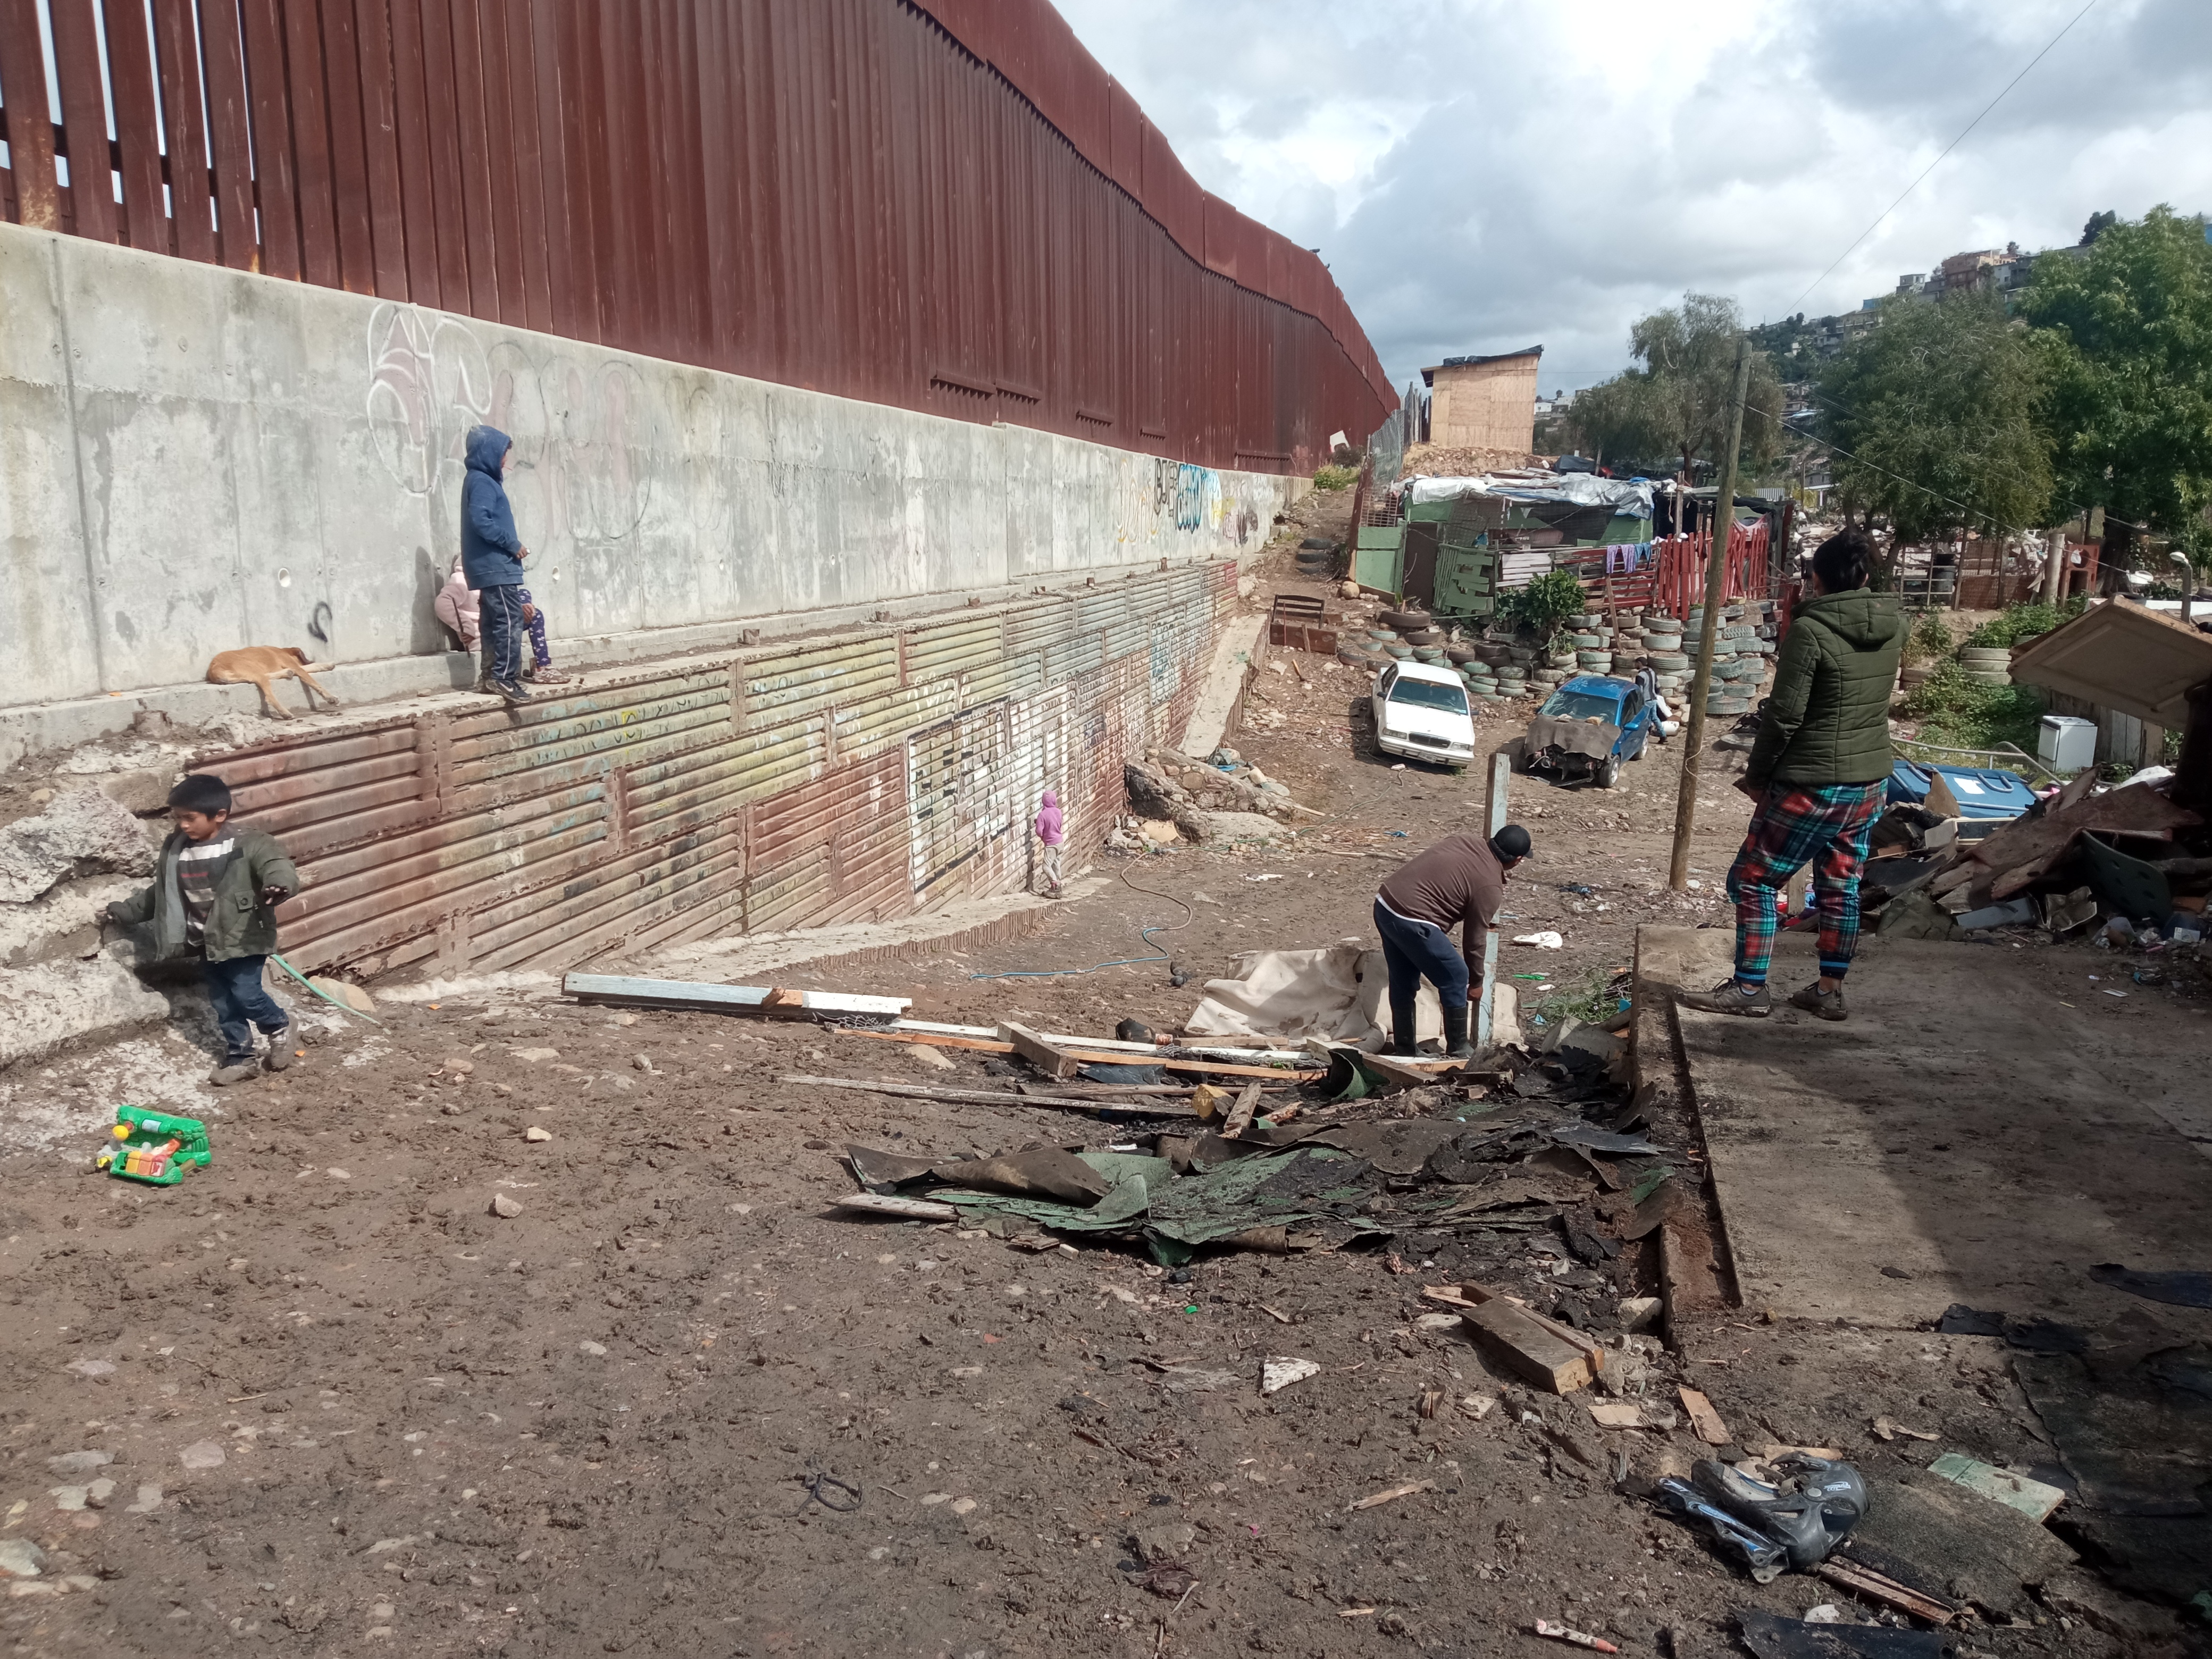
\includegraphics[width=0.85\linewidth,height=\textheight,keepaspectratio]{images/cap6libro2imagenD2026-01.jpg}

}

\caption{\label{fig-4}Convivencia en las inmediaciones del cerco
internacional en la colonia Libertad. Fotografía de la colección de la
autora.}

\end{figure}%

\section*{Patrimonio irregular: violencia e
incertidumbre}\label{patrimonio-irregular-violencia-e-incertidumbre}

\markright{Patrimonio irregular: violencia e incertidumbre}

Las y los vecinos explican que en el borde de la Libertad no pasaba
mucho y que la intervención del Gobierno Local y Federal sólo era
visible en campañas electorales. Retomando los aportes del sociólogo
Jorge Bustamante, él explica que un elemento muy significativo del
nacimiento de la colonia Libertad respondió a la ausencia y falta de
intervención del Gobierno: ``(\ldots) tanto el trazo y alineamiento de
las calles, la distribución de los lotes, la construcción de las
viviendas y la provisión más elemental de servicios, fueron iniciativa y
logro de particulares organizados para beneficio de su propia comunidad.
No hubo''decisiones de arriba'' en la creación de la colonia. Fueron la
determinación, la solidaridad y la conciencia nacionalista de ``los de
abajo'', los ingredientes principales de la colonia Libertad''
\autocite[13]{Bustamante1990}.

En tanto que los hallazgos del sociólogo Jorge Negrete
\autocite{Mata1993}, puntualizan que, entre la década de 1950 y 1970 el
crecimiento de Tijuana está catalogado como uno de los más acelerados
del país. En veinte años, esta ciudad definió su perfil socioeconómico a
partir de la predominancia del comercio, los servicios turísticos y la
consolidación de una industria propia. Su cercanía con EUA le permitió
desarrollar empresas trasnacionales en donde predomina la industria
maquiladora, la cual dirigió el proceso de industrialización de Tijuana,
representando una oportunidad laboral para personas de todo el país.

La toma de decisiones y la politización del espacio por parte de los
gobiernos en turno\footnote{Un ejemplo de estas políticas fueron las
  iniciativas del exgobernador Xicoténcatl Leyva Mortera, sexenio en el
  que proliferaron las invasiones. El eslogan de campaña del gobernador
  era, ``un lote para cada familia humilde \autocite{Mata1993}.} fueron
factores que endurecieron la desigualdad social en Tijuana. Continuando
con las aportaciones de Jorge Negrete, este explica que Tijuana se
construyó en medio de muchos problemas vinculados con la propiedad del
suelo urbano: invasiones propiciadas o permitidas por el gobierno,
rescate de zonas invadidas, reubicación, desalojos o permutas de suelo
invadido por terrenos habilitados \autocite{Mata1993}. Este fue el
motivo por el que los propietarios afectados en el viaducto temían de
una ``expropiación'', porque históricamente la expropiación en Tijuana
ha sido un instrumento político que ha permitido el reordenamiento
urbano de la ciudad. En tanto que su condición como poseedores sembraba
miedo e incertidumbre sobre su porvenir.

La segregación espacial del borde se agudizó con el paso migratorio.
Para autores como Ariel Espino, las divisiones y segregaciones responden
a la lógica del sistema y a los resultados del libre mercado: ``los
desarrolladores construyen vecindarios de distintos niveles económicos y
los compradores se distribuyen en el espacio urbano según sus ingresos''
\autocite{Mendez2018}. Por ello el borde de la colonia Libertad tiene
las características de un territorio segregado, en el que aún
habitan/habitaban familias con índice de pobreza extrema.
Paradójicamente las familias más pobres de este lugar vivían a escasos
metros del país más rico del mundo.

La resignación de las y los propietarios les llevó a familiarizarse con
el equipo de liberación de vía, permitiendo las primeras negociaciones;
las personas en condición de pobreza fueron las primeras en conciliar.
Aunque las y los propietarios reconocían que el Gobierno Federal les
estaba ``pagando bien'', al entablar conversaciones más profundas y tras
un sinfín de visitas, se identificó que los motivos por los que no
querían irse del lugar, pese a la inseguridad y la violencia que se
vivía por ser ``zona de polleros'', era que la cercanía con EUA les daba
``estatus'', en comparación con otras colonias populares de Tijuana,
como ``El Florido'':

\begin{quote}
(\ldots) yo digo que la ventaja de estar aquí, en la Libertad, pues
casi, casi estamos bien céntricos y cerca de los gringos. Y fíjate qué
bueno que estamos hablando de esto. ¡Qué caro está Tijuana! ¡Yo me estoy
quebrando la cabeza! Duermo bien tarde, estoy revisando lugares y casas.
Yo me digo ¡No me va a alcanzar, está caro! ¡No te puedes imaginar!
¿Dónde voy a encontrar un lugar así de cerquita de los United States
(\ldots)

\begin{quote}
Fragmento de entrevista de ``Emanuel'', mayo 2023
\end{quote}
\end{quote}

Las y los propietarios afectados de escasos recursos, quienes nunca
habían cruzado a los EUA y mucho menos contaban con una Visa, enaltecían
vivir frente al país más poderoso del mundo, lo que les permitía
construir un sentimiento de orgullo por vivir en el borde de la colonia
Libertad: se sentían privilegiados aunque hubiera un muro de por medio.
En cambio, otros propietarios en la misma situación económica habían
cambiado de parecer cuando las dinámicas de violencia en la zona
repercutieron en su cotidianidad, pero su pobreza no les permitía
mudarse a otro lugar y desconocían la existencia de apoyos
institucionales. Esto se identificó en dos casos de mujeres; ``Rocío''
de 60 años que había perdido la vista a consecuencia de la diabetes,
explicaba que la ubicación de su casa era el factor que impedía a las
instituciones sociales de Tijuana hacer enlaces en materia de política
social:

\begin{quote}
\emph{(\ldots) - ¿Quiere hablar sobre la muerte de su esposo?}

Sí, no hay problema. Ya pasó.

\emph{¿Quiere contar en dónde falleció su esposo?}

Allá adelantito, por donde vive doña ``Rosita'', por ese rumbo. Lo
balacearon. No se supo el por qué. Ya ve que, si uno no tiene dinero, no
investigan. Nada más lo balacearon y no aguantó los balazos por eso
falleció. Un vecino vino a hablarle a mi hija pues porque yo no podía
salir y vinieron a avisarle para que le hablaran a la ambulancia. Cuando
la ambulancia llegó se lo llevaron vivo, pero dicen que en el hospital
falleció.

\emph{¿Entonces nunca supieron quién fue el responsable?}

No, nunca supimos. Y pues no queremos porque ya ve que es un área
peligrosa. Vale más vivir así, en paz, sin saber quién fue.

\emph{El muro que divide la frontera con Estados Unidos forma parte del
patio de ``Rocío''. Es curioso ver la facilidad con la que sus perritos
y gallinas atraviesan el muro y cruzan al país vecino en busca de comida
o sombra para echarse, pero sus animalitos siempre regresan. La casa de
``Rocío'' también está a unos pasos del lugar donde se encontró un narco
túnel. La mujer explica que la cotidianidad alrededor de su casa siempre
ha involucrado el paso de migrantes, aunque dice que con el paso del
tiempo las cosas han empeorado.}

\emph{¿Tiene miedo de vivir aquí?}

No, ya me acostumbré (ríe). Pero ya uno qué puede hacer, más que oír y
callar. Encerrarse más que nada. Mis perritos me avisan cuando pasa
alguien, son bien escandalosos por eso sé cuándo alguien pasa afuera de
la casa. Luego pasan corriendo por el techo. Son los migrantes, los
polleros. Yo ni salgo (\ldots)

\begin{quote}
Fragmento de entrevista. Junio 2023
\end{quote}
\end{quote}

Para propietarias como ``Paola'', la construcción del segundo piso
representó una posibilidad de mejorar la calidad de vida de su familia,
sobre todo tras la pérdida de uno de sus hijos; un joven de 21 años
asesinado a la misma altura donde el esposo de ``Rocío'' fue baleado, lo
que permite identificar las dinámicas de violencia que se desprenden en
el borde por ser paso de migrantes. Con este argumento no busco
criminalizar a las personas que buscan llegar a los EUA, esto debe ser
entendido como el resultado de las políticas migratorias americanas que
criminalizan el territorio mexicano:

\begin{quote}
\emph{Paola explica que tiene más de 20 años viviendo en el borde de la
colonia Libertad con su esposo y dos hijos. Su casa es de madera y el
piso es de tierra; no tiene sistema de agua potable/ drenaje y uno de
sus vecinos le pasa luz. La primera vez que ella se acercó con el equipo
para conciliar, fue porque ya no quería vivir en el borde de la
Libertad. Paola cuenta que su casa fue un regalo de su tío. Pero no
tiene escrituras. Su condición de posesionaria le causaba incertidumbre
porque no tenía como demostrar que aquella era su casa. Lo único que
pedía es que no se le dejara en la calle y que, de ser posible, se le
apoyara para vivir en otra colonia.}

Esta colonia es peligrosa. Yo ya no quisiera vivir en este lugar. En
octubre del año pasado (2022) me mataron a mi hijo, aquí a la vuelta de
mi casa (solloza). A diario matan gente aquí. Esta colonia se ha vuelto
peligrosa. Si ustedes pueden ayudarme a irme de aquí, estaría mejor
(\ldots).

\begin{quote}
Fragmento de diario de campo. Febrero 2023
\end{quote}
\end{quote}

La construcción del viaducto permitió observar la facilidad con la que,
espacios como el borde, podían ser invadidos, incluso podían ser
arrendados por los mismos invasores por una cuota mensual de mil pesos
mexicanos (48 dólares). La mayoría de estos espacios eran ocupados por
los polleros, lo que desataba una lucha de territorio por los predios
deshabitados. Este señalamiento se pudo identificar con el caso de un
invasor de nombre ``Javier'':

\begin{quote}
``Javier'' se mostraba preocupado. No tiene escrituras y no puede
conciliar. Por ese motivo se le volvió a visitar, para informarle que,
si él lo deseaba, se le podía buscar un espacio temporal en un albergue
en lo que encontraba un lugar para vivir con su esposa e hija. Javier
insiste en permanecer en el borde, incluso ``nos ha pedido permiso''
para invadir el predio de a lado.*

Yo les quería preguntar si me puedo mover para la siguiente casa. Allí
no vive nadie. Me puedo mover un rato en lo que encuentro dónde ir.

\emph{``No Javier, ésa también se va a tirar y por allí va a pasar el
puente'', le explicó el abogado.}

¿Puedo levantar un cuarto por allá? Jaime señaló otro predio, lugar que
también estaba afectado por el Viaducto.

\emph{``No Jaime, por todo este lugar no puedes levantar nada. Todo esto
se va a ir. Todo se va a demoler'', contestó nuevamente el abogado.}

Es que no me quiero ir a un albergue. Nos da miedo que el DIF nos quiera
quitar a la niña (\ldots)

\begin{quote}
Fragmento de entrevista. Agosto 2023
\end{quote}
\end{quote}

Semanas después de aquella visita, Javier y su esposa fueron asesinados
con un arma de fuego. Tras el deceso de Jaime se descubrió que él
ocupaba el predio para esconder a migrantes y el incidente fue un ajuste
de cuentas con los polleros de la zona. Vecinos explicaron que la niña
de 9 años salió huyendo y fueron los mismos vecinos quienes la apoyaron
por un par de días. Al no contar con más familiares, la pequeña fue
trasladada al DIF estatal de Baja California.

\begin{figure}

\centering{

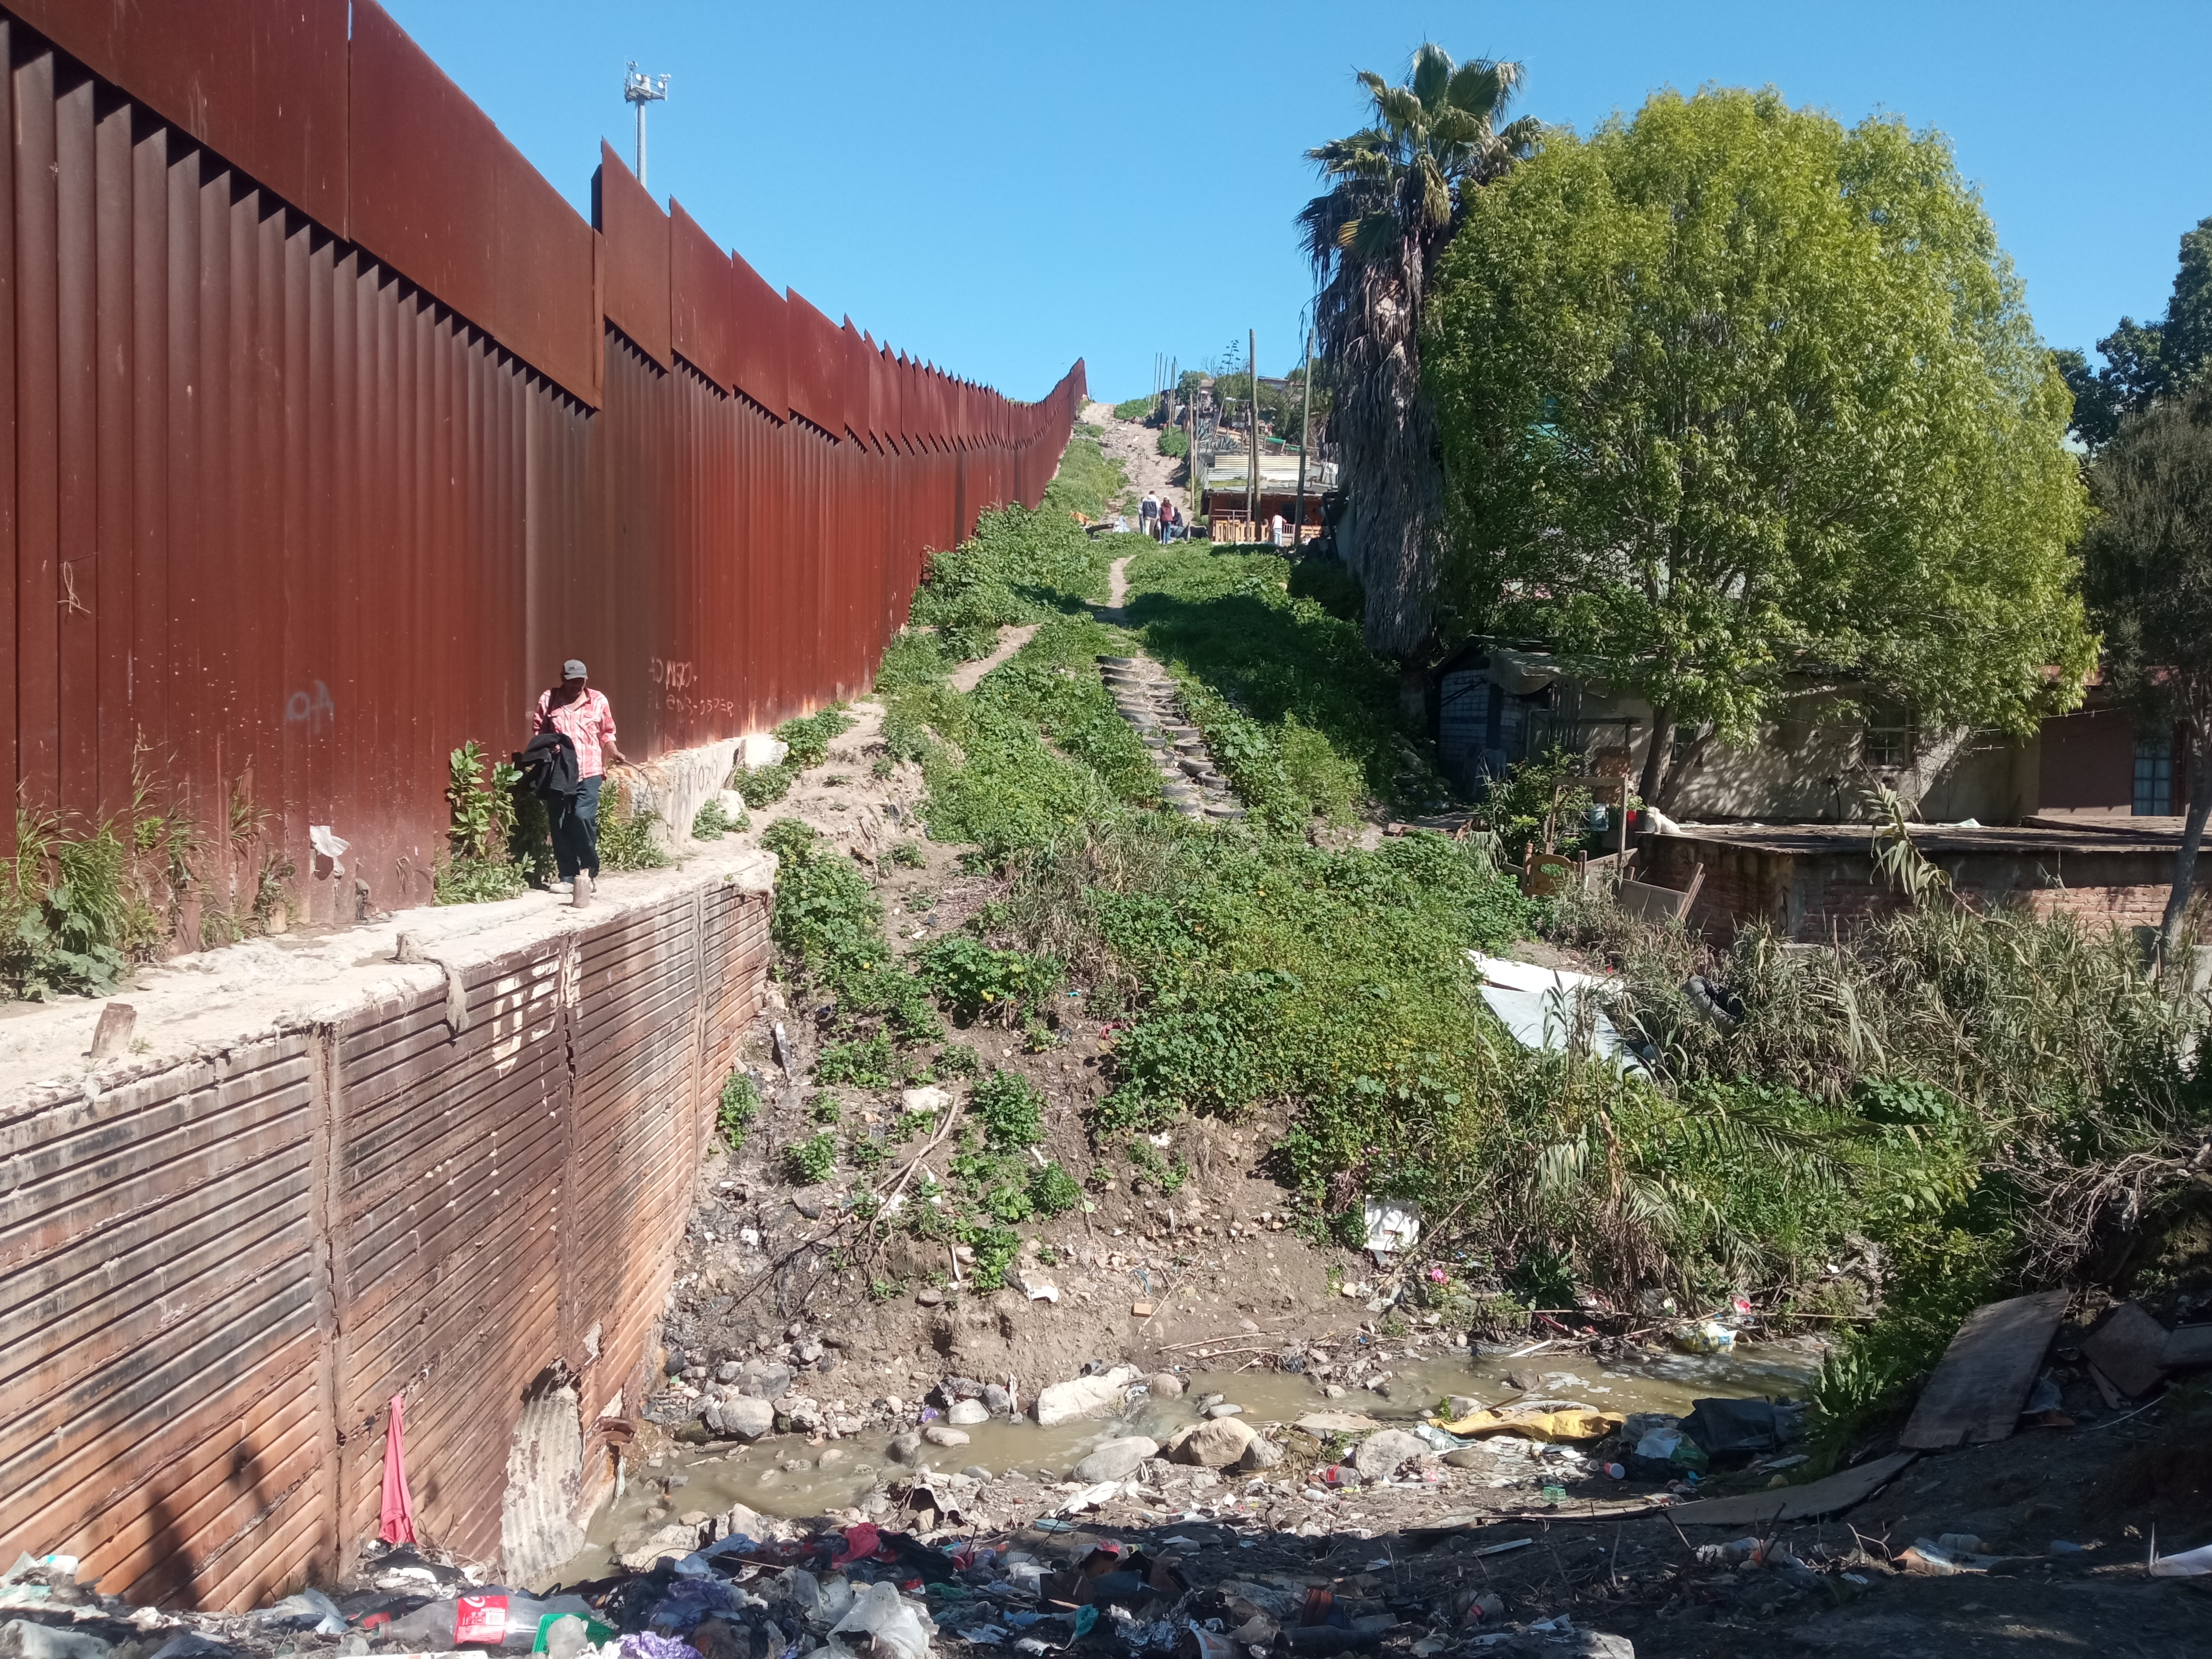
\includegraphics[width=0.85\linewidth,height=\textheight,keepaspectratio]{images/cap6libro2imagenE2026-01.jpg}

}

\caption{\label{fig-5}El borde de la colonia Libertad. Fotografía de la
colección de la autora.}

\end{figure}%

\section*{Un borde de polleros}\label{un-borde-de-polleros}

\markright{Un borde de polleros}

Al ser el borde de la colonia Libertad un espacio segregado, resultado
de la falta de apoyos por parte del gobierno local, se observó que desde
la consolidación de la colonia, sus habitantes emprendieron una serie de
trabajos precarios \autocite{Solis2014} que resignificarían este lugar
como ``el paso de migrantes''. Los vecinos cuentan que hasta la década
de los ochenta era común la instalación de un tianguis en el que se
vendía comida, ropa, cobijas y demás artículos para las personas que
cruzaban de forma ilegal a EUA. También era común que los vecinos
pusieran en marcha un tipo de servicio de guía para migrantes, en donde
se les ofrecía un método de ``hospedaje, cruce y acompañamiento'',
actividades destinadas a los ``polleros''. Las charlas coloquiales
permitieron comprender que las personas de la colonia Libertad forjaron
su patrimonio cruzando a migrantes:

\begin{quote}
(\ldots) pero al poner el muro cambió todo. No te imaginas la multitud
de gente que antes había. La forma de vivir allí era siendo pollero.
Allá era la mera mata para cruzar. Todos eran polleros, te puedo decir
de los que viven en la Libertad quienes eran polleros. Pero antes ese
trabajo no era malo, porque ser pollero era cruzar a la gente y
llevarlos a su destino, como un chofer, aunque no cobraban tanto dinero
como ahora (\ldots) Llevaban a la gente en camionetas. Los polleros
antes te cuidaban, te llevaban a tu destino. Ahora te violan, te
abandonan, te roban. Pero eso comenzó a pasar cuando pusieron el muro y
comenzó la venta de droga en la Libertad (\ldots)

\begin{quote}
Fragmento de entrevista. La ``licenciada''. Junio, 2023
\end{quote}
\end{quote}

Sin embargo, la labor del pollero se criminalizó tras la creciente
vigilancia de la frontera. Autores como Alfredo Jáuregui y Ma. de Jesús
Ávila explican que a mediados de 1990 y como parte de una estrategia
nacional estadounidense: ``la vigilancia de la frontera se endureció con
más agentes de la patrulla fronteriza (\emph{U.S. Custom and Border
Protection, CBP}), con la construcción de muros y bardas en los puntos
de cruce tradicionales que no sólo prevenían la entrada de migrantes
indocumentados, sino que facilitaban su aprehensión'' (2017).

Los propietarios reconocieron que ser pollero no era malo, porque era de
las pocas fuentes de empleo en la colonia, sobre todo en las zonas de
Cañón Zapata y Avenida Vía de la Juventud \autocite{LopezReyes2021}. Las
dificultades comenzaron cuando esta actividad resultó atractiva para los
carteles mexicanos del narcotráfico, ``quienes descubrieron en ella una
fuente alterna de financiamiento en la que se aprovechaban de las rutas
de paso de migrantes para el trasiego de drogas'' (Jáuregui, Ávila
2017). Los vecinos de la Libertad reconocen que fue el fenómeno del
narcotráfico el hecho que intensificó el peligro para la colonia y para
los migrantes, quienes aún son víctimas de secuestros, extorsiones, o
que son usados como mulas para el cruce de droga a Estados Unidos. La
falta de empleo para las personas de escasos recursos que vivían/viven
en el borde es lo que les lleva a buscar actividades que ponen en riesgo
su vida.

La intervención del crimen organizado con el cruce ilegal de personas
obligó a muchos residentes del borde de la colonia Libertad a retirarse
del negocio de polleros. Aunque la construcción del muro a partir de
1995 y reforzado en el año 2006\footnote{Una división artificial de
  construcción del otro, en un muro metálico de contención de tres
  metros de altura, en un estado de oxidación constante, construido
  desde 1995 y reforzado después de 2005, que tiene 1, 123 km emanado
  del mar de Playas de Tijuana, circundando toda la frontera hasta
  llegar a la Playa de Bagdad en Tamaulipas \autocite{LopezReyes2021}.}
no fue un impedimento para que este espacio dejara de capitalizarse.
Aunque, y de acuerdo con las declaraciones de propietarios, los polleros
de ahora son ``mafiosos y matones'', personas ajenas a la colonia.

\section*{Conclusiones}\label{conclusiones-2}

\markright{Conclusiones}

Informar a una persona que ``debía vender su casa''\footnote{Este
  siempre fue el argumento de los vecinos cuando se les visitaba.} no
fue una tarea fácil, pero era un mandato federal y se tenía que hacer.
Escuchar y analizar los reclamos permitió comprender que la
incertidumbre de los 176 afectados respondía más a factores emocionales
porque ellos se construyeron como personas fronterizas a la par del
muro; tenían miedo no solo de de volver a comenzar una vida en un nuevo
lugar, sino de vivir lejos de los EUA.

El olvido institucional que históricamente ha marcó a los habitantes del
borde de la Libertad está presente en sus vivencias, las cuales se
encarnan en un contexto de pobreza y de violencia, donde participa el
crimen organizado. En el borde hay asesinatos, violaciones, asaltos,
invasiones a predios por polleros, venta de drogas y cruce ilegal de
personas. Por ello, en ocasiones, socializar el viaducto terminaba
convirtiéndose en un tipo de terapia psicológica, en donde el
propietario narraba sus experiencias y su hartazgo por vivir en una zona
peligrosa pero que les costaba dejar. Además de que, identificaban lo
``absurdo'' que resultaba la construcción de un segundo piso en Tijuana,
cuando era evidente la falta de políticas públicas en el borde de la
Libertad.

La única vez que vieron actuando de forma tajante al Gobierno Federal,
fue cuando se les informó que tenían que vender sus propiedades y que si
no conciliaban con el equipo encargado de liberar la vía, tenían que
hacerlo directamente con la SEDENA. Ningún propietario quiso conciliar
con soldados.

Genuinamente y para lograr la conciliación, se puso en marcha un método
de análisis biográfico que estableció las estrategias de negociación.
Después de cada visita en campo, se sugirió a los cuatro abogados
platicar sobre lo que habían visto: la percepción de los propietarios,
quejas, sugerencias, miedos o amenazas. Aunque las charlas se tornaban
coloquiales, dentro de las conversaciones se confeccionaron las tácticas
para abordar a cada propietario, prestando atención al valor emocional
que las personas sentían por el hecho de no querer vender sus
propiedades.

\begin{figure}

\centering{

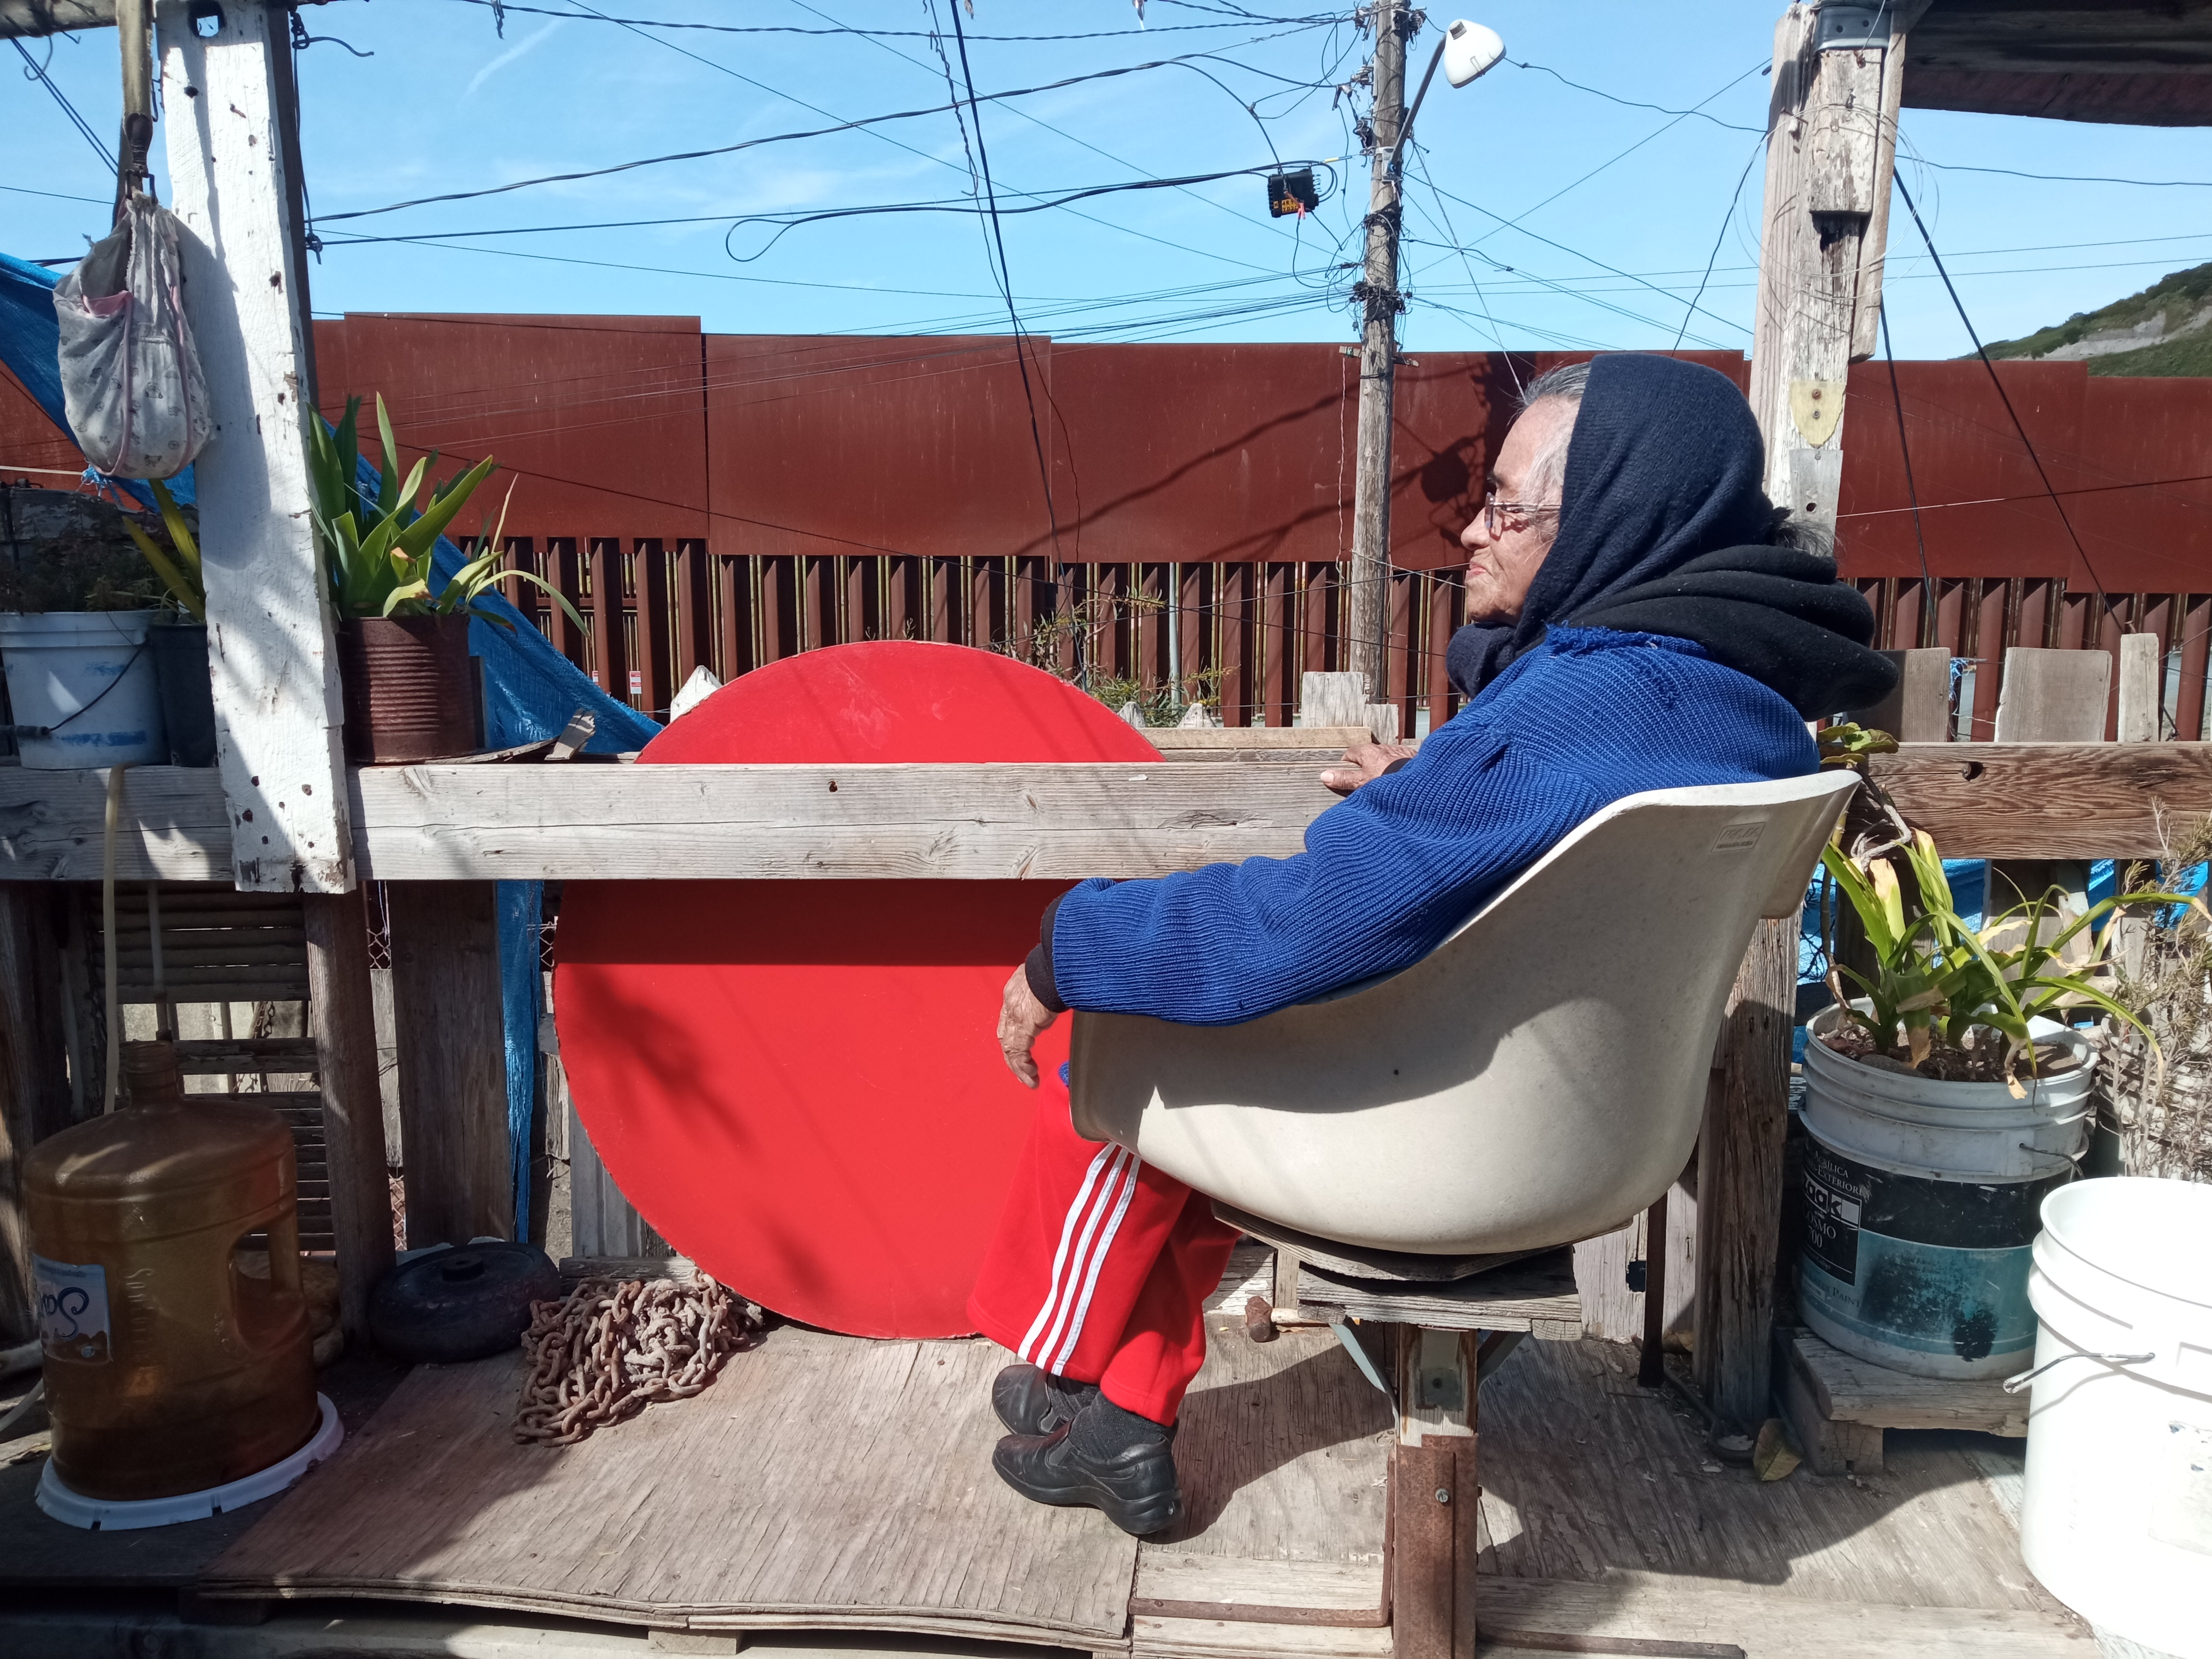
\includegraphics[width=0.85\linewidth,height=\textheight,keepaspectratio]{images/cap6libro2imagenG2026.jpg}

}

\caption{\label{fig-6}La vida cotidiana en el borde de la colonia
Libertad}

\end{figure}%

Durante los recorridos de socialización y reconocimiento del lugar, los
propietarios explicaron que algunos de sus familiares habían sido
asesinados a unos pasos de sus hogares; que los asaltos, levantones,
venta de drogas y violaciones les hacían reformular sus horarios fuera
de casa. Aunque a lo largo del articulo no se profundizó en los eventos
que marcaron al equipo de liberación de vía en los trabajos de campo, me
permito mencionar (solo como un indicador para enfatizar en la violencia
que se vivía en el borde) que en un lapso de seis meses se presenció el
descubrimiento de un narco túnel en una casa afectada por el viaducto y
se nos informó de dos asesinatos de posesionarios con quienes se había
entablado un lazo de amistad. Por ello se advertía al equipo sobre tener
cuidado en el borde y evitar transitarlo después de las 5 de la tarde.

Las historias de vida permiten conectar escenarios, tiempos y contextos
que son necesarios no solo con fines teórico-metodológicos, sino como un
ejercicio que documenta procesos históricos locales. En el caso del
viaducto, las historias de vida permitieron tipificar estrategias de
socialización para abordar a cada uno de los propietarios afectados,
conforme a sus necesidades y contextos. Probablemente ése fue el éxito
de la conciliación en el proyecto Viaducto Elevado Tijuana: dejarse
llevar por la intuición y por la narrativa de los propietarios, dándoles
tiempo, siendo empáticos y pacientes. Dando agencia a sus
recomendaciones y peticiones rescatadas de las historias de vida.

Finalmente, el ejercicio de documentar las historias de algunos
propietarios afectados no sólo buscaba interpretar el contexto social/
espacial del borde; también se cuestionan los cambios que la ciudad
tendrá después de la construcción del viaducto y que, de acuerdo con las
características del proyecto, las modificaciones en la colonia son
irreversibles. Aunque la narrativa del gobierno federal enaltece la
modernidad, el crecimiento económico y el mejoramiento urbano de
Tijuana, la intención de registrar las historias de ``un antes y un
después'' este artículo busca ser una herramienta para recordar quiénes
fueron las personas que habitaron el borde de la Libertad y la forma en
la que un megaproyecto incidió en su cotidianidad.

\printbibliography[heading=subbibliography, title={Referencias Bibliográficas}]

\bookmarksetup{startatroot}

\chapter{El diseño de las políticas públicas a partir de las
observaciones flotantes en los espacios públicos de Ixtapaluca, Estado
de
México}\label{el-diseuxf1o-de-las-poluxedticas-puxfablicas-a-partir-de-las-observaciones-flotantes-en-los-espacios-puxfablicos-de-ixtapaluca-estado-de-muxe9xico}

\addtocontents{toc}{\protect\hspace{1.5em} Edgar Flores Gómez \par}
\markboth{Observación Flotante en Diseño de Políticas Públicas}{}

\begin{flushright}
\Large Edgar Flores Gómez \footnote{Licenciado en Sociología por la Universidad Autónoma Metropolitana (Unidad Xochimilco). Su formación de posgrado incluye la especialidad en Género en Educación por la Universidad Pedagógica Nacional (Unidad Ajusco) y la maestría en Práctica Docente por la Universidad Autónoma del Estado de México. Contacto: \href{e.flores@correo.ler.uam.mx}{e.flores@correo.ler.uam.mx}}
\end{flushright}

\section*{Introducción}\label{introducciuxf3n-5}

\markright{Introducción}

En este texto destaco el trabajo etnográfico y sus implicaciones en el
diseño de las políticas públicas, específicamente, relativas al espacio
público, teniendo como referente el trabajo empírico que realicé en el
municipio de Ixtapaluca, Estado de México. De tal manera, desde la
antropología urbana y acudiendo a la técnica para recopilar información
empírica, la observación flotante, menciono que dentro de sus
principales fortalezas, está la posibilidad de aproximar al científico
social a la cotidianidad y actores que indaga. En el mismo sentido, la
observación flotante, por su ``espontaneidad'', está relacionada con la
``objetividad'' y ``neutralidad''. En resumen, acudir a la observación
flotante, encierra la posibilidad de emplear una técnica para recopilar
información durante el trabajo etnográfico que es flexible, cambiante,
la cual se adapta, se moldea y se aproxima a cada situación que se
presenta de forma espontánea en el contexto de indagación empírica de
quien investiga, en mi caso y como etnógrafo urbano, me permito abrir un
paréntesis, para mencionar que la redacción de este texto es en primera
persona, fundamentalmente porque se trata de un trabajo etnográfico
realizado de forma individual, partiendo de los principios de
objetividad y neutralidad que se requieren para realizar investigación
científica social.

Respecto al diseño de las políticas públicas, hago la precisión de que
no es mi objetivo verificar determinada política relativa a los espacios
públicos en el municipio de Ixtapaluca; no obstante, señalo que a partir
de una búsqueda en la página del Ayuntamiento Constitucional de
Ixtapaluca, recabé el ``Plan de desarrollo municipal Ixtapaluca:
Ayuntamiento 2022-2024'', información que sirve de punto de partida y
que compartiré más adelante. Igualmente, reconozco que existe un vínculo
indivisible en el diseño de las políticas públicas, particularmente al
estar relacionadas con procesos socioculturales que se presentan en la
cotidianidad. Es así que se propone el diseño de políticas públicas que
rompan con lo convencional, que trasciendan a sus concepciones comunes,
en donde los ejercicios etnográficos, son relevantes por su cercanía con
los acontecimientos y los actores en el escenario de su cotidianidad.

En cuanto a los contextos en los que realicé las observaciones
flotantes, adelanto que las llevé a cabo en cuatro espacios públicos del
municipio de Ixtapaluca, Estado de México, ubicado en la zona
sur-oriente de la Zona Metropolitana del Valle de México e,
históricamente, había sido identificado como un lugar transitorio entre
la Ciudad de México y el estado de Puebla. De tal manera, poder realizar
el trabajo etnográfico en los espacios públicos que mencioné, me
permitió aproximarme desde las observaciones flotantes, a los distintos
actores que se encuentran de forma involuntaria o deliberada en un
escenario público común, en donde sus diferentes intereses convergen y
sus encuentros se convierten en el objeto de estudio de la antropología
urbana. De la misma forma, la diversidad de actores presentes en un
mismo espacio, me resulta representativa de la población del municipio,
la cual es variada pero con necesidades afines; por ejemplo, hacer uso y
disfrutar de un espacio público compartido.

En correspondencia con lo que he señalado, la importancia de observar
las prácticas espaciales, se encuentra en la posibilidad de reconocerlas
como expresiones de la singularidad de cada actor en un espacio público.
Por lo tanto, la relación con el espacio se transformará, al ser
identificado con el bienestar social, al ser un lugar que permite a la
diversidad de actores la recreación y esparcimiento. En consecuencia, la
trascendencia de poder dar cuenta de las diferentes prácticas espaciales
que se gestan en los espacios de Ixtapaluca, representa una fuente de
información recabada a partir del trabajo etnográfico en un contexto
urbano, objeto de estudio de la antropología urbana, el cual, representa
información primordial para el diseño de programas públicos que
favorezcan la creación, recuperación y mantenimiento de los espacios
públicos, como elementos que favorecen el bienestar y el desarrollo de
los diferentes actores que de forma particular, acuden a un mismo
espacio.

Por último, con el objetivo de tener una estructura que organice los
distintos tópicos, este trabajo lo distribuí de la siguiente manera: el
segundo apartado corresponde a entender el diseño de las políticas
públicas y su origen sociocultural; en el tercero, desarrollo la técnica
de la observación flotante, en donde recupero sus principales
características y sus aplicaciones en el trabajo etnográfico; en el
cuarto apartado presento una serie de elementos relativos al espacio
público para entender su complejidad; en el quinto, expongo una
concepción de las prácticas espaciales, además de reconocer su
trascendencia; el penúltimo apartado, comprende el trabajo etnográfico
que realicé en los espacios públicos del municipio de Ixtapaluca, para
terminar con las consideraciones finales y la importancia de reconocer
el trabajo etnográfico para el diseño de políticas públicas.

\section*{El diseño de las políticas
públicas}\label{el-diseuxf1o-de-las-poluxedticas-puxfablicas}

\markright{El diseño de las políticas públicas}

Como primer planteamiento, señalo la necesidad de trascender, en el
sentido de poder dejar de lado concepciones que marginan a las
disciplinas científicas sociales, implicando así salir de esquemas
epistemológicos propios, para establecer diálogos con otras disciplinas;
tal es el caso de la antropología y de la ciencia política, dos campos
que \emph{a priori}, generan la impresión de estar aislados. Sin
embargo, recuperando la concepción de \textcite{Shore2010} , es factible
considerar los estudios de casos etnográficos para buscar entender el
funcionamiento de las políticas públicas. De la misma forma, reitero la
conveniencia de reconocer que la formulación de las políticas públicas
es relativa a procesos socioculturales, trazando así un mismo camino que
está determinado por lo cotidiano, la diversidad de actores y de
elementos que están presentes. Retomando la primera idea, coincido con
\textcite{Shore2010} , ante la aseveración respecto a que las
disciplinas son factibles a estancarse en sus ortodoxias metodológicas,
limitando así su interacción con otras disciplinas, e impactando
negativamente, al inhibir el pensagmiento creativo.

Para complementar lo que he señalado, presento de forma concreta, una
concepción que contribuye a entender el vínculo entre la antropología
(el antropólogo) y el diseño de las políticas públicas:

\begin{quote}
La perspectiva de un forastero puede ser una ayuda útil para la
reflexividad disciplinaria y para nuevas maneras de ver, en particular
donde aquellas disciplinas se yuxtaponen en cuanto a su objeto de
estudio, tal como lo hacen claramente en el caso de la antropología y de
los estudios de políticas públicas. Si el ``trabajo de formulación de
políticas'' puede ser definido como las prácticas y las formas
organizacionales por medio de las cuales se generan las políticas,
entonces el análisis de estas formas organizacionales y prácticas
socioculturales constituyen los cimientos del estudio antropológico.
\autocite[25]{Shore2010}
\end{quote}

Entiendo la analogía del forastero, como un agente externo, en este caso
el antropólogo, la propia antropología, en el diseño de las políticas
públicas, al ser relativas a las formas organizacionales que en esencia,
son prácticas socioculturales, lo que representa el objeto de estudio de
la disciplina. También, recupero la distancia que trae consigo el
forastero, teniendo así una mirada alejada de lo convencional y
contribuyendo al diálogo entre las disciplinas. Se trata de nuevos
posicionamientos acordes con la cotidianidad y su complejidad, un
encuentro entre las disciplinas, del cual las partes involucradas se ven
beneficiadas, al intercambiar, entre otras cuestiones, aspectos
epistemológicos, dado a que comparten intereses.

De forma particular, respecto al apartado del diseño de las políticas
públicas y partiendo determinadas generalidades para entender en qué
consisten y, fundamentalmente, destacar la trascendencia de identificar
su vínculo con la realidad, lo cotidiano, ya que no es de otra forma.
Entrando a la parte de las políticas públicas y de acuerdo con
\textcite{Roth2002}, consisten en acciones de intervención pública por
parte del Estado, en donde habrán de existir, entre otros elementos, las
condiciones idóneas para implementar determinados proyectos que
contribuyan a conseguir sus objetivos específicos. En el mismo sentido,
para \textcite{Aguilar2002}, las políticas públicas pueden entenderse
como formas específicas de la acción pública de gobierno; no obstante,
para que sea posible el diseño de una política pública, es necesario
disponer de dos componentes básicos que logren dialogar, el gobierno y
la sociedad, por lo que implica en el fondo una obra pública que
considera a ambas partes.

En correspondencia con los planteamientos previos, una política pública
está compuesta por una serie de decisiones y acciones de gobierno,
orientadas a atender problemas públicos; en conjunto, y siguiendo la
concepción de \textcite{Cejudo2016}, comprende también un diseño
pertinente del programa de intervención público y de una eficaz
implementación. De similar manera, la importancia de reconocer a la
antropología y su vínculo con el diseño de políticas públicas, se
encuentra en el hecho de identificarlas como un proceso de construcción
sociocultural en el que intervienen mitos y ritos (significados y
prácticas). Por lo tanto, a nivel metodológico, la etnografía (en mi
caso la observación flotante), representa una opción para establecer un
puente con la realidad, con la cotidianidad y sus actores, al permitir
dar cuenta de sus condiciones y la trascendencia de que se les reconozca
en el diseño de las políticas públicas.

Por último, de acuerdo con \textcite{Mendoza2021}, la etnografía permite
distinguir las formas como se construyen las políticas públicas, por lo
que es recomendable que, por ejemplo, en la práctica durante el proceso
de formación de especialistas en políticas públicas, se integre la
investigación social y crítica, la cual esté situada, contribuyendo así
al diseño de programas públicos acordes a las circunstancias, que
atiendan así las diversas problemáticas sociales, al entenderlo como el
fin último de las políticas públicas. Asimismo, reconozco la distancia
que existe entre las políticas públicas y la antropología; sin embargo,
es justo por tal separación que la incursión de la etnografía y,
particularmente de la observación flotante, son formas lejanas de
concebir un tema compartido, el diseño de las políticas públicas, a
partir del contacto con la realidad, con los actores en su cotidianidad,
haciendo factible la distinción de esos elementos que con frecuencia se
han dejado de lado, pero que son trascendentales. Recapitulando, el
diseño de políticas públicas con origen en aproximaciones etnográficas,
encontrará su sustento en la cercanía con los acontecimientos y los
actores en el escenario de su cotidianidad.

\section*{La observación flotante}\label{la-observaciuxf3n-flotante}

\markright{La observación flotante}

En este apartado presento algunas generalidades en cuanto a la
antropología urbana; por ejemplo, desde hace algún tiempo, existe una
percepción relativa a una carencia en la formulación de una sólida
problemática teórico-metodológica en cuanto a las motivaciones
histórico-sociales para promover las investigaciones urbanas desde la
antropología. En el mismo sentido, \textcite{Signorelli1999}, menciona
que recientemente existe algún prejuicio de corte antiurbano, en el
cual, se busca crear cierto objeto o actor extraño para que lo estudie
la antropología. Al respecto y en términos históricos, para
\textcite{Cuco2004}, la disciplina ha estado señalada como desfasada; es
decir, que llegó de un forma tardía (años 60 del siglo XX), lo cual le
ha sumado un punto de crítica, al presentar dificultades para
implementar (adaptar) sus metodologías a los múltiples aspectos urbanos.

Es así que la antropología urbana ha padecido cierto tipo de
estigmatización en el propio ámbito académico, al considerar que ha sido
un tanto oportunista su arribo sin tener del todo claros sus actores,
objetos y metodologías de estudio, además de no encontrar su campo de
acción con precisión. Ampliando la información al respecto y de acuerdo
con \textcite{Cuco2004}, al surgir la antropología urbana, comenzaron a
visualizarse nuevos actores con sus particularidades propias y las de su
contexto específico, por lo que los estigmas sociales se hicieron
evidentes, marginando a los primeros estudios urbanos a las periferias
de las ciudades. De tal forma, en el inicio de la especialidad, los
primeros actores de estudio sufrieron una suerte de exotización por
parte de algunos antropólogos, al tratar de crear a los esos actores que
cumplieran con las condiciones propias que había considerado
históricamente la propia antropología; no obstante, en la actualidad la
disciplina enfrenta un cúmulo de retos, en donde se destaca la búsqueda
por afrontar el reto que implica el estudio de los actores y la
sociedad.

En cuanto al papel del etnógrafo urbano, y siguiendo la propuesta de
\textcite{Hiernaux2007}, en los últimos tiempos se ha vivido un
rejuvenecimiento desde diferentes disciplinas de los aportes hechos al
conocimiento de la ciudad, en donde la antropología urbana tiene su
campo de implementación. En términos prácticos, para
\textcite{Delgado1999}, el investigador que hace uso de la observación
flotante, se encuentra en un espacio público en el que existe una
interacción constante con otros actores que le son ajenos, extraños que
deambulan, transitan y comparten un mismo espacio; lo cual, en conjunto,
sitúan al etnógrafo en el ``ojo del huracán'', desde una posición
privilegiada bajo su incógnito que le permiten pasar desapercibido. Por
lo tanto, la observación flotante, dentro de sus principales fortalezas,
destacan la posibilidad de alcanzar la objetividad y la neutralidad, las
cuales derivan de la postura ``espontánea'' del observador encubierto.

Ahondando en las características de la observación flotante, dentro de
sus distintos atributos, permite por ejemplo, que se genere un
acercamiento sutil del etnógrafo urbano, con los diferentes actores que
se manifiestan en el espacio público en el que se realiza la
observación, centrando especialmente la atención en los actores
principales, desde una posición que le permite el anonimato, al ser un
actor más en el contexto, el cual pasa desapercibido porque no llama la
atención en ningún sentido. De la misma forma, tengo en cuenta que el
escenario en el que realicé el trabajo etnográfico, es cambiante,
tornándose así impredecible al estar en constante transformación.

Es así que frente a los distintos contextos existentes en una ciudad, lo
urbano, se erige para \textcite{Delgado2002}, como el objeto de estudio
de la antropología urbana, reconocida como un derivado de la
antropología del espacio, por lo que en una estación de autobuses, un
parque, una plaza o un centro deportivo, la observación flotante, es la
técnica para recopilar información empírica, propia de la etnografía del
espacio, la cual corresponde a las condiciones actuales y,
particularmente, es vigente al estar acorde a cada circunstancia. Por lo
tanto, la entiendo particularmente, como una técnica sagaz, la cual se
manifiesta acorde con cada contexto y cada situación, tornándose así
como una herramienta propia del etnógrafo urbano. Respecto a la idea
previa, considero primordial, asumir el rol de agente neutral que pasa
desapercibido, que es objetivo, al no centrar mi atención
particularmente en algún aspecto o actor que se encuentre en el espacio
público en el que realizo la investigación empírica, particularmente, al
concordar con \textcite{Delgado2002}, ante el hecho de reconocer al
espacio público como la superficie hipersensible a la visibilidad de las
escenificaciones por parte de los distintos actores que coinciden en un
mismo lugar.

Recapitulando, la importancia de emplear la observación flotante, recae
en la posibilidad de poder ser un actor intrascendente, el cual no
afecta de ninguna manera al desarrollo espontáneo de los
acontecimientos, de las prácticas espaciales, ya que se le concibe como
un sujeto más, en un mismo espacio público. Se trata en consecuencia, de
ser un observador con una mirada adiestrada para poder distinguir los
aspectos fundamentales y las prácticas espaciales de los actores a
indagar en los espacios en los que de manera habitual o recurrente
suelen desenvolverse.

Enfatizando, la observación flotante, permite una aproximación sutil del
etnógrafo urbano con sus actores a indagar, desde una postura de
incognito, el cual, a manera de metáfora, sigue el camino que le traza
lo urbano, como un cambiante y efímero escenario. Es así que, cuando
pienso en realizar observaciones flotantes, es porque he identificado
una serie de factores que lo requieren, al distinguir dinámicas
complejas y cambiantes, tales como las de una ciudad o un contexto
urbano, los cuales resultan propicias para el uso de una técnica para
recopilar información, que no sólo rompe con los paradigmas de la
``etnografía canónica'' \autocite{Godelier1995}, sino que, de acuerdo
con \textcite{Delgado1999}, los trasciende al erigirse como una técnica
que se puede transformar en tiempo real al ser flexible.

\section*{Generalidades en cuanto al espacio
público}\label{generalidades-en-cuanto-al-espacio-puxfablico}

\markright{Generalidades en cuanto al espacio público}

Dentro de las generalidades en cuanto al espacio público, adquiere
especial importancia al ser el contexto en el que realicé el trabajo
etnográfico, por lo que de inicio, señalo que lo concibo como un espacio
valioso en diversos sentidos, al poder estar sujeto a determinados
intereses de actores y grupos. No obstante, mi objetivo primordial es
destacar las múltiples interacciones que se suscitan en el propio
espacio público, el cual se emplea con distintos fines y desde las
diferentes perspectivas de los actores que acuden.

Al respecto, para \textcite{Delgado2002}, en el espacio público, se
reproduce la urbanidad, entendida como una reunión de extraños que se
evaden y son indiferentes a partir del anonimato que les brinda el
contexto, generándose así el panorama idóneo para la incursión de la
antropología urbana, particularmente, desde la implementación de la
observación flotante en el trabajo etnográfico.

De acuerdo con los planteamientos previos, reconozco al espacio público
como el escenario en el que las interacciones entre los actores
acontecen de forma singular, espontanea, en el que la suma de voluntades
o intereses no son una constante o un requisito. Es en tal contexto, que
considero a la antropología urbana como la alternativa epistemológica
que me permite observar las prácticas espaciales que se manifiestan, con
la posibilidad del análisis cultural propio de la disciplina. De similar
manera, está presente la posibilidad de reconocer la diversidad
vinculada con las condiciones de vida actuales en los contextos urbanos,
por lo que, abordar el espacio público con la intención de entender sus
significados, las formas de tránsito, sus usos y los procesos de
apropiación, es una tarea a cumplir a través de la antropología urbana,
ya que en el fondo se relaciona con las prácticas espaciales.

En resumen, mi interés por estudiar el espacio público, se encuentra en
poder identificar los diversos elementos que lo constituyen y lo
transforman, además de los distintos actores que de manera singular lo
transitan y se lo apropian. En el mismo sentido y, con la finalidad de
aportar más elementos, siguiendo la propuesta de \textcite{Carrion2019},
el acceso al espacio público es reconocido como un derecho de los
ciudadanos, por lo que entiendo así que las contradicciones son una
constante, en donde las divergencias y las convergencias entre los
distintos actores se manifiestan pese a la paradoja que ello implica.
Por lo tanto, para \textcite{Borja2019}, es primordial tener presente la
relación entre el espacio público y los derechos de los ciudadanos de
poder transitar libremente, ocupar, hacer uso y disfrutarlo; elementos
que en conjunto, son relativos al bienestar social, lo cual, reafirma su
importancia y su trascendencia.

En correspondencia con lo que he señalado, es indisociable el vínculo
que existe entre la ciudad y la ciudadanía, ambos van de la mano, cuando
pienso en el contexto de la ciudad, pienso en el espacio público, lo
cual me conduce a pensar también en ciudadanos, actores diversos que
mediante sus subjetividades dotan de sentido a los espacios que
transitan. Abonando a lo que he expuesto, para \textcite{Borja2012},
preservar los espacios públicos, representa actos en beneficio de los
diferentes actores que acuden, quienes mediante sus distintas dinámicas
de interacción espontanea en los espacios públicos, contrarrestan entre
otras cuestiones, los efectos de la exclusión y la marginación social,
como adversidades a superar y, que en conjunto, contribuyan a reducir el
distanciamiento social, el cual es contrarrestado mediante la
interacción espontánea en un mismo espacio que es necesario preservar,
particularmente por sus implicaciones socioculturales, políticas y
económicas.

Con la finalidad de encaminar el cierre de este apartado, presento una
concepción respecto a la importancia de vincular al espacio público con
el bienestar social:

\begin{quote}
En este sentido la relación que vincula los conceptos de común y espacio
público, es la búsqueda de espacios que satisfagan elementos básicos
para una vida con calidad en sociedad, así como para la integración y
fortalecimiento del tejido social a partir de la garantía del ejercicio
de derechos ciudadanos básicos. \autocite[168]{Campos2015}
\end{quote}

A partir de las consideraciones previas, destaco el vínculo entre lo
común y el espacio público, particularmente al considerarlos como
elementos básicos que contribuyen a una vida con calidad social. Por lo
tanto, lo público está ligado a lo común por ser inherente a las
distintas dinámicas sociales; el espacio público representa la
posibilidad de transitar, encontrase con otros actores, esparcimiento,
apropiación, entre otras prácticas que se suscitan en un mismo espacio
sin importar la diversidad de quien acude. Por último, el espacio
público relativo al bienestar social, implica el reconocimiento de
derechos básicos de los ciudadanos, en el sentido de disponer de las
condiciones mínimas para su uso, al ser un bien compartido que es en
beneficio de la sociedad.

\section*{¿Qué son las prácticas
espaciales?}\label{quuxe9-son-las-pruxe1cticas-espaciales}

\markright{¿Qué son las prácticas espaciales?}

Con el objetivo de señalar de forma general qué son las prácticas
espaciales, considero necesario indicar que en particular, los contextos
citadinos son idóneos para revisar tales prácticas, debido a que
contienen los distintos escenarios de la urbe que se caracterizan por el
establecimiento de diferentes dinámicas entre los diversos actores,
permeadas por la fugacidad de los cruces accidentales o deliberados. En
el mismo sentido, uno de mis principales asideros teóricos al respecto,
se encuentra en la propuesta de \textcite{Moreno2023}, quien hace
alusión a las nuevas formas de ciudadanía en la ciudad contemporánea,
las cuales están vinculadas con formas particulares de experimentar la
modernidad. Asimismo, el espacio público en la ciudad, habrá de erigirse
como un elemento singular, que puede incluso ser atesorado, al encerrar
diferentes funciones; por ejemplo, permite el tránsito, la circulación
de los actores, el comercio, los desencuentros y las prácticas que se
vinculan con su apropiación.

Siguiendo la propuesta de \textcite{Moreno2023}, las prácticas
espaciales, de forma concreta, suceden en dos contextos en la ciudad. En
primera instancia, se presentan en el espacio urbano, como lo pueden ser
las calles o las vialidades, en donde ocurren fundamentalmente prácticas
de tránsito. En segunda instancia, en el espacio de acceso público, como
un parque, una plaza, entre otros, se manifiestan con recurrencia dos
tipos de prácticas, las que mencioné de tránsito, y las prácticas de
apropiación, las cuales derivan de la significación en específico que
cada actor tiene con determinado espacio con el que ha creado vínculos.

Haciendo énfasis en la parte de la importancia de la experiencia para
entender las prácticas espaciales, para \textcite{Lefebvre2013}, el
espacio se concibe de determinada manera de acuerdo con las vivencias de
cada actor; por ejemplo, el trabajo o el juego, además de que
intervienen otros elementos como la condición biosocial, en donde
existen niños, jóvenes, mujeres, entre otros. Por lo tanto, cada
concepción de un mismo espacio, estará sujeta a un tema de experiencia
que lo torna subjetivo y, en consecuencia, como un espacio complejo, el
cual forma parte de un cúmulo de interacciones complejas en el contexto
de la ciudad contemporánea. El propio \textcite{Lefebvre2013}, sostiene
que la práctica espacial es una proyección del actor sobre el terreno,
lo cual comprende la suma de elementos relativos a la práctica social.

Abonando a los planteamientos previos, entiendo que la práctica espacial
o las prácticas espaciales, dependen de cada contexto citadino
específico; es decir, son propias de cada urbe. De similar manera, las
prácticas espaciales son una forma de práctica social, por lo que sólo
tienen sentido en interacción con sus contrapartes y en una situación en
concreto, elementos que en conjunto, les otorgan su carácter subjetivo,
tornándolas como singulares al estar sujetas a un contexto determinado y
una situación específica. Dentro de lo más significativo e, incluso,
paradójico, es que las prácticas espaciales se pueden suscitar de forma
aislada en un mismo espacio público citadino.

Al respecto, el espacio social para el propio \textcite{Lefebvre2013},
será aquel espacio en el que se suscita la vida social; es decir,
entiende que los actores no siempre se encuentra aislados; por el
contrario, están en constante interacción en el escenario de la
sociedad. Es tal la importancia de reconocer a las prácticas espaciales,
como prácticas socioespaciales, ya que se presentan en un entorno
público, en el cual los distintos actores realizan y comparten sus
particulares prácticas, asignándoles un significado y un valor en
particular. En resumen, las prácticas socioespaciales sólo tienen
sentido en un contexto específico, ya que si se les llevará fuera de
éste, existe la probabilidad de que sean irrelevantes para las distintos
involucrados.

\section*{Observaciones flotantes en los espacios públicos de
Ixtapaluca}\label{observaciones-flotantes-en-los-espacios-puxfablicos-de-ixtapaluca}

\markright{Observaciones flotantes en los espacios públicos de
Ixtapaluca}

Con el objetivo de compartir los hallazgos obtenidos durante el trabajo
de campo que realicé en cuatro visitas distintas, a cuatro espacios
públicos en el municipio de Ixtapaluca, Estado de México, señalo que
llevé a cabo el ejercicio etnográfico de las observaciones flotantes
durante el periodo del 22 de septiembre al 13 de octubre de 2023, las
cuatro observaciones flotantes que realicé, fueron los días viernes,
teniendo como contexto y en orden cronológico de visita, los siguientes
espacios públicos:

\begin{itemize}
\item
  Viernes 22 de septiembre, 10 horas, visita al Deportivo José de la
  Mora
\item
  Viernes 29 de septiembre, 16 horas, visita al Parque La Venta
\item
  Viernes 6 de octubre, 15 horas, visita al Parque Izcalli
\item
  Viernes 13 de octubre, 15 horas, visita al Parque el Carmen
\end{itemize}

Es así que mediante los ejercicios etnográficos que realicé en los
cuatro espacios públicos, mi objetivo primordial fue el de poder
observar las prácticas espaciales de los diferentes actores que
convergen en un mismo espacio. Al respecto, su justificación se
encuentra en la búsqueda de realizar observaciones flotantes en un
contexto urbano complejo, particularmente, en un espacio público que es
visitado por población diversa. De similar manera, como lo señalé en el
apartado de las observaciones flotantes, acudí al trabajo etnográfico
con el objetivo de emplear una técnica flexible para recabar información
empírica, que se adapta a las particularidades de cada contexto y
circunstancia.

Como lo mencioné al inicio de este trabajo, mi objetivo no es verificar
determinada política pública relativa al espacio público del municipio
de Ixtapaluca; sin embargo, al revisar el Plan de desarrollo municipal
Ixtapaluca: Ayuntamiento 2022-2024, recupero que si bien no existen
políticas públicas al respecto, sí se menciona que existe el Programa de
modernización y rehabilitación de plazas y jardines públicos, del cual,
no encontré información, por lo que comparto de forma textual lo que se
señala:

\begin{quote}
Las actividades destinadas a la recreación y esparcimiento son un tema
que está ligado a la cultura y el medio ambiente, a través del programa:
modernización y rehabilitación de plazas y jardines públicos, se impulsa
el rescate de espacios públicos, construcción y conservación de los
existentes, los espacios de recreación, donde las familias acuden a
disfrutar y vivir en armonía con la naturaleza, propician un mejor
desarrollo de las familias ixtapaluquenses, aseguramos que en todas las
colonias del municipio, al menos hay un espacio de recreación y
esparcimiento, nuevo o remodelado
\autocite[230]{AyuntamientoIxtapaluca2022}.
\end{quote}

De acuerdo con la información previa, existe en el municipio de
Ixtapaluca, un programa público a favor de la modernización y
rehabilitación de plazas y jardines públicos, en donde se prioriza el
rescate de los espacios públicos. Por lo tanto, enfatizo que no encontré
más información al respecto; no obstante, destaco el interés a nivel
municipal de preservar los espacios para la recreación, al reconocer su
importancia dada la diversidad de actores que acuden, además de ser
relativo a la cultura y el medio ambiente. En consecuencia, no tengo
como finalidad verificar la existencia algún programa en particular,
sólo me intereso por dar cuenta de cómo el espacio público es
fundamental por sus múltiples implicaciones para el bienestar social.

En otro orden de ideas, las cuatro observaciones, tuvieron su sustento
epistemológico en la antropología urbana, al acudir a la etnografía
mediante la observación flotante. De tal manera, el trabajo etnográfico
estuvo permeado por la premisa de pasar desapercibido en todo momento,
ser un actor más en un espacio público, quien no altera con su presencia
las diferentes interacciones que se suscitan, por lo que desde mi
posición privilegiada puedo dar cuenta de éstas. En el mismo sentido,
para \textcite{Delgado1999}, la labor del trabajo del etnógrafo urbano,
se encuentra en alcanzar la proximidad con sus actores a indagar, en el
contexto y la situación cotidiana en la que se manifiestan las diversas
interacciones, al estar en calidad de incognito.

Pasando a la parte práctica, las cuatro observaciones flotantes que
realicé, se caracterizaron por seguir las recomendaciones para
realizarla, al usar la misma indumentaria, acorde a las circunstancias;
vestimenta deportiva: pants, gorra y tenis, debido a que los espacios
son parques en los que los distintos actores que acuden, realizan
diversas actividades al aire libre, relativas a la recreación y el
esparcimiento. En cuanto a la descripción de las observaciones flotantes
y, con el objetivo de sintetizar, desarrollé una suerte de patrón de
conducta a seguir, en el sentido de llegar al lugar como cualquier
visitante, deambular como lo hacen los otros actores que están
presentes, realizando actividades deportivas, como ejercicios de
estiramiento y caminata, mientras centraba mi atención en los actores y
en su particulares prácticas espaciales. Agrego que en todo momento, mi
herramienta de registro del trabajo etnográfico, fue mi celular,
dispositivo electrónico de uso convencional que me permitió recabar
elementos empíricos como fotografías, videos, audios e, incluso, ser
usado como una libreta de notas y demás, ventajas tecnológicas que en la
actualidad favorecen el desarrollo del trabajo etnográfico.

Por último, aclaro que la elección de los espacios públicos que visité,
fue deliberada, particularmente al imponer mi subjetividad o, como lo
entiende \textcite{Menendez2002}, al realizar antropología en casa, al
ser habitante del municipio de Ixtapaluca por un periodo de tiempo
extenso, los tengo así en mi imaginario, como lugares de alta afluencia
de actores. En resumen, enfatizo que el trabajo de campo tuvo como
objetivo, observar las distintas prácticas espaciales de los actores que
acuden a un mismo espacio público, analizando las interacciones que se
presentan, además de conocer las representaciones para cada actor, en
torno a un mismo lugar, al relacionarlo con formas de uso y disfrute del
espacio, en donde los actores acuden principalmente por la recreación y
el esparcimiento, elementos que se vinculan con el bienestar social. Tal
como lo señalé en el apartado de las políticas públicas y en relación
con su diseño, la información empírica que recabé, encuentra su vigencia
al permitir conocer los distintos usos que diferentes actores le dan a
un mismo espacio público; es decir, establezco un puente necesario entre
la cotidianidad y el diseño de los programas públicos, los cuales,
guarden una relación estrecha con las necesidades de la población.

Para avanzar en la presentación de la información empírica que recabé en
el trabajo etnográfico, comparto en la Tabla~\ref{tbl-1} la información
más relevante:

\begingroup
\scriptsize

\begin{longtable}[]{@{}
  >{\raggedright\arraybackslash}p{(\linewidth - 6\tabcolsep) * \real{0.2500}}
  >{\raggedright\arraybackslash}p{(\linewidth - 6\tabcolsep) * \real{0.2500}}
  >{\raggedright\arraybackslash}p{(\linewidth - 6\tabcolsep) * \real{0.2500}}
  >{\raggedright\arraybackslash}p{(\linewidth - 6\tabcolsep) * \real{0.2500}}@{}}
\caption{Observaciones flotantes en espacios públicos de Ixtapaluca.
Elaboración propia con base en trabajo de
campo}\label{tbl-1}\tabularnewline
\toprule\noalign{}
\begin{minipage}[b]{\linewidth}\raggedright
Espacio público
\end{minipage} & \begin{minipage}[b]{\linewidth}\raggedright
Fecha y hora
\end{minipage} & \begin{minipage}[b]{\linewidth}\raggedright
Características del espacio público
\end{minipage} & \begin{minipage}[b]{\linewidth}\raggedright
Elementos a destacar
\end{minipage} \\
\midrule\noalign{}
\endfirsthead
\toprule\noalign{}
\begin{minipage}[b]{\linewidth}\raggedright
Espacio público
\end{minipage} & \begin{minipage}[b]{\linewidth}\raggedright
Fecha y hora
\end{minipage} & \begin{minipage}[b]{\linewidth}\raggedright
Características del espacio público
\end{minipage} & \begin{minipage}[b]{\linewidth}\raggedright
Elementos a destacar
\end{minipage} \\
\midrule\noalign{}
\endhead
\bottomrule\noalign{}
\endlastfoot
Deportivo José de la Mora & Viernes 22 de septiembre, 10 horas & El
Deportivo José de la Mora es un deportivo que dispone de un campo de
fútbol, un parque de béisbol, dos canchas de básquetbol y un parque
skate, lugar en el que centré mi atención durante la observación
flotante, debido a que es un lugar en el que anteriormente he visto que
se concentran jóvenes, patinando y realizando algunas otras prácticas de
corte deportivo y cultural. & Dentro de los visitantes que observé,
puedo destacar a un grupo de futbolistas que estaban en el campo de
fútbol y en las gradas, quienes sin importar el día y la hora, la
actividad que los congregaba en el lugar era efectuar un partido de
fútbol, mientras que alrededor de la cancha, en la pista de atletismo,
había al menos un marchista haciendo caminata, además de un vendedor de
helados, teniendo como telón de fondo, el parque skate, pintado con
murales, creando así una imagen que en conjunto me permite verificar la
subjetividad en torno a un mismo espacio público, en donde cada actor y
grupo le otorga un significado especial, acorde a la actividad que
realiza, incluidas las familias, actores de diferentes edades que se
encuentran por diferentes motivos en un mismo espacio. \\
Parque La Venta & Viernes 29 de septiembre, 16 horas & El Parque La
Venta cuenta con un campo de fútbol, una pista de atletismo, dos canchas
de básquetbol y un área destinada a los juegos infantiles. De tal
manera, el parque representa una opción para los pobladores de la zona
para poder acceder a un lugar que les posibilita el esparcimiento,
particularmente al encontrarse en una zona que está en medio de dos
carreteras federales, la México-Cuautla y la México-Puebla
respectivamente, representando así para la población un lugar factible
para la recreación y el esparcimiento. & De inicio, identifiqué la
diversidad de asistentes al parque, resultándome significativo observar
a una familia que se encontraba descansando al aire libre y bajo la
sombra de un árbol. Mientras que enfrente, había un grupo de niños y
adolescentes jugando fútbol en el campo, por lo que pude deducir que
eran familiares, lo cual me permite interpretar que un mismo espacio
público alberga diferentes visitantes con necesidades únicas; sin
embargo, en el mismo espacio se conjugan las subjetividades para
erigirse como un lugar que los actores disfrutan a su manera y a partir
de sus necesidades, es un punto de encuentro. \\
Parque Izcalli & Viernes 6 de octubre, 15 horas & El Parque Izcalli,
históricamente, era reconocido como un espacio público de tránsito para
los habitantes del fraccionamiento Izcalli, al estar a un costado del
Mercado 20 de Noviembre, lugar con el cual comparte estacionamiento,
entre otros elementos. Es un espacio reducido que sólo cuenta con una
cancha de básquetbol, un reducido parque skate, y en la entrada un
quiosco; no cuenta con juegos para niños o una barda o alambrado. Es un
espacio que considero como rehabilitado a partir de las diferentes
necesidades de la población, pero no lo identifico como un espacio en
óptimas condiciones. & Como primer elemento a destacar, el arte urbano
se manifiesta de una manera latente, en el sentido de que no oculta su
esencia subversiva, contestataria y de protesta, que derivaron en el
surgimiento y la consolidación del parque. No obstante, especulo, a
partir de la evidencia empírica, que los actos en tono de inconformidad
y descontento, que específicamente han evidenciado los jóvenes que
acuden a patinar o a realizar un mural, no han sido suficientes para que
se recupere y rehabilite totalmente el lugar. Lo anterior, dada la
cantidad de basura que también está presente, como otro elemento
constitutivo de este espacio público. \\
Parque El Carmen & Viernes 13 de octubre, 15 horas & El Parque El Carmen
es un espacio singular, dado que al estar en medio de un centro urbano
(unidad habitacional), conjuga distintos elementos en un espacio
reducido, literalmente podría interpretar que le da otro aspecto a la
unidad. De tal manera, está conformado por una cancha de básquetbol y
otra más de voleibol, un campo de fútbol, una explanada, juegos
infantiles, el Espacio Cultural El Carmen y la iglesia Virgen del
Carmen. & Durante el trabajo etnográfico, identifiqué una significativa
afluencia de personas, de diferentes edades y realizando diversas
prácticas espaciales; por ejemplo, había algunos jóvenes jugando
básquetbol, mientras que otros conversaban debajo de los quioscos o bajo
la sombra de los árboles de la explanada. Otro de los aspectos que me
resultó significativo fue el hecho de reconocer que el parque representa
el lugar por excelencia para el esparcimiento y la recreación de los
habitantes de la unidad. Lo entiendo así, debido a que en el resto del
centro urbano no hay más espacios públicos dedicados a actividades
deportivas y \textbar{} recreativas, por lo cual, lo concibo como un
espacio valorado por la población. \\
\end{longtable}

\endgroup

De acuerdo con la información de la tabla, me resulta loable distinguir
los distintos patrones de actuación con cierta repetición, debido a que
se reproducen con similitud las mismas prácticas espaciales, en los
distintos espacios públicos que visité. Por lo tanto, la distancia o el
contexto, no representan en los hechos factores a tomar en cuenta a la
hora de interpretar la información empírica, ya que más allá de estos,
las prácticas espaciales comparten cierta regularidad de actores y de
conducta, elementos que en conjunto, contribuyen a revalorar el espacio
público, y no entenderlo o vincularlo con el bienestar individual y sí
con el colectivo. En el mismo sentido, a partir de las observaciones
flotantes que realicé, encontré evidencias que me permiten concebir al
espacio público como un bien de la sociedad, el cual requiere una
distribución más homogénea, en donde existan programas públicos
conectados con la cotidianidad, con el contexto y con la necesidad de
los diversos actores que hacen uso de un mismo espacio.

\section*{Consideraciones finales}\label{consideraciones-finales}

\markright{Consideraciones finales}

Con la finalidad de cerrar este trabajo, en primera instancia, reitero
la importancia de emplear metodologías flexibles, acordes a la
actualidad, en donde el ser moldeable y adaptable, son características
requeridas ante la complejidad de las múltiples dinámicas de diferentes
índoles en las sociedades contemporáneas, particularmente las que se
generan en los espacios públicos. Es así que, desde la postura del
etnógrafo urbano y empleando a la observación flotante, considero como
primordial que el propio etnógrafo, asuma el rol de agente neutral que
pasa desapercibido, al no centrar su atención particularmente en ningún
aspecto o actor que se encuentre en el contexto público en el que
realiza su trabajo etnográfico. Por lo tanto, la importancia de emplear
la observación flotante, recae en la posibilidad de poder ser un actor
intrascendente, el cual no afecta de ninguna manera al desarrollo
espontáneo de los acontecimientos, ya que se le concibe como un sujeto
más, en un mismo espacio público. Se trata en consecuencia, de ser un
observador con una mirada preparada para poder distinguir los aspectos
fundamentales y las prácticas espaciales de los distintos actores en los
contextos públicos cotidianos en los que de manera habitual o recurrente
suelen desenvolverse.

En correspondencia con lo que he mencionado, intentar estudiar
determinado fragmento de la realidad, implica el reto de asumir una
postura acorde a la magnitud y la complejidad del objeto de estudio y de
los actores inmersos, por lo que la metodología cualitativa dentro de
sus atributos, posee la condición de ser cambiante según lo requiera el
investigador en su particular indagación. Es así que la observación
flotante se erige como una alternativa cuando se tiene el objetivo de
aproximarse a actores particulares en contextos específicos, por lo que,
dadas sus condiciones, son susceptibles de ser influenciados por
elementos externos a su cotidianidad, como lo sería el etnógrafo urbano,
resultando viable emplear metodologías cualitativas al ser de alguna
forma, ``amigables'' con quien investiga, proporcionándole así
alternativas factibles ante escenarios complejos. En resumen, los
contextos citadinos y los diferentes elementos que están de por medio,
requieren de abordajes a la altura de su complejidad, tal como la
observación flotante como una vía para detectar, analizar interpretar y
describir los aspectos trascendentales en las diversas prácticas
espaciales de los actores.

En resumen, la observación flotante favorece el diseño de las políticas
públicas, fundamentalmente al posicionar al científico social en el
lugar y el momento de lo cotidiano, al aproximarlo con los actores en
condiciones de lo real, de lo que acontece, sin altercaciones, es una
fuente de información empírica valiosa, al estar permanentemente en una
posición privilegiada de anonimato, de incógnito. En otras palabras, la
información que se recaba mediante las observaciones flotantes, al estar
libre de influencias de factores externos, es acorde a su espontaneidad,
en el sentido de proveer esa información empírica que no está afectada
por actores que no corresponden al contexto. Del mismo modo, la
observación flotante se erige como un puente entre lo cotidiano y el
diseño de las políticas públicas porque ambas sólo tiene sentido en lo
social; es decir, su origen está dado a partir de procesos
socioculturales.

Avanzando hacia la revisión de los principales aspectos de los cuatro
ejercicios etnográficos que realicé, puedo reiterar que pese a la
diversidad de los visitantes en los espacios públicos en cuestión, pude
identificar que, paradójicamente, acuden con objetivos similares en
determinados aspectos, por ejemplo, destaco a los distintos actores con
la intención de recrear su tiempo libre, realizar alguna actividad
deportiva o, en el caso particular de los jóvenes, a reproducir ciertas
prácticas de orden cultural y deportivas que les permiten entablar
vínculos con sus contrapartes juveniles apropiándose de determinado
espacio público en su comunidad. Por lo tanto, agrego que si bien acuden
familias al lugar, grupos de personas que forman equipos deportivos para
jugar, realizar un \emph{picnic}, patinar, descansar, bailar y demás, lo
trascendental, lo pude distinguir en la diversidad y lo que ello
conlleva, haciéndose palpable en los espacios públicos, el valor que
encierran para los diversos actores que acuden y que habitan una misma
comunidad, al ser un tipo de elemento público que repercute en el
bienestar social.

De la misma forma, reconozco que las subjetividades pueden ser superadas
cuando se piensa en la importancia de disponer de espacios públicos, su
valor está otorgado así desde su concepción, al representar, entre otras
posibilidades, la opción de reunir a la diversidad de actores
probablemente de forma transitoria o fugas, en un espacio que de forma
homogénea, les genera vínculos, les resulta atractivo o incluso
necesario para obtener o aspirar a obtener la calidad de vida que
anhelan. Los espacios públicos que visité, fueron los escenarios en el
que los distintos actores, efectúan sus actividades que les generan
también formas de identidad, situación que resulta en un elemento más
presente, cuando se trata del estudio de contextos urbanos
contemporáneos. En conclusión, los espacios públicos son relevantes por
aliviar las diferentes circunstancias adversas que se pueden presentar
en un contexto urbano, ya que son lugares que mantienen vigente en el
imaginario particularmente de los actores que lo visitan, el acceso a un
espacio para realizar actividades que les son fundamentales y necesarias
en diferentes niveles: lúdicos, sociales, deportivos, culturales,
familiares, entre otros.

De manera paralela, reconozco que los procesos políticos son relativos a
toda forma de asociación entre los actores, son procesos
socioculturales, lo cual reafirma la importancia de establecer un
vínculo estrecho entre el diseño de las políticas públicas y la
cotidianidad. Por lo tanto, dentro de las aportaciones de la etnografía
a las políticas públicas, considero fundamental asumir posturas
epistemológicas flexibles, acordes a los diversos y complejos procesos
de la actualidad. Aunado a lo anterior, el vínculo constante entre la
antropología como disciplina científica y el diseño de las políticas
públicas, se encuentra en los acercamientos metodológicos, en donde la
etnografía permite la experiencia de poder interactuar con los actores
que enfrentan determinada adversidad o problemática social, lo cual
brinda una mirada particular, al estar en el contexto en el que se
suscitan los acontecimientos.

En consecuencia, considero que es factible estar próximo a identificar
los aspectos que generan o influyen en la problemática social, lo cual
puede contribuir al diseño de políticas públicas que de raíz las
atiendan, que estén acordes a las condiciones reales. Asimismo, el
encuentro entre las partes que, \emph{a priori}, estaban distantes, como
la antropología y las políticas públicas, mediante el acercamiento y el
diálogo, crean nuevas posibilidades para los investigadores sociales y
quienes diseñan e implementan las políticas públicas, en donde la
recomendación no es reproducir patrones epistemológicos, sino adoptar
posturas que permitan abordar las diversas problemáticas sociales de
manera distinta a lo que indica su disciplina de formación. El caso más
recurrente, es el del intercambio metodológico, en el que la etnografía
trasciende a la antropología para ser empleada en el diseño de las
políticas públicas, al aportar elementos no identificados y que, en
consecuencia, en lo cotidiano, no permiten avanzar en la resolución de
la adversidad social.

Abonando a los planteamientos previos, presento la relación entre las
observaciones flotantes en los espacios públicos de Ixtapaluca y el
diseño de las políticas públicas, ya que a través del trabajo
etnográfico en cuestión, me fue posible identificar la importancia de
crear, recuperar, rehabilitar y reproducir espacios públicos, ya que en
general, se vincula con el bienestar social. Al respecto, el caso del
Parque Izcalli, es el ejemplo de un espacio público abandonado, que fue
transformado gradualmente mediante las acciones autogestivas de los
jóvenes que acuden a patinar, las cuales contribuyeron a la
resignificación y la apropiación de un espacio público en desuso, el
cual principalmente se utilizaba como vertedero de basura, sin señalar
como responsable a un actor o grupo en específico. En particular, el
reducido parque \emph{skate}, en el Parque de Izcalli, representa la
muestra de un resultado autogestivo por parte de los jóvenes, quienes
buscaron cubrir una necesidad por cuenta propia.

En conclusión, promuevo la reflexión respecto a la importancia de
diseñar políticas públicas para la creación, la recuperación y la
rehabilitación de los espacios públicos, dedicados para la recreación y
el esparcimiento, particularmente en el municipio de Ixtapaluca. Lo
anterior, dado que la falta de estos espacios orilla a los actores a
organizarse y actuar en aras de satisfacer determinada necesidad, por lo
que el espacio público representa una alternativa que genera bienestar
social. De la misma forma, en cada espacio, los actores que acuden, que
convergen pese a sus diferencias o afinidades, pretenden obtener los
mismos objetivos, esparcimiento, recreación, salud, energía, bienestar,
además de que podría sumar que hay otros sectores de la población, como
los jóvenes, que tienen intenciones relativas a temas de su identidad
juvenil y cultual, sin dejar de lado la concurrencia de las familias.
Por lo tanto, la importancia de establecer el puente entre la
cotidianidad y el diseño de las políticas públicas, en el fondo, implica
un proceso en el que se tiene como principal objetivo el bienestar
social.

\printbibliography[heading=subbibliography, title={Referencias Bibliográficas}]

\bookmarksetup{startatroot}

\chapter{La asistencia institucional: el caso de la vejez en situación
de calle en Naucalpan, Estado de
México}\label{la-asistencia-institucional-el-caso-de-la-vejez-en-situaciuxf3n-de-calle-en-naucalpan-estado-de-muxe9xico}

\addtocontents{toc}{\protect\hspace{1.5em} Julio César Rodríguez Dorantes \par}
\markboth{Asistencia Institucional y Vejéz en situación de Calle}{}
\begin{flushright}
\Large Julio César Rodríguez Dorantes \footnote{Doctor en Antropología social por la Escuela Nacional de Antropología e Historia (ENAH). Su trabajo se centra en la antropología urbana, el estudio del trabajo, las desigualdades sociales, la apropiación del espacio público y las experiencias de grupos en situación de vulnerabilidad a través de la etnografía. Contacto: \href{juldorantes@gmail.com}{juldorantes@gmail.com}}
\end{flushright}

\section*{Introduction}\label{introduction}

\markright{Introduction}

El presente artículo tiene como objetivo presentar las dinámicas
cotidianas y las tensiones en torno a las políticas públicas que afectan
a los adultos mayores en situación de calle en Naucalpan, Estado de
México. A través de un enfoque etnográfico, se explora cómo operan las
instituciones en la vida diaria de estos adultos mayores, principalmente
el Sistema Nacional para el Desarrollo Integral de la Familia (DIF) y el
Instituto Nacional de las Personas Adultas Mayores (INAPAM) quienes
brindan atención y apoyo integral, ofreciendo servicios básicos como
alimentación y salud. Además, promueven el acceso a derechos, la
inclusión social y la autonomía, buscando mejorar su calidad de vida y
garantizar su protección.

Se consideran las diferencias entre quienes reciben apoyo institucional
y quienes viven en la calle, así como la forma en que los trabajadores
sociales perciben y abordan esta problemática. En México, las políticas
públicas dirigidas al bienestar de los adultos mayores han evolucionado
de manera significativa, reflejando los cambios sociales, económicos y
políticos del país. La institucionalización del bienestar para este
sector poblacional se remonta a 1979 con la creación del Instituto
Nacional de la Senectud (INSEN). Posteriormente, en 2002, esta entidad
experimentó un proceso de transformación, cambiando su nombre a
Instituto Nacional de las Personas en Plenitud (INAPLEN) y fortaleciendo
su vínculo con la Secretaría de Desarrollo Social. Como resultado de
este proceso, el Instituto Nacional de las Personas Adultas Mayores
(INAPAM) se consolidó como la principal institución encargada de
promover y garantizar el bienestar de las personas mayores de 60 años,
operando en conjunto con el Sistema Nacional para el Desarrollo Integral
de la Familia (DIF). Sin embargo, a pesar de la relevancia de este
aparato institucional en la atención a los adultos mayores, enfrenta
limitaciones estructurales que dificultan su efectividad.

En este contexto, la vejez en situación de calle representa una de las
expresiones más evidentes de las limitaciones en el Estado de México. En
particular, en Naucalpan, este sector que habita y sobrevive en el
espacio público enfrenta una realidad agravada por la falta de redes
familiares y la ausencia de políticas públicas que garanticen una vejez
digna. Aunque existen programas de desarrollo social enfocados en
atender a poblaciones en riesgo, la implementación de estos mecanismos
suele estar mediada por criterios asistencialistas y procesos
burocráticos que limitan su impacto real. Por ello, esta investigación
se plantea la siguiente pregunta guía: ¿Cómo operan las instituciones
que ofrecen asistencia a los adultos mayores en situación de calle?

Para responder esta pregunta, se llevó a cabo una metodología
cualitativa basada en observación y entrevistas fugaces con algunos
trabajadores de estas instituciones, quienes interactúan de manera
directa con los adultos mayores en situación de vulnerabilidad. Es
importante señalar que este artículo no incluye trabajo de campo directo
con los adultos mayores en situación de calle, ya que dicha labor fue
realizada en investigaciones previas\footnote{Imaginar y vivir una vejez
  digna: indigencia y espacios públicos en Naucalpan, Estado de México
  (2024)}. No obstante, los hallazgos de este estudio se basan en la
observación de las prácticas institucionales y en las entrevistas
realizadas con los trabajadores sociales, quienes tienen contacto con
este sector vulnerable.

El trabajo de campo realizado con los trabajadores de las instituciones
permite profundizar en las dinámicas institucionales que afectan la
implementación de políticas públicas para la atención a los adultos
mayores en situación de calle. Este análisis busca reflexionar sobre las
tensiones entre las intenciones de las políticas institucionales y la
realidad de los adultos mayores que quedan fuera de su alcance. A través
de esta investigación, se busca comprender las diferencias entre los
adultos mayores que cuentan con el apoyo de programas institucionales y
aquellos que viven en situación de calle, quienes no son suficientemente
atendidos por el sistema. Estas diferencias revelan la fragmentación y
limitación de las políticas públicas dirigidas a este grupo vulnerable.

El artículo está estructurado de la siguiente manera: primero, se
presenta un acercamiento teórico que contextualiza la asistencia
institucional, exclusión social e indigencia en la vejez, En segundo
lugar, se aborda el acercamiento al campo, donde se describe la
metodología empleada con los trabajadores del DIF. Finalmente, se
ofrecen algunas reflexiones finales sobre los hallazgos, las
implicaciones de las políticas públicas actuales y propuestas para
mejorar la atención a los adultos mayores en situación de calle.

\section*{Un acercamiento teórico a las estructuras
institucionales}\label{un-acercamiento-teuxf3rico-a-las-estructuras-institucionales}

\markright{Un acercamiento teórico a las estructuras institucionales}

En este apartado, se abordan tres categorías principales: asistencia
institucional, exclusión social e indigencia en la vejez, situándose en
la intersección entre la antropología institucional y la agenda pública.
Para desarrollar estas categorías, se retoman los planteamientos de
diversos autores con el fin de analizar las instituciones desde su
dimensión operativa y comprender cómo la agenda pública permea la vida
de sus beneficiarios. Un acercamiento teórico a las estructuras
institucionales es fundamental porque permite comprender cómo operan, se
configuran y transforman las instituciones en la sociedad mexiquense.

En primer lugar, Ricardo López Salazar, en su ensayo ``Bienestar y
desarrollo: evolución de dos conceptos asociados al bien vivir''
\autocite{Lopez2019}, examina los fundamentos y limitaciones de las
políticas de protección social, proporcionando un marco teórico esencial
para comprender la asistencia institucional desde la perspectiva de
\textcite{Titmuss1981}. En la misma línea, Amartya \textcite{Sen2000}
enfatiza la importancia de ampliar las capacidades humanas como eje
central del desarrollo, lo que permite reflexionar sobre el impacto de
las políticas sociales en la vida de los adultos mayores.

Por otro lado, Robert \textcite{Castel2004} profundiza en las dinámicas
de vulnerabilidad y desprotección en las sociedades modernas, un enfoque
clave para entender la exclusión social en la vejez. Asimismo, María
Cristina \textcite{Bayon2013} señala cómo los programas sociales, aunque
buscan combatir la exclusión, terminan reproduciendo desigualdades
estructurales. Desde una perspectiva latinoamericana, Por otro lado,
Emilio \textcite{TentiFanfani1989} analiza el impacto de la exclusión en
diversos sectores y examina el papel de las instituciones en América
Latina.

En conjunto, estos autores y sus planteamientos permiten un análisis
profundo sobre la asistencia institucional y la exclusión en la vejez en
Naucalpan, Estado de México. A partir de sus enfoques teóricos, este
estudio busca comprender cómo las instituciones operan en la práctica y
de qué manera sus políticas afectan, directa o indirectamente, a los
adultos mayores en situación de calle.

\subsection*{Asistencia institucional}\label{asistencia-institucional}

Los programas de desarrollo social han intentado abordar la vejez
principalmente a través de medidas económicas y la provisión de
servicios básicos. Sin embargo, iniciativas como la \emph{Pensión para
el Bienestar de las Personas Adultas Mayores} no han logrado cumplir su
objetivo de erradicar la vulnerabilidad extrema de los adultos mayores
en situación de calle, quienes no son beneficiarios de dicho apoyo. Este
enfoque teórico busca reflexionar sobre los vacíos institucionales en
los esfuerzos por garantizar una vejez digna a la población de Naucalpan
incluyendo a los adultos mayores en situación de calle, destacando las
limitaciones de las políticas públicas actuales.

La propuesta de Ricardo \textcite{Lopez2019} ofrece una perspectiva
teórica para analizar lo que aquí se discute el papel de la asistencia
institucional en la vejez en situación de calle en Naucalpan, Estado de
México. El autor explora la relación entre los conceptos de bienestar y
desarrollo, lo que permite contrastarlos con la realidad de los adultos
mayores en situación de calle ``el bienestar es un concepto en constante
construcción, sobre todo por su naturaleza ligada al desarrollo concreto
de una sociedad específica. En este menester, el desarrollo emerge como
un complemento al bienestar, en el sentido de su asociación en la misma
dirección'' \autocite[289]{Lopez2019}. Este análisis resulta clave para
comprender cómo estos conceptos son operativizados en la agenda pública
y cómo se reflejan en la aplicación de los programas sociales en el
Estado de México. A través de esta perspectiva, es posible evaluar hasta
qué punto las políticas actuales logran responder a las necesidades de
esta población vulnerable o si, por el contrario, perpetúan dinámicas de
exclusión y marginalización.

El autor afirma a lo largo de su investigación que el bienestar no es un
concepto estático, sino que está en constante transformación y
construcción social, variando según el contexto histórico, así como las
condiciones sociales y económicas ``ambos, son conceptos en constante
construcción, asociados al devenir de una sociedad específica con sus
problemas y retos. Por lo que, como constructos sociales
complementarios, persiguen el bien vivir de las personas. Por lo que, en
esencia, el desarrollo significa qué y cuáles características asociadas
a la vida, debe de poseer una persona o familia para poder considerar
vive bien en un contexto determinado'' \autocite[288]{Lopez2019}. Para
el caso de nuestra investigación, esta propuesta resulta pertinente,
pues permite comprender que las nociones de bienestar en la agenda
pública pueden no coincidir con las necesidades reales de los adultos
mayores. Los programas de ayuda institucional suelen enfocarse en
proveer recursos materiales, pero a menudo desatienden dimensiones
subjetivas del verdadero bienestar social, como la dignidad en la vejez.

El autor problematiza el concepto de desarrollo, señalando que, si bien
tradicionalmente se ha asociado con el crecimiento económico y la
modernización, las perspectivas más recientes lo vinculan con la idea
del bien vivir. En este sentido, el desarrollo en la vejez no debe
medirse únicamente en términos de acceso a bienes y servicios, sino en
función de la posibilidad de que los adultos mayores tengan una
participación activa y funcional en la sociedad. En el contexto de la
vejez en situación de calle, este enfoque pone en evidencia la exclusión
estructural que experimentan estas personas, cuya marginalidad refleja
las deficiencias en los modelos de desarrollo y en los programas
sociales.

En ese sentido, la asistencia institucional se presenta como un arma de
doble filo: por un lado, parece ofrecer una respuesta inmediata a las
necesidades básicas de los adultos mayores en situación de calle; por
otro, reproduce relaciones de poder que limitan su autonomía y dignidad.
El autor subraya que las políticas públicas de bienestar suelen estar
condicionadas por lógicas administrativas y burocráticas que no
consideran las particularidades de los beneficiarios

\begin{quote}
El Estado omnipresente y ejecutor de manera discrecional, dónde, cuándo,
cuánto y en qué invertir, se sustituyó por la visión del desarrollo
humano, al posicionar como la inversión más redituable recae en las
personas sobre las actividades y los sectores. Es decir, bien podemos
señalar a dicho enfoque (desarrollo humano) como la inspiración detrás
de los programas focalizados de transferencias económicas condicionadas
implementados en México (bajo los nombres de Progresa, Oportunidades y
recientemente, Prospera \autocite[303]{Lopez2019}.
\end{quote}

En el caso de Naucalpan, el trabajo de campo sugiere que los programas
de asistencia, aunque bien intencionados, frecuentemente perpetúan la
dependencia y refuerzan los estigmas sobre la vejez y la vida en la
calle, en lugar de promover estrategias de inclusión que permitan a los
adultos mayores ejercer sus derechos plenamente:

\begin{quote}
Desde la óptica del presente escrito, las nociones del bienestar y
desarrollo, además de ser retomadas como elementos centrales en las
agendas de política de cualquier gobierno intencionado de mejorar la
calidad de vida de sus ciudadanos, deben de incorporar la premisa de
construir programas y políticas desde abajo, diagnosticando problemas
comunes a las sociedades y trazando acciones y soluciones de la mano de
los ciudadanos \autocite[311]{Lopez2019}.
\end{quote}

Amartya \textcite{Sen2000} expone una propuesta del desarrollo que va
más allá de la acumulación de recursos económicos, proponiendo un
enfoque centrado en las libertades humanas ``el desarrollo exige la
eliminación de las principales fuentes de privación de libertad: la
pobreza y la tiranía, la escasez de oportunidades económicas y las
privaciones sociales sistemáticas'' \autocite[19]{Sen2000}.

Su teoría se fundamenta en la idea de que el bienestar de las personas
depende de su capacidad para ejercer la libertad de elegir. Es decir, el
autor afirma que el desarrollo debería estar vinculado a la libertad,
entendida como la capacidad de elegir el propio bienestar ``la libertad
política y las libertades civiles son importantes directamente por sí
mismas y no tienen que justificarse indirectamente por su influencia en
la economía'' \autocite[33]{Sen2000}. Este concepto puede vincularse con
la manera en que las políticas sociales y las instituciones encargadas
de asistir a los adultos mayores en situación de calle pueden contribuir
a generar una vejez digna.

El acceso a servicios básicos como la salud y la vivienda son elementos
clave para evaluar cómo las instituciones fomentan o limitan estas
libertades. Además, Amartya Sen resalta la idea de que las instituciones
juegan un papel importante en el desarrollo, no solo en términos
materiales, sino también en términos emocionales ``existen dos razones
distintas por las que tiene una importancia fundamental la libertad
individual en el concepto de desarrollo, relacionadas, respectivamente,
con la evaluación y la eficacia'' \autocite[34]{Sen2000}. En este
sentido, durante el análisis etnográfico, se explora cómo el DIF
contribuye al desarrollo o deterioro de este sector, ayudando o
reproduciendo situaciones de vulnerabilidad. Así, se analiza lo que
propone el autor en relación con la calidad de la asistencia
institucional y su vínculo con los conceptos de libertad evaluación y la
eficacia.

Del mismo modo, Amartya Sen cuestiona las desigualdades estructurales
que limitan las libertades de los que deberían ser beneficiados. Este
aspecto es clave en la investigación que aquí se discute, ya que la
vejez en situación de calle es una manifestación de la desigualdad y la
marginalidad urbana. El autor resalta la importancia de abordar la
desigualdad que afecta las capacidades de los sujetos y cómo las
políticas públicas deben centrarse en mejorar estas capacidades. En este
contexto, se afirma que la desigualdad que enfrentan los adultos mayores
en situación de calle, en comparación con aquellos que cuentan con lazos
sociales y vivienda, no se reduce a través de las políticas
implementadas.

Además, Amartya Sen hace énfasis en destacar la importancia de que las
personas no solo tengan acceso a recursos, sino también la capacidad de
formar parte de las decisiones que se toman para generar su bienestar.
En este sentido, es crucial señalar que los adultos mayores en situación
de calle no solo son excluidos, sino que también son invisibilizados.

En la propuesta de Amartya Sen se rescata la idea de que el bienestar
debe medirse en términos de las necesidades y capacidades de las
personas beneficiadas por los programas. Esto nos lleva a cuestionar si
las políticas implementadas por los gobiernos proveen los servicios
básicos necesarios y aumentan las probabilidades de tener una vejez
digna. Por lo tanto, las ideas de Sen contribuyen al análisis de la
investigación, permitiendo cuestionar si las intervenciones
institucionales son realmente transformadoras o, por el contrario,
refuerzan las desigualdades y limitaciones que enfrentan los adultos
mayores en esta situación.

Como se ha mencionado a lo largo del texto, la presencia de adultos
mayores en situación de calle se ha convertido en un fenómeno cada vez
más invisibilizado. En este sentido, resulta preocupante que, en
Naucalpan, las dinámicas de exclusión social, la pobreza estructural y
la falta de redes de apoyo hayan llevado a un número importante de
personas mayores a habitar los espacios públicos en condiciones de
vulnerabilidad extrema. Ante esta problemática, surgen interrogantes
fundamentales sobre el papel que desempeñan las instituciones
gubernamentales en la protección y garantía de los derechos de este
sector. Para abordar esta cuestión, es pertinente retomar el
planteamiento de \textcite{Castel2004} quien desarrolla un análisis
profundo sobre la fragilidad de la vida en las sociedades
contemporáneas:

\begin{quote}
una sociedad de individuos no sería ya, hablando con propiedad, una
sociedad sino un derecho de naturaleza, es decir, un estado sin ley, sin
derecho, sin constitución política y sin instituciones sociales, presa
de una competencia desenfrenada de los individuos entre sí, y de la
guerra de todos contra todos \autocite[19]{Castel2004}.
\end{quote}

Según el autor, la deficiencia del Estado y sus políticas de bienestar
han intensificado la precarización de la vida urbana, lo que agrava la
situación de quienes se encuentran en condiciones de desprotección ``una
sociedad de inseguridad total. Liberados de toda regulación colectiva,
los individuos viven bajo el signo de la amenaza permanente porque no
poseen en sí mismos el poder de proteger y de protegerse''
\autocite[19]{Castel2004}. Desde esta perspectiva, el enfoque de Castel
resulta relevante para comprender la situación de los adultos mayores en
situación de calle, ya que permite reflexionar sobre cómo la pérdida de
redes sociales, económicas y emocionales los coloca en un estado de
vulnerabilidad extrema.

En este sentido, el autor describe cómo la falta de seguridad social
surge cuando los individuos quedan desprotegidos frente a los riesgos
del entorno urbano debido a la ausencia de un compromiso institucional
efectivo. Cabe destacar que las instituciones, históricamente, han
estado obligadas a garantizar cierta estabilidad; sin embargo, en el
caso de Naucalpan, la invisibilización de los adultos mayores en el
espacio público es producto de una serie de rupturas estructurales. Bajo
esta lógica, la vejez en situación de calle puede interpretarse como la
fase extrema de un proceso de desprotección que Castel describe como el
paso de la ``integración a la asistencia residual''. ``Dicho de otro
modo, sigue habiendo inseguridad social, como sigue habiendo pobreza.
Pero ambas pueden pensarse como residuales con respecto a la dinámica
que parece imponerse'' \autocite[49]{Castel2004}. En este punto, el
autor sostiene que las personas terminan dependiendo de una ayuda que,
lejos de ser eficiente, resulta insuficiente para garantizar su
bienestar.

El autor señala que, en lugar de resolver estructuralmente la
vulnerabilidad social, muchas de las políticas públicas funcionan como
mecanismos paliativos que, lejos de erradicar el problema, mantienen a
los beneficiarios en una zona de precariedad sin garantizar
efectivamente su derecho al bienestar. En este sentido, en el caso de la
asistencia institucional a la vejez en situación de calle, dicha lógica
se traduce en programas que presentan diversas limitaciones. En primer
lugar, el acceso a estos programas es restringido, ya que depende de
criterios burocráticos difíciles de cumplir para una persona en esta
condición, tales como la presentación de un comprobante de domicilio o
un acta de nacimiento. En segundo lugar, el apoyo brindado suele
centrarse en soluciones temporales, como la provisión de albergues o la
entrega de alimentos, sin abordar de manera integral las causas
estructurales del problema.

Asimismo, es importante destacar que, en muchos casos, estos programas
no solo resultan insuficientes, sino que también reproducen discursos
paternalistas que terminan por estigmatizar aún más la situación de los
adultos mayores en condición de calle. Si bien existen iniciativas del
DIF como la atención integral gerontológica, los centros de día, los
albergues, las campañas contra el maltrato, los programas alimentarios y
la promoción de la participación social, y por parte del INAPAM
programas de credencialización, actividades de envejecimiento activo,
vinculación intergeneracional y descuentos en bienes y servicios, estas
acciones suelen estar diseñadas bajo una lógica asistencialista que
prioriza la protección pasiva por encima de la autonomía y la agencia de
las personas mayores, lo que limita el alcance real de su impacto en
contextos de alta vulnerabilidad. De este modo, en lugar de promover una
política de inclusión y derechos, se refuerza la percepción de que estas
personas dependen exclusivamente de la caridad estatal, sin reconocer su
autonomía ni sus necesidades específicas. Desde la perspectiva del
Castel, este tipo de asistencia refuerza lo que él denomina ``zona de
vulnerabilidad'', en las que las personas no están completamente
excluidas del sistema, pero tampoco logran gozar de los derechos y
garantías. Esta situación es evidente en el caso de los adultos mayores
en situación de calle, quienes pueden recibir apoyos ocasionales, pero
no cuentan con un marco institucional sólido que les garantice
estabilidad y bienestar. El análisis de Castel permite comprender la
vejez en situación de calle no como una condición estática, sino como el
resultado de un proceso de vulnerabilización estructural en el que
convergen la falta de seguridad social, la fragmentación de redes de
apoyo y la insuficiencia de las políticas públicas.

Desde esta perspectiva, el análisis etnográfico de la asistencia
institucional en Naucalpan debe centrarse en varios aspectos. En primer
lugar, es fundamental identificar los mecanismos a través de los cuales
este sector ha sido progresivamente olvidado. En segundo lugar, es
necesario examinar cómo las políticas existentes, lejos de ofrecer
soluciones estructurales, perpetúan la precariedad de los adultos
mayores en situación de calle. En ese sentido, resulta esencial analizar
las experiencias y percepciones de las personas afectadas para
visibilizar las barreras que enfrentan en su acceso a los derechos y
recursos institucionales.

\textcite{Bayon2014} señala que los programas sociales, aunque diseñados
para combatir la exclusión, terminan reproduciendo desigualdades ``Los
pobres pueden ser considerados desviados y peligrosos, apáticos y
pasivos, o visualizados como luchadores heroicos que enfrentan
cotidianamente carencias y privaciones; en todos los casos somos
nosotros lo que deberíamos hacer algo por ellos''
\autocite[362]{Bayon2014}. La autora ofrece una perspectiva útil para
analizar los programas de desarrollo social al examinar cómo operan en
contextos de exclusión estructural. En particular, destaca que la
construcción de la pobreza como categoría política responde más a
objetivos administrativos que a las realidades de la vida cotidiana de
los beneficiarios.

En este sentido, la representación de la vejez en situación de calle
dentro de la agenda pública no solo refleja las experiencias de vida de
los adultos mayores, sino que también las distorsiona. Existe un
mecanismo de control social, ya que, según Bayón, los programas de
asistencia funcionan como dispositivos de regulación que normalizan
ciertas formas de vida y, al mismo tiempo, marginalizan y estigmatizan
otras ``La construcción del pobre como el otro, así como la
estigmatización de que es objeto, es relacional y dependiente del
contexto'' \autocite[362]{Bayon2014}. Así, las prácticas institucionales
enfocadas en personas mayores en situación de calle refuerzan, pero
también desafían, las dinámicas de exclusión y control.

Además, la autora subraya que el acceso a los programas sociales no es
homogéneo, sino que está mediado por relaciones de poder y
discriminación ``los programas de''combate'' a la pobreza aplicados
durante los últimos veinte años, que ``suponen'' que los pobres no están
incorporados al mercado de trabajo, opacando las condiciones
estructurales de funcionamiento del mismo, que, lejos de permitir
escapar de la pobreza es uno de los principales factores que contribuyen
a perpetuarla'' \autocite[367]{Bayon2014}. En esta línea, se afirma que
las personas en situación de calle enfrentan múltiples barreras para
acceder a los recursos y apoyos que ofrece el Estado. En muchos casos,
la falta de documentos de identidad les impide ser reconocidos como
ciudadanos con derechos, lo que dificulta su incorporación a los
esquemas de protección social.

Este fenómeno también se vincula con la tensión entre dignidad y
caridad. Según Bayón, la caridad genera lazos de dependencia, lo que
refuerza una visión asistencialista que no contribuye a la autonomía de
las personas beneficiarias:

\begin{quote}
la imagen de los receptores de programas sociales responde a
estereotipos clasistas, sexistas y racistas, que tiende a culpabilizar a
los pobres por su situación, y las referencias a dimensiones
estructurales (mercado de trabajo, desigualdad, provisión de servicios,
etcétera) son casi inexistentes; el eje no suele ser la eliminación de
la pobreza ni sus causas, sino la dependencia de los programas
sociales'' \autocite[368]{Bayon2014}.
\end{quote}

Esta problemática se relaciona directamente con la investigación aquí
planteada sobre \emph{vejez y calle}, ya que las políticas actuales no
favorecen la integración social de los adultos mayores sin hogar.

En este contexto, resulta crucial analizar y cuestionar este modelo de
asistencia social, explorando cómo se concibe el bienestar dentro de las
políticas públicas. Es fundamental reflexionar sobre cómo estas
concepciones, en muchas ocasiones, tienden a minimizar las necesidades
reales de los adultos mayores en situación de calle. En lugar de
reconocerlos como sujetos activos con derechos, capaces de aspirar a una
vejez digna, se perpetúan enfoques que reducen su participación en la
sociedad y limitan su acceso pleno a oportunidades.

En su obra \emph{Estado y Pobreza}, \textcite{TentiFanfani1989}
reflexiona sobre la relación entre el Estado y los sectores más
vulnerables de la población, en particular los pobres. El autor señala
cómo las políticas públicas, aunque a menudo diseñadas con la intención
de erradicar la pobreza, no siempre logran su objetivo, ya que el mismo
sistema económico y político es quien perpetúa la pobreza:

\begin{quote}
Desde sus orígenes el Estado moderno instala una serie de instituciones
especializadas en intervenir sobre necesidades específicas de los
sectores tradicionales tipificados como ``pobres''. Estos constituyen el
objeto preferencial de la política social del Estado. Con el paso del
tiempo, y en función de ciertos desarrollos en la base material de la
sociedad, la dialéctica clase sociales - Estado da lugar a la
conformación de sistemas especializados de prestación de servicios
sociales \autocite[9]{TentiFanfani1989}.
\end{quote}

Por lo tanto, es posible que esta dinámica también incida en la
ineficacia de las políticas de asistencia en Naucalpan, Estado de
México.

El autor aborda la pobreza desde un enfoque estructural, afirmando que
las soluciones a la pobreza no deben centrarse únicamente en lo
inmediato, sino también en las causas estructurales que la originan,de
tal forma que esta ``característica de discrecionalidad y autonomía de
la política respecto de la pobreza parece ser una característica crónica
del capítulo de las políticas públicas dirigidas a intervenir en forma
directa y global sobre los sectores sociales más desfavorecidos''
\autocite[20]{TentiFanfani1989}. En este sentido, se sostiene que la
pobreza es el resultado de la estructura económica y social del Estado,
que excluye y estigmatiza a ciertos grupos. Así, la pobreza no es solo
una cuestión de falta de recursos, sino también de acceso desigual a
derechos, oportunidades y servicios.

Para Fanfani, los programas de desarrollo social que adoptan un enfoque
paliativo, como la asistencia temporal, tienden a ser reactivas en lugar
de preventivas:

\begin{quote}
En especial, la introducción de un conjunto de especialistas que actúan
desde los puestos centrales de las organizaciones y programas
asistenciales que no tienen que ver con los sujetos sino con grandes
cifras abstractas (beneficiarios, recursos, gastos, costos, etc.). No
sólo esto, sino que se tiende a trabajar con poblaciones construidas
mediante procedimientos técnicos y estadísticos
\autocite[20]{TentiFanfani1989}.
\end{quote}

Estas políticas, al no abordar las estructuras que generan la pobreza,
se limitan a ofrecer soluciones superficiales y no contribuyen a la
transformación de las condiciones subyacentes. De este modo, la
asistencia social se ve como un ``parche'' que no resuelve las causas
fundamentales de la pobreza. Además, esta asistencia puede contribuir a
la ``reproducción'' de la pobreza, al no ofrecer las herramientas
necesarias para que las personas en situación de vulnerabilidad puedan
superar su situación.

Al analizar la pobreza en el contexto de los adultos mayores en
situación de calle en Naucalpan, se retoma la propuesta de Fanfani,
quien realiza una crítica hacia las políticas de asistencia
institucional que, con frecuencia, no abordan las causas estructurales
de la marginación de este grupo. La pobreza extrema en la vejez,
especialmente para aquellos que viven en la calle, es un claro ejemplo
de cómo la asistencia social muchas veces se limita a intervenciones
superficiales que no atacan los problemas profundos de exclusión social,
desprotección en la salud o la falta de oportunidades para una vejez
digna. Tal como lo afirma el autor, se sigue la idea de que las
políticas dirigidas a poblaciones vulnerables, como los adultos mayores
en situación de calle, a menudo se limitan a la provisión de ayuda
temporal (albergues, alimentación) sin contemplar los procesos de
integración a la sociedad ni soluciones sostenibles a largo plazo. Esto
crea un ciclo de dependencia, sin permitir que estas personas puedan
alcanzar una mayor autonomía o mejorar su situación de vida. El análisis
de Emilio Fanfani ayuda a reflexionar sobre cómo las políticas públicas
en Naucalpan, Estado de México, pueden contribuir a una especie de
``pobreza crónica'' para los adultos mayores en situación de calle. Las
soluciones de corto plazo, como los albergues temporales, podrían ser
insuficientes para cambiar las estructuras sociales que han llevado a
este grupo a la marginalidad.

Ahora bien, en este apartado se expuso un andamiaje de gran importancia
para comprender las dinámicas de asistencia social institucional. Los
aportes de López Salazar, Sen, Castel, Bayón y Fanfani coinciden en la
necesidad de analizar las políticas públicas no solo en el diseño, sino
también el impacto en la vida cotidiana de los beneficiarios de dichos
programas. En particular se resalta las importancias de las capacidades
humanas planteada por Sen como eje de bienestar, lo que dialoga con la
propuesta de Castel sobre la inseguridad social. Del mismo modo, las
propuestas de Bayón y Fanfani evidencian cómo, en contextos
latinoamericanos, las políticas asistenciales suelen reproducir
desigualdades estructurales, aun cuando buscan mitigar la pobreza.

Este marco teórico no solo orienta el análisis de la asistencia
institucional y la exclusión social, sino que también permite
problematizar el papel de las instituciones en la vida de los adultos
mayores en situación de calle. A partir de estas perspectivas, el
estudio se propone visibilizar las tensiones entre la agenda pública,
las políticas de bienestar y las realidades que enfrentan los
beneficiarios, contribuyendo así a una reflexión crítica sobre la vejez,
la indigencia y la acción institucional en el contexto de Naucalpan,
Estado de México. Con estos antecedentes teóricos, se da paso al
análisis de los estudios de caso, a través del trabajo de campo donde se
examinan las experiencias concretas de los diferentes actores sociales
evidenciando cómo las políticas y programas sociales se materializan en
su vida cotidiana.

\section*{Etnografía}\label{etnografuxeda}

\markright{Etnografía}

El trabajo de campo realizado en Naucalpan, Estado de México, evidencia
las complejidades que enfrentan las instituciones encargadas de brindar
asistencia social. Dependencias como el Sistema Nacional para el
Desarrollo Integral de la Familia (DIF) y el Instituto Nacional de las
Personas Adultas Mayores (INAPAM) están diseñadas para mejorar la
calidad de vida de la población vulnerable, enfocándose en áreas como la
salud y la recreación. Sin embargo, desde un enfoque etnográfico, se
observa que los discursos oficiales están cargados de contradicciones
entre lo que se declara y lo que realmente se implementa.

Para llevar a cabo esta investigación, se utilizó una metodología
etnográfica basada en la observación y entrevistas informales con
funcionarios de estas instituciones. Se realizaron recorridos dentro de
sus oficinas con el fin de comprender cómo operan internamente y cómo se
materializan las políticas públicas en la práctica. En algunos casos, la
observación se llevó a cabo de manera anónima, asumiendo la posición de
un usuario más lo que permitió registrar de primera mano las dinámicas
de atención, los obstáculos burocráticos y las respuestas
institucionales sin la mediación de discursos oficiales.

Adoptar una mirada etnográfica dentro de los órganos de gobierno
permitió comprenderlos como espacios vivos de interacción social, donde
emergen tanto tensiones estructurales como conflictos humanos. Esta
etnografía no solo visibiliza las fallas del sistema institucional, sino
que también permite identificar las dinámicas invisibles que moldean la
formulación y ejecución de políticas desde dentro. El análisis se
sustentó en la etnografía densa propuesta por Clifford
\textcite{Geertz1973}, permitiendo interpretar los significados detrás
de las prácticas burocráticas y la forma en que estas configuran el
funcionamiento institucional. A través de esta metodología, se logró
evidenciar cómo las tensiones estructurales y humanas dentro de las
instituciones impactan en su capacidad de respuesta.

\section*{Entre discursos y
prácticas}\label{entre-discursos-y-pruxe1cticas}

\markright{Entre discursos y prácticas}

\begin{quote}
\emph{Si el gobierno protegiera a los adultos mayores en situación de
calle, no solo cuidaría vidas, sino también memorias, experiencias y
dignidades.}

\begin{quote}
Nota de campo, 2024
\end{quote}
\end{quote}

Desde que inició el trabajo de campo en julio 2024 a febrero 2025, note
una evidente contradicción entre el discurso oficial de las
instituciones encargadas de la asistencia a adultos mayores como el DIF
y el INAPAM y las practicas reales que estos organismos implementan. El
discurso institucional proyecta una narrativa centrada en la protección
y dignificación de la vida de los adultos mayores en extrema
vulnerabilidad, presentando programas y políticas orientadas al
bienestar, la inclusión y la restitución de sus derechos. Sin embargo,
la observación y las entrevistas fugaces han revelado que estas
intenciones se deterioran al enfrentarse a la burocracia institucional.
Los trabajadores, quienes en algunas ocasiones muestran cierto grado de
empatía, están inmersos en dinámicas administrativas rígidas que impiden
una intervención efectiva. Las actividades burocráticas y poco criterio
de elegibilidad, así como falta de personal con las herramientas
adecuadas contribuyen a generar barreras entre el bienestar y la
realidad de los adultos mayores en condiciones de vulnerabilidad
extrema.

Durante el trabajo de campo, se observó que el refugio permanente es una
necesidad primordial además de atención médica y alimentación, sin
embargo, estas atenciones humanas se diluyen entre procesos
administrativos que solo buscan llenar expedientes. Este desfase entre
las necesidades reales y la respuesta institucional genera una sensación
de frustración tanto para los adultos inmersos en esta situación
vulnerable como algunos de los trabajadores sociales, quienes, a pesar
de sus buenas intenciones, terminan reproduciendo dinámicas de
exclusión. El trabajo de campo me permitió evidenciar la brecha
burocrática entre la vida real y las buenas intenciones institucionales.
El dignificar la vejez queda en un discurso cuando las prácticas
cotidianas en la oficina refuerzan la marginalización, mostrando que la
asistencia social se convierte en un mecanismo de control más que un
puente de integración sociocultural.

\begin{figure}

\centering{

\href{https://dif.naucalpan.gob.mx}{\pandocbounded{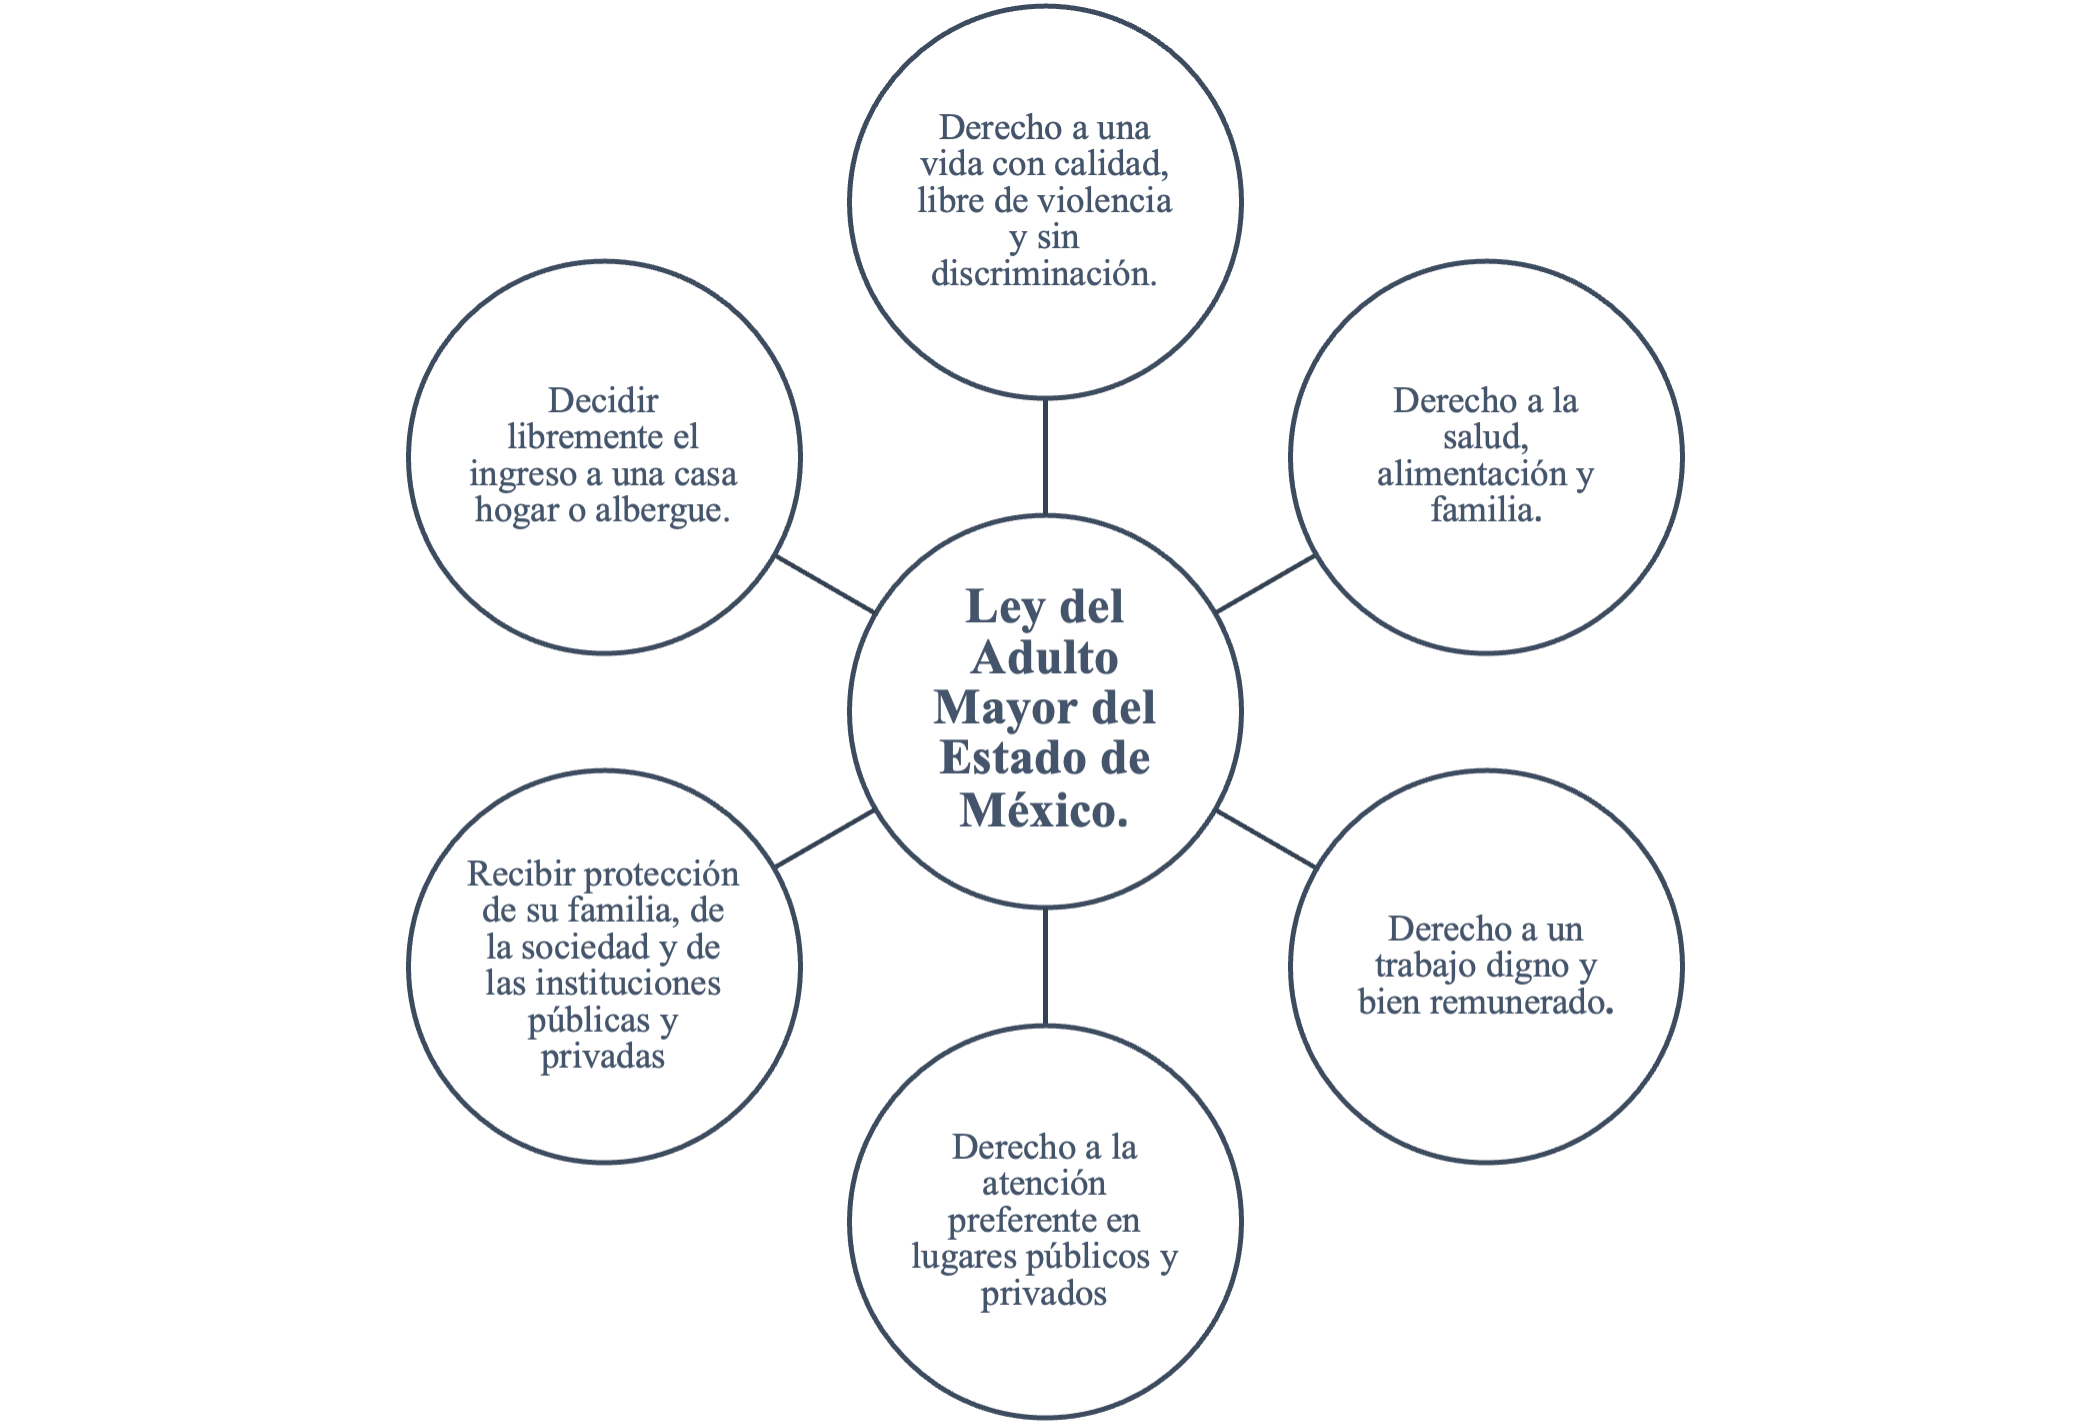
\includegraphics[keepaspectratio,alt={Elaboracióna partir del banco de datos de la página web del DIF Naucalpan}]{images/cap8libro2imagen1.png}}}

}

\caption{\label{fig-1}Elaboracióna partir del banco de datos de la
página web del DIF Naucalpan}

\end{figure}%

La Figura~\ref{fig-1} representa un conjunto de derechos fundamentales
para los adultos mayores establecidos en un marco legal que busca
garantizar su bienestar. Desde una mirada etnográfica refleja un marco
normativo bien intencionado, pero en la práctica, los adultos mayores
enfrentan múltiples barreras para acceder a estos derechos.

Un ejemplo de esta contradicción se presenta cuando los empleados
mencionan la dificultad de ofrecer apoyo a aquellos que carecen de
documentos oficiales, lo que se convierte en un obstáculo importante
para acceder a los servicios sociales. Le pregunte que pasaba si un
adulto mayor en situación de calle se acerca para solicitar apoyo me
dijo ``Sin papeles no podemos apoyarlos al sistema. Si quiere ayuda,
primero tiene tramitar su acta de nacimiento''. Este episodio evidencia
una contradicción estructural dentro del sistema de asistencia social:
existe presencia institucional y voluntad de brindar ayuda, pero al
mismo tiempo, los criterios administrativos como la exigencia de
documentos oficiales se convierten en barreras que excluyen a los más
vulnerables, como los adultos mayores en situación de calle. La
necesidad de cumplir con ciertos protocolos burocráticos como la
validación de documentos o el cumplimiento de requisitos específicos
para ser aceptado en los programas se convierte en una barrera para
aquellos que ya se encuentran en situaciones de extrema vulnerabilidad.
Esto crea una fractura entre lo que las instituciones prometen ofrecer y
lo que realmente pueden proporcionar, lo cual genera una paradoja: las
políticas y programas están diseñados para asistir a los más
vulnerables, pero se encuentran restringidos por un sistema rígido que,
en lugar de facilitar la ayuda, se convierte en un obstáculo.

Además, la estructura burocrática parece funcionar como un filtro, donde
los adultos mayores en situación de calle, muchas veces sin documentos,
son considerados casi ``invisibles'' ante las instituciones encargadas
de su atención. Esto nos lleva a una reflexión crítica sobre la
naturaleza de los servicios públicos y su capacidad para adaptarse a las
realidades cotidianas de las personas a las que supuestamente deben
servir. En muchos casos, las instituciones no logran conectar con las
necesidades urgentes y específicas de los individuos, ya que se limitan
a cumplir con un conjunto de requisitos formales sin comprender
completamente las circunstancias de cada caso.

\subsection*{Empatía y Limitaciones en la
Asistencia}\label{empatuxeda-y-limitaciones-en-la-asistencia}

En la oficina de Trabajo Social, logré hablar con una asistente social.
Me identifiqué como investigador, buscando entender cómo el DIF atendía
a adultos mayores en situación de calle. Entonces menciono ``estamos
limitados por las reglas para ello, solo canalizamos a un asilo''

Su respuesta resonó en mi mente. ``sin papeles, no existen''. La lógica
burocrática convierte a los adultos mayores sin hogar en sujetos
invisibles, ajenos a los derechos que, en teoría, deberían ser
universales. Los trabajadores del DIF, aunque expresan un fuerte deseo
de ayudar, reconocen que sus capacidades están rebasadas por la cantidad
de personas que requieren asistencia. La falta de recursos y espacios
disponibles es una constante en sus relatos. Estando en la oficina mire
el reloj y marcaba las 1:30 pm una hora que marca el umbral de la
oficina ya que los empleados están con el dilema de qué comerán en la
hora de la comida. Las fachadas de color gris con una arquitectura
funcional para brindar bienestar a la comunidad contrasta con el
concreto desnudo reflejando la frialdad institucional que había leído en
algunos otros textos antropológicos.

A pesar de la hora la persona responsable del área era muy amable y
prestaba atención a mis preguntas sentado frente a ella y cuaderno en
mano le pregunte \emph{¿Cree que las políticas actuales son suficientes
para atender a los adultos mayores que están calle?} Y en un tono amable
menciono ``contamos con un asilo, solo tiene la capacidad para atender a
20 personas, y no siempre hay recursos para recibir a quienes llegan''.
Esta afirmación reflejaba la profunda limitación de los recursos
disponibles, una limitación que no solo afecta la cantidad de personas
que pueden recibir ayuda, sino que también afecta la calidad de la
atención brindada. Esta falta de recursos se convierte en una fuente
constante de frustración tanto para los trabajadores como para las
personas que buscan ayuda, quienes se ven rechazadas o desplazadas en su
necesidad de asistencia.

Lo que se destaca a lo largo del trabajo de campo es la imposibilidad de
ofrecer un apoyo integral a los adultos mayores en situación de calle. A
pesar de los esfuerzos del personal, las intervenciones tienden a ser
reactivas y limitadas a medidas superficiales como proporcionar comida o
un espacio temporal. Sin embargo, no existen programas que aborden las
causas estructurales de la indigencia ni estrategias que permitan una
integración social más duradera. Los trabajadores institucionales,
aunque reconocen la importancia de su labor, también se sienten
atrapados en un sistema que, más allá de sus intenciones, no se ajusta a
las realidades concretas de las personas que intentan asistir.

El sentimiento de impotencia es una constante que aparece en los relatos
de los trabajadores. Muchos expresan su frustración al no poder ofrecer
soluciones definitivas a los problemas que enfrentan los adultos mayores
en situación de calle, quienes se ven atrapados en un círculo vicioso de
marginación y desprotección. Esta falta de respuestas efectivas, a pesar
de la empatía de los trabajadores, subraya las limitaciones inherentes
de un sistema que no ha sido diseñado para dar una respuesta adecuada a
esta población específica.

\subsection*{Exclusión Institucional y Percepción hacia los Adultos
Mayores}\label{exclusiuxf3n-institucional-y-percepciuxf3n-hacia-los-adultos-mayores}

El análisis de las percepciones de los trabajadores del INAPAM y el DIF
también reveló una clara exclusión institucional que afecta la atención
a los adultos mayores en situación de calle. Aunque el INAPAM se
presenta como una institución abierta a toda la comunidad, en la
práctica opera de manera restrictiva, dejando fuera a aquellos que no
cuentan con una vivienda estable ni documentos que avalen su derecho a
recibir asistencia. Esta exclusión social se refleja en la vida
cotidiana de los adultos mayores que viven en las calles de Naucalpan. A
pesar de que existen espacios institucionales como el DIF 5 de mayo, DIF
Arcos, Casa de día ``Sonreír a la vida'' o el INAPAM, la realidad es que
las condiciones de acceso a estos lugares son limitadas por las
burocracias internas y los protocolos administrativos. La falta de
adaptabilidad de estos servicios para responder a las necesidades de los
adultos mayores que no pueden cumplir con los requisitos establecidos
(como la falta de documentos oficiales o la falta de un domicilio)
expone la fragilidad del sistema de bienestar social.

Un testimonio clave de una trabajadora del DIF muestra esta tensión: ``A
los adultos mayores los vemos como personas que cargan con mucho peso de
la sociedad, son abandonados por sus familias y, aunque nos gustaría
hacer más por ellos, no tenemos los recursos para brindarles el apoyo
que necesitan.'' Esta reflexión resalta el contraste entre las buenas
intenciones de los trabajadores y las limitaciones estructurales que
enfrentan dentro de un sistema incapaz de ofrecer respuestas efectivas.
Además, la etnografía muestra otro desafío: la resistencia de algunos
adultos mayores a recibir asistencia. Ya sea por desconfianza hacia las
instituciones o por el deseo de mantener su autonomía, muchos prefieren
rechazar la ayuda, incluso en condiciones de extrema marginalidad. Esta
compleja relación entre las instituciones y los adultos mayores refleja
una doble exclusión material, al no acceder a recursos básicos, y
simbólica, al quedar fuera del sistema de protección social.

Algunos de los adultos mayores entrevistados relatan que las visitas a
estas instituciones suelen ser breves e ineficaces, ya que no se le
ofrece una solución sostenible a su situación\footnote{Adultos mayores
  de Naucalpan: percepciones sobre el estado, la familia y la sociedad
  desde la indigencia (2024)}. En muchos casos, la ayuda se limita a una
intervención temporal como entregar comida o permitirles descansar por
un breve periodo de tiempo, pero no se desarrollan programas de
acompañamiento integral que garanticen una mejora duradera en su calidad
de vida. A través de esta etnografía, se hace evidente que la atención
institucional es insuficiente para abordar las complejas necesidades de
los adultos mayores en situación de calle, lo que refuerza la percepción
de que, a pesar de las intenciones, el sistema está fallando en
proporcionar una solución adecuada.

La etnografía realizada revela una profunda brecha entre el discurso
institucional y las practicas cotidianas en la atención y prevención a
los adultos mayores en situación de calle. El DIF y el INAPAM, proyectan
narrativas de protección y dignificación, pero en la práctica, la ayuda
que ofrecen es limitada, burocratizada y, en muchos casos, ineficiente.
Los testimonios recopilados durante el trabajo de campo evidenciaron
estas afirmaciones. Algunos adultos mayores han expresado que no conocen
el apoyo que estas instituciones pueden brindar. La asistencia social se
reduce a la entrega de alguna cobija, la posibilidad de descansar
algunas horas en un albergue, pero no se les ofrece un acompañamiento
integral que aborde las causas estructurales de su situación.

Lo mencionado por una trabajadora del DIF destaca esta tensión: ``a los
adultos mayores los vemos como personas que necesitan mucho apoyo, no
tienen a nadie, nos gustaría apoyar, pero no tenemos los recursos''.
Esta declaración es una constante entre los miembros de estos
organismos. Además, el trabajo de campo muestra que la relación entre
estas instituciones y los adultos mayores en situación de calle es
compleja. Algunos no saben del apoyo que podrían recibir y otros la
rechazan debido a la desconfianza hacia todas las personas que los
rodean. Esta actitud refuerza el círculo de exclusión, donde los adultos
mayores no solo enfrentan barreras materiales, sino también simbólicas,
quedando ``invisibles'' ante el aparato burocrático. Esta visita al DIF
dejó al descubierto más que procedimientos burocráticos ineficientes.
Fue un retrato de cómo las instituciones replican violencias
estructurales al no adaptar sus programas a realidades complejas. Los
adultos mayores en situación de calle no solo enfrentan la pérdida de un
hogar o redes familiares, sino también la negación simbólica de su
derecho a existir dentro del sistema.

La estructura administrativa funciona como un filtro que excluye a
quienes no cumplen con ciertos requisitos, como la posesión de
documentos oficiales, reforzando lo que Pierre \textcite{Bourdieu1994}
denomina ``violencia simbólica'' el autor describe que hay formas de
dominación que operan de manera sutil legitimadas por el Estado. En el
contexto de la asistencia institucional a adultos mayores en situación
de calle en Naucalpan, la violencia simbólica se evidencia en prácticas
que, bajo el discurso del cuidado y la protección, reproducen estigmas y
jerarquías sociales. Así, las instituciones terminan perpetuando la
marginalidad que intentan combatir, incapaces de adaptarse a las
realidades cotidianas y urgentes de esta población vulnerable.

\section*{Entre la institución y la realidad: reflexiones
inconclusas}\label{entre-la-instituciuxf3n-y-la-realidad-reflexiones-inconclusas}

\markright{Entre la institución y la realidad: reflexiones inconclusas}

La investigación realizada en Naucalpan, Estado de México ha permitido
evidenciar que la asistencia institucional a los adultos mayores en
situación de calle enfrenta limitaciones estructurales y operativas.
Aunque los programas sociales están diseñados para garantizar el
bienestar de este sector, en la práctica, las barreras burocráticas, la
falta de recursos y rigidez de los protocolos impiden una atención
efectiva y digna. La vejez y la situación de calle es un fenómeno que
pone en tensión el discurso oficial de las instituciones ya que las
realidades cotidianas de exclusión y marginalización se hace presentes.

A través del trabajo de campo, se ha observado que la burocracia
institucional opera como un mecanismo de filtrado que deja de fuera a
quienes no cumplen con los criterios administrativos, reproduciendo una
violencia simbólica que los condena a convertirse en sujetos
invisibilizados. Si bien algunos trabajadores sociales muestran empatía,
las restricciones de un sistema los limita en su capacidad de acción,
consolidando un modelo de asistencia asistencialista que perpetua la
dependencia de vivir en las calles y depender de la solidaridad de la
sociedad. En ese sentido, esta investigación ha permitido problematizar
la relación entre el Estado y la vejez en situación de calle, destacando
la necesidad de repensar los programas de asistencia desde un enfoque de
derechos. Los datos recopilados durante el trabajo de campo sugiere que
las políticas públicas deben de dejar de lado la idea de ser
asistencialista y optar estrategias integrales que atiendan no solo las
necesidades de cubrir una agenda pública y material, sino también los
problemas estructurales que perpetúan la vida en la calle de los adultos
mayores.

Por lo tanto, en este trabajo se opta por dejar abiertas algunas líneas
de reflexión mediante preguntas puntuales sobre el futuro de la
asistencia social. ¿Es posible que los programas sociales garanticen una
vejez digna a quienes, en su juventud, no lograron consolidar una vida
laboral estable? Esta interrogante surge a partir de la premisa de que
muchos adultos mayores en situación de calle enfrentan esta realidad
debido a la falta de éxito y estabilidad en los ámbitos laboral, social
y familiar a lo largo de su vida. ¿Cómo se puede apoyar a las personas
sin identidad burocrática? Abordar este problema administrativo es
fundamental, ya que muchas personas en situación de calle quedan
excluidas de los programas sociales debido a la falta de documentos que
acrediten su identidad. Esta ausencia no solo las margina del acceso a
derechos básicos, sino que también las invisibiliza dentro del sistema.
Por lo tanto, es crucial desarrollar políticas más inclusivas y
eficientes que realmente transformen la vida social de estas personas,
en lugar de limitarse a cumplir con un mecanismo institucional que solo
simula brindar ayuda.

\printbibliography[heading=subbibliography, title={Referencias Bibliográficas}]

\bookmarksetup{startatroot}

\chapter{Cruce de activismos, cruce de motivaciones: etnografías desde
dos instituciones de
cuidado}\label{cruce-de-activismos-cruce-de-motivaciones-etnografuxedas-desde-dos-instituciones-de-cuidado}

\addtocontents{toc}{\protect\hspace{1.5em} Laura Isabel Matamala Lienlaf \par}
\markboth{Etnografías, activismos, motivaciones y cuidados}{}
\begin{flushright}
\Large Laura Isabel Matamala Lienlaf \footnote{Maestra en Antropología Social por la Universidad Iberoamericana Ciudad de México y licenciada en Ciencias Religiosas por la Universidad Pontificia de México. Sus investigaciones se centran en el estudio de las violencias, la desaparición forzada de personas, las prácticas de memoria y los procesos de búsqueda impulsados por familiares de personas desaparecidas, particularmente en colaboración con colectivos de búsqueda en México. También ha desarrollado trabajos sobre teología y violencias desde una perspectiva interdisciplinaria. Contacto: \href{lauraisabelmatamala@gmail.com}{lauraisabelmatamala@gmail.com}}
\end{flushright}

\section*{Introducción}\label{introducciuxf3n-6}

\markright{Introducción}

En el trabajo humanitario ---principalmente aquel de inspiración
cristiana--- las fronteras entre lo religioso, lo político y lo ético se
entrelazan en el día a día. Este artículo sostiene que las instituciones
de cuidado con fundamentos religiosos no pueden entenderse únicamente
como espacios de caridad despolitizada, sino como escenarios donde se
ensamblan diversas formas de activismo --humanitario, político y de
derechos humanos-- a través de prácticas guiadas por la fe. A partir de
una experiencia de vida y trabajo como religiosa en dos instituciones
mexicanas, se analiza cómo se articulan motivaciones, resistencias y
formas de agencia en contextos marcados por el cuidado y la desigualdad
estructural.

Las revisitas etnográficas tienen un potencial analítico particularmente
provechoso para desentrañar estructuras, actores, acciones y motivos de
quienes llevan adelante labores humanitarias en instituciones de
cuidado. El paso del tiempo permite decantar la experiencia y retornar
hacia ella en un ejercicio de sistematización, que revela y sintetiza la
porosidad de ser investigadora y activista al mismo tiempo.

Particularmente me remito a dos experiencias de servicios humanitarios
que desarrollé en la Ciudad de México y Lázaro Cárdenas, Michoacán,
mientras era miembro de una congregación religiosa de espiritualidad
carmelitana. El primero de ellos, un albergue coordinado por una
Institución de Asistencia Privada (IAP) de voluntarias inspiradas por un
santo francés, dedicado a la atención de enfermos que acuden a la zona
de hospitales en el sur de la CDMX para tratamientos médicos; el
segundo, una casa hogar (AC), sostenida por una empresaria nacional,
destinada al cuidado, educación y promoción de niños y niñas de las
familias más pobres de la región. En estos escenarios, el papel del
humanitarismo se presenta como el núcleo de la vocación de servicio,
pero, a diferencia de lo que el discurso religioso suele afirmar, este
está íntimamente imbricado con el activismo y sus diferentes
categorizaciones.

Si bien estos dos lugares están claramente definidos como instituciones
de inspiración cristiana de asistencia a los necesitados y sin fines de
lucro, están atravesados por una serie de políticas que permiten
donaciones privadas no siempre esclarecidas, y una distribución de estas
de modo desigual. Entonces, ¿qué son en la práctica estas instituciones?
La respuesta depende del lugar desde el que se las mire. Desde la
perspectiva del patronato o empresariado: una obra de caridad que ayuda
a los necesitados y, al mismo tiempo, beneficia sus intereses; desde las
religiosas: una misión que responde a su deseo de servir al mundo porque
Cristo se lo pide; desde los beneficiarios: un lugar de salvación que
les tendió la mano cuando más lo necesitaban. En estas instituciones de
cuidado se mezclan distintas motivaciones de lo humanitario. Por esta
razón, nos detendremos especialmente en las `razones humanitarias' de
las religiosas presentes en estos albergues que no se puede clasificar
como `puramente' religiosas en virtud de una consagración, sino que se
entrelazan con los tres tipos de activismos propuestos por
\textcite{PodgornikJakil2021}: humanitario, de derechos humanos y
político. Entonces ¿ante qué tipo de activismo nos encontramos? Nuestra
hipótesis propone que es un ensamblaje de los tres. Por ello, la
pregunta se reformula: ¿cómo se intersectan, en la práctica, los
distintos tipos de activismos propuestos por Podgornik-Jakil y Bens en
dos instituciones de cuidado?

En un momento segundo y no menos importante, abordaremos estos dos
espacios de labor humanitaria como un sitio donde convergen y trabajan
para un mismo fin diversos tipos de actores que, desde las funciones
peculiares que desempeñan, posicionan a los receptores de ayuda en un
lugar aparentemente estático. Sin embargo, el acercamiento etnográfico
permite vislumbrar los distintos tipos de resistencia y agencia que
desarrollan, aun en medio de una estructura que pareciera totalmente
constreñida. Por eso también buscamos identificar y diferenciar la
escala de intermediadores que tiene el albergue de enfermos y la casa
hogar, donde los miembros de cada escalón negocian márgenes de acción y
acceso en beneficio de quienes se albergan allí. Así, respondemos a la
pregunta: ¿qué tipo de agencia y resistencias encontramos en la escala
de intermediarios?

Todas estas preguntas las intentaremos responder desde mi propia
experiencia en estos lugares en los que viví a tiempo completo entre el
2016 y 2021. Claro está, complejizando principalmente desde los
postulados de la `antropología comparada' de
\textcite{PodgornikJakil2021}, la `razón humanitaria' de
\textcite{Fassin2016}, la `utilidad situada' de
\textcite{Yotebieng2020}, la `antropología del humanitarismo' de
\textcite{Redfield2011} , la `necesidad de ayudar' de
\textcite{Malkki2015} y otras literaturas complementarias que nos
servirán para abordar la complejidad de las instituciones de cuidado y
examinar el papel ---confuso--- del activismo humanitario-religioso en
dicha labor.

Para ello, recurro a una metodología autoetnográfica, entendida como un
enfoque cualitativo que permite explorar, desde la experiencia personal,
procesos culturales más amplios. La autoetnografía, como plantean
\textcite[17-18]{Ellis2010}, es simultáneamente un proceso y un
producto: el investigador articula principios de autobiografía y
etnografía para describir y analizar su vivencia con el fin de
comprender fenómenos sociales y culturales. Es también un acto político
y ético, pues reconoce que la investigación se sitúa en la intersección
entre lo personal, lo estructural y lo relacional.

Este enfoque fue especialmente pertinente para el presente artículo, ya
que durante más de cinco años viví como religiosa en ambas
instituciones, desempeñando entre otras cosas, el rol de cronista dentro
de la comunidad, una función establecida en la organización de la vida
cotidiana de las congregaciones femeninas. Esta tarea implicaba llevar
un registro escrito diario de las actividades, tensiones y momentos
significativos de la vida común. Con el tiempo, esas notas, sumadas a mi
memoria corporal y afectiva, se transformaron en un archivo interno
desde el cual revisité la experiencia, ahora desde una mirada
antropológica. La aplicación de esta metodología fue doble: implicó
tanto la revisión de los registros y vivencias pasadas como una
relectura crítica de mi implicación en las dinámicas institucionales.

Considero que la autoetnografía fue el método más adecuado para esta
investigación, ya que me permitió acceder ---como sujeto plenamente
implicado--- a un campo en gran medida hermético para quienes no forman
parte del mundo religioso. La posibilidad de narrar y analizar desde
dentro no solo ofrece una perspectiva privilegiada sobre las
motivaciones, tensiones y formas de agencia que configuran el activismo
en contexto de cuidado, sino que también revela la complejidad de esas
prácticas cuando se examinan desde la frontera difusa entre lo religioso
y lo político.

Si bien en este artículo me concentro principalmente en el papel de las
religiosas y, en menor medida, de los voluntarios, esta delimitación
responde tanto a mi lugar de enunciación como a la metodología empleada.
La autoetnografía me permite acceder de manera directa y \emph{emic} a
la experiencia cotidiana de quienes compartieron la vida comunitaria
conmigo. En contraste, otros actores relevantes del ecosistema
institucional ---como trabajadores sociales, médicos, personal
administrativo o donantes--- participaron de forma más periférica, y no
fue posible acceder con profundidad a sus motivaciones, decisiones o
vivencias desde el lugar que ocupé. Por esta razón, el presente trabajo
se centra en aquellas figuras con las que existió un vínculo más
profundo en la cotidianeidad, sin que ello implique desconocer la
complejidad del entramado institucional en su conjunto.

\section*{Primeras discusiones}\label{primeras-discusiones}

\markright{Primeras discusiones}

Para los fines de este artículo, presentaremos una revisión literaria en
concordancia a cómo queremos desengranar el argumento central de la
exposición: la superposición de los distintos tipos de activismos y las
formas de resistencia que emplean los actores en una institución
humanitaria, desde una revisita etnográfica en primera persona. Por lo
tanto, los postulados teóricos no obedecerán a un orden cronológico,
sino a una razón argumentativa.

Encabezando los antecedentes, la obra del antropólogo alemán Ziga
Podgornik-Jakil es una referencia obligada para los estudios de
activismo político desde una etnografía de movimientos sociales
vinculados a temas de asilo y trabajo. Particularmente su artículo,
`Hacia una antropología comparada del activismo: formaciones de
identidad activista en Alemania y Uganda' \autocite{PodgornikJakil2021}
es el marco fundamental con el que dialoga este texto.

En dicha obra se encara la discusión actual sobre el activismo
humanitario, el activismo por los derechos humanos, y el activismo
político que operan en el discurso público o formal de los activistas,
pero que, en lo concreto, no se encuentran como formas puras y aisladas.
Antes bien, son categorías que traspasan sus propias delimitaciones y,
en donde, cada una de ellas atribuye una `posición-sujeto' a las
personas destinatarias de la ayuda. A lo largo de sus páginas, insta a
desacreditar las posiciones correctas del sujeto, para prestar atención
a condiciones materiales y diversos tipos de agencia que desarrollan los
actores, aun en condiciones desfavorecidas.

Sus postulados nos son útiles para hacer legible las dos instituciones
de cuidado que presento. Particularmente su clasificación de: 1)
Activismo humanitario ocupado en atender el sufrimiento de la humanidad;
2) Activismo por los derechos humanos que lucha por el cumplimiento y
defensa de derechos universales; 3) Activismo político que promueve
sujetos autónomos e impulsa agendas políticas
\autocite[300]{PodgornikJakil2021}, nos ayudan a entender el tipo de
socorro que se les brinda a las poblaciones carenciadas, y la
`posición-sujeto' ---imaginada--- que se les asigna.

Estas categorías permiten comprender cómo, en las instituciones
estudiadas, los actos de cuidado no se inscriben exclusivamente en una
lógica religiosa o humanitaria, sino que se articulan también como
formas de resistencia política, defensa de derechos y posicionamientos
éticos situados. A lo largo del texto se analizará cómo estos tipos de
activismo aparecen ensamblados ---y, a veces, en tensión--- en la
práctica cotidiana del albergue y la casa hogar.

Del primer tipo de activismo, deviene la posición de víctima sufriente,
reducida a un receptor pasivo de ayuda, que, por tanto, debe responder
con gratitud y obediencia. Desde la experiencia del albergue, esto se
traduce como en el ideal de un albergado bueno, disponible para ayudar
en las labores de limpieza y cumplidor de los ritos católicos; y desde
la casa hogar, en niños bien portados, inteligentes y que se saben todas
las oraciones.

En la segunda categoría, se les ubica como sujetos de derechos y
libertades individuales. Concretamente en el albergue, acompañando y
empoderando para que no se dejen pasar a llevar por médicos y personal
administrativo de los hospitales; y en la casa hogar, para que las
madres de los niños exijan un salario justo en sus trabajos; mientras
que el tercero ven a sus beneficiarios como actores políticos autónomos
y pares en una lucha política común \autocite[301]{PodgornikJakil2021};
siendo ellos capaces de llevar adelante demandas y organización de
sindicatos para pelear lo justo, tanto en el albergue como en la casa
hogar.

De esta manera, la `posición de sujeto' y el ordenamiento de los
activismos, son dos conceptos que nos permiten profundizar en la
relación que tienen entre sí dichos activismos, desde una vía empírica
que examina sus reflejos en estos dos establecimientos humanitarios.

Sumado a esto, otro bloque fundamental de Podgornik-Jakil y Bens es la
formación identitaria de los actores de estos activismos. Para
visibilizar este proceso, presentan dos estudios de caso. El primero
aborda la atención a refugiados en Berlín durante 2015 y 2016.
Inicialmente, el enfoque fue humanitario, cubriendo sus necesidades
inmediatas; sin embargo, pronto evolucionó hacia la exigencia de
derechos, con el respaldo de clínicas jurídicas, y finalmente derivó en
un activismo político que buscaba un cambio social más profundo,
trascendiendo el marco legal.

El segundo caso, aborda la justicia transicional en el norte de Uganda
en el que, producto de un conflicto armado el 90\% de la población fue
desplazada y obligada a vivir en campamentos precarizados, donde la
mayor parte del tiempo imperó un modelo humanitarista colonialista,
dejando en la población la sensación de humillación: ``¿Te imaginas la
indignidad que conlleva verse obligado a comer alimentos proporcionados
por la comunidad internacional todos los días durante años? ¿No poder
trabajar, cultivar para mantener a la propia familia?''
\autocite[307]{PodgornikJakil2021}. Esta situación empujó a los
activistas de derechos humanos a que se entendiera la política como un
tema que involucra todos los aspectos de la vida y, los activistas
políticos, se preocuparon especialmente por llevar adelante iniciativas
por la paz que, no necesariamente implicó procesos de justicia y
reparación.

Estos dos registros etnográficos servirán de espejo para abordar
situaciones similares tanto en el Albergue como la casa hogar: ambos
recintos reciben donaciones de alimentos (no pocas veces en mal estado)
por parte de grandes cadenas de supermercados, donde en muchas ocasiones
tanto albergados como niños tenían que repetir la misma comida por
varios días. En algunas jornadas, era tal la descomposición de la comida
(ya preparada) que se recibía (también los hospitales donan las comidas
que se les quedan) que se tenía que tirar. Ante esto las religiosas nos
ocupábamos de presentar reclamos oficiales a las instancias necesarias,
ya que era inaudito que estuvieran donando comida estropeada a enfermos
y niños vulnerables. A pesar de los esfuerzos en la casa hogar para
prevenir la violencia intrafamiliar, como talleres y apoyo legal, los
intentos de intervención llegaban demasiado tarde. Esto se evidenció
cuando un padre asesinó a una de las mujeres beneficiarias durante una
jornada de clases.

En este sentido, los casos del albergue y la casa hogar muestran
trayectorias similares: acciones inicialmente inscritas en una lógica
humanitaria o asistencial se complejizan al incorporar dimensiones de
denuncia, acompañamiento legal y organización comunitaria. Como los
ejemplos de Berlín y Uganda, lo político y lo humanitario no son esferas
separadas, sino procesos que se entretejen en la experiencia cotidiana
de los actores.

Esta antropología del activismo de Podgornik-Jakil y Bens, se entrecruza
con la problematización de la antropóloga Benedetta Rossi con respecto a
la relación entre receptores y donantes. Especializada en la historia
laboral africana, esclavitud, migración y ayuda al desarrollo
planificado, se cuestiona por la separación epistemológica y social que
se hace de ambos grupos sociales como si pertenecieran a `mundos de
vida' separados. En su capítulo de libro titulado `Políticas de ayuda y
estrategias de beneficiarios en Níger' \autocite{Rossi2006}, aborda de
manera indirecta, el postulado principal de Podgornik-Jakil y Bens: los
campesinos de Níger son convertidos en simples beneficiarios de
proyectos para paliar la desertificación de su territorio. Una clara
asignación de una posición de sujeto imaginada.

Este posicionamiento como receptores de beneficio se construye mediante
un proceso que Rossi lo llama `noción de sensibilización', es decir, una
serie de prácticas que están pensadas y destinadas a que los habitantes
del África Occidental acepten los cambios propuestos sin inhibir la
expresión de sus ideas y la capacidad de cuestionar los problemas que el
mismo proyecto vaya suscitando. Así, quienes completan dicho proceso,
terminan reproduciendo formas y racionalidades propias del desarrollo.

Añadido a esto, está el empeño por parte del desarrollador para que el
campesino tome conciencia de que necesita cambiar su estilo de vida, sus
modos de producción, su organización social y hacerse más responsable en
el marco de la lucha contra la desertificación \autocite[36]{Rossi2006}.
Se obliga así a forjar y representar un tipo de identidad que atribuye
categorías morales y responsabilidades particulares solo a ciertos
actores; son los impulsores del desarrollo los que deciden quiénes deben
modificar su vida, donde la clave de solución es el cambio de mentalidad
por medio del proceso de sensibilización.

A simple vista, pareciera un transcurso mecánico de conversión de
sujetos a meros reproductores de una operación desarrollista pero, lo
que advierte Rossi es un punto medio: a pesar de ser reducidos a
beneficiarios, los receptores no pierden su agencia, sino que la nueva
posición les permite mejorar sus condiciones y ser conscientes de las
nuevas oportunidades que tienen en puertas; en sus ``formas de utilizar
el proyecto presuponen una conciencia realista de lo que pueden lograr
en virtud de su condición de receptor'' \autocite[29]{Rossi2006}.

Este vértice nos servirá para abordar la agencia que tienen los enfermos
y acompañantes del Albergue que, posicionados desde su papel como
receptores de ayuda, se mueven de manera estratégica para lidiar tanto
con el personal administrativo como con las hermanas, y así maximizar
los beneficios a los que pueden acceder. En palabras de Rossi, son
conscientes de las oportunidades que tienen como receptores. Consciencia
que es compartida también por los trabajadores y las hermanas que, desde
sus propios estatus maniobran según propia deliberación, las situaciones
de los albergados y sus necesidades. Es decir, pueden adoptar posturas
contradictorias como: apropiarse de algunas donaciones materiales,
decidir por simpatía a qué enfermos darles las ayudas, a qué
acompañantes liberar del servicio de limpieza a cambio de favores; pero,
al mismo tiempo, pueden ir más allá de las reglas y discursos, logrando
que los albergados más pobres reciban lo necesario y hacer mucho más de
lo que está estipulado en sus contratos. Un enclave que no deja de ser
contradictorio, pues desde su ubicación como donantes son también
conscientes de las oportunidades que tienen al ocupar tal puesto. Así,
tanto receptores como donantes no operan desde lógicas diferentes ni
configuran mundos de vidas separados, sino que ambos desarrollan
estrategias diferenciadas según el contexto desde donde se ejerzan. En
la práctica, aquí la separación entre `otorgantes y receptores de ayuda'
no es para nada útil.

Lo específico de las tácticas de los beneficiarios pasa por un ojal
obligado: contar y profundizar en sus historias todas las veces que sea
posible. A este aspecto narrativo de la ayuda se dedica Kelly A.
Yotebieng en su capítulo de libro titulado `Estamos cansados de contar
nuestras historias'. En dicho texto, expone su proceso de conversión al
activismo que, inició con preguntas vitales luego de cada trabajo de
campo: ``las personas no me comparten sus historias íntimas solo para
ayudarme a terminar mi tesis {[}\ldots{]} historias de violencias,
asesinatos, desplazamientos'' \autocite[151]{Yotebieng2020}; todo un
repertorio de tragedias que esperaba un compromiso de su parte.

Un aspecto central de su acercamiento a campo fue dejar en claro sus
intenciones y a qué organizaciones no pertenecía. Con frecuencia la
veían como enviada de la ACNUR y, por tanto, pensaban que, si les
contaban sus historias, le podría ayudar a mejorar su situación; las
expectativas eran altas. No pocas veces, registró quejas como:
``¿Cuántas veces necesito contar mi historia a un extraño mientras lloro
para ser considerado digno de ser un refugiado?''\footnote{Traducción
  del inglés propia.} \autocite[155]{Yotebieng2020}, es decir, tienen
que despejar toda duda para poder acceder a los beneficios
correspondientes y en todo momento demostrar la valía de su estatus.
Testimonio muy similar a casos del Albergue donde los enfermos me
decían: ``¿qué tan trágica tiene que ser mi enfermedad para que me
ayuden?'' , o en la casa hogar: ``¿qué tan pobre tengo que ser para que
mi hija ingrese? Si tengo un refrigerador ¿ya no entro?''.

Una utilización del dolor de las personas en instituciones humanitarias
que es un paso forzoso para poder acceder a los legítimos derechos de la
condición de refugiados, por ejemplo. En este ejercicio constante de
narrar sus historias, Yotebieng se percata que los participantes de su
investigación se comienzan a etiquetar a sí mismos según la
categorización que las ONG les asignaba: persona mayor, niño vulnerable,
enfermo crónico. Así, el hecho de contar y volver a contar sus historias
era una forma de capital para acceder a los servicios, ser catalogados
en un grupo prioritario, para forjar identidades indivisibles de esas
etiquetas \autocite[157]{Yotebieng2020}. Este punto será muy importante
en el análisis posterior, donde profundizaremos en los procesos de
ingreso del albergue y casa hogar, los filtros sociales que se aplican
como: estar en extrema pobreza, sin contar con el apoyo de terceros,
tener una enfermedad grave y poder contar con un acompañante para
hospedarse.

Finalmente, el último bloque de autores estará dedicado a problematizar
las intenciones de los actores humanitarios, con especial atención a la
evidencia empírica que presentaré sustentada en mis 10 años de
religiosa.

Para este cometido, Didier Fassin será central para discutir las
`razones humanitarias' de quienes se dedican a dicho servicio. En su
libro La razón humanitaria nos sitúa en la reconfiguración política de
cómo se gestionan las vidas precarias, atravesado por un profundo
despliegue de sentimientos morales en las prácticas de asistencia. Por
tal razón, se propone escrutar los efectos que tienen las acciones de
los gobiernos humanitarios en el tratamiento de las poblaciones
excluidas, enarbolando una escala de valores que tiene a lo `moral' como
objeto de estudio. Afirma Fassin que los sentimientos morales son el
corazón de las políticas actuales, sustentando discursos y legitimando
prácticas. El destinatario principal de estas políticas son los
desposeídos. Pero dichas emociones están atravesadas por una forma mucho
más acabada: la política de la compasión afincada en la doctrina
cristiana, pero que al mismo tiempo va mucho más allá de ella misma.

Algunos conceptos centrales del análisis de Fassin nos servirán para
profundizar en la interpretación de estas instituciones de cuidado.
Términos como 1) `gobierno humanitario' comprendido como el despliegue
de sentimientos morales en políticas contemporáneas; 2) `humanitario'
como noción global de humanidad de la que se desprenden derechos y, como
de igual condición desde donde surge la obligación de asistencia al
otro; 3) `sentimientos morales' que surgen cuando volteamos a mirar a
los más pobres y desafortunados y los convertimos en objetos de atención
humanitaria, pero, a la espera de que el receptor sea agradecido y no se
posicione como sujeto que demanda derechos; 4) `compasión' como
ejercicio de arriba hacia abajo, desde los ricos a los pobres. Todas
estas nociones se pondrán en diálogo con las experiencias etnográficas
caracterizadas por formas de gobierno internas: en el albergue, la
escala es la siguiente: 1) patronato de voluntarias (son quienes
financian); 2) comunidad de hermanas (religiosas que sostienen la obra);
3) albergados (incluye a los enfermos y sus acompañantes); cada uno con
su serie propia de valores, pero teniendo en el centro siempre al
destinatario principal: el enfermo. En cuanto a la casa hogar, el
escalafón es el siguiente: 1) Empresaria benefactora; 2) comunidad de
religiosas; 3) niños y familias pobres. Tienen en común la forma de
organización, con un intermediario siempre ubicado en la mitad: las
hermanas que median entre el patronato y los beneficiados son el corazón
de la institución. En ambos contextos se da un tipo de administración
humanitaria muy coincidente con otras ONG, donde los más desfavorecidos,
según el contexto donde se encuentre, son siempre los más carenciados;
lo específico de estas dos instituciones es el sentimiento de compasión,
inspirado principalmente en la tradición cristiana.

Además, Fassin también nos ayudará a analizar tanto el albergue y la
casa hogar como dos instituciones humanitarias que están habitadas por
contradicciones, enriquecidas por una etnografía que nos permitirá
acercarnos a las lógicas de los actores y cómo se justifican las
acciones \autocite[25]{Fassin2016}; entrando al escondite de los
detalles, accediendo a certeza y dudas, claridad y oscuridad, prejuicios
y reflexividad; un espacio habitado por tensiones
\autocite[28]{Fassin2016}.

Para completar el aterrizaje en la compasión, Peter Redfield y Erica
Bornstein \autocite*{Redfield2011} nos adentran en la pregunta ¿por qué
el cuidado a extraños tiene un papel tan protagónico? Para responder al
cuestionamiento, emprenden una revisión de la historia del sufrimiento y
la caridad, junto con los esfuerzos humanitarios para socorrer a quien
lo necesita. En su texto `Fuerzas de la compasión', afirman al igual que
Fassin, que en el centro del discurso moral internacional se encuentra
el impulso humanitario para aliviar el sufrimiento; siendo utilizado
como un recurso propiamente estatal.

Para acceder a una capa más profunda presentan una genealogía del
`humanitarismo' y la especificidad que lo diferencia y relaciona con
`hacer el bien' al mundo. Tradiciones religiosas de ayuda y caridad,
entrarán en la disputa sobre qué define el valor de la humanidad y cómo
la opción creyente motiva la empatía humana. Defensores de
humanitarismos y entidades religiosas se acercan en su interés por
mejorar la condición humana y se alejan en cuanto que los primeros
procuran satisfacer todas las necesidades materiales y temporales,
mientras que la segunda, se esmera por cuidar y cultivar también la
dimensión espiritual de los beneficiarios.

En esta última vertiente, Redfield y Bornstein, se enfocan en las
respuestas religiosas ante el sufrimiento humano bajo las formas de
caridad, ministración y cuidado por parte del budismo, islam, judaísmo y
cristianismo. Por razones de este ensayo, nos detendremos en la religión
cristiana y su máxima de fe: vestir al desnudo, dar de comer al
hambriento, dar de beber al sediento, recibir al forastero, cuidar al
enfermo, visitar al encarcelado; todas entendidas como obras de
misericordia que se le hacen al mismo Jesús, a través de los pobres. De
esa manera, nos introduciremos a las motivaciones de las religiosas como
intermediarias entre los bienhechores y la población asistida, donde
finalmente se entrecruzan impulsos humanitarios, activistas, religiosos
y de demanda moral. No podríamos hablar de una forma intacta de
motivación.

\section*{Presentación etnográfica del Albergue y Casa
Hogar}\label{presentaciuxf3n-etnogruxe1fica-del-albergue-y-casa-hogar}

\markright{Presentación etnográfica del Albergue y Casa Hogar}

Desde los inicios del albergue su misión y visión se concentró en
brindar hospedaje, alimentación, apoyo en tratamientos y medicamentos a
enfermos, venidos de otras partes de la República y que, no tienen la
posibilidad de pagar una pensión mientras reciben sus tratamientos en
los hospitales de especialidad. Las hermanas carmelitas llegaron años
después, a solicitud de las voluntarias, para ofrecer asistencia
espiritual a los enfermos y actuar como personal de confianza, viviendo
en las instalaciones las 24 horas para encargarse de todo.

El panorama general que describo a continuación y los casos puntuales
que utilizaré en el análisis, son de primera mano y recogidos mientras
viví en el albergue entre los años de 2018 y 2021, siendo religiosa de
dicha congregación.

El Albergue tiene una capacidad para recibir a 143 personas. Los
requisitos fundamentales para ser admitidos son: estar enfermos y tener
citas en algunos de los hospitales de la zona, contar con un
acompañante, ser foráneos, no tener los recursos suficientes para
alimentación y hospedaje, apartar su lugar con una semana de
anticipación y poder cubrir la cuota de recuperación diaria de \$15. Ese
dinero les da derecho a una cama y las cobijas necesarias que se
renuevan cada tres días, tres comidas calientes al día, agua caliente,
lavandería, acompañamiento psicológico, social y espiritual, acceso a
ayudas para costear tratamientos, medicamentos y servicios funerarios.

En el tema de distribuciones, se les asigna las habitaciones
correspondientes según con quien venga acompañado el enfermo: si viene
mujer con mujer, se les envía a las habitaciones comunes de mujeres, lo
mismo sucede con los varones. En cambio, si son pareja, hay espacios
propios para ellos. Cuando el enfermo es un bebé o menor de edad, se le
envía al área de niños que tiene todo lo necesario para que una familia
pueda hospedarse allí, también en caso cuando el enfermo está muy grave,
tiene una enfermedad contagiosa o cualquier otra agravante que le impida
estar en los cuartos comunes, puede solicitar una de las 5 habitaciones
privadas. Es importante mencionar que hay albergados que pueden estar
desde 2 días, 3 semanas, 6 meses, hasta 8 años; como es el caso de una
familia cuyo niño nació con problemas y está en permanente tratamiento
hospitalario. Los albergados se pueden quedar el tiempo que sea
necesario siempre y cuando tengan cita en los hospitales.

La planta de trabajadores del albergue es pequeña: cuenta con una
directora general (que por 2 años fue una de las mismas hermanas), una
trabajadora social, contador, cocinera (en tiempos recientes) y guardias
de seguridad de una empresa externa. Las voluntarias dueñas del albergue
lo visitan escasamente, pero, en el último tiempo hacen más presencia
pues abrieron una boutique donde venden ropa, joyas y antigüedades que
sus amistades les donan. Todo ello destinado a los enfermos. Además, una
vez a la semana se hace una venta de garaje de muebles y
electrodomésticos que, ellas mismas desechan cuando hacen limpiezas de
sus casas, tienen donadores permanentes y con frecuencia, grandes
empresas ocupan el albergue como su deducible de impuesto, a la vez que
la alcaldía le condona el pago del predial y el agua, porque uno de los
esposos de las voluntarias tiene un puesto federal.

El caso de las hermanas es bastante interesante. Por cuatro hermanas,
las voluntarias pagan un salario de 43 mil pesos, siendo que por
contrato ese debiese ser el pago individual. ¿Qué sucede? Al ser 3
extranjeras, por la visa de `asociada religiosa' no tienen derechos a
realizar trabajos remunerados y, por tanto, las voluntarias tampoco le
pagan el seguro médico ni el fondo de retiros; todo corre por cuenta de
la congregación. Es decir, se ahorran tres salarios al tener extranjeras
y solo pagan el de la mexicana. Esto se mantuvo por mucho tiempo, hasta
que la visita de la General de la Congregación puso las cosas en orden.

Dentro de las obligaciones como hermanas, teníamos que: vivir las 24 hrs
en al albergue todos los días del año, sin ningún día de descanso,
dedicarnos a vigilar la limpieza de las instalaciones levantando a los
acompañantes de los enfermos a las 5:00 de la mañana, para que pudieran
limpiar las áreas que les tocaban antes de irse a sus consultas, abrir y
cerrar el albergue, atender la recepción cuando los trabajadores se iban
durante fines de semana y asuetos, supervisar que la comida fuera
balanceada y suficiente, organizar las ventas de garaje, acompañar a los
enfermos a los hospitales, visitarlos en sus habitaciones durante el
día, procurar tener una misa una vez por semana, preparar las fiestas,
preocuparnos de la seguridad nocturna del albergue, recibir las
donaciones en especie para que los trabajadores no las desaparecieran y
ver que todo funcionara a la perfección. Esto dentro de lo estipulado en
el contrato, pero las funciones se extendían mucho más allá de eso, en
virtud de la creencia que las hermanas, al estar dedicadas a Dios, no
podíamos decir que no al servicio de los enfermos, y por el altruismo de
la misma vocación.

El caso de la casa hogar es muy similar. Estaba sostenido por una
empresaria nacional que visita la casa solo una vez al año para el
cierre del ciclo escolar. Para el mundo en general, ella es quien
subvenciona la obra, pero, en realidad, los donadores principales es una
importante empresa de acero en Lázaro Cárdenas. En dicho lugar viví del
2016 al 2018 y siempre sospechamos desvío de fondos por la falta de
transparencia en los informes financieros.

Las instalaciones eran propias para una casa hogar, pero nunca se
lograron los permisos para ello. Así que, funcionaba como pre-escolar
para los niños (entre 3 y 5 años) más pobres de la ciudad, especialmente
los que vivían al borde del río. Con la excusa de educar a los niños,
las hermanas lográbamos entrar a las familias para ofrecerles cursos de
capacitación como: sastrería, peluquería y banquetería. Además, dábamos
talleres de prevención de la violencia, derechos humanos y todo lo que
pudiese ayudar para insertar a los padres en el ambiente laboral. Se
aseguraba que los niños tuviesen dos comidas nutritivas al día, dando
además una despensa diaria por cada familia. Se les brindaba todo lo
necesario para su educación desde uniforme, materiales y transporte para
llegar. Aquí es importante mencionar que, el camión escolar debía
cubrirse por parte de la dueña, pero con el paso del tiempo fue
recortando más y más el presupuesto. Así que como hermanas tuvimos que
subvencionar ese servicio. Lo único que se pedía a las familias eran que
ayudaran una vez al mes a desmalezar los patios, ayudar con el lavado de
los baños de los niños y asistir con regularidad a sus talleres.

Los trabajos remunerados eran: directora, 3 maestras, 1 cocinera, 1
chofer, 1 persona de limpieza y 2 hermanas. A diferencia del albergue,
aquí por dos hermanas nos pagaban 8mil pesos, sin ningún tipo de
seguridad social y dentro de nuestras funciones se encontraban: vivir
las 24 hrs todos los días del año en el recinto, gestionar y supervisar
todos los puestos de trabajo, hacer la selección de los niños aceptados,
visitarlos una vez a la semana en sus casas, buscar voluntarios para los
talleres, cubrir clases de religión, música y educación física si las
aptitudes de las hermanas lo permitían, cuidar a los niños mientras los
padres llegaban por ellos en épocas que no había transporte, ir por los
niños y regresarlos a sus casas en el camión, separar, limpiar y
distribuir las donaciones que algunos supermercados daban y cuidar que
todo funcionara. Dentro de las otras funciones no estipuladas en el
contrato las hermanas también dábamos seguimiento a los niños egresados
y procurábamos que encontraran una primaria buena, hablando con
religiosas de otras congregaciones para que aceptaran a nuestros niños,
dar algunas becas a hijos de los trabajadores a cambio de pequeños
trabajitos en el centro, dar despensas a las familias de la colonia que,
era la más pobre de la ciudad y ubicada a un lado del canal de desagüe
que, cada vez que llovía se salían los cocodrilos, dar asistencia
espiritual y acompañamiento a los vecinos e iglesias cercanas y todo
tipo de emergencias que fueran surgiendo.

Como vemos, el tipo de organización es más simple que el albergue y los
recursos son más limitados, pero ambos casos serán útiles para ilustrar
lo que sigue a continuación y responder las preguntas centrales de este
trabajo.

\section*{Análisis de experiencias, activismos, actores e instituciones
de
cuidado}\label{anuxe1lisis-de-experiencias-activismos-actores-e-instituciones-de-cuidado}

\markright{Análisis de experiencias, activismos, actores e instituciones
de cuidado}

Cuando pensé en el tema de este artículo, inmediatamente se vino a la
mente mis experiencias de servicio humanitario. Al modo del
cuestionamiento de \textcite{Malkki2015}, me pregunté por las personas
que trabajan en la ayuda humanitaria y por qué lo hacen. La respuesta no
podía ser más clara: durante 10 años lo hice convencida por un ideal
religioso altruista. Las personas: gente con ganas de servir como yo.
¿Por qué? Por la vocación recibida como don que me permitía extender mis
fuerzas más allá de lo humano.

Sin embargo, luego me detuve a reflexionar que es un tema más complejo y
lleno de capas que configuran algo más que la idea preconcebida de lo
religioso. Considero que el meollo de la discusión parte por escrutar
los deseos de ayuda y las razones, a decir de Malkki ``¿cuáles son su
motivaciones y objetivos? ¿Quién quiere ayudar? ¿qué formas de
comprensión podrían surgir de una investigación etnográfica minuciosas
de la motivación humanitaria?'' \autocite[2]{Malkki2015}.

Para responder al cuestionamiento por las motivaciones y teniendo un
acceso privilegiado de primera mano, necesariamente entramos en el
terreno de cruce de activismos. Al igual que los agentes humanitarios,
las religiosas tienen una subjetividad fuertemente internacionalista y
un sentido de obligación igualmente internacional
\autocite[3]{Malkki2015}. La congregación, misionera desde su origen,
desde los primeros años de formación, te enseña a desprenderte de lo
propio y aspirar a servir en los contextos más extremos.

Es muy común escuchar que los grandes deseos de religiosas jóvenes es
trabajar en África e ir al `sufrimiento distante'
\autocite[4]{Redfield2011}, que tiene como fondo la idea del `africano
necesitado', totalmente despolitizado \autocite[8]{Malkki2015}.
Actualmente, ocurre el proceso a la inversa: las hermanas africanas
vienen a América a paliar la disminución de vocaciones y cubrir el
funcionamiento de las obras, como estas instituciones.

Cualquiera sea el caso, siempre están disponibles para ir a cualquier
parte del mundo en respuesta a su naturaleza misionera; es lo que Malkki
identifica como el deseo de `estar en el mundo', `allá afuera'; es un
proceso netamente aspiracional que busca ser parte de algo más grande
que ellas mismas e imaginándose parte de una comunidad de generosidad
\autocite[14]{Malkki2015}.

El debate por las motivaciones, sobre todo en la vida religiosa, es
escabroso. Durante la formación y vida pastoral, los superiores recalcan
que este tipo de trabajo no es activismo ni tampoco una ONG, eso es casi
un insulto para lo que hacen, porque esos tipos de humanitarismos son
remunerados y dejan las preocupaciones del mundo de la puerta para
fuera. Pero en mi experiencia es conflictivo.

En primer lugar, porque las religiosas reciben su salario -no siempre
justo- por sus labores de cuidado. Y cuando saben gestionar sus tiempos,
logran tomar distancia de las situaciones límites de sus servicios. Ante
la pregunta ¿las religiosas hacen activismo? La respuesta es sí. Desde
un punto de vista operativo, sus labores no se diferencian mucho de una
trabajadora social, por ejemplo. Pero es en el plano de las motivaciones
donde se encuentra lo peculiar: un mandato y aspiración evangélica con
mucha historia.

Se trata de una reivindicación del humanitarismo desde un enfoque
peculiar ---activismo religioso---, que inyecta sus propios matices en
la planificación, acción y ejecución de proyectos.

Dichas motivaciones tienen su anclaje histórico. Las congregaciones
misioneras, surgieron en la Iglesia para atender las necesidades más
apremiantes de las distintas épocas. Hoy en día, están involucradas en
albergues para enfermos, centros de atención a personas con sida,
trabajo en la Amazonía y asistencia a migrantes, entre varias otras
cosas. Son históricamente conocidas por sus labores de caridad que
atienden las crisis humanitarias más apremiantes.

El humanitarismo y su lenguaje es sustancialmente moral y médico. Ya sea
inspirado por la fe o por empatía humana, se busca el bienestar
cubriendo las necesidades de la persona. En este sentido, Redfield y
Bornstein afirman que formas de humanitarismo de inclinaciones
religiosas, como las obras de la Madre Teresa, se centran en el cuidado
del alma y los deberes espirituales por medio del mundo material, y que,
justamente por eso, se diferencian del resto de ayuda internacional que
hace frente al sufrimiento inmediato salvando la vida
\autocite[6]{Redfield2011}.

Sin embargo, desde la experiencia podríamos matizar un poco más la
afirmación. Ciertamente, obras como la de la Madre Teresa son
reconocidas por el socorro al necesitado, incluso cuando las condiciones
de dicha ayuda no siempre sean las mejores. Hacinamiento, insalubridad,
falta de recursos básicos era una realidad en sus centros, aunque eran
justificadas desde una caridad que actúa aun a pesar de las limitaciones
y desde una óptica cristiana que les decía a los carenciados que su
precariedad era la cruz que les tocaba llevar. y que todo su sufrimiento
deberían ofrendarlo a Dios, porque significaba una oportunidad de
purificación; dándoles así la razón a quienes le critican por `valorar
la pobreza sin intentar cambiar las condiciones estructurales que la
producen' \autocite[11]{Redfield2011}.

En estos términos, tanto el albergue como la casa hogar se alejan de esa
teología pasiva del sufrimiento y se acercan mucho más a una corriente
presentista y contemporánea: las vidas y el bienestar de los que ahora
viven son los que importan y no se les puede sacrificar en pos de otros
objetivos \autocite[6]{Redfield2011}. Este traspaso de la línea de lo
propiamente religioso hacia algo más secular, lo podemos presentar de la
siguiente manera:

Albergue: en la zona existen dos albergues más para los mismos fines y,
ambos religiosos. Una de las características peculiares del nuestro es
que nunca rebasaba su capacidad, es decir, cada enfermo y acompañante
tiene una cama. Nunca, a pesar de la emergencia se les hacía dormir en
el piso de pasillos, capillas y patios, como sí lo hacían los otros
albergues. Si estábamos a máxima capacidad, se les conectaba con otros
albergues, siempre procurando que tuvieran una atención digna, con todo
lo que necesita un enfermo para descansar. Aquí, rompíamos con la idea
de recibir a todos porque somos una casa religiosa de puertas abiertas,
sino que antes se miraba el trato digno hacia los enfermos.

Otro aspecto nodal del presentismo lo daba la misma realidad: la mayoría
de los enfermos estaban aquejados por diversos tipos de cáncer severos,
pues llegaban a la ciudad casi cuando los tratamientos eran solo
paliativos, enfermedades al corazón y otras congénitas. Del 100\% de los
enfermos, en un lapso de tres años, solo lograban reponerse el 30\%. Por
ejemplo, cuando llegaban bebés que habían nacido con problemas cardíacos
congénitos, lamentablemente sabíamos que no sobrevivirían más de un mes.
Así ocurrió en todos los casos. O cuando un albergado se `curaba de su
cáncer', no tardaban más de 6 meses en regresar con otro tipo todavía
más agresivo.

Por eso, el servicio en el presente se volvía urgente. ¿Qué necesitaban
ahora? Cubrir gastos médicos, materiales de curación, medicamento, ayuda
económica para ir y venir de sus pueblos. Y, en los casos en que
fallecían en el mismo albergue, hacer los primeros tratamientos antes de
que llegara la funeraria, además de cubrir los costos de traslado. Todo
esto me tocó hacerlo siendo hermana.

Era vivir un día a la vez, con pequeñas victorias cotidianas y aprender
a seguir en pie. Cuando fallecía un albergado en su habitación, nos
llamaban a casa (vivíamos en el mismo albergue; solo que una puerta
detrás de la capilla nos separaba del resto del mundo) y bajábamos a
atender la situación: consolar a la familia, hacer los trámites
pendientes y esperar. Regresábamos a casa, quienes se daban el permiso
llorábamos, hacíamos una oración, pero teníamos que seguir atendiendo,
porque todo el resto de los albergados seguían con vida. Ciertamente un
contexto muy duro, donde convives con la muerte cotidianamente y tienes
que seguir y tratar de estar bien para los demás todos los días del año.

En cuanto a las historias de vida de las personas, nos costaba
proyectar. Los casos más permanentes eran los niños con rehabilitación
por mal formaciones, no perdían la vida, pero su calidad de vida, aunque
diéramos lo mejor, seguía siendo mala. Otras historias como de los niños
de 1 año que llegaban con cáncer solían vivir en el albergue hasta los 3
años, algunos 4, que era el tiempo en que su pequeño cuerpo lograba
resistir el cáncer. En esos casos sí se lograba hacer una relación
permanente. Alcanzabas a ser testigo de cómo aprendían los colores, dar
pasitos y decir sus primeras palabras; pero la enfermedad siempre te
devolvía al presente y borraba la posibilidad de un futuro.

La casa hogar es un caso similar. Se trataba de cubrir lo urgente de
cada día. Lo primero: que los niños coman tres veces al día porque en su
casa no tenían. Segundo: vestirlos con ropas de donaciones y llevarlos a
un doctor para tratar cualquier enfermedad, sobre todo, desnutrición.
Tercero: que aprendan a leer y a hacer operaciones matemáticas básicas,
lo que debe saber un niño para ser recibido en una primaria. Nada más
presentista que esto: cubrir esas necesidades apremiantes de los
primeros años de vida.

La casa hogar tenía capacidad para ayudar a 60 niños de todo Lázaro
Cárdenas y se elegían a los más pobres que no tuvieran ningún otro
apoyo. Aunque allí también lo presentista con la proyección a futuro
entraban en tensión. Las hermanas españolas asimilaban el `desarrollo'
con construir una escuela, hacer una casa, pavimentar un camino. Las
latinoamericanas no rechazábamos lo anterior, pero apostábamos a poder
darle becas a los niños. Nos preguntábamos ¿de qué sirve tenerlos aquí
los 3 primeros años de su vida si después van a una mala primaria, si
regresan a sus casas y no tienen para comer? Es un retroceso o incluso
trabajar al vacío. Por eso, intentábamos hacer alianzas con primarias de
religiosas, para que los niños tuvieran continuidad en las oportunidades
que se les estaba brindando. Creíamos que con solo 3 años no se lograba
una real incidencia en sus vidas. Teníamos muchas ideas, pero finalmente
tuvimos que cubrir lo que urgía día con día.

Si bien, el humanitarismo no es propiedad de algún sector en particular,
las semejanzas en los servicios humanitarios prestados por privados,
organizaciones religiosas, ONG y entidades estatales son evidentes.
Pensar en las distinciones no es sencillo, aunque sí resulta más fácil
rastrearlos en la práctica, es decir, seguir la pista a sus
orientaciones, trayectorias, tendencias históricas, más que tratarlas
como certezas categóricas \autocite[7]{Redfield2011}.

Las motivaciones y los diversos tipos de activismos se entrecruzan y
superponen en la práctica: las hermanas, desde un activismo político
ayudábamos a los albergados a obtener citas con el colegio médico de sus
hospitales, cuando veíamos que estaban siendo tomados como casos de
experimentación sin su permiso o ayudábamos a las madres de la casa
hogar a presentar denuncias de violencia intrafamiliar que, luego del
tiempo aprendían a hacerlo por ellas mismas.

Como parte de un activismo humanitario, procurábamos que siempre tuviera
acceso a comida saludable, sábanas limpias y un cuarto donde pudiesen
dormir. Con las familias de la casa hogar organizábamos jornadas de
limpieza, especialmente durante la temporada de lluvia, cuando el río
salía de su caudal e inundaba sus precarias casas.

En cuanto al activismo de derechos humanos, los acompañábamos a
protestar afuera de los hospitales por casos de negligencia, y les
enseñábamos a leer para que los médicos no le hiciesen firmar documentos
que les perjudicaran. Incluso les decíamos que no debían permitir que
nadie les gritara, ni siquiera algunas hermanas.

Con las madres del hogar también intentábamos garantizar su acceso a
talleres de educación sexual y uso de anticonceptivos, tratando de
controlar, al menos en parte, la explosión de natalidad que enfrentaban.

Todo un cruce de diversas actividades que rompe con la idea de que las
hermanas están solo para supervisar la limpieza, dar de comer y atender
necesidades espirituales; se trasgrede las líneas de su trabajo
idealmente designado \autocite[310]{PodgornikJakil2021} y a diferencia
de los activistas entrevistados por Podgornik-Jakil y Bens estas no
constituían actividades paralelas, sino parte fundamental de todo lo que
querían hacer, entendiendo el activismo ``como los diversos modos de
acción que se dirigen a lograr activamente el cambio en el mundo''
\autocite[299]{PodgornikJakil2021}. De un activismo religioso, con
labores humanitarias aparentemente despolitizadas, vemos que, al
mezclarse con las diversas formas de activismo, se repolitiza la acción
humanitaria misma \autocite[7]{AgudoSanchiz2023}. Una acción que no solo
es visible en el espacio público, sino que también invita a pensar en
las relaciones una a una, que tienen lugar en el marco de la ayuda
humanitaria.

En este sentido, tanto el albergue como la casa hogar nos hablan de los
espacios domésticos de la ayuda, donde las hermanas, como
intermediarias, a diferencia de los trabajadores no tienen una familia
ni una vida por fuera de su labor. Ambos espacios son la casa permanente
y no se logra una separación de ambientes. Te involucras tanto en el día
a día, que las personas nacen y mueren contigo (en el albergue), los ves
ingresar y graduarse (casa hogar); ni siquiera la salud mental está
resguardada y, por más que quisieras poner una distancia, la exigencia
evangélica te formatea a vivir comprometida todo el tiempo; es la
necesidad de ayudar \autocite[3]{Malkki2015} como un impostergable, aun
cuando se pusiera en riesgo la propia salud o se enfrentaran a
situaciones peligrosas. Una idea de ascesis confundida con estereotipos
arcaicos.

A diferencia de las enfermeras entrevistadas por Malkki, que no
aspiraban a ser la Madre Teresa, ni a tener valores parecidos
\autocite*[30]{Malkki2015}, las hermanas perseguían un ideal más
exigente todavía: ser como Jesús; llevando al límite la vía emocional al
vivir permanentemente en el sufrimiento. Así, el humanitarismo termina
siendo doméstico porque son prácticas de cuidado, la mayoría de las
veces ejercidas por mujeres dentro de un espacio de hogar e íntimo que
incluye: limpiar, cuidar jóvenes, ancianos, niños, vulnerables y hacer
todo lo necesario para ayudar al necesitado \autocite[4]{Malkki2015}. Si
únicamente nos quedamos en relaciones de poder, no podremos ver lo
doméstico que hay en las acciones humanitarias, ni reconocer la
debilidad y necesidad del propio benefactor \autocite[9]{Malkki2015};
más bien, seguiremos ubicando al trabajador humanitario en la posición
de fuerza salvadora y hospitalidad incondicional y a los receptores como
sufrientes indefensos.

Precisamente, las líneas que definen y distinguen entre donador y
receptor son confusas, donde el acto de dar sigue siendo un distintivo
moral muy relacionado con el tema del sufrimiento
\autocite[9]{Redfield2011}. Dichos sentimientos morales, a decir de
Fassin, están profundamente asociados a valores como el altruismo que se
compadece por la desdicha del prójimo y en donde los activistas desde la
agencia que creen tener asignan `posiciones sujeto' a las personas de
sus proyectos \autocite[300]{PodgornikJakil2021}.

A continuación, detallaremos la escala de intermediarios en el albergue
y casa hogar, qué `posición sujeto' se les asigna, qué tipo de
resistencia y agencia desarrollan; atravesado indudablemente por una
idea de compasión ejercida de arriba hacia abajo, desde los poderosos a
los más vulnerables \autocite[14]{Fassin2016}.

Albergue: recuperaremos la escala de arriba hacia abajo. En esta
posición se encuentran las voluntarias dueñas del albergue que, junto
con los donadores más importantes conforman el Patronato. Esta instancia
revisa presupuestos, consigue condonaciones y gestiona subvenciones para
que el albergue cubra todas sus necesidades. Tienen una posición sujeto
clara: como bienhechoras compasivas y responsables de que no falte el
dinero, como un sector adinerado al que siempre puedes conmover y
obtener más beneficios (desde los albergados), y un escalón que muchas
veces quiere minimizar costos, ahorrarse lo que más pueda y actuar como
dueñas de fundo, tratando mal a los albergados que no son de su agrado y
relacionándose con las religiosas como si fuesen sus esclavas (desde las
hermanas). De los tres, esta pareciera ser la `posición sujeto' que más
se corresponde al imaginario común. Efectivamente son todo eso, pero,
desarrollan un tipo de agencia al que pueden acceder gracias a su
capital económico. Dicha agencia beneficia directamente a los
albergados. Tienen una capacidad de interlocución con el mundo de
`primera clase' admirable. Son capaces de conseguir que sus maridos
donen ganancias de sus empresas al albergue, hacer tratos políticos con
la alcaldía para condonar servicios, hacer más grande el espectro para
que las empresas puedan deducir sus impuestos. Si bien, la mayoría son
esposas dedicadas al hogar y sin una profesión, esto les permite dedicar
gran parte de su tiempo a la beneficencia e idear inteligentemente
nuevas formas de generar dinero. Tanto así, que lograron reunir un fondo
de ahorro que le permitiría al albergue funcionar tres años sin
donaciones.

Además, están en constante interacción con su federación internacional
que tienen distintos centros de ayuda humanitaria en el mundo, muy en la
línea del `gobierno humanitario' de Fassin donde las personas dan prueba
de su humanidad ayudando a sus semejantes por medio de una política de
solidaridad; una gobernanza humanitaria que se basa en una relación
profunda y desigual entre donantes y receptores, y que explica el por
qué se espera que los receptores tengan que dar prueba de su sufrimiento
y ser agradecidos \autocite[75]{Schirilla2019}.

En el segundo lugar, como intermediarias privilegiadas, se encuentran
las hermanas. Generalmente, la comunidad la conforman 4 personas, casi
todas ellas extranjeras. Llevan adelante toda la obra y tienen dos
posiciones sujeto asignadas. Desde las voluntarias son mujeres abnegadas
que están al servicio desinteresadamente, a quienes pueden exigir más
allá de lo estipulado en el contrato y sin ninguna capacidad de
reacción.

Sus resistencias son cotidianas. Al ocupar un lugar moral privilegiado,
las voluntarias siempre escuchan sus razones a la hora de hacer
modificaciones o recibir sugerencias. Cuando detectan alguna injusticia
hacia los albergados, son ellas quienes abogan por ellos, teniendo
incluso el poder de decidir qué personas pueden permanecer o quiénes
deben abandonar el albergue.

Los empleados también recurren a las hermanas cuando quieren que
intercedan por ellos por temas de permisos, vacaciones, aumentos de
sueldo, y conflictos de convivencia. En temporadas de vacaciones, cuando
las voluntarias y trabajadores ya no están, ellas asumen todas las
labores: cocinan para las 143 personas, lavan todas las ropas de cama,
reciben a los albergados, despachan medicamentos y dan pequeñas ayudas a
los más necesitados desde su propio bolsillo. También en dichas
temporadas, en ocasiones llegan a fallar los donadores de alimentos y
ellas se las ingenian para que no falte la comida e, incluso hacen
pequeñas ventas de alimentos de primera necesidad para recaudar fondos
para paliar las urgencias. Su `posición sujeto' de `alta moral' les
permite obtener beneficios en pos de los albergados y trabajadores,
porque siempre son tomadas en cuenta y, las voluntarias cuidan mucho de
tenerlas contentas, porque temen que las hermanas renuncien y, en ese
caso, no habría sueldo que alcance a cubrir todo lo que ellas hacen.

Una pequeña viñeta etnográfica nos ayuda a ilustrar estas resistencias:
el 19 de marzo de 2020, el albergue se confinó debido a la pandemia de
COVID-19. Los enfermos que pudieron regresar a sus estados lo hicieron.
Quienes no podían suspender su tratamiento se quedaron. En total,
atravesamos la pandemia en el albergue entre 20 y 25 familias, más las
hermanas. Ningún trabajador fue. Mucho menos las voluntarias. Nos
contagiamos de COVID-19 un par de veces. Pero quienes más sufrieron
fueron los enfermos: los que se quedaron eran pacientes en etapas
avanzadas de cáncer.

En el momento más crítico de la pandemia, solo quedamos dos hermanas en
funciones; las otras dos estaban en cama, también contagiadas. En medio
de este escenario ---confinadas en el lugar de trabajo y sirviendo a
personas inmunocomprometidas--- tuvimos que inventar formas de resistir
y de cuidar. Organizamos tardes de cine, jornadas de oración, y creamos
rutinas minuciosas de sanitización al volver de los hospitales. Los
pacientes no podían dejar de asistir a sus quimioterapias, pero ir al
hospital significaba exponerse al foco mismo de la infección.

Cuando se hizo necesario el uso de tanques de oxígeno, movimos todo lo
que estaba a nuestro alcance. Presionamos estratégicamente a las
voluntarias, no para nosotras, sino para conseguir lo necesario para los
enfermos. Les repetíamos: ``nosotras seguimos aquí, pero ustedes tienen
que garantizar que a esta gente no le falte nada''. Así logramos que el
albergue contara con tanques y medicamentos, y que nadie sufriera por
esa carencia. Incluso ayudamos a trabajadores contagiados a conseguir
tratamientos cuando los sistemas de salud colapsaban.

Una forma de resistencia fue justamente esa: hacer visible la urgencia a
quienes tenían los medios, sostener la atención, mantener la dignidad
del cuidado. Poco a poco se formó una pequeña familia, donde nos
coordinábamos para cocinar, servir, mantener el orden, crear espacios de
distracción y preservar, a como diera lugar, la esperanza.

Los albergados también les asignan una posición moral, pero más
inclinado hacia una supuesta inocencia y pasividad. Es decir, piensan
que las hermanas no se dan cuenta de las cosas y que son ingenuas a la
hora de poder sacar más beneficios. Muchos albergados al llegar dan
regalos a las hermanas que los reciben, y así ganar su simpatía y poder
hacerse sus amigas. Las hermanas son siempre a quienes pueden acudir. Si
necesitan ir por la noche a urgencias las hermanas los acompañan, si
alguien tiene fiebre, la hermana vela su sueño, las hermanas los
acompañan en las fiestas decembrinas a quienes están hospitalizados;
están siempre disponibles, desde un tipo bastante paternalista. Pero
también, debido a sus estrategias, las hermanas muchas veces apelan a su
contrato y la distinción de las labores. Cuando tienen temporadas muy
agotadoras, dejan que los trabajadores resuelvan lo que les corresponde
y no se dejan atrapar por historias de albergados que quieren maximizar
sus beneficios aun cuando tienen otros apoyos económicos fuertes. Si no
están atentas, las ayudas económicas solo las reciben las familias que
saben hablar mejor, que se mueven con simpatía con las voluntarias y,
los que están más carenciados ni siquiera reciben lo mínimo que por
derecho les corresponde.

En el tercer lugar están los enfermos con su `posición sujeto' de
víctima sufriente, carente de todo lo necesario. A cambio de la
atención, tanto voluntarias, trabajadores y hermanas esperan la humildad
del agradecido \autocite[14]{Fassin2016}, que sean obedientes,
ordenados, trabajadores y muy devotos; sin mucha agencia para reclamar
otro tipo de derechos, esperando un comportamiento específico a cambio
de la ayuda brindada \autocite[303]{PodgornikJakil2021}. Además, las
voluntarias constantemente les dicen que tomen conciencia de que ellos
son responsables de cambiar su futuro, de que, si le echan ganas y
cambian de mentalidad pueden curarse y mejorar su vida; una construcción
de identidad que revictimiza y les hace ver que el problema son ellos.

Pero, conscientes de su posición, la utilizan para negociar lo que les
hace falta. Cuando las voluntarias les visitan, se ponen su peor ropita
y se acercan con todos los recibos por pagar del hospital. Si tienen
hijos, los acercan para contarles novedades de sus tratamientos y le
cuentan de sus familiares se quedaron en el pueblo. Por lo general, si
va una voluntaria que se conmueve rápido, les da por lo menos 5mil
pesos. Enseguida, el beneficiado les cuenta a sus amigos de habitación y
éstos se acercan a la señora. Si son organizados, todos pueden recibir
una ayuda extra de la voluntaria.

Con las hermanas, en cambio, las ayudas económicas no funcionan tanto.
Más que nada son pequeños favores cotidianos como: si simpatizas con
alguna hermana, cuando ésta esté a cargo de la semana de limpieza te
puede liberar de esa obligación o, te designa un área más pequeña para
limpiar. Si eres ordenado y cumplidor, las hermanas te pueden dar una
habitación personal que es mucho más cómodo que las habitaciones
comunes, te dejan llegar por fuera de los horarios de cierre, te dan la
clave del wifi, almohadas más cómodas, puedes llegar al albergue sin
reservación y cuando lleguen los insumos necesarios de curación o
medicamentos que escasean, las hermanas te lo reservan si es que no
estás. Si a eso se le suma que participas siempre en la misa, puedes
tener al sacerdote las veces que lo pidas, incluso lograr que te visite
en el hospital. Los más cumplidores religiosamente llegan a ser
invitados a la casa de las hermanas a comer o mirar una película. Eso lo
sienten como uno de los mayores privilegios.

Un ejemplo más detallado tanto de los albergados como de los enfermos
permite ilustrar cómo se ejercía la agencia en lo cotidiano. Los días
domingo, cuando no estaba la recepcionista, nos turnábamos entre las
hermanas para recibir los nuevos ingresos: anotarlos, asignar habitación
y entregar ropa de cama. Como era común, muchas veces me tocaba recibir
a las mismas personas en distintos momentos.

En una ocasión, llegó una familia que ya conocía. En señal de
agradecimiento, me entregaron un queso. Lo acepté como un gesto para la
comunidad. Meses después, volvieron y, al registrarse, me regalaron una
bebida que sabían que me gustaba. En una tercera ocasión, me ofrecieron
otro alimento y, esta vez, me pidieron si podía ubicarlos en una
habitación privada, porque venían muy cansados del viaje.

En ese momento comprendí cómo la cadena de favores podía operar como un
sistema de intercambio implícito. Cada obsequio había ido construyendo
un vínculo, una expectativa tácita de retribución. Fue una alerta: había
que estar muy atenta para ser justa. Porque si bien todos los que
llegaban al albergue estaban enfermos, no todos requerían el mismo tipo
de cuidado. Las habitaciones privadas eran muy pocas y debían reservarse
para quienes realmente las necesitaban por razones clínicas, no solo por
comodidad.

Este episodio revela cómo los beneficiarios no son receptores pasivos de
ayuda, sino que negocian, observan y ejercen formas sutiles de presión y
agencia dentro del sistema. También muestra cómo el poder se distribuye
de manera relacional, incluso en las decisiones más pequeñas.

Casa hogar: los tres niveles son coincidentes al anterior. En la
cúspide: la empresaria que financia la obra, pero que, en realidad todo
lo recibe de donaciones de grandes empresas y posiciona a las hermanas
en una situación de precariedad, sin un salario justo y ningún tipo de
prestaciones. Las ubica en la `posición sujeto' de abnegadas que, en
virtud de su misión están diseñadas para soportar las situaciones más
adversas sin contradecir nada. Como intermediarias, las hermanas son
vistas por los niños y sus familias como super mujeres, casi salvadoras
de sus desgracias. En este caso concreto, las hermanas tratan de
responder a ese ideal estando siempre disponibles y poniendo en primer
lugar a los niños y sus necesidades. Finalmente, los niños y sus
familias son vistos como receptores de ayuda, víctimas de la violencia,
pobres y marginados por la falta de educación y oportunidades laborales,
pero, desarrollan estrategias similares a los albergados a la hora de
poder obtener apoyos. Para ello, las mamás siempre se ofrecen a las
limpiezas de salones, a cubrir el puesto de la cocinera cuando no están
y atender el baño de los más pequeños. Los papás van a desmalezar,
arreglan algunos desperfectos y acuden en socorro de las hermanas cuando
tienen problemas de seguridad. Con esos servicios pueden asegurar que
las hermanas les den mejores despensas, sean menos estrictas en el
cumplimiento de sus deberes en el pre-escolar y les lleven algunos
regalitos cuando les visitan el fin de semana.

En los dos casos, vemos empíricamente como cada escalón tiene sus
propias estrategias, resistencias y agencia; cada una negocia el poder
en la cadena de ayuda, especialmente los receptores aprenden a gestionar
los acontecimientos para convertirlos en oportunidades, desde una
conciencia sumamente realista \autocite[28-29]{Rossi2006}. De esta
manera, vemos que los distintos tipos de activismos y la posición que
asignan no son categorías analíticas claras, pero tampoco significa que
sean lo mismo. Se diferencian en su autodescripción, sus métodos de
trabajo y sus implicaciones sociales, siendo la flexibilidad lo que los
destaca en las situaciones prácticas de la vida
\autocite[311]{PodgornikJakil2021}, en el fondo no son mundos de vida
separados ni una oposición entre tipos de conocimiento.

\section*{Conclusión}\label{conclusiuxf3n}

\markright{Conclusión}

En este recorrido, busqué contribuir a un debate ya abierto: mapear las
diversas intersecciones entre los distintos tipos de activismos y las
posiciones asignadas a los sujetos. Lo hice con la claridad de que estas
distinciones no se dan por sentado, sino que implican un desafío de
repensar lo que creemos prestablecido y dar lugar a la plasticidad
inherentes a estas dinámicas.

Esta investigación ha sido, al mismo tiempo, un ejercicio de
sistematización y una búsqueda por entender las formas de agencia,
motivación y poder que atraviesan dos instituciones de cuidado marcadas
por la desigualdad. Como religiosa, inserta en esos espacios, mi
experiencia me permitió observar cómo se entrecruzan prácticas de
cuidado, activismo y fe en modos que no siempre se ajustan a marcos
clásicos.

Explorar las complejidades internas de dos organizaciones de cuidado,
localizando intersecciones de normas y prácticas
\autocite[4]{AgudoSanchiz2023}, implicó un esfuerzo por examinar la
agencia desde la perspectiva de los propios actores: estrategias de
albergados y familias, negociaciones de hermanas y benefactores; una red
que nos habla de múltiples resistencias, pero también de contradicciones
y tensiones. Un trabajo que se acercó desde lo emic e intentó poner a
prueba a nuestros teóricos a la etnografía \autocite[27]{Fassin2016}.

Desde ese lugar, la categoría de ``ensamblaje de activismos'' fue útil
para ordenar y visibilizar las tensiones y contradicciones presentes en
el campo. La propuesta tipológica de Podgornik-Jakil y Bens me ofreció
un lente analítico con el cual interpretar la complejidad del activismo
religioso-humanitario que presencié y encarné. No obstante, no se trata
de una categorización cerrada ni de un marco acabado. Es muy probable
que existan otras formas de activismo que no hayan sido nombradas aquí,
u otros enfoques teóricos que permitan leer lo vivido desde nuevas
perspectivas. Por ello, este trabajo se reconoce como un ejercicio
parcial, situado, y abierto a preguntas, críticas y relecturas.

Una de las conclusiones importantes es destacar que la configuración
práctica de estas organizaciones de cuidado no se da en forma pura, sino
que es un campo de intersección donde se superponen diversas labores
humanitarias, activismos y concepciones mismas de lo `humanitario' que
siguen estando en disputa. Por esta razón, se buscó situar a las
religiosas desde una perspectiva antropológica, inmersas en el campo de
los servicios de ayuda, desempeñando un papel fundamental en el
humanitarismo y tratando de contribuir a cambios significativos sin
conformar un bloque homogéneo.

Finalmente, si bien este trabajo parte de categorías teóricas ya
formuladas, no busca cristalizar la realidad empírica a esas tipologías,
sino usarlas como lentes analíticos para pensar lo que emerge en el
campo. A lo largo del texto he utilizado términos como ``actor'',
``agencia'', ``resistencia'' o ``estrategia'' desde una perspectiva
situada, más próxima a la experiencia vivida que a una formalización
teórica rígida. Reconozco que estos conceptos tienen trayectorias
distintas en las ciencias sociales y que no son intercambiables, pero en
este contexto busqué hacerlos operativos para describir formas concretas
de actuar, negociar o resistir dentro de las instituciones de cuidado.
En lugar de resolver esas tensiones conceptuales, opté por habitarlas
desde la práctica.

Así, como traté de responder a las preguntas sobre el cruce entre
activismos y los diversos tipos de agencias que surgen de los actores
que entran en juego, también considero relevante entender qué motiva a
los activistas \autocite[93]{Willow2020}, donde quizá queda pendiente
profundizar cómo estas cambian en el tiempo y se interrelacionan
\autocite[76]{Schirilla2019}, por qué algunos actores actúan y otros no;
un ejercicio de autoreflexividad que ciertamente implica reconocer que,
no existen actores inherentemente buenos o malos, en estas dos
instituciones de cuidado específicas.

En concreto, este trabajo se suma a la vertiente que busca ampliar la
comprensión sobre los activismos recogiendo experiencias etnográficas en
primera persona y, tratando de presentar una visión matizada y
multidimensional del trabajo humanitario, sin dejar de lado sus
complejidades, contradicciones y posibilidades.

\printbibliography[heading=subbibliography, title={Referencias Bibliográficas}]

\part{Entrevista}

\chapter{David Lagunas Arias,
antropólogo}\label{david-lagunas-arias-antropuxf3logo}

\addtocontents{toc}{\protect\hspace{1.5em} Ignacio López Moreno\par}
\markboth{Entrevista a David Lagunas Arias}{}

\begin{flushright}
\Large Ignacio López Moreno\footnote{Universidad Autónoma Metropolitana, unidad Lerma. Contacto: \href{i.lopez@correo.ler.uam.mx}{i.lopez@correo.ler.uam.mx}}
\end{flushright}

\begin{center}\rule{0.5\linewidth}{0.5pt}\end{center}

\begingroup
\footnotesize

\noindent David Lagunas Arias es un antropólogo formado en la
Universitat de Barcelona bajo la tutela de académicos como Claudio
Esteva Fabregat, María Jesús Buxó e Ignasi Terradas. Su especialización
teórica se sitúa en la antropología cognitiva y simbólica, orientada al
estudio de los esquemas mentales y los Estudios Romaníes. En el año
2000, se trasladó a México, donde ejerció la investigación y la docencia
en la Universidad Autónoma del Estado de Hidalgo y en el posgrado de la
Escuela Nacional de Antropología e Historia (ENAH). Posteriormente
retornó a España, integrándose a la Universidad de Sevilla, institución
en la que se ha desempeñado como Director de Departamento. Su producción
académica abarca el desarrollo de etnografías de largo aliento enfocadas
en comunidades gitanas y en procesos de migración, caracterizándose por
una perspectiva crítica y una articulación entre el trabajo de campo
empírico y el análisis de las realidades sociales contemporáneas.

\endgroup

\begin{center}\rule{0.5\linewidth}{0.5pt}\end{center}

\begin{transcripcion}

\item \personaje{Ignacio López Moreno} Muy bienvenido, David Lagunas. Mi nombre es Ignacio López Moreno. Estamos en un espacio que va a ser utilizado por la división de ciencias sociales de la UAM-Lerma. Vamos a conversar sobre tu persona, tu historia de vida, y tu relación con la disciplina. En cualquier momento, tienes derecho sobre lo que estamos grabando, puedes cancelar tu deseo de que sea publicado, puedes pedir modificaciones y contamos con un equipo que se compromete a respetar el *copyright* que compartimos contigo, que formalmente, no tienes que firmar nada, pero que este contrato audiovisual nos vincula y te da el control total sobre el resultado de esta entrevista. Quisieras decir tu nombre, dónde estás, qué día es, qué hora es y si estás de acuerdo con esta entrevista.

\item \personaje{David Lagunas Arias} Sí, mi nombre es David Lagunas Arias, hoy es 25 de febrero de 2023, hora de aquí de España, 18:30 h de la tarde, en Sevilla.

\item \personaje{Ignacio} Perfecto, pues muchas gracias, David, pues entonces comenzamos un poco y como siempre comenzamos por la infancia, nos has dicho que estás en Sevilla, pero no eres de Sevilla. ¿dónde nace David Lagunas?

\item \personaje{Davíd} Yo nací en Badalona porque en el pueblito donde yo crecí que es Sant Adrià de Besòs, que es un pueblito del área metropolitana de Barcelona, no había hospital para nacer la gente. Yo nací en el hospital más cercano, que era en Badalona. Bueno, pues toda mi vida, mi infancia se desarrolla en Sant Adrià de Besòs.

\item \personaje{Davíd} Vivía a caballo entre Sant Adriâ y Badalona. Mi papá tenía un negocio y tenía un negocio de comidas, justamente en un barrio obrero. Entonces, el trabajo de mi papá era, pues, alimentar a los trabajadores, porque estamos hablando de toda esa esa zona de Badalona que fue poblada por trabajadores, obreros, que luego trabajaban en Barcelona, y donde yo vivía en Sant Adrià de Besòs pues sería el equivalente, pues a esas ciudades dormitorio, donde no había nada, pues el núcleo del pueblo, muy chiquitito con su iglesia, su placita y pues una migración muy fuerte también, pero no había nada, no había lugares para pasear, para tomar algo. Y bueno, pues toda la vida se hacía en Barcelona o en Badalona que era más grandes.

\item \personaje{Ignacio} ¿De qué año nos estás hablando?

\item \personaje{Davíd} Estamos hablando de finales de los años 60, periodo de fuerte migración que ya se inició previamente, sobre todo de los años 50 o 60, con mucha población del sur de España, que migraba, atraída por las posibilidades económicas de las grandes ciudades como Madrid, Barcelona y otras zonas industriales, País Vasco, donde había más oportunidades de mejorar la vida.

\item \personaje{Ignacio} Y entonces ¿tu padre tenía era un sitio de comida corrida o era un restaurante?

\item \personaje{Davíd} De hecho, tenía una carnicería en el barrio de Artigas en Badalona que estaba abierta todos los días de lunes a sábado, pero el sábado y el domingo hacía comidas preparadas. Preparaba asados, pollos, conejos, churrascos. Tenía hornos industriales, entonces era como el sábado y el domingo el momento de descanso para los trabajadores, por lo tanto, tenían, digamos, el privilegio de no cocinar en casa y podían ir a la tienda a buscar esos platos preparados.

\item \personaje{Davíd} Era un negocio de mi abuelo que pagaba un alquiler por el local. Porque mi abuelo tenía una masía con mucho terreno, donde cultivaba verduras y hortalizas, en lo que ahora es el barrio de San Roque. Y todo aquello le fue expropiado por el franquismo tras las inundaciones en Barcelona de 1962. Mi familia también recuerda muy bien, toda esta arbitrariedad, del franquismo con expropiaciones.

\item \personaje{Davíd} Por ejemplo, en el caso de mi abuelo, pues fue "te tienes que largar". Y entonces le dieron a cambio un dinero que fue, pues eso, muy poco dinero y aparte el alquiler de una vivienda donde puso el negocio, pero estos terrenos que tenía mi abuelo, que incluso hay fotos y todo en la historia y del barrio. Esto valdría hoy en día un dineral. Entonces los utilizaron para construir pisos durante el franquismo.

\item \personaje{Ignacio} ¿En el mismo pueblo?

\item \personaje{Davíd} En Badalona, ahí a ladito del barrio este que te comento. Pues sí, sí hay recuerdos de eso.

\item \personaje{Ignacio} ¿Cómo es la infancia de David?

\item \personaje{Davíd} Sí, me acuerdo muy bien, estamos hablando de principios de los 70. Mi infancia fue un periodo muy feliz. Toda la vida en realidad somos niños y la vida en realidad es una reedición de lo que viviste de niño.

\item \personaje{Davíd} Sobre todo lo que recuerdo, algo que hemos perdido en nuestras ciudades es la calle. Nosotros hacíamos vida en la calle, éramos niños de 6, 7 años, tú en casa le decías a tu mamá. "Mamá, que me voy abajo". Entonces irte abajo era, salirte a la calle tu solo, y alejarte, cuatro kilómetros de tu casa. Hoy en día esto es impensable. Hoy los niños son como mascotas: los cargan en coches para llevarlos al centro comercial o a las actividades extraescolares y de regreso a casa.

\item \personaje{Davíd} Y nosotros íbamos a buscar a nuestros amigos. No teníamos demasiada televisión para ver porque solo existía un canal de televisión y otro que casi nunca se veía bien. Y en casa éramos cuatro hermanos en un piso de 55 metros. Para mi madre era un alivio que fuéramos a la calle. Ella cuando se casó dejó su trabajo en la compañía Telefónica para criar a cuatro hijos. Se deslomó para que nosotros tuviéramos la ropa planchada, la comida en la mesa, las camas hechas. Una explotación y era una época donde las cosas se veían de otrav manera, como la madre abnegada y sufridora, esa madre mediterránea que sufre por ella y por sus hijos de la que habla Bourdieu en La dominación masculina.

\item \personaje{Davíd} Entonces en la calle siempre encontrábamos a algún amigo para jugar. Y recuerdo con mucho cariño una cosa en nuestras ciudades que eran los descampados. Ya no hay descampados en nuestras ciudades, por ejemplo, Sevilla o Ciudad de México, plantéate cualquier ciudad de tamaño medio o grande, ya no tienen esos descampados. Esos solares que eran los lugares donde los niños desarrollábamos nuestra creatividad y vivíamos en un régimen de semi-libertad. Hacíamos partidos de fútbol, jugábamos a las escondidillas, teníamos muchos juegos. Y yo extraño los descampados, porque ahora lo que hay es solamente construcciones, edificios, han desaparecido los descampados por la especulación inmobiliaria.

\item \personaje{Davíd} Fue una infancia feliz. Me gustaba mucho estudiar y fui el primero de la clase durante toda la primaria y la secundaria. Tenía una memoría prodigiosa y soñaba con ser médico o cirujano. Y también fue una infancia muy ligada al deporte, yo también jugaba al fútbol en el equipo del colegio Sant Gabriel. Uno de los momentos que me impactó más como niño, fue mi primer viaje al extranjero. Te estoy hablando con 7, 8 años, fuimos a Francia varias veces a jugar los torneos de fútbol a París, a Montpellier, a Avignon. Conocimos varias ciudades de Francia por esos convenios que había entre los clubes deportivos y jugamos torneos internacionales. Y eso lo recuerdo también como un momento clave de abrir los ojos a un mundo más avanzado, con mayor progreso y otro nivel de vida que, además, a mí también siempre me encantaba ir a Francia porque veía muchos avances. Veía casas muy grandes, muy amplias, a diferencia de nuestros barrios, porque España es un país de pisos, es un país de construcciones muy altas, de pisos altos y feos de esa vivienda franquista. En Francia veías esas casas rodeadas de muchos árboles, muchos campos, los campos de fútbol de hierba que no los conocíamos nosotros acostumbrados a jugar en campos de tierra. Teníamos tal vez mucha más libertad y la calle, la calle era nuestra.

\item \personaje{Ignacio} Si esa frase se escucha mucho, es su momento.

\item \personaje{Ignacio} Tú vas creciendo todavía viviendo en el mismo pueblo, ¿cuándo entras en contacto con la antropología?¿Qué es lo que te vas acercando a eso? Porque ya de momento esta idea de ver formas de vida diferente de viajar es algo como muy dentro de este *ethos* antropológico, de las cartas persas, de ir viendo.

\item \personaje{Davíd} Bueno, en realidad yo no, yo no sabía. Yo tenía una relación más natural, por ejemplo, con otro tipo de gentes diferentes a mí, que era, por ejemplo, los gitanos ahí donde te dije que se había expropiado este gran terreno agrícola a mi abuelo. Ahí se construyeron muchos pisos para alojar a muchas familias, entre ellas familias gitanas. Entonces, algunas de esas familias gitanas, venían con frecuencia también al negocio de mi padre a comprar y mi padre tenía muy buenas relaciones con estas familias. De hecho, yo recuerdo de niño que siempre nos sorprendía cuando una persona de etnia gitana venía a comprarnos porque siempre compraban a lo grande, venían y pedían 50 pollos, 100 pollos, eran muy dados a comprar comida para sus celebraciones, sus bodas, bautizos. Y, de hecho, pues a mi padre siempre lo consideraron como el amigo de los gitanos y así le decían, "tú eres el amigo de los gitanos". Entonces, el primer contacto con la con alteridad que luego fue también uno de los temas que también me han interesado mucho, el tema de los gitanos y los romaníes, pues empezó por ahí, de ver a estas gentes que llegaban al negocio de mi padre y que no parecía importarles el dinero que gastaban.

\item \personaje{Davíd} Y te estoy hablando de la adolescencia donde claro, también me integré en las pandillas, tu grupo de amigos del barrio. Y en aquel tiempo en las pandillas había muchas tribus urbanas, heavies, punks, siniestros, modernos, neohippies. Es decir, era también una forma de entender un poco esa alteridad a nivel urbano.

\item \personaje{Davíd} Entonces conocíamos muchas otras pandillas de otros lugares y nos relacionábamos con ellos en los bares, que esto es muy interesante. El tema de que en aquel tiempo no había WhatsApp, entonces, ¿dónde quedabas? Quedábamos en el bar el sábado, por ejemplo, a las 17:00 h de la tarde. Entonces a medida que llegabas iba llegando tus amigos y a partir de ahí pues nos juntábamos. El bar era un elemento de socialización de primer orden.

\item \personaje{Davíd} Es más, la vida de barrio se hacía en los bares. Si habían bares es que había vida, había vida social. Y recuerdo también una cosa que era la importancia que tenían los pequeños comercios, o sea los pequeños locales, como las ferreterías, las peluquerías, la panadería. Hoy en día ya no se come buen pan, por ejemplo, en la panadería. Todo eso hacía el tejido de barrio.

\item \personaje{Davíd} Era un tejido social muy, muy, muy interesante, donde los vecinos nos relacionábamos. Y esto poco a poco ha ido desapareciendo, es cierto, entonces esto forma parte hoy en día ya o debería formar del patrimonio urbano de las ciudades, esos pequeños comercios que son fundamentales y no debería permitirse que fueran desapareciendo en favor de estas cadenas o franquicias que han pues transformado nuestras ciudades.

\item \personaje{Ignacio} Si, la aparición de esos no lugares…

\item \personaje{Davíd} A mí me gustaban mucho los documentales, sobre todo de la cadena de TVE, la 2. Eran muy frecuentes los documentales, entonces me gustaban mucho esos documentales de lugares exóticos, tipo "Otros pueblos" de Luís Pancorbo. Ya tenía interés en conocer y esto en realidad con el tiempo como dice Steve Jobs "vas conectado los puntos". Con esas pandillas con las cuales me movía había mucha influencia del movimiento anarquista. Y entre el anarquismo y el gusto por viajar ya iba configurando mi propósito.

\item \personaje{Davíd} En el fondo pienso que ha sido un poco influencia el anarquismo en mis decisiones que he tomado y en relación con la antropología porque yo también estaba muy insatisfecho con mi sociedad con donde había nacido, donde vivía era mi pequeño mundo, la ciudad dormitorio. Entonces sentía que mis horizontes estaban muy limitados y no estaba conforme con la sociedad.

\item \personaje{Davíd} Tenía una ideología política con tendencias anarquistas y de izquierda. Y tampoco estaba contento conmigo mismo, ya sabes esa etapa de la adolescencia la cual es la más crítica en la vida de un individuo y que es una etapa de cambios y estás madurando. Entonces no estaba contento con la sociedad ni contento conmigo, esto es algo que le doy la razón a José Contreras quien se refiere a lo que en los 70 ya se comentaba: el que no estaba contento consigo mismo estudiaba psicología, el que no estaba contento con su sociedad estudiaba sociología y el que no estaba contento consigo mismo y con su sociedad estudiaba antropología. Mi epifanía fue un hecho anecdótico, un detalle nimio. Antes de estudiar el bachillerato, vi una entrevista en un periódico y era una entrevista a un tipo que se describía como etnólogo y aventurero. No recuerdo su nombre, era francés. Pero el titular de esa entrevista decía "el paraíso está en uno mismo". Entonces, me fascinó esa figura del etnólogo y aventurero, esta idea romántica de viajar. Yo lo que quería era viajar, quería conocer otros mundos, se supone que estudié antropología para viajar y esa entrevista me marcó mucho. Y fue de alguna manera más adelante, ya estaba en el último año de bachillerato y ahí podía decidir qué estudiar y no estudiar, si estudiar antropología o no. Y fue otra epifanía, otro momento de claridad, que vino a definir mi destino.

\item \personaje{Davíd} Andaba por la Rambla de Cataluña de Barcelona paseando y en una papelería vi en el escaparate que tenían, aparte de los bolígrafos, los materiales típicos de oficina, unas muestras de tarjetas de visita. Y en una de estas muestras de tarjetas de visita, me acerqué a la vitrina, decía Claudio Esteva Fabregat, Etnólogo. Y exclamé, "¡Vaya!". Me di cuenta de que la etnología era una profesión tan normal como cualquier otra. Y dije pues esto de viajar, de que yo había visto en los documentales a los antropólogos que iban con las tribus y que se metían en la selva, en el Amazonas, es decir, es una profesión como cualquier otra. Porque ahí está la tarjeta de visita en una papelería de Barcelona. Por lo tanto, empecé a buscar en la Universidad en los planes de estudio y vi que existía la antropología. Y eso fue también la confirmación de que no estaba errado.

\item \personaje{Ignacio} ¿Cómo fue tu Facultad de Antropología?

\item \personaje{Davíd} Yo me integré en el en el plan de estudios de la Facultad de Geografía e Historia de la Universitat de Barcelona, donde existía la especialidad de antropología cultural. Eso significaba que, en los primeros cursos, primero y segundo curso, teníamos que cursar materias de otras disciplinas, de las Ciencias Sociales. Y alguna de antropología.

\item \personaje{Davíd} Y en los dos últimos cursos ya podíamos elegir más asignaturas de antropología y salíamos con la especialidad. El sistema de la Universitat de Barcelona era un sistema muy bueno porque era una especie de menú a la carta. Había algunas asignaturas troncales, pero luego teníamos cierta flexibilidad para pues cursar una asignatura de biología como antropología física o irnos a la Facultad de Bellas Artes y cursar otra asignatura.

\item \personaje{Davíd} Teníamos muchas más posibilidades, de hecho, yo creo que, eso también fue determinante porque yo estudié tal vez en el mejor departamento de antropología del Estado español, que es el departamento fundado por Claudio Esteva Fabregat. El impulso que Claudio le dio a la antropología en la Universidad de Barcelona, pues acabó convirtiéndolo en un referente académico a nivel estatal y europeo, en investigación, en docencia y atrayendo también mucha gente talentosa. Tuve la fortuna también de conocer y acercarme a los primeros representantes de la generación de antropólogos, precisamente. Todos estos discípulos que se habían formado con Claudio Esteva Fabregat, entre ellos, María Jesús Buxó y Ignasi Terradas y otros un poquito más que provenían de otros rumbos como Dolores Juliano, por ejemplo, que me abrió toda la perspectiva americana. Las clases de Dolores Juliano, yo la recuerdo, pues perfectamente porque su etnología de América me pareció fascinante y fue mi primer contacto que tuve con la diversidad americana. Luego Manuel Delgado, tal vez y puedo decir que todos ellos me influyeron mucho. Joan Bestard y la claridad que transmitía. Ignasi Terradas es uno de los que realmente me impactó más. Es el mejor lector que existe en antropología. Es un gran lector. Entonces sus clases eran grandes discusiones acerca de etnografías clásicas. Y esto María Jesús Buxó nos lo había dicho, que la vida y la formación de los antropólogos era hacer etnografías. Eso me lo tomé como mi principal objetivo profesional: hacer buenas etnografías.

\item \personaje{Davíd} Y eso es algo que se me ha quedado muy, muy grabado, a pesar de que tú sabes tanto en México como en España toda esta nueva, digamos política, de equipararnos a las Ciencias Naturales, todo el tema de la burocracia y el asunto del modelo neoliberal y gestión empresarial que se implanta en nuestras instituciones ha hecho que los antropólogos tal vez hayamos sido muy castigados. Sobre todo, en las acreditaciones, en las evaluaciones, porque las etnografías han dejado de contar, ahora cuentan los artículos de alto impacto,

\item \personaje{Ignacio} A parte también porque se nos han controlado los tiempos y la etnografía requiere tiempo.

\item \personaje{Davíd} Claro, lo que nos enseñaba Ignasi Terradas en todo un curso era leer con paciencia una etnografía, desde el principio hasta el final. Y esto es algo que nos inculcó y es algo que tengo que agradecer: la paciencia científica, la investigación larga e incierta. No esta investigación de proyectos por financiación de un magnífico proyecto Europeo o del CONAHCYT que tenemos que cumplir con un periodo con un informe, utilizando un lenguaje que sea atrayente para estos evaluadores. He ido practicando este tipo de investigación larga, toda la vida en ello, realmente en te involucras en cuerpo y alma en resolver esa cuestión que te has planteado y que debes resolver.

\item \personaje{Davíd} También estoy muy agradecido por la oportunidad que tuve de tomar clases en la Facultad de Bellas Artes con Alberto Cardín, uno de los *enfants* terribles de la antropología de España. Recuerdo que el curso que tomé con Alberto Cardín fue magnífico. Alberto no pudo o no quiso incorporarse al departamento de antropología de la Universitat de Barcelona, y estaba allí en la periferia, en la Facultad de Bellas Artes, explicándole a los futuros escultores e historiadores del arte cosas de antropología. Todavía recuerdo aquel curso poco antes de morir que fue realmente también impactante. Esas clases fueron un privilegio que también me ha marcado mucho. Alberto Cardín me marcó mucho y agradezco haberlo conocido.

\item \personaje{Ignacio} Una cosa me llama la atención. Estás hablando de esos tiempos, pero sin embargo eres una persona muy productiva, escribes mucho, muchas cosas que creo que muchas veces la gente no quiere leer porque contienen verdades que pueden ser difíciles de digerir. Ya llegaremos a ese tema. Una de las cosas que me resultó muy curioso, la primera vez que oí hablar de ti, tú hablabas de antropología cognitiva.

\item \personaje{Ignacio} ¿Qué es la antropología cognitiva? Porque la gente ha oído hablar de antropología cultural, de antropología social, de antropología crítica, pero poca gente oye hablar de antropología cognitiva. Tienes un libro precisamente de métodos, que lo explicas y que lo pondremos en las referencias para quien quiera consultarlo. Pero ¿por qué te llama la antropología cognitiva y en qué consiste?

\item \personaje{Davíd} Bueno, fue una influencia precisamente de María Jesús Buxó. María Jesús nos brindó magníficos cursos y seminarios de antropología cognitiva en la Universitat de Barcelona. Entonces, nos abrió a algunos de nosotros, muchos de los horizontes intelectuales y una serie de perspectivas que desconocíamos. Entonces ya tenía esa base, gracias a que María Jesús había estado trabajando en las universidades norteamericanas, y había estado en Nuevo México, sobre todo. Y tenía una formación pues magnífica en antropología cognitiva. Uno de los conceptos más útiles en los últimos años ha sido el de esquema mental. Lo ha desarrollado el que fue mi director de tesis doctoral, Leonardo Piasere de la Universidad de Verona. A Piasere lo conocí cuando fui a ver a Ignasi Terradas para que fuera mi director de tesis y me dijo que buscara al mejor especialista en Estudios Romaníes del mundo. Ese era Leonardo Piasere. Cada año hacía dos o tres viajes, agarraba un avión desde Barcelona y me iba a Verona o a Florencia, a trabajar con él en su casa para la tesis. Escribió un libro muy interesante que se llama *El etnógrafo imperfecto*, un libro poco conocido en España y que fue una revelación. De este libro me interesaron varias dimensiones: el concepto de esquema mental y su transformación en un modelo cultural, lo cual explica el racismo de otra manera, no solo desde el simbolismo. En ese libro es donde habla de la teoría de los esquemas mentales que ha sido muy útil para los estudios cognitivos. El concepto de esquema pienso que es un concepto que nos ayuda a entender cosas como el racismo, nos ayuda a entender los prejuicios y los estereotipos, y también todos estos elementos comunes que tenemos como seres humanos que son una serie de procesos mentales que son universales, más allá de las particularidades de cada cultura. Entonces, la idea de los esquemas mentales es algo que me ha influido mucho. Por ejemplo, la cultura es un conjunto de esquemas mentales, es esto que tenemos en la cabeza, pero que nos permite actuar. Por ejemplo, en una acción tan cotidiana como "me lavo los dientes" tú necesitas tener el esquema previo para, digamos, ir al baño, agarrar la pasta de dientes, abres el grifo, mojas la pasta de dientes en el agua del grifo, te cepillas los dientes durante un minuto, te enjuagas la boca, cierras el grifo, limpias\dots todo esto que es una operación tan sencilla es un esquema mental. Muy sencillo, de base, pero es un esquema. Podemos hablar de esquemas mucho más generales, más complejos, como el esquema amor o el esquema "romance". ¿Qué es un romance? Todo el mundo tiene una idea: salir a cenar juntos, pero no a un McDonald's tal vez a un buen restaurante o un restaurante caro, o significa ir al cine, o hacer cosas locas como subirse juntos a una montaña rusa o hacer un viaje. Creo que también es un avance muy interesante.

Carlos Reynoso, también en solitario, ha desarrollando también en Argentina avances en antropología cognitiva. He hablado varias veces con él en Buenos Aires y en su casa de Tigre comiendo una rica parrilla de carne. A Leonardo Piasere le agradezco su maestría y sus enseñanzas. Cuando iba a verle y tomaba el avión desde Barcelona hasta Verona trabajábamos mi tesis sobre los Gitanos catalanes en la biblioteca de su casa. Recuerdo el primer día de trabajo, a las cinco de la tarde, que me dice: "escríbe y dibuja todos los esquemas de las alianzas matrimoniales de la comunidad de los Gitanos catalanes de Mataró. Vuelvo en un momento". "Guau", pensé. Me quedé dos horas haciendo cartas de parentesco y genealogías. Fue uno de los exámenes más duros de mi vida. Después, como la cosa fue bien fuimos a comer a un restaurante cerca de un río en Verona donde servían la mejor carne de caballo de la región. Conviví con los Gitanos catalanes, varios de ellos parientes de Peret el rey de la rumba, y a través de la observación participante acabé siendo uno más. Esto fue del año 94 al año 98. Y escribí en México cinco años después "Los tres cromosomas", el libro basado en esa tesis doctoral. A los Gitanos catalanes les importaba un bledo si yo estaba escribiendo una tesis para un avance de la ciencia, lo que vieron en mí es que era una persona "buena" y de hecho fui adoptado por una de las familias que me trataban como un hijo más.

\item \personaje{Ignacio} Eso muchas veces al alumnado les parece un mundo, ¿cómo consigues hablar con alguien? ¿cómo entras?

\item \personaje{Davíd} Muy sencillo. Primero de todo, con empatía. Tienes que andar con empatía y con humildad. Entonces ellos me dieron la clave, de hecho, los Gitanos\dots yo era el único "payo", el único no gitano que estaba con ellos todos los días, todas las tardes, tomando café, los acompañaba a sus bodas, a sus funerales, a sus juergas.

\item \personaje{Ignacio} Las comidas que de repente te pusiste al lado de ellos.

\item \personaje{Davíd} Sí.

\item \personaje{Davíd} Ellos mismos me dijeron "mira David. Tú si quieres caer bien, tú vienes aquí, te presentas y dices `hola, soy antropólogo. Me gusta mucho la historia de las costumbres, de los Gitanos. ¿Te puedo invitar a tomar un café?'". Parace sencillo y no lo es.

\item \personaje{Davíd} Hay que entender los códigos. Tomarse un café con una persona de etnia gitana es mucho más importante de lo que nos imaginamos. Tomarse un café con alguien ya indica una situación de comensalidad y es una forma de establecer un primer contacto. Y con los Gitanos siempre me ha gustado hacerlo porque forma parte de su regla cultural. No tengo que pensar lo que tengo que decir o hacer, si decir "buenas tardes" o no decir nada. Tengo incorporada la regla. Es un conocimiento incorporado que dice Piasere: si sigues la regla, como dice Wittgenstein, puedes comprender la regla, la cultura. Y ya te desenvuelves de manera natural entre tus interlocutores porque has comprendido la regla. Como invitarles a un café, lo haces automáticamente y sin reflexionar sobre el qué o el cómo. Simplemente lo haces. Porque tienes que hacerlo. Y con ese gesto se inicia una cadena, y sobre todo con esta dosis de humildad.

\item \personaje{Davíd} Ellos, lo que ven es otras cosas en ti, una cierta nobleza de sentimientos. Ellos me dieron la clave… "tienes buen corazón", porque su modelo cognitivo es otro. Nuestro modelo cognitivo como científicos es hacer etnografías, explicar nuestros hallazgos en un texto, en un congreso, en una ponencia, en un aula. Así funciona nuestro oficio, ese es nuestro modelo cognitivo. Pero el modelo cognitivo de otros pueblos es otro. Entonces el de ellos se basa en una idea moral muy simple: "buen corazón". Y es esta una metáfora que utilizan: "tienes buen corazón",

\item \personaje{Davíd} Entonces si tienes buen corazón, esa anomalía que representas al haber llegado sin que te hayan convocado, pues poco a poco se va abriendo un camino en positivo y esa anomalía acaba siendo integrada. Es más, en muchos casos, todos aquellos grupos que han hecho trabajo de campo con comunidades gitanas al final han sido adoptados por familias, a ese nivel de compadrazgo, e incluso alguno de ellos se acabó casando con una Romani como Patrick Williams. Se trata de conocer los códigos, conocer los contextos y no es tan complicado como parece, teniendo en cuenta que el trabajo con los Gitanos es uno de los más difíciles del mundo. Es un grupo que no acepta este tipo de investigaciones, lo han visto tradicionalmente como una intrusión, no se suele incorporar en esas comunidades a un antropólogo. Incluso hay relatos de varios antropólogos que han escrito sobre su fracaso al no poder de incorporarse en las comunidades. Es el relato honesto de un fracaso como el de SusanDiGiacomo de la Rovira y Virgili de Tarragona, el relato de su fracaso con un grupo rom itinerante en España. Maravilloso relato.

\item \personaje{Ignacio} Eso nos lleva a la antropología cognitiva, de que ellos tienen una construcción de la interacción basada en sus propios códigos. Entender eso es en lo que se basa la antropología cognitiva.

\item \personaje{Davíd} La antropología cognitiva busca los procesos de cognición, que son los procesos mentales que nos permiten percibir, resolver problemas, gestionar la información. Son procesos mentales cotidianos. En las clases que doy de antropología simbólica en la Universidad de Sevilla hay un módulo dedicado principalmente a antropología simbólica que plantea una serie de avances interesantísimos: Dan Sperber, Pascal Boyer, Roy d'Andrade, Maurice Bloch. Hay toda una bibliografía super interesante acerca de nuevas perspectivas que complementan la visión clásica del simbolismo, de la escuela de Clifford Geertz, Víctor Turner.

\item \personaje{Ignacio} Pero entonces hay una pequeña parte de descripción densa de esquemas, o sea, tienes que escribir de manera densa, ¿pero sin interpretación teórica o con interpretación teórica?

\item \personaje{Davíd} Claro, claro, con interpretación teórica, es decir que aquí tenemos buena literatura al respecto. Entonces, claro, yo me di cuenta de la importancia que tiene la antropología simbólica cuando el propio Maurice Bloch dice que ir a comprar a un supermercado exige mucho trabajo mental y es una acción muy compleja cuando tú te metes en el supermercado y tienes que ir por los pasillos caminando para buscar la comida. Eso es algo cotidiano. Es un proceso cognitivo muy complejo, exige mucha coordinación en tu mente y más cuando cambias de supermercado, vas a un supermercado que no conoces fuera de tu supermercado habitual. Porque te puede dar un ataque de ansiedad cuando no encuentras dónde está el pan, dónde está la harina.

\item \personaje{Ignacio} Del mismo supermercado y de repente si la puerta ya no está por la izquierda, sino que está por la derecha y accedes a otro punto del supermercado, te rompieron el esquema.

\item \personaje{Davíd} Claro.

\item \personaje{Ignacio} Si te vas al otro lado, o lo intentas al revés.

\item \personaje{Davíd} Claro, son esquemas que se llaman esquemas de orientación, son esquemas de orientación en los que hay diversos niveles.

\item \personaje{Ignacio} El mercado del tianguis como quintaesencia de espacio de interacción humana. Cuando vienes de fuera resulta super interesante, porque todos tienen sus zonas de comida, tiene la zona en la que están determinados tipos de alimentos, otras zonas. Pero cuando tú te enfrentas a eso te enfrentas a una masa informe que no consigues interpretar. No, no sabes por dónde tienes que ir y pues muchas veces simplemente sigues la corriente, observas que hace la gente y asumes. Y bueno, es muy interesante para quienes no conozcan este tipo de… ¿subdisciplina?, ¿aproximación? Porque yo creo que con ese tipo de categorizaciones me pierdo…

\item \personaje{Davíd} Bueno, en algunos planes de estudios está fusionada con la simbólica, es decir, por ejemplo, creo recordar que en el plan de estudios de la Universidad de Tarragona y la Universitat Oberta de Catalunya hay un grado en cultura y evolución humana, y la asignatura se llama antropología simbólico-cognitiva. Ellos sí se dieron cuenta de que están unidas.

\item \personaje{Davíd} Y es muy interesante el caso de la alimentación. Bueno, tú sabes cómo experto que bueno, cuando tú entras a un restaurante tú tienes que seguir un guion, hay un patrón y todo el mundo tiene el esquema en la cabeza. ¿Cómo te tienes que sentar? ¿Cómo tienes que ordenar al camarero? ¿Cómo darle las gracias? ¿Qué haces con los platos? ¿Los recoges tú como en McDonald's? ¿Cómo pagas? ¿Qué significa comer en un McDonald's y qué significa comer en un restaurante 5 estrellas Michelín? ¿Con quién vas a comer al McDonald's y con quién vas a comer a un buen restaurante?

\item \personaje{Davíd} Por ejemplo, si estás en un proceso de enamoramiento o de romance, pues ese restaurante es más adecuado, como te decía. Todas las decisiones que tienes que tomar cada día, por ejemplo, a la hora de la comida, qué es lo que tienes que comer en el desayuno, el almuerzo y la cena son decisiones que tienes que tomar diariamente. Pero que obviamente necesitas de una configuración mental, una representación, que de alguna manera siempre remite a la memoria, es decir, en la memoria tienes toda la información almacenada para pensar y actuar de manera correcta en base a la experiencia.

\item \personaje{Ignacio} Porque precisamente está ese esquema de eres joven y no puedes ir a un restaurante porque es muy caro. Aparecen este tipo de espacios y yo recuerdo cuando vine la primera vez a México estuve un tiempo haciendo observación de los McDonald's. Me llamó mucho la atención la materialización que tienen aquí es diferente de allá. Veía que era un restaurante más caro, no era popular. Yo me encontré muchas personas que no iban a clase, había muchas chavas y chavos con la maleta de que no habían ido a clase. En el McDonald's de San Carlos. Era un refugio juvenil de determinados jóvenes. También de padres divorciados que no saben cocinar y cuando tienen que cenar con los niños los llevaban al McDonald's. La verdad que es muy interesante esto de la antropología cognitiva. Y dentro de tu biografía pues destaca que viviste en México bastante tiempo. ¿Cómo se llega de la antropología catalana a cruzar el Atlántico? Porque sabemos que tu viste aquella entrevista a un etnólogo y aventurero y dijiste, "no manches, voy a ser antropólogo y aventurero. El cielo es el límite"

\item \personaje{Davíd} Retrospectivamente, en aquel momento, año 2000, me doctoré. Y estaba saliendo del acto con el tribunal de mi tesis doctoral y uno de los profesores que había estado en el tribunal me dijo que en la secretaría de la universidad había algunas becas y había un programa de movilidad con México. Entonces fue una casualidad y también si en ese momento me hubiera surgido la posibilidad de irme a Australia o Papúa Nueva Guinea, o donde sea me hubiera ido. Yo lo que quería era trabajar de antropólogo. Entonces en la Universitat de Barcelona en aquel tiempo, no veía posibilidades de poder incorporarme. También me parecía detestable la idea de rendirle pleitesía a los catedráticos para conseguir favores o palancas como observaba en otros compañeros de carrera. Entonces tenía que romper con todo y hacer mi bautismo de fuego en otro país. Es como Martin Sheen al inicio de Apocalipsis Now: "Yo quería una misión. Y por mis pecados me dieron una". Y fue México donde hice mi ritual iniciático. México y España tenían un programa de cooperación de incorporación de jóvenes doctores españoles en universidades mexicanas. Claro, no a la inversa, es decir, este programa no servía, recíprocamente, para que jóvenes doctores mexicanos pudieran incorporarse a universidades españolas. Entonces teníamos un privilegio. Es cierto, en aquel tiempo la Agencia Española de Cooperación Internacional desarrolló este programa y tú podías venir a México durante 2 años. Estuvo funcionando durante muchos años, creo que se canceló en el año 2010, me parece. Y yo me fui en el año 2000, es decir, 3 meses después de doctorarme hice la solicitud y me contestaron positivamente. Vendí mi casa, vendí mi coche, regalé a mi perro y m,andé a paseo a mi novia y lo dejé todo. Y me fui con una maleta, ropa y varios libros en un vuelo.

\item \personaje{Davíd} Me incorporé a la Universidad Autónoma del Estado de Hidalgo. Una universidad joven que en aquel momento estaba muy comprometida con cumplir con todos los requerimientos del sistema de educación mexicano de evaluación de las universidades. Esta universidad atraía investigadores extranjeros y de Ciudad de México con el objetivo de crecer, tenían una política muy abierta de contratación de doctores. Estoy hablando de universidades periféricas, tal vez las grandes universidades como la UNAM, la UAM, que ya tenían, digamos a una buena masa crítica no tenían tanto interés en formar parte de este programa de visitantes. Pero claro, en aquel tiempo te estoy hablando del año 2000, México no generaba un número importante de doctores al año y por eso había interés en traer a doctores españoles.

\item \personaje{Davíd} En México se ha desarrollado mucho la antropología, están muriendo de éxito, hay muy pocos antropólogos que ganan mucho dinero y forman la élite y muuchos que no les alacanza o no encuentran trabajo. Pero en aquel tiempo, pues México desarrollada, no sé, 2000 doctores al año, no lo sé cuántos quizá menos, no me acuerdo de las cifras, entonces era un aporte muy interesante. Para mí esta universidad fue mi primer entrenamiento, un trampolín. Era una universidad muy politizada, en manos de un grupo político, pero que me dio muchas posibilidades, muchas facilidades y en esto agradezco enormemente las facilidades que brindó precisamente para muchos de nosotros. En España no teníamos esas posibilidades, doctores en diferentes ciencias, entre ellos, en antropología. Y tuve mucha libertad de desarrollar mis primeras investigaciones. Aquí ya empecé a creerme que no me había equivocado de profesión. México lo vi como un paraíso para los antropólogos. Tal vez esto sea una exageración y una idealización, pero el hecho era que el mercado de trabajo para un antropólogo era estructuralmente mayor en México. Y contaban con estudiantes muy preparados y bien formados, muy respetuosos con la figura del licenciado y el doctor, cálidos y amables. Por eso me sentía muy bien y muy reconocido. México brindaba esa grandiosidad y generosidad.

\item \personaje{Ignacio} Esa es una gran tradición en México. México ha sido un gran receptor de personas latinoamericanas, o iberoamericanas. Precisamente de los exilios, por cuestiones económicas, políticas, ideológicas. Yo recuerdo aquí cuando vine la primera vez con Carmen Bueno, pues la figura de Ángel Palerm era relevante porque era un anarquista exiliado después de la República, por seguridad, porque obviamente lo matarían por la dictadura. Y que gracias a México pudo desarrollar toda la trayectoria que supuso tanto él como su esposa. Hoy día su hija todavía guarda el legado. Hay una escuela palermiana de antropología y tiene que ver con la grandeza de México que no tiene precisamente prejuicios en recibir. Este marzo ya llevo 10 años acá y también fue por una beca y de casualidad, en mi caso, la Secretaría de Relaciones Exteriores de México, pues tiene ese tipo de potencialidades para quien quiera venir a hacer una investigación.

\item \personaje{Davíd} Digamos que México en el campo de la antropología funcionaba como un país mucho más desarrollado que España, además de que, estructuralmente, el mercado de trabajo para un antropólogo era superior. Muy poca gente podía trabajar en España más allá de una Universidad o un Centro de Investigación, los antropólogos no teníamos muchas oportunidades, tal vez en alguna empresa en consultoría, pero había muy pocas oportunidades en España.

\item \personaje{Davíd} En cambio en México, había muchas más facilidades y oportunidades, entonces, por ejemplo, la Universidad de Hidalgo recibía muchos apoyos del PROMEP, programa de mejoramiento del profesorado. Te daban dinero para proyectos de investigación durante 2 años. Me apoyaron mucho y con eso pude publicar varias etnografías. Aprendí mucho de la antropología mexicana que siempre me ha parecido una antropología mucho más avanzada, que tiene más de 80 años. Los mexicanos habían desarrollado una tradición académica con conceptos muy sólidos, sin necesidad de acudir a los autores y conceptos de moda como si ocurría en España, con teorías muy bien testadas, con análisis empírico muy bien construido, es algo que siempre admiraba. ¿Cómo hacer una observación participante?¿Cómo describir una realidad? ?¿Cómo escribir una etnografía? El nivel, por ejemplo, de las de las tesis de licenciatura era un nivel tan alto, tan fuerte, equivalente a lo que podría ser aquí un máster o incluso hasta una tesis doctoral. Leí muchos trabajos de alumnos de licenciatura, de másetr y de doctorado absolutamente magníficos porque tuve una oportunidad de estar 2 años como evaluador en el premio INAH-Bernardino de Sahagún. Y algo que admiraba de los colegas mexicanos era precisamente esta tradición intelectual que tenían los mexicanos ante el hecho objetivo. Por eso muy poca influencia tuvo la antropología posmoderna en México porque no necesitaban recurrir a conceptos o ideas de moda importados por ambición o "para quedar bien", sino que ya tenían una tradición muy sólida. Y otra de las cosas que reconozco era la increíble capacidad de escribir etnografías. Leí maravillosas etnografías, de la primera a la última página, con rigor y método, muy bien construidas, si vieras tantos libros coordinados o editados con tanta calidad. Y revistas mexicanas que no están en los índices de alto impacto pero que tienen una calidad muy contrastada con artículos muy potentes y me sorprende mucho todo esto. Todavía me enorgullece enormemente porque también me marcó y fue una influencia muy fuerte para mí. Esta tradición académica influyó mucho en mi trayectoria. De hecho, lo primero que hice fue dedicarme a estudiar un grupo indígena, porque los pueblos originarios son parte de la identidad del país. Yo quise dedicar mi primer estudio a un pueblo originario en Hidalgo, un poco emulando a esos grandes maestros de la antropología en México que conocí en seminarios, en congresos, en cursos y en conferencias, y a los cuales asistía admirado. Y yo quise hacer antropología como ellos, como los antropólogos mexicanos. Obviamente, soy consciente y estoy de acuerdo con Lourdes Arizpe sobre este énfasis en el estudio de pueblos originarios en detrimento de otras cuestiones de la cultura y la sociedad mexicana como algo anómalo.

\item \personaje{Ignacio} ¿Cuántos años estuviste trabajando y viviendo en México?

\item \personaje{Davíd} Estuve del 2000 al 2010; me incorporé a la Universidad de Hidalgo a mediados de 2000, pero en el 2002 ya empecé a dar clases en la Escuela Nacional de Antropología e Historia (ENAH). Fui profesor en la licenciatura en etnología y en el máster. Estuve trabajando en la ENAH y acabé ganando una plaza permanente en el año 2010, la plaza que había quedado vacante por la inestimable pérdida de Margarita Nolasco, una de los siete magníficos de la antropología. Salió a concurso y la gané. Entonces, me incorporé al postgrado de antropología social en la ENAH y he de decir que ese fue tal vez el proceso de concurso más objetivo en el cual participé porque estuve varios años intentando participar en otros concursos de plazas y que no cuajaron por motivos muy variopintos y muy castizos. Básicamente, no tenía éxito porque no sabían quién era o porque tenía que competir con el "tapado" o el recomendado. Me sentí decepcionado y me di cuenta de cuán importante es tener buenas redes y contactos. Y que es ingenuo pensar que el mérito y la capacidad son decisivos. Entendí por qué David Harvey dijo que la Universidad no funciona peor que una empresa… pero tampoco mejor. Pero seguí adelante con la confianza que llegaría el momento, mi oportunidad. Ahora lo puedo contar y varias instituiones que habían publicado las convocatorias de concurso de plazas ni siquiera te contestaban a tu solicitud. Recuerdo que fue así en CIESAS, la Iberoamericana y otras más. Pero nunca me rendí. Al día siguiente de esta situación extraña ya estaba preparado para seguir presentándome. Y fue en el concurso de la plaza de la ENAH que sentí por primera vez que hubo un trato justo y un proceso objetivo porque vino a evaluarme un tribunal externo. También me evaluaban los propios alumnos, tenías que hacer una clase frente a alumnos. Me pareció un proceso objetivo, transparente, muy equitativo. Y al final acabé ganando la plaza en el posgrado de antropología de la ENAH. Un muy buen puesto en la mejor escuela de antropológos de América Latina.

\item \personaje{Ignacio} Y un año después de ganar la plaza, te vas…

\item \personaje{Davíd} Puede parecer sorprendente. pero lo más importante en aquel momento eran mis hijas y mi familia. El trabajo para mí es secundario, también a día de hoy. Una vez obtuve la plaza y después de un periodo de seis meses me convertí en funcionario de la ENAH-INAH, es decir, del Estado, con contrato de por vida. Y decido renunciar. Había llegado a la cumbre, a mi gran objetivo en la vida, en uno de los mejores lugares del mundo. Me había naturalizado como mexicano y no pensaba volver a España. Renuncié a mi plaza por amor a mis hijas. La situación del país se estaba poniendo complicada con la violencia y la inseguridad, y me hice la pregunta: ¿este país es vivible para mis hijas? La respuesta fue que no y concursé para una plaza de ayudante doctor, una categoría más baja y sin definitividad, en la Universidad de Sevilla, en cuyo proceso también tuve que competir con el "candidato de la casa".

\item \personaje{Davíd} Fueron cuestiones personales y familiares porque mis niñas estaban pequeñas, y decidimos irnos toda la familia a España. Laboralmente bajé como dos escalones, fue un paso atrás porque de tener una plaza de profesor de planta me vine aquí con una plaza temporal de profesor ayudante doctor. Una de las cosas que me enseñaron los Gitanos y esto es una de las cosas que en antropología ignoramos es la influencia que tienen las personas con las cuales convivimos en la propia personalidad del antropólogo. El conocimiento de los antropólogos con otras comunidades, con otras gentes diferentes a ti, se incorpora dentro de ti. Esa experiencia de campo es clave porque podemos decir que la etnografía es un experimento de experiencia, como dice Leonardo Piasere, se incorpora. Por ejemplo el concepto que familia que tengo está muy influido por los grupos humanos con los que convivido varios años.

\item \personaje{Davíd} La idea que tengo de la justicia, también está muy influida por todas esas gentes con las cuales conviví. Y justamente los Gitanos me enseñaron que lo más importante en la vida es la familia, el valor de la palabra, la amistad, la reciprocidad. Mis mejores amigos son Gitanos. Y yo renuncié a un puesto de trabajo fabuloso. Mis colegas no se lo podían entender. ¿Por qué renuncias? Es un trabajo de por vida, es un trabajo bien pagado ¡funcionario del Estado!.

\item \personaje{Davíd} Puse la primera familia en primer lugar, quería que mis hijas tuvieran el lugar para criarse, no digo que México no lo sea, pero en aquel momento surgió esa posibilidad, y dije bueno, pues que mis hijas vivan allá, en Sevilla, hay buen clima y una luz maravillosa. Estás cerca de todos los países en Europa, muy cerquita, también de mi familia en Madrid y Barcelona.

\item \personaje{Davíd} Esta decisión es el resultado de las influencias que también, de este conocimiento adquirido por impregnación, como dice Leonardo Piasere, es un conocimiento donde te vas impregnando y luego eso se va incorporando también a tú a tú *habitus*.

\item \personaje{Ignacio} Por eso también los antropólogos, somos un poquito raros ¿no? Lo hablaba con Eduardo Restrepo precisamente quien defiende la antropología como pura interacción social. Y ninguna interacción social te deja sin marca. Y en el momento en que conecta con algo eso de que hablas de impregnación es la misma idea de cuando vives en otros países, cuando te relacionas con otras comunidades, asumes elementos y los articulas e incluso te apropias ellos. Como bien dices y de repente llegas a Sevilla vuelves otra vez a España, pero muy diferente. O sea, no tienen nada que ver Andalucía y Cataluña, o sea sí tiene que ver, pero las diferencias son muy, muy palpables.

\item \personaje{Davíd} Sí, desde que salí de Cataluña en el año 2000 siempre me he sentido y he sido tratado como un foráneo, como señalaba. Llegué a la Universidad de Hidalgo como forastero, llegué a la ENAH también, aunque ya me había naturalizado como mexicano. Y llegué a Sevilla como catalán, un catalán en Sevilla, lo cual, pues también es una anomalía que no se te espera, no se te espera en la ENAH, no se te espera en Hidalgo, no se te espera en Sevilla. Eso es la dislocación que es algo muy típico de la globalización pues yo la he sentido, esa idea de que no estás, ya nunca vas a poder estar en el lugar donde te criaste como antes hablábamos de la infancia. En la ENAH me acogieron estupendamente y en la Hidalgo también. En la ENAH tenía un despacho muy reducido de 3 m2, nada más, de un cubículo compartido con 3 profesores. Pero en la ENAH compartía despacho con una etnohistoriadora, en la puerta de al lado había un arqueólogo, en frente tenía un lingüista, y también un antropólogo físico. Esto es lo de Claudio Esteva, la interdisciplina, las cuatro ramas de la antropología, que ya ha desaparecido en España.

\item \personaje{Ignacio} Claro, las ramas que componen la antropología también dependen muchísimo de los países.

\item \personaje{Davíd} Qué bueno que comentas esto porque efectivamente en Sevilla me encontré frente a una herencia de un enfoque antropológico muy centrado en la tradición y la identidad en relación al pueblo andaluz. No lo juzgo, pero lo que me sorprendió era el valor folclorizante de la identidad. Sentir que como andluz tú eres de aquí y no eres de allí, lo cual es un concepto que se desarma por sí mismo. Es decir, que si "yo soy de aquí" porque como tapas y bailo flamenco o "soy andaluz" porque cargo a la virgen en un paso de Semana Santa, todo ello dejaba fuera el aparataje, las políticas de los lugares. Porque en cualquier lugar hay múltiples voces. Y como parece que el lugar natural es la identidad pues ante eso cabe rebelarse. Y te percatas que con mayor motivo en Sevilla la cultura está unida a la religión. Y yo como ateo observo esta unión. Y es obvio que es un fenómeno recurrente y cumple una función. Después de vivir en Barcelona, Paris, Ciudad de México, con una amplia oferta cultural, museos, dinamismos ciudadanos, y te tienes que adaptar a una realidad marcada por esta tradición, opuesta a la aconfesionalidad del Estado, incluso en la propia institución donde trabajas. Y una ciudad como Sevilla que está muy apegada a lo propio, a sus tradiciones, a la religión, a las redes que establecen las hermandades, donde es muy difícil hacer amigos, donde te tienes que proteger de los chismes, pero que también tiene sus componentes positivos. No me parece ni mejor ni peor, sino una ciudad diferente. Ten en cuenta que los antropólogos vemos que la realidad esconde otras cosas y los demás son un espejo en el que me ven, siempre deforme, que nunca nos dice la verdad. El verdadero mundo está detrás del espejo, de la máscara. Y la gente llora y ríe cuando se quita la máscara. Y todo ello es parte de un sistema cultural. Y para entender bien eso hay que gestionar bien las preguntas puesto que no es una cuestión solo de afirmaciones.

En la Universidad de Hidalgo, ahí lo que dominaba era un fuerte sentimiento provinciano. Y ellos se sentían muy orgullosos de ser hidalguenses. Pasados unos años escribí un artículo sobre caciquismo en Hidalgo que me costó mucho publicar en México, las revistas me devolvían el manuscrito sin haberlo evaluado. Les resultaba incómodo publicar algo sobre caciquismo en la universidad un tema que se ignora.

La ENAH era una institución más global, tenía una perspectiva más de izquierdas y te abría las puertas a un nuevo conocimiento. Había esta transversalidad, esta mezcla también de generaciones académicas, colegas de otra generación anterior pero también gente joven muy preparada, lo cual era un valor muy preciado en la ENAH. A la vez que también fuertes divisiones y faccionalismo que destruyen también una institución. Es obvio que esta es una de nuestras miserias en la Universidad, el faccionalismo y la lógica segmentaria. En los departamentos universitarios nos organizamos como tribu, somos como los Nuer; divididos en facciones, clanes y cliques, por decirlo suavemente. Los clanes en los departamentos universitarios son muy interesantes de observar. Un clan en una institución tiene dos funciones: una, compartir información. Ves a sus miembros cómo hablan entre ellos en el pasillo, en una esquina, en la cafetería, y pasas junto a ellos y bajan la voz. Dos, tiene una función de protección, se defienden unos a otros cuando algún miembro se ve atacado. O votan lo mismo en las asambleas de los Departamentos como voto grupal, independientemente del acuerdo, solo por protegerse unos a otros. Y el tema de los catedráticos… cuando te integras por primera vez en un grupo de investigación te sientes como el joven chimpancé. ¿Y cómo ejerce el control el macho alfa de la manada? De dos maneras: una, te trata con mucho respecto "el doctor Lagunas por aquí, el doctor Lagunas por allá, ha publicado este libro, tiene este proyecto…"; la otra, de vez en cuando te da un plátano: te da dinero para que hagas un viaje o a un congreso, para publicaciones. Es un ejercicio de poder, control y de disciplinación. 

Entonces, sí, evidentemente me encontré con estos dilemas. Pero Sevilla es un Departamento muy potente, Barcelona, Madrid, Sevilla, El País Vasco son, digamos, los grandes núcleos de la antropología en España, Granada también.

\item \personaje{Davíd} Pero tal vez me iría ahora mismo otra vez a México, o sea, ahora mismo si me dicen "te vas a la UNAM, a la UAM o al CIESAS". No lo sé, no lo descarto. En la Universidad de Sevilla estoy muy contento. Tengo unos compañeros muy competentes, aprendo mucho de ellos, con una visión muy interesante, complementaria. Al final he acabado siendo secretario y después Director del Departamento, no sé por qué, tal vez porque ya me tocaba. En Hidalgo también fui Director del Departamento, no sé lo que la gente vería en mí, tal vez caigo simpático, o no sé, tengo buen corazón como decían los Gitanos. O tal vez, me gusta trabajar con equipos y debes tener las ideas muy claras. Tal vez noto la influencia de mi padre quien fue más conocido por haber sido entrenador nacional de equipos de fútbol como el Girona o el Andorra. Mi padre tenía que trabajar mucho con los jugadores, con el grupo, cohesionarlo, motivarlo, que dé lo mejor de sí cada individsuo. Y la Dirección es una buena oportunidad también de desarrollar tu trabajo en la gestión que es otro de los trabajos que tenemos que hacer aunque aparentemente sea menos gratificante que la docencia o la investigación. Tú sabes bien que nos dedicamos a la docencia y a la investigación, y a unos les gusta más la docencia y a otros les gusta más la investigación, que son casi siempre actividades muy gratificantes. Pero tenemos una tercera tarea que tú conoces muy bien y que además eres muy bueno en eso. Qué es la gestión y que a veces no es tan gratificante, pero hay que hacerlo porque sencillamente sientes que hay que hacerlo, tener una vocación de servicio a los demás.

\item \personaje{Davíd} Esta idea de que no eres tú el que elige, sino que son los demás que te dicen "David, tienes que ser nuestro líder". Es la idea del hecichero, del contrato social con el hechicero y su magia, que señalaba Lévi-Straus. Supongo que es el grupo el que ve en alguien ese algo, la función simbólica y la epopeya de Quesalid, ese chamán inmortalizado por Lévi-Strauss que no creía en los chamanes pero. al igual que en La vida de Brian, gracias a que hay una sociedad que confía en él deja atrás su escepticismo y se convierte en el chamán de la tribu.

\item \personaje{Ignacio} Y ahora, por ejemplo. De hecho, cuando estuviste de visita en la Universidad Autónoma Metropolitana en Lerma presentaste resultados de un proyecto europeo en el que estás trabajando. Precisamente la cuestión de las comunidades gitanas en diferentes partes de Europa y que está ocurriendo con las migraciones del este de familias. Cómo ves ahora mismo desde tu posición muy subjetiva, muy personal. ¿Cómo ves la antropología en estos tiempos tan digitales, abstractos, de inteligencia artificial, de algoritmos?

\item \personaje{Davíd} Esa antropología, la edad de oro de la antropología de los años cincuenta que se seguía enseñando en nuestras facultades, ya no tiene tanto sentido. Coincido con Luis Reygadas sobre que ahora tal vez lo que debemos hacer es adaptarnos un poco a esas realidades, tomar las bases de esa buena tradición crítica que tenemos, de cómo analizar teórica y metodológicamente un problema, cualquier problema social. Y dar pie también a abrir otras líneas, aquí por ejemplo en Sevilla, cuesta mucho abrir alguna línea dedicada a la antropología aplicada o a la antropología de la empresa, precisamente por esos esquemas que tenemos tradicionales de la antropología, de la edad de oro de los años 50, del estructuralismo, del simbolismo, de todas estas tradiciones. Estoy de acuerdo con Claudio Lomnitz de que ha habido en México en los últimos años un período de confusión, de no saber bien qué hacer. Una vez que ya el papel tradicional del antropólogo, vinculado al indigenismo, acabó implosionando, y toda la crítica ya desde los años 70 a este tipo de antropología aplicada de cómo el indio tendría que ser transformado, dio pie a otra realidad. Esto lo explica Claudio Lomnitz, es el tercer momento de la antropología en México, que es el momento del estudio de una realidad cambiante, una sociedad de consumo donde la vida humana aparece dominada por el mercado, donde se trata de construir la ciudadanía, la ciudadanía política y la importancia de lo público, también de las políticas públicas. Me siento hoy más afín a la antropología pública tal como plantea Sam Beck. Entonces yo pienso que el libro que hemos publicado Gitanos rumanos en España de 2021 que hemos desarrollado sobre migración de poblaciones gitanas en España es un trabajo con un objetivo: aportar evidencias y evaluar las políticas públicas sobre los Gitanos rumanos y cómo repdoucen la pobreza. Este es un filón, la evaluación de políticas públicas, que en México ya se está desarrollando desde hace años. Estoy pensando, sobre todo, en el CIESAS, que tiene mucha vinculación con proyectos de gobierno y creo que es un centro de investigación magnífico, también la UAM, obviamente la UNAM. Pero CIESAS, por ejemplo, ha trabajado mucho y son oportunidades. Es un nicho de oportunidad muy interesante. También el estudio de los medios de comunicación: prensa, radio, televisión. En la UAM estos estudios urbanos son muy interesantes, muy potentes.

\item \personaje{Davíd} El turismo, que es otro nicho importantísimo, por ejemplo, cuando se construyó Cancún ahí no había ningún antropólogo. Y ahora con el tema del tren maya, pues vas a ver antropólogos allí para que nos expliquen qué está ocurriendo. El tema de salud, por ejemplo, es fundamental para la antropología. Y una de las cosas que los antropólogos podemos aportar es realizar diagnósticos, un buen diagnóstico, por ejemplo, el caso de Cancún en los años 70. Ese hubiera sido un buen diagnóstico. Entonces desplazar un poco el foco, sin renunciar a esa tradición crítica a estos nuevos nichos de oportunidad y replantear un poco también los planes de estudio, los sistemas de trabajo más interdisciplinares.

\item \personaje{Davíd} Yo creo que también en las universidades. Creo que el conocimiento que les estamos dando, pues a veces es muy parcial, nada metódico, son conocimientos densos, pero que no atienden muchas de las cuestiones sociales. Y a muchos de mis alumnos les digo "quiero que me hagáis un trabajo sobre algún problema relacionado con vuestra experiencia cercana, sobre vuestro barrio, sobre tu comunidad de vecinos, sobre el estado de la calle, sobre los coches o el tráfico, sobre la contaminación, sobre la violencia, sobre el botellón o el problema de la vivienda". Estas cuestiones que son los que las que preocupan a la ciudadanía".

\item \personaje{Ignacio} ¿Entonces, si ese es nuestro presente, hacia dónde va el futuro de la antropología?

\item \personaje{Davíd} Bueno, yo lo que veo es que… Primero, es que ha habido como una hiper especialización del conocimiento, es decir que ahora tenemos toda una antropología del turismo, dentro de la antropología del turismo tenemos especializaciones y subespecializaciones a su vez. Y así con otros temas y problemas. Entonces esta idea a mí me crea cierta incomodidad epistemológica por el hecho de que se busca siempre la especialización y de hecho no sé decir cuándo hablamos de interdisciplinariedad cuando en realidad estamos buscando la subespecialización de otra disciplina. Entonces algunos comprueban que hay valor en el conocimiento antropológico que también tiene un espacio para los autores clásicos, para ese idioma común que hemos ido perdiendo, hemos ido perdiendo ese idioma común y ahora tenemos tantas especializaciones que ya no recurrimos a la tradición crítica, solidaria, académica, ideológicamente. Todo eso lo explica muy bien Ignasi Terradas de quien tomo prestadas estas ideas. Entonces veo que hay mucho narcisismo dentro de la antropología, ya no es una antropología egocéntrica, sino narcisista, como decía Claudio Esteva, fíjate en México cuando lo entrevisté al Dr. Esteva en 2009 y me decía. "yo ahora voy a España y veo los antropólogos y veo a un Narciso". Qué guapo soy, qué inteligente soy, y al final se acaba ahogando. Entonces solos no vamos a poder ver nada, entonces creo que es muy interesante eso, pues acudir a la tradición, a nuestra tradición, pero también a otras a otras disciplinas que también nos pueden ayudar. Y, por ejemplo, veo cosas muy interesantes, por ejemplo, el tema de la antropología jurídica en España, que es muy minoritario, pero este acercamiento que hay por el propio Ignasi Tarradas, trabaja mucho con juristas. Pero Terradas tiene que hacer ese trabajo sobre todo fuera de España, porque aquí no hay muchos y trabaja mucho con juristas italianos que están interesados en la antropología y el derecho. Eso me parece que son hacia donde podemos ir trabajando y también trabajando mucho en un tema que es el tema de las escuelas, es un tema fundamental donde yo estoy por escribir algo, sobre la enseñanza de la historia en secundaria, en bachillerato, no sé, a mis hijas les están enseñando auténticas tonterías en la historia, y yo les digo a ellas que no hagan mucho caso de lo que les dice la profesora. Entonces creo que necesitamos ahí también que los antropólogos abramos un espacio dentro también de la educación, para, por ejemplo, incorporar en el currículum educativo el tema de la diversidad cultural que es fundamental para combatir el racismo, las desigualdades.

\item \personaje{Ignacio} Pues muchísimas gracias, David por tu tiempo, por tus reflexiones, por tu experiencia de vida que has compartido. Y si por ahí está la antropología, ¿cómo estará la vida dentro de 20 años?

\item \personaje{Davíd} Bueno, pues yo estaré en México probablemente. Yo pienso volver a México porque es mi patria también. Yo amo México, amo sus gentes, amo su cultura, amo su comida, amo muchas cosas de este país y dentro de mí lo digo, orgullosamente, que soy culturalmente mestizo. Soy un poquito de catalán, un poquito de mexicano, ahora un poquito de Sevillano.

\item \personaje{Ignacio} Como la canción "No soy de aquí ni soy de allá, no tengo edad ni porvenir y felicidades…"

\item \personaje{Davíd} Claro, entonces y yo dentro de 20 años, tal vez me veo en México.

\item \personaje{Ignacio} Pues donde sea que estés que te veas bien es lo importante. Muchísimas gracias.

\item \personaje{Davíd} Gracias, Nacho.

\end{transcripcion}

\bookmarksetup{startatroot}

\chapter{}\label{section}

\begin{center}
\vspace*{4cm}

\textit{Políticas Públicas y Etnografía: \\ Observando al Estado y como el Estado}

\vspace{0.5cm}

se terminó de editar en el mes de octubre de 2026.

\vspace{0.5cm}

Universidad Autónoma Metropolitana, Unidad Lerma \\
Avenida de las Garzas núm. 10 \\ 
Col. El Panteón C.P. 52005 \\
Lerma de Villada, Estado de México. \\

\vspace{1cm}

cedcsh@correo.ler.uam.mx 

\vspace{1cm}

EJEMPLAR DIGITAL

\end{center}


\backmatter
\printbibliography



\end{document}
